% 高一104_甘泉外国语_10月月考.tex
%   —— 高一上数学“2026-2027 年甘泉外国语高一上 10 月月考”（试卷版/答案版）
% 试卷版：xelatex 高一104_甘泉外国语_10月月考.tex
% 答案版：xelatex "\def\isanswer{1}% 高一104_甘泉外国语_10月月考.tex
%   —— 高一上数学“2026-2027 年甘泉外国语高一上 10 月月考”（试卷版/答案版）
% 试卷版：xelatex 高一104_甘泉外国语_10月月考.tex
% 答案版：xelatex "\def\isanswer{1}% 高一104_甘泉外国语_10月月考.tex
%   —— 高一上数学“2026-2027 年甘泉外国语高一上 10 月月考”（试卷版/答案版）
% 试卷版：xelatex 高一104_甘泉外国语_10月月考.tex
% 答案版：xelatex "\def\isanswer{1}% 高一104_甘泉外国语_10月月考.tex
%   —— 高一上数学“2026-2027 年甘泉外国语高一上 10 月月考”（试卷版/答案版）
% 试卷版：xelatex 高一104_甘泉外国语_10月月考.tex
% 答案版：xelatex "\def\isanswer{1}\input{高一104_甘泉外国语_10月月考.tex}"
% 紧凑版：xelatex "\def\iscompact{1}\input{高一104_甘泉外国语_10月月考.tex}"
%
% 原始材料：微信公众号“魔都数学加油站”文章，作者破晓，2026-11-01 21:56 发布；
% 连载“27学年高一104”，原文标题“27学年高一104——2026-2027年上海市甘泉外国语高一上10月月考”；
% 原文链接：https://mp.weixin.qq.com/s/vKRdqdpKnR_lNZ_u9m6XWQ。
% 正文为 10 张 PNG 页（第 1、2、5、6、7、10 页 2560×3620，其余 4762×6735），题目下印有【解析】，为讲评版。
% 题目、解析均据原图转录；卷面水印及公众号页脚未录入。
%
% 卷首标题：原卷印作“2026-2027 年甘泉外国语高一上 10 月月考”（公众号标题中的“上海市”
% 卷面标题行没有，本稿照卷面），年份区间按全稿惯例排 en dash；原卷未印副标题，本稿按题目内容
% 标为“集合与常用逻辑用语、不等式”。
%
% 与原卷的排版差异：
%   ① 原文从第 3 题起，填空题编号为 3—12、选择题为 13—16、解答题为 17—21，本稿保留原题号；
%   ② 原卷每题下直接印【解析】，本稿按全稿惯例将解析置于答案版；选择题括号内未印答案，另由
%      解析末句“故选 X”给出；
%   ③ 原卷未印副标题，本稿按“知识模块”口径补出；
%   ④ 原卷填空横线按全稿惯例排为 \blankline[4.4em]；解答题按惯例加 \ansspace；选择题括号排
%      \mbox{（\quad）}；
%   ⑤ 原卷数集排斜体 $N$／$Z$／$Q$，按全稿惯例改 $\N$／$\Z$／$\Q$；
%   ⑥ 第 11 题解析的韦恩图按原图形状用 TikZ 重排（仅答案版显示）。
%
% 原卷存疑／笔误（均照录加注）：
%   第 6 题题干与解析三处印单线 $\subset$（中文惯例即真子集），照录（同 高一18／96 成例）；
%   第 10 题解析③“$\lvert a\rvert-\lvert b\rvert\leqslant\lvert a-b\rvert\Leftrightarrow\lvert a\rvert\leqslant\lvert a-b\rvert+\lvert b\rvert
%   \Leftrightarrow\lvert a-b\rvert+\lvert b\rvert\leqslant\lvert a-b\rvert+\lvert b\rvert$”末段为恒等式（推证有误），照录；
%   第 12 题解析“$M$ 可以是 $\{6,1,5,2,4,3\}$”元素次序照录；
%   第 16 题题干“若平面点集，满足：”（“点集”后缺宾语 $M$），照录；
%   第 21 题 (3) 解析首行“$\forall m,n\in(-1,1)\in A$”表述含糊，照录。
%
% 行数核对：逐题数 \step/\stepm 条数，合计 113 条（Q4：1；Q5：2；Q6：2；Q7：1；Q8：1；
% Q9：4；Q10：5；Q11：11；Q12：16；Q13：3；Q14：3；Q15：2；Q16：14；Q17：4；Q18：8；
% Q19：6；Q20：14；Q21：16），与原卷印刷行逐题相等。第 3 题只印【答案】，提 \ans{}，
% 不计入 \step 账。
%
\documentclass[a4paper,11pt]{article}
\usepackage{common}

\begin{document}

\examtitlest[3]{2026--2027 年甘泉外国语高一上 10 月月考}{集合与常用逻辑用语、不等式}

\bigsec{一、填空题}

\begin{enumerate}
\setcounter{enumi}{2}

\item 请写出陈述句 “$x>2$” 的否定形式\blankline[4.4em].

\ifanswer
\ans{$x\leqslant2$}
\fi

\item 不等式 $\lvert x\rvert<1$ 的解集为\blankline[4.4em].

\ifanswer
\solbegin
\step{不等式 $\lvert x\rvert<1$ 等价于 $-1<x<1$，所以不等式 $\lvert x\rvert<1$ 的解集为 $(-1,1)$.}
\solend

\fi

\item 已知 $x>0$，则 $x+\dfrac1x$ 的最小值为\blankline[4.4em].

\ifanswer
\solbegin
\step{因为 $x>0$，所以 $x+\dfrac1x\geqslant2\sqrt{x\cdot\dfrac1x}=2$，当且仅当 $x=1$ 时取等号，}
\step{故 $x+\dfrac1x$ 的最小值为 2.}
\solend

\fi

\item 已知集合 $A=\{x\mid1<x<3\}$，$B=\{x\mid x-a<0\}$，若 $A\subset B$，则实数 $a$ 的取值范围
是\blankline[4.4em].% 原卷印单线 ⊂，照录

\ifanswer
\solbegin
\step{$B=\{x\mid x-a<0\}=\{x\mid x<a\}$，若集合 $A=\{x\mid1<x<3\}$，$A\subset B$，}
\step{则 $a\geqslant3$，故实数 $a$ 的取值范围是 $[3,+\infty)$.}
\solend

\fi

\item 满足条件 $\{a,b\}\subset M\subset\{a,b,c,d,e\}$ 的集合 $M$ 的个数是\blankline[4.4em].% 原卷印单线 ⊂，照录

\ifanswer
\solbegin
\step{$\{a,b,c\},\{a,b,d\},\{a,b,e\},\{a,b,c,d\},\{a,b,c,e\},\{a,b,d,e\}$，共 6 个.}
\solend

\fi

\item 已知 $2<x<4$，$-1<y<3$，则 $x-y$ 的范围是\blankline[4.4em].

\ifanswer
\solbegin
\step{由题意得 $-3<-y<1$，又 $2<x<4$，由不等式的同向可加性得 $x-y\in(-1,5)$.}
\solend

\fi

\item 已知集合 $A=\{-2,1\}$，$B=\{x\mid ax+1=0\}$，若 $A\cap B=B$，则实数 $a=$\blankline[4.4em].

\ifanswer
\solbegin
\step{因为 $A\cap B=B$，所以 $B\subseteq A$，当 $B=\varnothing$ 时，$a=0$；}
\step{当 $B\neq\varnothing$ 时，当 $B=\{-2\}$ 时，把 $x=-2$ 代入，解得 $a=\dfrac12$，}
\step{当 $B=\{1\}$ 时，把 $x=1$ 代入，解得 $a=-1$，}
\step{实数 $a$ 的取值可能为 0，$\dfrac12$ 和 $-1$.}
\solend

\fi

\item 在下列关于实数 $a$、$b$ 的四个不等式中，恒成立的是\blankline[4.4em]（请填入全部正确的序号）.

①$a+b\geqslant2\sqrt{ab}$；②$\left(\dfrac{a+b}2\right)^2\geqslant ab$；③$\lvert a\rvert-\lvert b\rvert\leqslant\lvert a-b\rvert$；④$a^2+b^2\geqslant2b-1$.

\ifanswer
\solbegin
\step{当 $a,b<0$ 时，$a+b\geqslant2\sqrt{ab}$ 不成立；}
\step{$\left(\dfrac{a+b}2\right)^2\geqslant ab\Leftrightarrow(a+b)^2\geqslant4ab\Leftrightarrow(a-b)^2\geqslant0$，显然成立；}
\step{$\lvert a\rvert-\lvert b\rvert\leqslant\lvert a-b\rvert\Leftrightarrow\lvert a\rvert\leqslant\lvert a-b\rvert+\lvert b\rvert\Leftrightarrow\lvert a-b\rvert+\lvert b\rvert\leqslant\lvert a-b\rvert+\lvert b\rvert$，显然成立；}% 末段系原卷笔误（恒等式），照录
\step{$a^2+b^2\geqslant2b-1\Leftrightarrow a^2+(b-1)^2\geqslant0$，显然成立；}
\step{故恒成立的是②③④.}
\solend

\fi

\item 向 50 名学生调查对 $A$、$B$ 两事件的态度，有如下结果：赞成 $A$ 的人数是全体的五分之
三，其余的不赞成，赞成 $B$ 的比赞成 $A$ 的多 3 人，其余的不赞成；另外，对 $A$、$B$ 都不
赞成的学生数比对 $A$、$B$ 都赞成的学生数的三分之一多 1 人。问对 $A$、$B$ 都赞成的学生
有\blankline[4.4em]人.

\ifanswer
\solbegin
\step{画出韦恩图，形象地表示出各数量关系间的联系.}
\step{赞成 $A$ 的人数为 $50\times\dfrac35=30$，赞成 $B$ 的人数为 $30+3=33$，}
\step{如图，记 50 名学生组成的集合为 $U$，}
\step{赞成事件 $A$ 的学生全体为集合 $A$；}
\step{赞成事件 $B$ 的学生全体为集合 $B$.}
\step{设对事件 $A$、$B$ 都赞成的学生人数为 $x$，}
\begin{center}
% 原卷解析韦恩图按原图形状用 TikZ 重排。
\begin{tikzpicture}[scale=1,line width=0.5pt]
\draw (0,0) rectangle (5.0,2.4);
\draw (1.55,1.3) ellipse (1.15 and 0.72);
\draw (3.15,1.3) ellipse (1.15 and 0.72);
\node at (1.0,1.6) {$A$};
\node at (3.6,1.65) {$B$};
\node at (1.1,0.92) {$30-x$};
\node at (2.35,1.3) {$x$};
\node at (3.8,1.08) {$33-x$};
\node at (4.7,0.45) {$\dfrac x3+1$};
\node at (0.32,2.08) {$U$};
\end{tikzpicture}
\end{center}
\step{则对 $A$、$B$ 都不赞成的学生人数为 $\dfrac x3+1$，}
\step{赞成 $A$ 而不赞成 $B$ 的人数为 $30-x$，}
\step{赞成 $B$ 而不赞成 $A$ 的人数为 $33-x$.}
\step{由题意 $(30-x)+(33-x)+x+\left(\dfrac x3+1\right)=50$，解得 $x=21$.}
\step{所以对 $A$、$B$ 都赞成的同学有 21 人.}
\solend

\fi

\item 已知非空集合 $M$ 满足 $M\subseteq\{1,2,\cdots,n\}$，其中 $n\geqslant2$，$n\in\N$，若存在非负整数 $k$，使
得当 $a\in M$ 时，均有 $k-a\in M$，则称集合 $M$ 具有性质 $P$。设具有性质 $P$ 的集合 $M$ 的个
数为 $f(n)$，则 $f(6)-f(5)=$\blankline[4.4em].

\ifanswer
\solbegin
\step{由题意得 $f(n)$ 表示 $\{1,2,\cdots,n\}$ 的具有性质 $P$ 的非空子集个数.}
\step{$f(6)-f(5)$ 表示 $\{1,2,3,4,5,6\}$ 中含有元素 6 且满足性质 $P$ 的非空集合的个数.}
\step{因为集合 $\{1,2,3,4,5,6\}$ 中最小的元素为 1，最大的元素为 6，}
\step{当 $a\in M$ 时，均有 $k-a\in M$（$k$ 为非负整数），}
\step{因为 $6\in M$，所以 $k-6\in M\subseteq\{1,2,3,4,5,6\}$，所以 $1\leqslant k-6\leqslant6$，}
\step{即 $7\leqslant k\leqslant12$.}
\step{当 $k=7$ 时，$6+1=5+2=4+3=7$，}
\step{$M$ 可以是 $\{6,1,5,2,4,3\},\{6,1,4,3\},\{6,1,5,2\},\{6,1\}$，共 4 个；}
\step{当 $k=8$ 时，$6+2=5+3=4+4=8$，}
\step{$M$ 可以是 $\{6,2,5,3,4\},\{6,2,5,3\},\{6,2,4\},\{6,2\}$，共 4 个；}
\step{当 $k=9$ 时，$6+3=5+4=9$，$M$ 可以是 $\{6,3,5,4\},\{6,3\}$，共 2 个；}
\step{当 $k=10$ 时，$6+4=5+5=10$，$M$ 可以是 $\{6,4,5\},\{6,4\}$，共 2 个；}
\step{当 $k=11$ 时，$6+5=11$，$M$ 可以是 $\{6,5\}$，共 1 个；}
\step{当 $k=12$ 时，$6+6=12$，$M$ 可以是 $\{6\}$，共 1 个；}
\step{综上所述，$\{1,2,3,4,5,6\}$ 中包含元素 6、且满足性质 $P$ 的非空集合}
\step{共有 $4+4+2+2+1+1=14$ 个，即 $f(6)-f(5)=14$.}
\solend

\fi

\end{enumerate}

\bigsec{二、选择题}

\begin{enumerate}
\setcounter{enumi}{12}

\item 已知 $a$、$b$ 都是实数，那么 “$\dfrac1a>\dfrac1b$” 是 “$a<b<0$” 的\mbox{（\quad）}

\keepwithprev
A. 充分非必要条件\qquad\qquad B. 必要非充分条件

C. 充要条件\qquad\qquad D. 既非充分也非必要条件

\ifanswer
\solbegin
\step{若 $a<b<0$，$ab>0$，则 $\dfrac{a}{ab}<\dfrac{b}{ab}$，即 $\dfrac1b<\dfrac1a$，则必要性成立；}
\step{若取 $a=2$，$b=-1$，满足 $\dfrac1a>\dfrac1b$，但得不出 $a<b<0$，则充分性不成立；}
\step{故 “$\dfrac1a>\dfrac1b$” 是 “$a<b<0$” 的必要非充分条件。故选 $B$.}
\solend

\fi

\item 设集合 $A=\{x\mid x=3k+1,k\in\Z\}$，$B=\{x\mid x=3k+2,k\in\Z\}$，$U$ 为整数集，则
$\overline{A\cup B}=$\mbox{（\quad）}

\keepwithprev
A. $\{x\mid x=3k,k\in\Z\}$\qquad\qquad B. $\{x\mid x=3k-1,k\in\Z\}$

C. $\{x\mid x=3k-2,k\in\Z\}$\qquad\qquad D. $\varnothing$

\ifanswer
\solbegin
\step{因为 $A=\{x\mid x=3k+1,k\in\Z\}$，$B=\{x\mid x=3k+2,k\in\Z\}$，}
\step{所以 $A\cup B=\{x\mid x=3k+1\text{ 或 }x=3k+2,k\in\Z\}$，又 $U$ 为整数集，}
\step{所以 $\overline{A\cup B}=\{x\mid x=3k,k\in\Z\}$。故选 $A$.}
\solend

\fi

\item 手机屏幕面积与整机面积的比值叫手机的“屏占比”，它是手机外观设计中一个重要参
数，设计师将某手机的屏幕面积和整机面积同时增加相同的数量，升级为一款新手机的外
观，则该手机“屏占比”和升级前比\mbox{（\quad）}

\keepwithprev
A. “屏占比”不变\qquad B. “屏占比”变小\qquad C. “屏占比”变大\qquad D. 变化不确定

\ifanswer
\solbegin
\step{屏占比$=\dfrac{\text{手机屏幕面积}}{\text{整机面积}}$，升级后屏占比为 $\dfrac{\text{手机屏幕面积}+m}{\text{整机面积}+m}$，}
\step{其中 $m$ 为增加的面积运用不等式的性质得升级后屏占比变大，故选 $C$.}
\solend

\fi

\item 若平面点集，满足：任意点 $(x,y)\in M$，存在正实数 $t$，都有 $(tx,ty)\in M$，则称该点集
为 “$t$ 阶集”，则下列说法不正确的是\mbox{（\quad）}% 原卷“点集”后缺宾语，照录

\keepwithprev
A. 若 $M=\{(x,y)\mid y=\dfrac2x\}$ 是 “$t$ 阶集”，则 $t=1$

B. 若 $M=\{(x,y)\mid y=2x\}$ 是 “$t$ 阶集”，则 $t$ 为任意正实数

C. 若 $M=\{(x,y)\mid x^2\leqslant4y\}$ 是 “$t$ 阶集”，则 $0<t\leqslant1$

D. 若 $M=\{(x,y)\mid y\geqslant\sqrt{x}\}$ 是 “$t$ 阶集”，则 $t<1$

\ifanswer
\solbegin
\step{对于 $A$，若 $M=\{(x,y)\mid y=\dfrac2x\}$ 是 “$t$ 阶集”，则 $ty=\dfrac2{tx}$，所以 $t^2=1$，}
\step{因为 $t>0$，所以 $t=1$，故 $A$ 正确；}
\step{对于 $B$，若 $M=\{(x,y)\mid y=2x\}$ 是 “$t$ 阶集”，则 $ty=2tx$，}
\step{则 $t$ 为任意正实数，故 $B$ 正确；}
\step{对于 $C$，若 $M=\{(x,y)\mid x^2\leqslant4y\}$ 是 “$t$ 阶集”，则 $(tx)^2\leqslant4ty$，}
\step{由 $t>0$ 得出 $tx^2\leqslant4y$，}
\step{当 $0<t\leqslant1$ 时，$tx^2\leqslant x^2\leqslant4y$，所以 $tx^2\leqslant4y$，}
\step{当 $t>1$ 时，取 $x=1$，$y=0.25$，满足 $x^2\leqslant4y$，但是 $tx^2=t>1=4y$，}
\step{所以为使 $x^2\leqslant4y$ 成立时，$tx^2\leqslant4y$，正实数 $t$ 的取值范围是 $0<t\leqslant1$，}
\step{故 $C$ 正确；}
\step{对于 $D$，若 $M=\{(x,y)\mid y\geqslant\sqrt{x}\}$ 是 “$t$ 阶集”，则 $ty\geqslant\sqrt{tx}$，}
\step{当 $t=\dfrac19$，$y=4$，$x=3$ 时，$\sqrt{tx}=\sqrt{\dfrac13}=\dfrac{\sqrt3}3=\dfrac{3\sqrt3}9>\dfrac49$，}
\step{故 $ty\geqslant\sqrt{tx}$ 不成立，故 $D$ 错误.}
\step{故选 $D$.}
\solend

\fi

\end{enumerate}

\bigsec{三、解答题}

\begin{enumerate}
\setcounter{enumi}{16}

\item 集合 $A=\{x\mid3<x\leqslant6\}$，$B=\{x\mid m\leqslant x\leqslant2m+1\}$.

（1）若 $m=2$，求 $A\cap B$、$A\cup B$；

（2）若 $x\in B$ 是 $x\in A$ 的必要条件，求实数 $m$ 的取值范围.

\ansspace*[8]

\ifanswer
\solbegin
\stepm{（1）}{若 $m=2$，则 $B=\{x\mid2\leqslant x\leqslant5\}$，因为 $A=\{x\mid3<x\leqslant6\}$，}
\step{所以 $A\cap B=\{x\mid3<x\leqslant5\}$，$A\cup B=\{x\mid2\leqslant x\leqslant6\}$.}
\stepm{（2）}{因为 $x\in B$ 是 $x\in A$ 的必要条件，所以 $A\subseteq B$，}
\step{所以 $\begin{cases}m\leqslant3\\ 2m+1\geqslant6\end{cases}$，所以 $\dfrac52\leqslant m\leqslant3$，所以实数 $m$ 的取值范围为 $\left[\dfrac52,3\right]$.}
\solend

\fi

\item 已知关于 $x$ 的一元二次方程 $x^2-(2k-1)x+k^2+k-1=0$ 有实数根.

（1）求 $k$ 的取值范围；

（2）若此方程的两个实数根 $x_1$、$x_2$ 满足 $x_1^2+x_2^2=11$，求 $k$ 的值.

\ansspace*[10]

\ifanswer
\solbegin
\stepm{（1）}{由题意方程 $x^2-(2k-1)x+k^2+k-1=0$ 有实数根，}
\step{则满足 $\Delta=[-(2k-1)]^2-4(k^2+k-1)=-8k+5\geqslant0$，}
\step{解得 $k\leqslant\dfrac58$，即实数 $k$ 的取值范围是 $\left(-\infty,\dfrac58\right]$；}
\stepm{（2）}{由（1）得 $k\leqslant\dfrac58$，}
\step{由一元二次方程中根与系数的关系，得 $x_1+x_2=2k-1$,$x_1x_2=k^2+k-1$，}
\step{因为 $x_1^2+x_2^2=(x_1+x_2)^2-2x_1x_2=(2k-1)^2-2(k^2+k-1)$}
\step{$=2k^2-6k+3=11$，所以 $k=4$ 或 $k=-1$，}
\step{又因为 $k\leqslant\dfrac58$，所以 $k=-1$.}
\solend

\fi

\item 已知关于 $x$ 的不等式 $2kx^2+kx-\dfrac38<0$.

（1）若不等式的解集为 $\left\{x\,\middle|\,-\dfrac32<x<1\right\}$，求实数 $k$ 的值；

（2）若不等式的解集为 $R$，求实数 $k$ 的取值范围.

\ansspace*[10]

\ifanswer
\solbegin
\stepm{（1）}{若关于 $x$ 的不等式 $2kx^2+kx-\dfrac38<0$ 的解集为 $\left\{x\,\middle|\,-\dfrac32<x<1\right\}$，}
\step{则 $-\dfrac32$ 和 1 是 $2kx^2+kx-\dfrac38=0$ 的两个实数根，}
\step{由韦达定理得 $-\dfrac32\times1=\dfrac{-\dfrac38}{2k}$，得 $k=\dfrac18$.}
\stepm{（2）}{若关于 $x$ 的不等式 $2kx^2+kx-\dfrac38<0$ 解集为 $R$，}
\step{则 $k=0$ 或 $\begin{cases}2k<0\\ \Delta=k^2+3k<0\end{cases}$，得 $k=0$ 或 $-3<k<0$，}
\step{故实数 $k$ 的取值范围为 $(-3,0]$.}
\solend

\fi

\item 问题：正实数 $a$、$b$ 满足 $a+b=1$，求 $\dfrac1a+\dfrac2b$ 的最小值.

其中一种解法是：$\dfrac1a+\dfrac2b=\left(\dfrac1a+\dfrac2b\right)(a+b)=1+\dfrac ba+\dfrac{2a}b+2\geqslant3+2\sqrt2$，当且仅当 $\dfrac ba=\dfrac{2a}b$
且 $a+b=1$ 时，即 $a=\sqrt2-1$ 且 $b=2-\sqrt2$ 时取等号。学习上述解法并解决下列问题：

（1）若正实数 $x$、$y$ 满足 $x+y=1$，求 $\dfrac2x+\dfrac3y$ 的最小值；

（2）若正实数 $x$、$y$ 满足 $\dfrac1x+y=1$，且 $x+\dfrac2y\geqslant m$ 恒成立，求实数 $m$ 的最大值；

（3）若实数 $a$、$b$、$x$、$y$ 满足 $\dfrac{x^2}{a^2}-\dfrac{y^2}{b^2}=1$，求证：$a^2-b^2\leqslant(x-y)^2$.

\ansspace*[16]

\ifanswer
\solbegin
\stepm{（1）}{因为 $x>0$，$y>0$，$x+y=1$，}
\step{所以 $\dfrac2x+\dfrac3y=\left(\dfrac2x+\dfrac3y\right)(x+y)=2+\dfrac{2y}{x}+\dfrac{3x}{y}+3\geqslant5+2\sqrt6$,}
\step{当且仅当 $\dfrac{2y}{x}=\dfrac{3x}{y}$ 且 $x+y=1$，即 $x=\sqrt6-2$,$y=3-\sqrt6$ 时取等号，}
\step{所以 $\dfrac2x+\dfrac3y$ 的最小值为 $5+2\sqrt6$.}
\stepm{（2）}{因为 $x>0$，$y>0$，$\dfrac1x+y=1$，}
\step{所以 $x+\dfrac2y=\left(x+\dfrac2y\right)\left(\dfrac1x+y\right)=1+xy+\dfrac2{xy}+2\geqslant3+2\sqrt2$,}
\step{当且仅当 $xy=\dfrac2{xy}$ 且 $\dfrac1x+y=1$，即 $x=\sqrt2+1$,$y=2-\sqrt2$ 时取等号，}
\step{所以 $x+\dfrac2y$ 的最小值为 $3+2\sqrt2$,}
\step{因为 $x+\dfrac2y\geqslant m$ 恒成立，所以 $m\leqslant3+2\sqrt2$，故 $m$ 的最大值为 $3+2\sqrt2$.}
\stepm{（3）}{$a^2-b^2=(a^2-b^2)\cdot\left(\dfrac{x^2}{a^2}-\dfrac{y^2}{b^2}\right)=x^2+y^2-\dfrac{a^2y^2}{b^2}-\dfrac{b^2x^2}{a^2}$.}
\step{因为 $\dfrac{a^2y^2}{b^2}+\dfrac{b^2x^2}{a^2}\geqslant2\sqrt{\dfrac{a^2y^2}{b^2}\cdot\dfrac{b^2x^2}{a^2}}=2xy$,}
\step{所以 $-\dfrac{a^2y^2}{b^2}-\dfrac{b^2x^2}{a^2}\leqslant-2xy$,}
\step{所以 $x^2+y^2-\dfrac{a^2y^2}{b^2}-\dfrac{b^2x^2}{a^2}\leqslant x^2+y^2-2xy=(x-y)^2$,}
\step{即 $a^2-b^2\leqslant(x-y)^2$.}
\solend

\fi

\item 定义：若任意 $m$、$n\in A$（$m$、$n$ 可以相等），都有 $1+mn\neq0$，则集合\newline
$B=\left\{x\,\middle|\,x=\dfrac{m+n}{1+mn},m,n\in A\right\}$ 称为集合 $A$ 的生成集.

（1）求集合 $A=\{3,4\}$ 的生成集 $B$；

（2）若集合 $A=\{a,2\}$，$A$ 的生成集为 $B$，$B$ 的子集个数为 4 个，求实数 $a$ 的值；

（3）若集合 $A=(-1,1)$，$A$ 的生成集为 $B$，求证：$A=B$.

\ansspace*[16]

\ifanswer
\solbegin
\stepm{（1）}{由题意得当 $m=n=3$ 时，$x=\dfrac{3+3}{1+3\times3}=\dfrac35$,}
\step{当 $m=n=4$ 时，$x=\dfrac{4+4}{1+4\times4}=\dfrac8{17}$,}
\step{当 $m=3$，$n=4$ 或 $m=4$，$n=3$ 时，$x=\dfrac{3+4}{1+3\times4}=\dfrac7{13}$,}
\step{所以 $B=\left\{\dfrac35,\dfrac8{17},\dfrac7{13}\right\}$；}
\stepm{（2）}{当 $m=n=2$ 时，$x=\dfrac{2+2}{1+2\times2}=\dfrac45$，当 $m=n=a$ 时，$x=\dfrac{a+a}{1+a^2}=\dfrac{2a}{1+a^2}$,}
\step{当 $m=2$，$n=a$ 或 $m=a$，$n=2$ 时，$x=\dfrac{2+a}{1+2a}$,}
\step{$B$ 的子集个数为 4 个，则 $B$ 中有 2 个元素，}
\step{所以 $\dfrac45=\dfrac{2a}{1+a^2}$ 或 $\dfrac{2a}{1+a^2}=\dfrac{2+a}{1+2a}$ 或 $\dfrac{2+a}{1+2a}=\dfrac45$,}
\step{解得 $a=1$ 或 $a=-1$ 或 $a=\dfrac12$（$a=2$ 舍去）；}
\stepm{（3）}{$\forall m,n\in(-1,1)\in A$，}
\step{$\dfrac{m+n}{1+mn}+1=\dfrac{(m+1)(n+1)}{1+mn}>0$,$\dfrac{m+n}{1+mn}-1=\dfrac{-(m-1)(n-1)}{1+mn}<0$,}
\step{所以 $-1<\dfrac{m+n}{1+mn}<1$，即 $B=(-1,1)$，所以 $B\subseteq A$,}
\step{设任意 $x_0\in A$，取 $m=\dfrac12$，则 $-\dfrac12\in A$，所以 $n=\dfrac{x_0-\dfrac12}{1-\dfrac12x_0}\in B\subseteq A$,}
\step{则 $x=\dfrac{m+n}{1+mn}=\dfrac{\dfrac12+\dfrac{x_0-\dfrac12}{1-\dfrac12x_0}}{1+\dfrac12\left(\dfrac{x_0-\dfrac12}{1-\dfrac12x_0}\right)}
=\dfrac{\dfrac12\left(1-\dfrac12x_0\right)+\left(x_0-\dfrac12\right)}{\left(1-\dfrac12x_0\right)+\dfrac12\left(x_0-\dfrac12\right)}=\dfrac{\dfrac34x_0}{\dfrac34}$}
\step{$=x_0\in B$，所以 $A\subseteq B$；}
\step{所以 $A=B$.}
\solend

\fi

\end{enumerate}

\end{document}
"
% 紧凑版：xelatex "\def\iscompact{1}% 高一104_甘泉外国语_10月月考.tex
%   —— 高一上数学“2026-2027 年甘泉外国语高一上 10 月月考”（试卷版/答案版）
% 试卷版：xelatex 高一104_甘泉外国语_10月月考.tex
% 答案版：xelatex "\def\isanswer{1}\input{高一104_甘泉外国语_10月月考.tex}"
% 紧凑版：xelatex "\def\iscompact{1}\input{高一104_甘泉外国语_10月月考.tex}"
%
% 原始材料：微信公众号“魔都数学加油站”文章，作者破晓，2026-11-01 21:56 发布；
% 连载“27学年高一104”，原文标题“27学年高一104——2026-2027年上海市甘泉外国语高一上10月月考”；
% 原文链接：https://mp.weixin.qq.com/s/vKRdqdpKnR_lNZ_u9m6XWQ。
% 正文为 10 张 PNG 页（第 1、2、5、6、7、10 页 2560×3620，其余 4762×6735），题目下印有【解析】，为讲评版。
% 题目、解析均据原图转录；卷面水印及公众号页脚未录入。
%
% 卷首标题：原卷印作“2026-2027 年甘泉外国语高一上 10 月月考”（公众号标题中的“上海市”
% 卷面标题行没有，本稿照卷面），年份区间按全稿惯例排 en dash；原卷未印副标题，本稿按题目内容
% 标为“集合与常用逻辑用语、不等式”。
%
% 与原卷的排版差异：
%   ① 原文从第 3 题起，填空题编号为 3—12、选择题为 13—16、解答题为 17—21，本稿保留原题号；
%   ② 原卷每题下直接印【解析】，本稿按全稿惯例将解析置于答案版；选择题括号内未印答案，另由
%      解析末句“故选 X”给出；
%   ③ 原卷未印副标题，本稿按“知识模块”口径补出；
%   ④ 原卷填空横线按全稿惯例排为 \blankline[4.4em]；解答题按惯例加 \ansspace；选择题括号排
%      \mbox{（\quad）}；
%   ⑤ 原卷数集排斜体 $N$／$Z$／$Q$，按全稿惯例改 $\N$／$\Z$／$\Q$；
%   ⑥ 第 11 题解析的韦恩图按原图形状用 TikZ 重排（仅答案版显示）。
%
% 原卷存疑／笔误（均照录加注）：
%   第 6 题题干与解析三处印单线 $\subset$（中文惯例即真子集），照录（同 高一18／96 成例）；
%   第 10 题解析③“$\lvert a\rvert-\lvert b\rvert\leqslant\lvert a-b\rvert\Leftrightarrow\lvert a\rvert\leqslant\lvert a-b\rvert+\lvert b\rvert
%   \Leftrightarrow\lvert a-b\rvert+\lvert b\rvert\leqslant\lvert a-b\rvert+\lvert b\rvert$”末段为恒等式（推证有误），照录；
%   第 12 题解析“$M$ 可以是 $\{6,1,5,2,4,3\}$”元素次序照录；
%   第 16 题题干“若平面点集，满足：”（“点集”后缺宾语 $M$），照录；
%   第 21 题 (3) 解析首行“$\forall m,n\in(-1,1)\in A$”表述含糊，照录。
%
% 行数核对：逐题数 \step/\stepm 条数，合计 113 条（Q4：1；Q5：2；Q6：2；Q7：1；Q8：1；
% Q9：4；Q10：5；Q11：11；Q12：16；Q13：3；Q14：3；Q15：2；Q16：14；Q17：4；Q18：8；
% Q19：6；Q20：14；Q21：16），与原卷印刷行逐题相等。第 3 题只印【答案】，提 \ans{}，
% 不计入 \step 账。
%
\documentclass[a4paper,11pt]{article}
\usepackage{common}

\begin{document}

\examtitlest[3]{2026--2027 年甘泉外国语高一上 10 月月考}{集合与常用逻辑用语、不等式}

\bigsec{一、填空题}

\begin{enumerate}
\setcounter{enumi}{2}

\item 请写出陈述句 “$x>2$” 的否定形式\blankline[4.4em].

\ifanswer
\ans{$x\leqslant2$}
\fi

\item 不等式 $\lvert x\rvert<1$ 的解集为\blankline[4.4em].

\ifanswer
\solbegin
\step{不等式 $\lvert x\rvert<1$ 等价于 $-1<x<1$，所以不等式 $\lvert x\rvert<1$ 的解集为 $(-1,1)$.}
\solend

\fi

\item 已知 $x>0$，则 $x+\dfrac1x$ 的最小值为\blankline[4.4em].

\ifanswer
\solbegin
\step{因为 $x>0$，所以 $x+\dfrac1x\geqslant2\sqrt{x\cdot\dfrac1x}=2$，当且仅当 $x=1$ 时取等号，}
\step{故 $x+\dfrac1x$ 的最小值为 2.}
\solend

\fi

\item 已知集合 $A=\{x\mid1<x<3\}$，$B=\{x\mid x-a<0\}$，若 $A\subset B$，则实数 $a$ 的取值范围
是\blankline[4.4em].% 原卷印单线 ⊂，照录

\ifanswer
\solbegin
\step{$B=\{x\mid x-a<0\}=\{x\mid x<a\}$，若集合 $A=\{x\mid1<x<3\}$，$A\subset B$，}
\step{则 $a\geqslant3$，故实数 $a$ 的取值范围是 $[3,+\infty)$.}
\solend

\fi

\item 满足条件 $\{a,b\}\subset M\subset\{a,b,c,d,e\}$ 的集合 $M$ 的个数是\blankline[4.4em].% 原卷印单线 ⊂，照录

\ifanswer
\solbegin
\step{$\{a,b,c\},\{a,b,d\},\{a,b,e\},\{a,b,c,d\},\{a,b,c,e\},\{a,b,d,e\}$，共 6 个.}
\solend

\fi

\item 已知 $2<x<4$，$-1<y<3$，则 $x-y$ 的范围是\blankline[4.4em].

\ifanswer
\solbegin
\step{由题意得 $-3<-y<1$，又 $2<x<4$，由不等式的同向可加性得 $x-y\in(-1,5)$.}
\solend

\fi

\item 已知集合 $A=\{-2,1\}$，$B=\{x\mid ax+1=0\}$，若 $A\cap B=B$，则实数 $a=$\blankline[4.4em].

\ifanswer
\solbegin
\step{因为 $A\cap B=B$，所以 $B\subseteq A$，当 $B=\varnothing$ 时，$a=0$；}
\step{当 $B\neq\varnothing$ 时，当 $B=\{-2\}$ 时，把 $x=-2$ 代入，解得 $a=\dfrac12$，}
\step{当 $B=\{1\}$ 时，把 $x=1$ 代入，解得 $a=-1$，}
\step{实数 $a$ 的取值可能为 0，$\dfrac12$ 和 $-1$.}
\solend

\fi

\item 在下列关于实数 $a$、$b$ 的四个不等式中，恒成立的是\blankline[4.4em]（请填入全部正确的序号）.

①$a+b\geqslant2\sqrt{ab}$；②$\left(\dfrac{a+b}2\right)^2\geqslant ab$；③$\lvert a\rvert-\lvert b\rvert\leqslant\lvert a-b\rvert$；④$a^2+b^2\geqslant2b-1$.

\ifanswer
\solbegin
\step{当 $a,b<0$ 时，$a+b\geqslant2\sqrt{ab}$ 不成立；}
\step{$\left(\dfrac{a+b}2\right)^2\geqslant ab\Leftrightarrow(a+b)^2\geqslant4ab\Leftrightarrow(a-b)^2\geqslant0$，显然成立；}
\step{$\lvert a\rvert-\lvert b\rvert\leqslant\lvert a-b\rvert\Leftrightarrow\lvert a\rvert\leqslant\lvert a-b\rvert+\lvert b\rvert\Leftrightarrow\lvert a-b\rvert+\lvert b\rvert\leqslant\lvert a-b\rvert+\lvert b\rvert$，显然成立；}% 末段系原卷笔误（恒等式），照录
\step{$a^2+b^2\geqslant2b-1\Leftrightarrow a^2+(b-1)^2\geqslant0$，显然成立；}
\step{故恒成立的是②③④.}
\solend

\fi

\item 向 50 名学生调查对 $A$、$B$ 两事件的态度，有如下结果：赞成 $A$ 的人数是全体的五分之
三，其余的不赞成，赞成 $B$ 的比赞成 $A$ 的多 3 人，其余的不赞成；另外，对 $A$、$B$ 都不
赞成的学生数比对 $A$、$B$ 都赞成的学生数的三分之一多 1 人。问对 $A$、$B$ 都赞成的学生
有\blankline[4.4em]人.

\ifanswer
\solbegin
\step{画出韦恩图，形象地表示出各数量关系间的联系.}
\step{赞成 $A$ 的人数为 $50\times\dfrac35=30$，赞成 $B$ 的人数为 $30+3=33$，}
\step{如图，记 50 名学生组成的集合为 $U$，}
\step{赞成事件 $A$ 的学生全体为集合 $A$；}
\step{赞成事件 $B$ 的学生全体为集合 $B$.}
\step{设对事件 $A$、$B$ 都赞成的学生人数为 $x$，}
\begin{center}
% 原卷解析韦恩图按原图形状用 TikZ 重排。
\begin{tikzpicture}[scale=1,line width=0.5pt]
\draw (0,0) rectangle (5.0,2.4);
\draw (1.55,1.3) ellipse (1.15 and 0.72);
\draw (3.15,1.3) ellipse (1.15 and 0.72);
\node at (1.0,1.6) {$A$};
\node at (3.6,1.65) {$B$};
\node at (1.1,0.92) {$30-x$};
\node at (2.35,1.3) {$x$};
\node at (3.8,1.08) {$33-x$};
\node at (4.7,0.45) {$\dfrac x3+1$};
\node at (0.32,2.08) {$U$};
\end{tikzpicture}
\end{center}
\step{则对 $A$、$B$ 都不赞成的学生人数为 $\dfrac x3+1$，}
\step{赞成 $A$ 而不赞成 $B$ 的人数为 $30-x$，}
\step{赞成 $B$ 而不赞成 $A$ 的人数为 $33-x$.}
\step{由题意 $(30-x)+(33-x)+x+\left(\dfrac x3+1\right)=50$，解得 $x=21$.}
\step{所以对 $A$、$B$ 都赞成的同学有 21 人.}
\solend

\fi

\item 已知非空集合 $M$ 满足 $M\subseteq\{1,2,\cdots,n\}$，其中 $n\geqslant2$，$n\in\N$，若存在非负整数 $k$，使
得当 $a\in M$ 时，均有 $k-a\in M$，则称集合 $M$ 具有性质 $P$。设具有性质 $P$ 的集合 $M$ 的个
数为 $f(n)$，则 $f(6)-f(5)=$\blankline[4.4em].

\ifanswer
\solbegin
\step{由题意得 $f(n)$ 表示 $\{1,2,\cdots,n\}$ 的具有性质 $P$ 的非空子集个数.}
\step{$f(6)-f(5)$ 表示 $\{1,2,3,4,5,6\}$ 中含有元素 6 且满足性质 $P$ 的非空集合的个数.}
\step{因为集合 $\{1,2,3,4,5,6\}$ 中最小的元素为 1，最大的元素为 6，}
\step{当 $a\in M$ 时，均有 $k-a\in M$（$k$ 为非负整数），}
\step{因为 $6\in M$，所以 $k-6\in M\subseteq\{1,2,3,4,5,6\}$，所以 $1\leqslant k-6\leqslant6$，}
\step{即 $7\leqslant k\leqslant12$.}
\step{当 $k=7$ 时，$6+1=5+2=4+3=7$，}
\step{$M$ 可以是 $\{6,1,5,2,4,3\},\{6,1,4,3\},\{6,1,5,2\},\{6,1\}$，共 4 个；}
\step{当 $k=8$ 时，$6+2=5+3=4+4=8$，}
\step{$M$ 可以是 $\{6,2,5,3,4\},\{6,2,5,3\},\{6,2,4\},\{6,2\}$，共 4 个；}
\step{当 $k=9$ 时，$6+3=5+4=9$，$M$ 可以是 $\{6,3,5,4\},\{6,3\}$，共 2 个；}
\step{当 $k=10$ 时，$6+4=5+5=10$，$M$ 可以是 $\{6,4,5\},\{6,4\}$，共 2 个；}
\step{当 $k=11$ 时，$6+5=11$，$M$ 可以是 $\{6,5\}$，共 1 个；}
\step{当 $k=12$ 时，$6+6=12$，$M$ 可以是 $\{6\}$，共 1 个；}
\step{综上所述，$\{1,2,3,4,5,6\}$ 中包含元素 6、且满足性质 $P$ 的非空集合}
\step{共有 $4+4+2+2+1+1=14$ 个，即 $f(6)-f(5)=14$.}
\solend

\fi

\end{enumerate}

\bigsec{二、选择题}

\begin{enumerate}
\setcounter{enumi}{12}

\item 已知 $a$、$b$ 都是实数，那么 “$\dfrac1a>\dfrac1b$” 是 “$a<b<0$” 的\mbox{（\quad）}

\keepwithprev
A. 充分非必要条件\qquad\qquad B. 必要非充分条件

C. 充要条件\qquad\qquad D. 既非充分也非必要条件

\ifanswer
\solbegin
\step{若 $a<b<0$，$ab>0$，则 $\dfrac{a}{ab}<\dfrac{b}{ab}$，即 $\dfrac1b<\dfrac1a$，则必要性成立；}
\step{若取 $a=2$，$b=-1$，满足 $\dfrac1a>\dfrac1b$，但得不出 $a<b<0$，则充分性不成立；}
\step{故 “$\dfrac1a>\dfrac1b$” 是 “$a<b<0$” 的必要非充分条件。故选 $B$.}
\solend

\fi

\item 设集合 $A=\{x\mid x=3k+1,k\in\Z\}$，$B=\{x\mid x=3k+2,k\in\Z\}$，$U$ 为整数集，则
$\overline{A\cup B}=$\mbox{（\quad）}

\keepwithprev
A. $\{x\mid x=3k,k\in\Z\}$\qquad\qquad B. $\{x\mid x=3k-1,k\in\Z\}$

C. $\{x\mid x=3k-2,k\in\Z\}$\qquad\qquad D. $\varnothing$

\ifanswer
\solbegin
\step{因为 $A=\{x\mid x=3k+1,k\in\Z\}$，$B=\{x\mid x=3k+2,k\in\Z\}$，}
\step{所以 $A\cup B=\{x\mid x=3k+1\text{ 或 }x=3k+2,k\in\Z\}$，又 $U$ 为整数集，}
\step{所以 $\overline{A\cup B}=\{x\mid x=3k,k\in\Z\}$。故选 $A$.}
\solend

\fi

\item 手机屏幕面积与整机面积的比值叫手机的“屏占比”，它是手机外观设计中一个重要参
数，设计师将某手机的屏幕面积和整机面积同时增加相同的数量，升级为一款新手机的外
观，则该手机“屏占比”和升级前比\mbox{（\quad）}

\keepwithprev
A. “屏占比”不变\qquad B. “屏占比”变小\qquad C. “屏占比”变大\qquad D. 变化不确定

\ifanswer
\solbegin
\step{屏占比$=\dfrac{\text{手机屏幕面积}}{\text{整机面积}}$，升级后屏占比为 $\dfrac{\text{手机屏幕面积}+m}{\text{整机面积}+m}$，}
\step{其中 $m$ 为增加的面积运用不等式的性质得升级后屏占比变大，故选 $C$.}
\solend

\fi

\item 若平面点集，满足：任意点 $(x,y)\in M$，存在正实数 $t$，都有 $(tx,ty)\in M$，则称该点集
为 “$t$ 阶集”，则下列说法不正确的是\mbox{（\quad）}% 原卷“点集”后缺宾语，照录

\keepwithprev
A. 若 $M=\{(x,y)\mid y=\dfrac2x\}$ 是 “$t$ 阶集”，则 $t=1$

B. 若 $M=\{(x,y)\mid y=2x\}$ 是 “$t$ 阶集”，则 $t$ 为任意正实数

C. 若 $M=\{(x,y)\mid x^2\leqslant4y\}$ 是 “$t$ 阶集”，则 $0<t\leqslant1$

D. 若 $M=\{(x,y)\mid y\geqslant\sqrt{x}\}$ 是 “$t$ 阶集”，则 $t<1$

\ifanswer
\solbegin
\step{对于 $A$，若 $M=\{(x,y)\mid y=\dfrac2x\}$ 是 “$t$ 阶集”，则 $ty=\dfrac2{tx}$，所以 $t^2=1$，}
\step{因为 $t>0$，所以 $t=1$，故 $A$ 正确；}
\step{对于 $B$，若 $M=\{(x,y)\mid y=2x\}$ 是 “$t$ 阶集”，则 $ty=2tx$，}
\step{则 $t$ 为任意正实数，故 $B$ 正确；}
\step{对于 $C$，若 $M=\{(x,y)\mid x^2\leqslant4y\}$ 是 “$t$ 阶集”，则 $(tx)^2\leqslant4ty$，}
\step{由 $t>0$ 得出 $tx^2\leqslant4y$，}
\step{当 $0<t\leqslant1$ 时，$tx^2\leqslant x^2\leqslant4y$，所以 $tx^2\leqslant4y$，}
\step{当 $t>1$ 时，取 $x=1$，$y=0.25$，满足 $x^2\leqslant4y$，但是 $tx^2=t>1=4y$，}
\step{所以为使 $x^2\leqslant4y$ 成立时，$tx^2\leqslant4y$，正实数 $t$ 的取值范围是 $0<t\leqslant1$，}
\step{故 $C$ 正确；}
\step{对于 $D$，若 $M=\{(x,y)\mid y\geqslant\sqrt{x}\}$ 是 “$t$ 阶集”，则 $ty\geqslant\sqrt{tx}$，}
\step{当 $t=\dfrac19$，$y=4$，$x=3$ 时，$\sqrt{tx}=\sqrt{\dfrac13}=\dfrac{\sqrt3}3=\dfrac{3\sqrt3}9>\dfrac49$，}
\step{故 $ty\geqslant\sqrt{tx}$ 不成立，故 $D$ 错误.}
\step{故选 $D$.}
\solend

\fi

\end{enumerate}

\bigsec{三、解答题}

\begin{enumerate}
\setcounter{enumi}{16}

\item 集合 $A=\{x\mid3<x\leqslant6\}$，$B=\{x\mid m\leqslant x\leqslant2m+1\}$.

（1）若 $m=2$，求 $A\cap B$、$A\cup B$；

（2）若 $x\in B$ 是 $x\in A$ 的必要条件，求实数 $m$ 的取值范围.

\ansspace*[8]

\ifanswer
\solbegin
\stepm{（1）}{若 $m=2$，则 $B=\{x\mid2\leqslant x\leqslant5\}$，因为 $A=\{x\mid3<x\leqslant6\}$，}
\step{所以 $A\cap B=\{x\mid3<x\leqslant5\}$，$A\cup B=\{x\mid2\leqslant x\leqslant6\}$.}
\stepm{（2）}{因为 $x\in B$ 是 $x\in A$ 的必要条件，所以 $A\subseteq B$，}
\step{所以 $\begin{cases}m\leqslant3\\ 2m+1\geqslant6\end{cases}$，所以 $\dfrac52\leqslant m\leqslant3$，所以实数 $m$ 的取值范围为 $\left[\dfrac52,3\right]$.}
\solend

\fi

\item 已知关于 $x$ 的一元二次方程 $x^2-(2k-1)x+k^2+k-1=0$ 有实数根.

（1）求 $k$ 的取值范围；

（2）若此方程的两个实数根 $x_1$、$x_2$ 满足 $x_1^2+x_2^2=11$，求 $k$ 的值.

\ansspace*[10]

\ifanswer
\solbegin
\stepm{（1）}{由题意方程 $x^2-(2k-1)x+k^2+k-1=0$ 有实数根，}
\step{则满足 $\Delta=[-(2k-1)]^2-4(k^2+k-1)=-8k+5\geqslant0$，}
\step{解得 $k\leqslant\dfrac58$，即实数 $k$ 的取值范围是 $\left(-\infty,\dfrac58\right]$；}
\stepm{（2）}{由（1）得 $k\leqslant\dfrac58$，}
\step{由一元二次方程中根与系数的关系，得 $x_1+x_2=2k-1$,$x_1x_2=k^2+k-1$，}
\step{因为 $x_1^2+x_2^2=(x_1+x_2)^2-2x_1x_2=(2k-1)^2-2(k^2+k-1)$}
\step{$=2k^2-6k+3=11$，所以 $k=4$ 或 $k=-1$，}
\step{又因为 $k\leqslant\dfrac58$，所以 $k=-1$.}
\solend

\fi

\item 已知关于 $x$ 的不等式 $2kx^2+kx-\dfrac38<0$.

（1）若不等式的解集为 $\left\{x\,\middle|\,-\dfrac32<x<1\right\}$，求实数 $k$ 的值；

（2）若不等式的解集为 $R$，求实数 $k$ 的取值范围.

\ansspace*[10]

\ifanswer
\solbegin
\stepm{（1）}{若关于 $x$ 的不等式 $2kx^2+kx-\dfrac38<0$ 的解集为 $\left\{x\,\middle|\,-\dfrac32<x<1\right\}$，}
\step{则 $-\dfrac32$ 和 1 是 $2kx^2+kx-\dfrac38=0$ 的两个实数根，}
\step{由韦达定理得 $-\dfrac32\times1=\dfrac{-\dfrac38}{2k}$，得 $k=\dfrac18$.}
\stepm{（2）}{若关于 $x$ 的不等式 $2kx^2+kx-\dfrac38<0$ 解集为 $R$，}
\step{则 $k=0$ 或 $\begin{cases}2k<0\\ \Delta=k^2+3k<0\end{cases}$，得 $k=0$ 或 $-3<k<0$，}
\step{故实数 $k$ 的取值范围为 $(-3,0]$.}
\solend

\fi

\item 问题：正实数 $a$、$b$ 满足 $a+b=1$，求 $\dfrac1a+\dfrac2b$ 的最小值.

其中一种解法是：$\dfrac1a+\dfrac2b=\left(\dfrac1a+\dfrac2b\right)(a+b)=1+\dfrac ba+\dfrac{2a}b+2\geqslant3+2\sqrt2$，当且仅当 $\dfrac ba=\dfrac{2a}b$
且 $a+b=1$ 时，即 $a=\sqrt2-1$ 且 $b=2-\sqrt2$ 时取等号。学习上述解法并解决下列问题：

（1）若正实数 $x$、$y$ 满足 $x+y=1$，求 $\dfrac2x+\dfrac3y$ 的最小值；

（2）若正实数 $x$、$y$ 满足 $\dfrac1x+y=1$，且 $x+\dfrac2y\geqslant m$ 恒成立，求实数 $m$ 的最大值；

（3）若实数 $a$、$b$、$x$、$y$ 满足 $\dfrac{x^2}{a^2}-\dfrac{y^2}{b^2}=1$，求证：$a^2-b^2\leqslant(x-y)^2$.

\ansspace*[16]

\ifanswer
\solbegin
\stepm{（1）}{因为 $x>0$，$y>0$，$x+y=1$，}
\step{所以 $\dfrac2x+\dfrac3y=\left(\dfrac2x+\dfrac3y\right)(x+y)=2+\dfrac{2y}{x}+\dfrac{3x}{y}+3\geqslant5+2\sqrt6$,}
\step{当且仅当 $\dfrac{2y}{x}=\dfrac{3x}{y}$ 且 $x+y=1$，即 $x=\sqrt6-2$,$y=3-\sqrt6$ 时取等号，}
\step{所以 $\dfrac2x+\dfrac3y$ 的最小值为 $5+2\sqrt6$.}
\stepm{（2）}{因为 $x>0$，$y>0$，$\dfrac1x+y=1$，}
\step{所以 $x+\dfrac2y=\left(x+\dfrac2y\right)\left(\dfrac1x+y\right)=1+xy+\dfrac2{xy}+2\geqslant3+2\sqrt2$,}
\step{当且仅当 $xy=\dfrac2{xy}$ 且 $\dfrac1x+y=1$，即 $x=\sqrt2+1$,$y=2-\sqrt2$ 时取等号，}
\step{所以 $x+\dfrac2y$ 的最小值为 $3+2\sqrt2$,}
\step{因为 $x+\dfrac2y\geqslant m$ 恒成立，所以 $m\leqslant3+2\sqrt2$，故 $m$ 的最大值为 $3+2\sqrt2$.}
\stepm{（3）}{$a^2-b^2=(a^2-b^2)\cdot\left(\dfrac{x^2}{a^2}-\dfrac{y^2}{b^2}\right)=x^2+y^2-\dfrac{a^2y^2}{b^2}-\dfrac{b^2x^2}{a^2}$.}
\step{因为 $\dfrac{a^2y^2}{b^2}+\dfrac{b^2x^2}{a^2}\geqslant2\sqrt{\dfrac{a^2y^2}{b^2}\cdot\dfrac{b^2x^2}{a^2}}=2xy$,}
\step{所以 $-\dfrac{a^2y^2}{b^2}-\dfrac{b^2x^2}{a^2}\leqslant-2xy$,}
\step{所以 $x^2+y^2-\dfrac{a^2y^2}{b^2}-\dfrac{b^2x^2}{a^2}\leqslant x^2+y^2-2xy=(x-y)^2$,}
\step{即 $a^2-b^2\leqslant(x-y)^2$.}
\solend

\fi

\item 定义：若任意 $m$、$n\in A$（$m$、$n$ 可以相等），都有 $1+mn\neq0$，则集合\newline
$B=\left\{x\,\middle|\,x=\dfrac{m+n}{1+mn},m,n\in A\right\}$ 称为集合 $A$ 的生成集.

（1）求集合 $A=\{3,4\}$ 的生成集 $B$；

（2）若集合 $A=\{a,2\}$，$A$ 的生成集为 $B$，$B$ 的子集个数为 4 个，求实数 $a$ 的值；

（3）若集合 $A=(-1,1)$，$A$ 的生成集为 $B$，求证：$A=B$.

\ansspace*[16]

\ifanswer
\solbegin
\stepm{（1）}{由题意得当 $m=n=3$ 时，$x=\dfrac{3+3}{1+3\times3}=\dfrac35$,}
\step{当 $m=n=4$ 时，$x=\dfrac{4+4}{1+4\times4}=\dfrac8{17}$,}
\step{当 $m=3$，$n=4$ 或 $m=4$，$n=3$ 时，$x=\dfrac{3+4}{1+3\times4}=\dfrac7{13}$,}
\step{所以 $B=\left\{\dfrac35,\dfrac8{17},\dfrac7{13}\right\}$；}
\stepm{（2）}{当 $m=n=2$ 时，$x=\dfrac{2+2}{1+2\times2}=\dfrac45$，当 $m=n=a$ 时，$x=\dfrac{a+a}{1+a^2}=\dfrac{2a}{1+a^2}$,}
\step{当 $m=2$，$n=a$ 或 $m=a$，$n=2$ 时，$x=\dfrac{2+a}{1+2a}$,}
\step{$B$ 的子集个数为 4 个，则 $B$ 中有 2 个元素，}
\step{所以 $\dfrac45=\dfrac{2a}{1+a^2}$ 或 $\dfrac{2a}{1+a^2}=\dfrac{2+a}{1+2a}$ 或 $\dfrac{2+a}{1+2a}=\dfrac45$,}
\step{解得 $a=1$ 或 $a=-1$ 或 $a=\dfrac12$（$a=2$ 舍去）；}
\stepm{（3）}{$\forall m,n\in(-1,1)\in A$，}
\step{$\dfrac{m+n}{1+mn}+1=\dfrac{(m+1)(n+1)}{1+mn}>0$,$\dfrac{m+n}{1+mn}-1=\dfrac{-(m-1)(n-1)}{1+mn}<0$,}
\step{所以 $-1<\dfrac{m+n}{1+mn}<1$，即 $B=(-1,1)$，所以 $B\subseteq A$,}
\step{设任意 $x_0\in A$，取 $m=\dfrac12$，则 $-\dfrac12\in A$，所以 $n=\dfrac{x_0-\dfrac12}{1-\dfrac12x_0}\in B\subseteq A$,}
\step{则 $x=\dfrac{m+n}{1+mn}=\dfrac{\dfrac12+\dfrac{x_0-\dfrac12}{1-\dfrac12x_0}}{1+\dfrac12\left(\dfrac{x_0-\dfrac12}{1-\dfrac12x_0}\right)}
=\dfrac{\dfrac12\left(1-\dfrac12x_0\right)+\left(x_0-\dfrac12\right)}{\left(1-\dfrac12x_0\right)+\dfrac12\left(x_0-\dfrac12\right)}=\dfrac{\dfrac34x_0}{\dfrac34}$}
\step{$=x_0\in B$，所以 $A\subseteq B$；}
\step{所以 $A=B$.}
\solend

\fi

\end{enumerate}

\end{document}
"
%
% 原始材料：微信公众号“魔都数学加油站”文章，作者破晓，2026-11-01 21:56 发布；
% 连载“27学年高一104”，原文标题“27学年高一104——2026-2027年上海市甘泉外国语高一上10月月考”；
% 原文链接：https://mp.weixin.qq.com/s/vKRdqdpKnR_lNZ_u9m6XWQ。
% 正文为 10 张 PNG 页（第 1、2、5、6、7、10 页 2560×3620，其余 4762×6735），题目下印有【解析】，为讲评版。
% 题目、解析均据原图转录；卷面水印及公众号页脚未录入。
%
% 卷首标题：原卷印作“2026-2027 年甘泉外国语高一上 10 月月考”（公众号标题中的“上海市”
% 卷面标题行没有，本稿照卷面），年份区间按全稿惯例排 en dash；原卷未印副标题，本稿按题目内容
% 标为“集合与常用逻辑用语、不等式”。
%
% 与原卷的排版差异：
%   ① 原文从第 3 题起，填空题编号为 3—12、选择题为 13—16、解答题为 17—21，本稿保留原题号；
%   ② 原卷每题下直接印【解析】，本稿按全稿惯例将解析置于答案版；选择题括号内未印答案，另由
%      解析末句“故选 X”给出；
%   ③ 原卷未印副标题，本稿按“知识模块”口径补出；
%   ④ 原卷填空横线按全稿惯例排为 \blankline[4.4em]；解答题按惯例加 \ansspace；选择题括号排
%      \mbox{（\quad）}；
%   ⑤ 原卷数集排斜体 $N$／$Z$／$Q$，按全稿惯例改 $\N$／$\Z$／$\Q$；
%   ⑥ 第 11 题解析的韦恩图按原图形状用 TikZ 重排（仅答案版显示）。
%
% 原卷存疑／笔误（均照录加注）：
%   第 6 题题干与解析三处印单线 $\subset$（中文惯例即真子集），照录（同 高一18／96 成例）；
%   第 10 题解析③“$\lvert a\rvert-\lvert b\rvert\leqslant\lvert a-b\rvert\Leftrightarrow\lvert a\rvert\leqslant\lvert a-b\rvert+\lvert b\rvert
%   \Leftrightarrow\lvert a-b\rvert+\lvert b\rvert\leqslant\lvert a-b\rvert+\lvert b\rvert$”末段为恒等式（推证有误），照录；
%   第 12 题解析“$M$ 可以是 $\{6,1,5,2,4,3\}$”元素次序照录；
%   第 16 题题干“若平面点集，满足：”（“点集”后缺宾语 $M$），照录；
%   第 21 题 (3) 解析首行“$\forall m,n\in(-1,1)\in A$”表述含糊，照录。
%
% 行数核对：逐题数 \step/\stepm 条数，合计 113 条（Q4：1；Q5：2；Q6：2；Q7：1；Q8：1；
% Q9：4；Q10：5；Q11：11；Q12：16；Q13：3；Q14：3；Q15：2；Q16：14；Q17：4；Q18：8；
% Q19：6；Q20：14；Q21：16），与原卷印刷行逐题相等。第 3 题只印【答案】，提 \ans{}，
% 不计入 \step 账。
%
\documentclass[a4paper,11pt]{article}
\usepackage{common}

\begin{document}

\examtitlest[3]{2026--2027 年甘泉外国语高一上 10 月月考}{集合与常用逻辑用语、不等式}

\bigsec{一、填空题}

\begin{enumerate}
\setcounter{enumi}{2}

\item 请写出陈述句 “$x>2$” 的否定形式\blankline[4.4em].

\ifanswer
\ans{$x\leqslant2$}
\fi

\item 不等式 $\lvert x\rvert<1$ 的解集为\blankline[4.4em].

\ifanswer
\solbegin
\step{不等式 $\lvert x\rvert<1$ 等价于 $-1<x<1$，所以不等式 $\lvert x\rvert<1$ 的解集为 $(-1,1)$.}
\solend

\fi

\item 已知 $x>0$，则 $x+\dfrac1x$ 的最小值为\blankline[4.4em].

\ifanswer
\solbegin
\step{因为 $x>0$，所以 $x+\dfrac1x\geqslant2\sqrt{x\cdot\dfrac1x}=2$，当且仅当 $x=1$ 时取等号，}
\step{故 $x+\dfrac1x$ 的最小值为 2.}
\solend

\fi

\item 已知集合 $A=\{x\mid1<x<3\}$，$B=\{x\mid x-a<0\}$，若 $A\subset B$，则实数 $a$ 的取值范围
是\blankline[4.4em].% 原卷印单线 ⊂，照录

\ifanswer
\solbegin
\step{$B=\{x\mid x-a<0\}=\{x\mid x<a\}$，若集合 $A=\{x\mid1<x<3\}$，$A\subset B$，}
\step{则 $a\geqslant3$，故实数 $a$ 的取值范围是 $[3,+\infty)$.}
\solend

\fi

\item 满足条件 $\{a,b\}\subset M\subset\{a,b,c,d,e\}$ 的集合 $M$ 的个数是\blankline[4.4em].% 原卷印单线 ⊂，照录

\ifanswer
\solbegin
\step{$\{a,b,c\},\{a,b,d\},\{a,b,e\},\{a,b,c,d\},\{a,b,c,e\},\{a,b,d,e\}$，共 6 个.}
\solend

\fi

\item 已知 $2<x<4$，$-1<y<3$，则 $x-y$ 的范围是\blankline[4.4em].

\ifanswer
\solbegin
\step{由题意得 $-3<-y<1$，又 $2<x<4$，由不等式的同向可加性得 $x-y\in(-1,5)$.}
\solend

\fi

\item 已知集合 $A=\{-2,1\}$，$B=\{x\mid ax+1=0\}$，若 $A\cap B=B$，则实数 $a=$\blankline[4.4em].

\ifanswer
\solbegin
\step{因为 $A\cap B=B$，所以 $B\subseteq A$，当 $B=\varnothing$ 时，$a=0$；}
\step{当 $B\neq\varnothing$ 时，当 $B=\{-2\}$ 时，把 $x=-2$ 代入，解得 $a=\dfrac12$，}
\step{当 $B=\{1\}$ 时，把 $x=1$ 代入，解得 $a=-1$，}
\step{实数 $a$ 的取值可能为 0，$\dfrac12$ 和 $-1$.}
\solend

\fi

\item 在下列关于实数 $a$、$b$ 的四个不等式中，恒成立的是\blankline[4.4em]（请填入全部正确的序号）.

①$a+b\geqslant2\sqrt{ab}$；②$\left(\dfrac{a+b}2\right)^2\geqslant ab$；③$\lvert a\rvert-\lvert b\rvert\leqslant\lvert a-b\rvert$；④$a^2+b^2\geqslant2b-1$.

\ifanswer
\solbegin
\step{当 $a,b<0$ 时，$a+b\geqslant2\sqrt{ab}$ 不成立；}
\step{$\left(\dfrac{a+b}2\right)^2\geqslant ab\Leftrightarrow(a+b)^2\geqslant4ab\Leftrightarrow(a-b)^2\geqslant0$，显然成立；}
\step{$\lvert a\rvert-\lvert b\rvert\leqslant\lvert a-b\rvert\Leftrightarrow\lvert a\rvert\leqslant\lvert a-b\rvert+\lvert b\rvert\Leftrightarrow\lvert a-b\rvert+\lvert b\rvert\leqslant\lvert a-b\rvert+\lvert b\rvert$，显然成立；}% 末段系原卷笔误（恒等式），照录
\step{$a^2+b^2\geqslant2b-1\Leftrightarrow a^2+(b-1)^2\geqslant0$，显然成立；}
\step{故恒成立的是②③④.}
\solend

\fi

\item 向 50 名学生调查对 $A$、$B$ 两事件的态度，有如下结果：赞成 $A$ 的人数是全体的五分之
三，其余的不赞成，赞成 $B$ 的比赞成 $A$ 的多 3 人，其余的不赞成；另外，对 $A$、$B$ 都不
赞成的学生数比对 $A$、$B$ 都赞成的学生数的三分之一多 1 人。问对 $A$、$B$ 都赞成的学生
有\blankline[4.4em]人.

\ifanswer
\solbegin
\step{画出韦恩图，形象地表示出各数量关系间的联系.}
\step{赞成 $A$ 的人数为 $50\times\dfrac35=30$，赞成 $B$ 的人数为 $30+3=33$，}
\step{如图，记 50 名学生组成的集合为 $U$，}
\step{赞成事件 $A$ 的学生全体为集合 $A$；}
\step{赞成事件 $B$ 的学生全体为集合 $B$.}
\step{设对事件 $A$、$B$ 都赞成的学生人数为 $x$，}
\begin{center}
% 原卷解析韦恩图按原图形状用 TikZ 重排。
\begin{tikzpicture}[scale=1,line width=0.5pt]
\draw (0,0) rectangle (5.0,2.4);
\draw (1.55,1.3) ellipse (1.15 and 0.72);
\draw (3.15,1.3) ellipse (1.15 and 0.72);
\node at (1.0,1.6) {$A$};
\node at (3.6,1.65) {$B$};
\node at (1.1,0.92) {$30-x$};
\node at (2.35,1.3) {$x$};
\node at (3.8,1.08) {$33-x$};
\node at (4.7,0.45) {$\dfrac x3+1$};
\node at (0.32,2.08) {$U$};
\end{tikzpicture}
\end{center}
\step{则对 $A$、$B$ 都不赞成的学生人数为 $\dfrac x3+1$，}
\step{赞成 $A$ 而不赞成 $B$ 的人数为 $30-x$，}
\step{赞成 $B$ 而不赞成 $A$ 的人数为 $33-x$.}
\step{由题意 $(30-x)+(33-x)+x+\left(\dfrac x3+1\right)=50$，解得 $x=21$.}
\step{所以对 $A$、$B$ 都赞成的同学有 21 人.}
\solend

\fi

\item 已知非空集合 $M$ 满足 $M\subseteq\{1,2,\cdots,n\}$，其中 $n\geqslant2$，$n\in\N$，若存在非负整数 $k$，使
得当 $a\in M$ 时，均有 $k-a\in M$，则称集合 $M$ 具有性质 $P$。设具有性质 $P$ 的集合 $M$ 的个
数为 $f(n)$，则 $f(6)-f(5)=$\blankline[4.4em].

\ifanswer
\solbegin
\step{由题意得 $f(n)$ 表示 $\{1,2,\cdots,n\}$ 的具有性质 $P$ 的非空子集个数.}
\step{$f(6)-f(5)$ 表示 $\{1,2,3,4,5,6\}$ 中含有元素 6 且满足性质 $P$ 的非空集合的个数.}
\step{因为集合 $\{1,2,3,4,5,6\}$ 中最小的元素为 1，最大的元素为 6，}
\step{当 $a\in M$ 时，均有 $k-a\in M$（$k$ 为非负整数），}
\step{因为 $6\in M$，所以 $k-6\in M\subseteq\{1,2,3,4,5,6\}$，所以 $1\leqslant k-6\leqslant6$，}
\step{即 $7\leqslant k\leqslant12$.}
\step{当 $k=7$ 时，$6+1=5+2=4+3=7$，}
\step{$M$ 可以是 $\{6,1,5,2,4,3\},\{6,1,4,3\},\{6,1,5,2\},\{6,1\}$，共 4 个；}
\step{当 $k=8$ 时，$6+2=5+3=4+4=8$，}
\step{$M$ 可以是 $\{6,2,5,3,4\},\{6,2,5,3\},\{6,2,4\},\{6,2\}$，共 4 个；}
\step{当 $k=9$ 时，$6+3=5+4=9$，$M$ 可以是 $\{6,3,5,4\},\{6,3\}$，共 2 个；}
\step{当 $k=10$ 时，$6+4=5+5=10$，$M$ 可以是 $\{6,4,5\},\{6,4\}$，共 2 个；}
\step{当 $k=11$ 时，$6+5=11$，$M$ 可以是 $\{6,5\}$，共 1 个；}
\step{当 $k=12$ 时，$6+6=12$，$M$ 可以是 $\{6\}$，共 1 个；}
\step{综上所述，$\{1,2,3,4,5,6\}$ 中包含元素 6、且满足性质 $P$ 的非空集合}
\step{共有 $4+4+2+2+1+1=14$ 个，即 $f(6)-f(5)=14$.}
\solend

\fi

\end{enumerate}

\bigsec{二、选择题}

\begin{enumerate}
\setcounter{enumi}{12}

\item 已知 $a$、$b$ 都是实数，那么 “$\dfrac1a>\dfrac1b$” 是 “$a<b<0$” 的\mbox{（\quad）}

\keepwithprev
A. 充分非必要条件\qquad\qquad B. 必要非充分条件

C. 充要条件\qquad\qquad D. 既非充分也非必要条件

\ifanswer
\solbegin
\step{若 $a<b<0$，$ab>0$，则 $\dfrac{a}{ab}<\dfrac{b}{ab}$，即 $\dfrac1b<\dfrac1a$，则必要性成立；}
\step{若取 $a=2$，$b=-1$，满足 $\dfrac1a>\dfrac1b$，但得不出 $a<b<0$，则充分性不成立；}
\step{故 “$\dfrac1a>\dfrac1b$” 是 “$a<b<0$” 的必要非充分条件。故选 $B$.}
\solend

\fi

\item 设集合 $A=\{x\mid x=3k+1,k\in\Z\}$，$B=\{x\mid x=3k+2,k\in\Z\}$，$U$ 为整数集，则
$\overline{A\cup B}=$\mbox{（\quad）}

\keepwithprev
A. $\{x\mid x=3k,k\in\Z\}$\qquad\qquad B. $\{x\mid x=3k-1,k\in\Z\}$

C. $\{x\mid x=3k-2,k\in\Z\}$\qquad\qquad D. $\varnothing$

\ifanswer
\solbegin
\step{因为 $A=\{x\mid x=3k+1,k\in\Z\}$，$B=\{x\mid x=3k+2,k\in\Z\}$，}
\step{所以 $A\cup B=\{x\mid x=3k+1\text{ 或 }x=3k+2,k\in\Z\}$，又 $U$ 为整数集，}
\step{所以 $\overline{A\cup B}=\{x\mid x=3k,k\in\Z\}$。故选 $A$.}
\solend

\fi

\item 手机屏幕面积与整机面积的比值叫手机的“屏占比”，它是手机外观设计中一个重要参
数，设计师将某手机的屏幕面积和整机面积同时增加相同的数量，升级为一款新手机的外
观，则该手机“屏占比”和升级前比\mbox{（\quad）}

\keepwithprev
A. “屏占比”不变\qquad B. “屏占比”变小\qquad C. “屏占比”变大\qquad D. 变化不确定

\ifanswer
\solbegin
\step{屏占比$=\dfrac{\text{手机屏幕面积}}{\text{整机面积}}$，升级后屏占比为 $\dfrac{\text{手机屏幕面积}+m}{\text{整机面积}+m}$，}
\step{其中 $m$ 为增加的面积运用不等式的性质得升级后屏占比变大，故选 $C$.}
\solend

\fi

\item 若平面点集，满足：任意点 $(x,y)\in M$，存在正实数 $t$，都有 $(tx,ty)\in M$，则称该点集
为 “$t$ 阶集”，则下列说法不正确的是\mbox{（\quad）}% 原卷“点集”后缺宾语，照录

\keepwithprev
A. 若 $M=\{(x,y)\mid y=\dfrac2x\}$ 是 “$t$ 阶集”，则 $t=1$

B. 若 $M=\{(x,y)\mid y=2x\}$ 是 “$t$ 阶集”，则 $t$ 为任意正实数

C. 若 $M=\{(x,y)\mid x^2\leqslant4y\}$ 是 “$t$ 阶集”，则 $0<t\leqslant1$

D. 若 $M=\{(x,y)\mid y\geqslant\sqrt{x}\}$ 是 “$t$ 阶集”，则 $t<1$

\ifanswer
\solbegin
\step{对于 $A$，若 $M=\{(x,y)\mid y=\dfrac2x\}$ 是 “$t$ 阶集”，则 $ty=\dfrac2{tx}$，所以 $t^2=1$，}
\step{因为 $t>0$，所以 $t=1$，故 $A$ 正确；}
\step{对于 $B$，若 $M=\{(x,y)\mid y=2x\}$ 是 “$t$ 阶集”，则 $ty=2tx$，}
\step{则 $t$ 为任意正实数，故 $B$ 正确；}
\step{对于 $C$，若 $M=\{(x,y)\mid x^2\leqslant4y\}$ 是 “$t$ 阶集”，则 $(tx)^2\leqslant4ty$，}
\step{由 $t>0$ 得出 $tx^2\leqslant4y$，}
\step{当 $0<t\leqslant1$ 时，$tx^2\leqslant x^2\leqslant4y$，所以 $tx^2\leqslant4y$，}
\step{当 $t>1$ 时，取 $x=1$，$y=0.25$，满足 $x^2\leqslant4y$，但是 $tx^2=t>1=4y$，}
\step{所以为使 $x^2\leqslant4y$ 成立时，$tx^2\leqslant4y$，正实数 $t$ 的取值范围是 $0<t\leqslant1$，}
\step{故 $C$ 正确；}
\step{对于 $D$，若 $M=\{(x,y)\mid y\geqslant\sqrt{x}\}$ 是 “$t$ 阶集”，则 $ty\geqslant\sqrt{tx}$，}
\step{当 $t=\dfrac19$，$y=4$，$x=3$ 时，$\sqrt{tx}=\sqrt{\dfrac13}=\dfrac{\sqrt3}3=\dfrac{3\sqrt3}9>\dfrac49$，}
\step{故 $ty\geqslant\sqrt{tx}$ 不成立，故 $D$ 错误.}
\step{故选 $D$.}
\solend

\fi

\end{enumerate}

\bigsec{三、解答题}

\begin{enumerate}
\setcounter{enumi}{16}

\item 集合 $A=\{x\mid3<x\leqslant6\}$，$B=\{x\mid m\leqslant x\leqslant2m+1\}$.

（1）若 $m=2$，求 $A\cap B$、$A\cup B$；

（2）若 $x\in B$ 是 $x\in A$ 的必要条件，求实数 $m$ 的取值范围.

\ansspace*[8]

\ifanswer
\solbegin
\stepm{（1）}{若 $m=2$，则 $B=\{x\mid2\leqslant x\leqslant5\}$，因为 $A=\{x\mid3<x\leqslant6\}$，}
\step{所以 $A\cap B=\{x\mid3<x\leqslant5\}$，$A\cup B=\{x\mid2\leqslant x\leqslant6\}$.}
\stepm{（2）}{因为 $x\in B$ 是 $x\in A$ 的必要条件，所以 $A\subseteq B$，}
\step{所以 $\begin{cases}m\leqslant3\\ 2m+1\geqslant6\end{cases}$，所以 $\dfrac52\leqslant m\leqslant3$，所以实数 $m$ 的取值范围为 $\left[\dfrac52,3\right]$.}
\solend

\fi

\item 已知关于 $x$ 的一元二次方程 $x^2-(2k-1)x+k^2+k-1=0$ 有实数根.

（1）求 $k$ 的取值范围；

（2）若此方程的两个实数根 $x_1$、$x_2$ 满足 $x_1^2+x_2^2=11$，求 $k$ 的值.

\ansspace*[10]

\ifanswer
\solbegin
\stepm{（1）}{由题意方程 $x^2-(2k-1)x+k^2+k-1=0$ 有实数根，}
\step{则满足 $\Delta=[-(2k-1)]^2-4(k^2+k-1)=-8k+5\geqslant0$，}
\step{解得 $k\leqslant\dfrac58$，即实数 $k$ 的取值范围是 $\left(-\infty,\dfrac58\right]$；}
\stepm{（2）}{由（1）得 $k\leqslant\dfrac58$，}
\step{由一元二次方程中根与系数的关系，得 $x_1+x_2=2k-1$,$x_1x_2=k^2+k-1$，}
\step{因为 $x_1^2+x_2^2=(x_1+x_2)^2-2x_1x_2=(2k-1)^2-2(k^2+k-1)$}
\step{$=2k^2-6k+3=11$，所以 $k=4$ 或 $k=-1$，}
\step{又因为 $k\leqslant\dfrac58$，所以 $k=-1$.}
\solend

\fi

\item 已知关于 $x$ 的不等式 $2kx^2+kx-\dfrac38<0$.

（1）若不等式的解集为 $\left\{x\,\middle|\,-\dfrac32<x<1\right\}$，求实数 $k$ 的值；

（2）若不等式的解集为 $R$，求实数 $k$ 的取值范围.

\ansspace*[10]

\ifanswer
\solbegin
\stepm{（1）}{若关于 $x$ 的不等式 $2kx^2+kx-\dfrac38<0$ 的解集为 $\left\{x\,\middle|\,-\dfrac32<x<1\right\}$，}
\step{则 $-\dfrac32$ 和 1 是 $2kx^2+kx-\dfrac38=0$ 的两个实数根，}
\step{由韦达定理得 $-\dfrac32\times1=\dfrac{-\dfrac38}{2k}$，得 $k=\dfrac18$.}
\stepm{（2）}{若关于 $x$ 的不等式 $2kx^2+kx-\dfrac38<0$ 解集为 $R$，}
\step{则 $k=0$ 或 $\begin{cases}2k<0\\ \Delta=k^2+3k<0\end{cases}$，得 $k=0$ 或 $-3<k<0$，}
\step{故实数 $k$ 的取值范围为 $(-3,0]$.}
\solend

\fi

\item 问题：正实数 $a$、$b$ 满足 $a+b=1$，求 $\dfrac1a+\dfrac2b$ 的最小值.

其中一种解法是：$\dfrac1a+\dfrac2b=\left(\dfrac1a+\dfrac2b\right)(a+b)=1+\dfrac ba+\dfrac{2a}b+2\geqslant3+2\sqrt2$，当且仅当 $\dfrac ba=\dfrac{2a}b$
且 $a+b=1$ 时，即 $a=\sqrt2-1$ 且 $b=2-\sqrt2$ 时取等号。学习上述解法并解决下列问题：

（1）若正实数 $x$、$y$ 满足 $x+y=1$，求 $\dfrac2x+\dfrac3y$ 的最小值；

（2）若正实数 $x$、$y$ 满足 $\dfrac1x+y=1$，且 $x+\dfrac2y\geqslant m$ 恒成立，求实数 $m$ 的最大值；

（3）若实数 $a$、$b$、$x$、$y$ 满足 $\dfrac{x^2}{a^2}-\dfrac{y^2}{b^2}=1$，求证：$a^2-b^2\leqslant(x-y)^2$.

\ansspace*[16]

\ifanswer
\solbegin
\stepm{（1）}{因为 $x>0$，$y>0$，$x+y=1$，}
\step{所以 $\dfrac2x+\dfrac3y=\left(\dfrac2x+\dfrac3y\right)(x+y)=2+\dfrac{2y}{x}+\dfrac{3x}{y}+3\geqslant5+2\sqrt6$,}
\step{当且仅当 $\dfrac{2y}{x}=\dfrac{3x}{y}$ 且 $x+y=1$，即 $x=\sqrt6-2$,$y=3-\sqrt6$ 时取等号，}
\step{所以 $\dfrac2x+\dfrac3y$ 的最小值为 $5+2\sqrt6$.}
\stepm{（2）}{因为 $x>0$，$y>0$，$\dfrac1x+y=1$，}
\step{所以 $x+\dfrac2y=\left(x+\dfrac2y\right)\left(\dfrac1x+y\right)=1+xy+\dfrac2{xy}+2\geqslant3+2\sqrt2$,}
\step{当且仅当 $xy=\dfrac2{xy}$ 且 $\dfrac1x+y=1$，即 $x=\sqrt2+1$,$y=2-\sqrt2$ 时取等号，}
\step{所以 $x+\dfrac2y$ 的最小值为 $3+2\sqrt2$,}
\step{因为 $x+\dfrac2y\geqslant m$ 恒成立，所以 $m\leqslant3+2\sqrt2$，故 $m$ 的最大值为 $3+2\sqrt2$.}
\stepm{（3）}{$a^2-b^2=(a^2-b^2)\cdot\left(\dfrac{x^2}{a^2}-\dfrac{y^2}{b^2}\right)=x^2+y^2-\dfrac{a^2y^2}{b^2}-\dfrac{b^2x^2}{a^2}$.}
\step{因为 $\dfrac{a^2y^2}{b^2}+\dfrac{b^2x^2}{a^2}\geqslant2\sqrt{\dfrac{a^2y^2}{b^2}\cdot\dfrac{b^2x^2}{a^2}}=2xy$,}
\step{所以 $-\dfrac{a^2y^2}{b^2}-\dfrac{b^2x^2}{a^2}\leqslant-2xy$,}
\step{所以 $x^2+y^2-\dfrac{a^2y^2}{b^2}-\dfrac{b^2x^2}{a^2}\leqslant x^2+y^2-2xy=(x-y)^2$,}
\step{即 $a^2-b^2\leqslant(x-y)^2$.}
\solend

\fi

\item 定义：若任意 $m$、$n\in A$（$m$、$n$ 可以相等），都有 $1+mn\neq0$，则集合\newline
$B=\left\{x\,\middle|\,x=\dfrac{m+n}{1+mn},m,n\in A\right\}$ 称为集合 $A$ 的生成集.

（1）求集合 $A=\{3,4\}$ 的生成集 $B$；

（2）若集合 $A=\{a,2\}$，$A$ 的生成集为 $B$，$B$ 的子集个数为 4 个，求实数 $a$ 的值；

（3）若集合 $A=(-1,1)$，$A$ 的生成集为 $B$，求证：$A=B$.

\ansspace*[16]

\ifanswer
\solbegin
\stepm{（1）}{由题意得当 $m=n=3$ 时，$x=\dfrac{3+3}{1+3\times3}=\dfrac35$,}
\step{当 $m=n=4$ 时，$x=\dfrac{4+4}{1+4\times4}=\dfrac8{17}$,}
\step{当 $m=3$，$n=4$ 或 $m=4$，$n=3$ 时，$x=\dfrac{3+4}{1+3\times4}=\dfrac7{13}$,}
\step{所以 $B=\left\{\dfrac35,\dfrac8{17},\dfrac7{13}\right\}$；}
\stepm{（2）}{当 $m=n=2$ 时，$x=\dfrac{2+2}{1+2\times2}=\dfrac45$，当 $m=n=a$ 时，$x=\dfrac{a+a}{1+a^2}=\dfrac{2a}{1+a^2}$,}
\step{当 $m=2$，$n=a$ 或 $m=a$，$n=2$ 时，$x=\dfrac{2+a}{1+2a}$,}
\step{$B$ 的子集个数为 4 个，则 $B$ 中有 2 个元素，}
\step{所以 $\dfrac45=\dfrac{2a}{1+a^2}$ 或 $\dfrac{2a}{1+a^2}=\dfrac{2+a}{1+2a}$ 或 $\dfrac{2+a}{1+2a}=\dfrac45$,}
\step{解得 $a=1$ 或 $a=-1$ 或 $a=\dfrac12$（$a=2$ 舍去）；}
\stepm{（3）}{$\forall m,n\in(-1,1)\in A$，}
\step{$\dfrac{m+n}{1+mn}+1=\dfrac{(m+1)(n+1)}{1+mn}>0$,$\dfrac{m+n}{1+mn}-1=\dfrac{-(m-1)(n-1)}{1+mn}<0$,}
\step{所以 $-1<\dfrac{m+n}{1+mn}<1$，即 $B=(-1,1)$，所以 $B\subseteq A$,}
\step{设任意 $x_0\in A$，取 $m=\dfrac12$，则 $-\dfrac12\in A$，所以 $n=\dfrac{x_0-\dfrac12}{1-\dfrac12x_0}\in B\subseteq A$,}
\step{则 $x=\dfrac{m+n}{1+mn}=\dfrac{\dfrac12+\dfrac{x_0-\dfrac12}{1-\dfrac12x_0}}{1+\dfrac12\left(\dfrac{x_0-\dfrac12}{1-\dfrac12x_0}\right)}
=\dfrac{\dfrac12\left(1-\dfrac12x_0\right)+\left(x_0-\dfrac12\right)}{\left(1-\dfrac12x_0\right)+\dfrac12\left(x_0-\dfrac12\right)}=\dfrac{\dfrac34x_0}{\dfrac34}$}
\step{$=x_0\in B$，所以 $A\subseteq B$；}
\step{所以 $A=B$.}
\solend

\fi

\end{enumerate}

\end{document}
"
% 紧凑版：xelatex "\def\iscompact{1}% 高一104_甘泉外国语_10月月考.tex
%   —— 高一上数学“2026-2027 年甘泉外国语高一上 10 月月考”（试卷版/答案版）
% 试卷版：xelatex 高一104_甘泉外国语_10月月考.tex
% 答案版：xelatex "\def\isanswer{1}% 高一104_甘泉外国语_10月月考.tex
%   —— 高一上数学“2026-2027 年甘泉外国语高一上 10 月月考”（试卷版/答案版）
% 试卷版：xelatex 高一104_甘泉外国语_10月月考.tex
% 答案版：xelatex "\def\isanswer{1}\input{高一104_甘泉外国语_10月月考.tex}"
% 紧凑版：xelatex "\def\iscompact{1}\input{高一104_甘泉外国语_10月月考.tex}"
%
% 原始材料：微信公众号“魔都数学加油站”文章，作者破晓，2026-11-01 21:56 发布；
% 连载“27学年高一104”，原文标题“27学年高一104——2026-2027年上海市甘泉外国语高一上10月月考”；
% 原文链接：https://mp.weixin.qq.com/s/vKRdqdpKnR_lNZ_u9m6XWQ。
% 正文为 10 张 PNG 页（第 1、2、5、6、7、10 页 2560×3620，其余 4762×6735），题目下印有【解析】，为讲评版。
% 题目、解析均据原图转录；卷面水印及公众号页脚未录入。
%
% 卷首标题：原卷印作“2026-2027 年甘泉外国语高一上 10 月月考”（公众号标题中的“上海市”
% 卷面标题行没有，本稿照卷面），年份区间按全稿惯例排 en dash；原卷未印副标题，本稿按题目内容
% 标为“集合与常用逻辑用语、不等式”。
%
% 与原卷的排版差异：
%   ① 原文从第 3 题起，填空题编号为 3—12、选择题为 13—16、解答题为 17—21，本稿保留原题号；
%   ② 原卷每题下直接印【解析】，本稿按全稿惯例将解析置于答案版；选择题括号内未印答案，另由
%      解析末句“故选 X”给出；
%   ③ 原卷未印副标题，本稿按“知识模块”口径补出；
%   ④ 原卷填空横线按全稿惯例排为 \blankline[4.4em]；解答题按惯例加 \ansspace；选择题括号排
%      \mbox{（\quad）}；
%   ⑤ 原卷数集排斜体 $N$／$Z$／$Q$，按全稿惯例改 $\N$／$\Z$／$\Q$；
%   ⑥ 第 11 题解析的韦恩图按原图形状用 TikZ 重排（仅答案版显示）。
%
% 原卷存疑／笔误（均照录加注）：
%   第 6 题题干与解析三处印单线 $\subset$（中文惯例即真子集），照录（同 高一18／96 成例）；
%   第 10 题解析③“$\lvert a\rvert-\lvert b\rvert\leqslant\lvert a-b\rvert\Leftrightarrow\lvert a\rvert\leqslant\lvert a-b\rvert+\lvert b\rvert
%   \Leftrightarrow\lvert a-b\rvert+\lvert b\rvert\leqslant\lvert a-b\rvert+\lvert b\rvert$”末段为恒等式（推证有误），照录；
%   第 12 题解析“$M$ 可以是 $\{6,1,5,2,4,3\}$”元素次序照录；
%   第 16 题题干“若平面点集，满足：”（“点集”后缺宾语 $M$），照录；
%   第 21 题 (3) 解析首行“$\forall m,n\in(-1,1)\in A$”表述含糊，照录。
%
% 行数核对：逐题数 \step/\stepm 条数，合计 113 条（Q4：1；Q5：2；Q6：2；Q7：1；Q8：1；
% Q9：4；Q10：5；Q11：11；Q12：16；Q13：3；Q14：3；Q15：2；Q16：14；Q17：4；Q18：8；
% Q19：6；Q20：14；Q21：16），与原卷印刷行逐题相等。第 3 题只印【答案】，提 \ans{}，
% 不计入 \step 账。
%
\documentclass[a4paper,11pt]{article}
\usepackage{common}

\begin{document}

\examtitlest[3]{2026--2027 年甘泉外国语高一上 10 月月考}{集合与常用逻辑用语、不等式}

\bigsec{一、填空题}

\begin{enumerate}
\setcounter{enumi}{2}

\item 请写出陈述句 “$x>2$” 的否定形式\blankline[4.4em].

\ifanswer
\ans{$x\leqslant2$}
\fi

\item 不等式 $\lvert x\rvert<1$ 的解集为\blankline[4.4em].

\ifanswer
\solbegin
\step{不等式 $\lvert x\rvert<1$ 等价于 $-1<x<1$，所以不等式 $\lvert x\rvert<1$ 的解集为 $(-1,1)$.}
\solend

\fi

\item 已知 $x>0$，则 $x+\dfrac1x$ 的最小值为\blankline[4.4em].

\ifanswer
\solbegin
\step{因为 $x>0$，所以 $x+\dfrac1x\geqslant2\sqrt{x\cdot\dfrac1x}=2$，当且仅当 $x=1$ 时取等号，}
\step{故 $x+\dfrac1x$ 的最小值为 2.}
\solend

\fi

\item 已知集合 $A=\{x\mid1<x<3\}$，$B=\{x\mid x-a<0\}$，若 $A\subset B$，则实数 $a$ 的取值范围
是\blankline[4.4em].% 原卷印单线 ⊂，照录

\ifanswer
\solbegin
\step{$B=\{x\mid x-a<0\}=\{x\mid x<a\}$，若集合 $A=\{x\mid1<x<3\}$，$A\subset B$，}
\step{则 $a\geqslant3$，故实数 $a$ 的取值范围是 $[3,+\infty)$.}
\solend

\fi

\item 满足条件 $\{a,b\}\subset M\subset\{a,b,c,d,e\}$ 的集合 $M$ 的个数是\blankline[4.4em].% 原卷印单线 ⊂，照录

\ifanswer
\solbegin
\step{$\{a,b,c\},\{a,b,d\},\{a,b,e\},\{a,b,c,d\},\{a,b,c,e\},\{a,b,d,e\}$，共 6 个.}
\solend

\fi

\item 已知 $2<x<4$，$-1<y<3$，则 $x-y$ 的范围是\blankline[4.4em].

\ifanswer
\solbegin
\step{由题意得 $-3<-y<1$，又 $2<x<4$，由不等式的同向可加性得 $x-y\in(-1,5)$.}
\solend

\fi

\item 已知集合 $A=\{-2,1\}$，$B=\{x\mid ax+1=0\}$，若 $A\cap B=B$，则实数 $a=$\blankline[4.4em].

\ifanswer
\solbegin
\step{因为 $A\cap B=B$，所以 $B\subseteq A$，当 $B=\varnothing$ 时，$a=0$；}
\step{当 $B\neq\varnothing$ 时，当 $B=\{-2\}$ 时，把 $x=-2$ 代入，解得 $a=\dfrac12$，}
\step{当 $B=\{1\}$ 时，把 $x=1$ 代入，解得 $a=-1$，}
\step{实数 $a$ 的取值可能为 0，$\dfrac12$ 和 $-1$.}
\solend

\fi

\item 在下列关于实数 $a$、$b$ 的四个不等式中，恒成立的是\blankline[4.4em]（请填入全部正确的序号）.

①$a+b\geqslant2\sqrt{ab}$；②$\left(\dfrac{a+b}2\right)^2\geqslant ab$；③$\lvert a\rvert-\lvert b\rvert\leqslant\lvert a-b\rvert$；④$a^2+b^2\geqslant2b-1$.

\ifanswer
\solbegin
\step{当 $a,b<0$ 时，$a+b\geqslant2\sqrt{ab}$ 不成立；}
\step{$\left(\dfrac{a+b}2\right)^2\geqslant ab\Leftrightarrow(a+b)^2\geqslant4ab\Leftrightarrow(a-b)^2\geqslant0$，显然成立；}
\step{$\lvert a\rvert-\lvert b\rvert\leqslant\lvert a-b\rvert\Leftrightarrow\lvert a\rvert\leqslant\lvert a-b\rvert+\lvert b\rvert\Leftrightarrow\lvert a-b\rvert+\lvert b\rvert\leqslant\lvert a-b\rvert+\lvert b\rvert$，显然成立；}% 末段系原卷笔误（恒等式），照录
\step{$a^2+b^2\geqslant2b-1\Leftrightarrow a^2+(b-1)^2\geqslant0$，显然成立；}
\step{故恒成立的是②③④.}
\solend

\fi

\item 向 50 名学生调查对 $A$、$B$ 两事件的态度，有如下结果：赞成 $A$ 的人数是全体的五分之
三，其余的不赞成，赞成 $B$ 的比赞成 $A$ 的多 3 人，其余的不赞成；另外，对 $A$、$B$ 都不
赞成的学生数比对 $A$、$B$ 都赞成的学生数的三分之一多 1 人。问对 $A$、$B$ 都赞成的学生
有\blankline[4.4em]人.

\ifanswer
\solbegin
\step{画出韦恩图，形象地表示出各数量关系间的联系.}
\step{赞成 $A$ 的人数为 $50\times\dfrac35=30$，赞成 $B$ 的人数为 $30+3=33$，}
\step{如图，记 50 名学生组成的集合为 $U$，}
\step{赞成事件 $A$ 的学生全体为集合 $A$；}
\step{赞成事件 $B$ 的学生全体为集合 $B$.}
\step{设对事件 $A$、$B$ 都赞成的学生人数为 $x$，}
\begin{center}
% 原卷解析韦恩图按原图形状用 TikZ 重排。
\begin{tikzpicture}[scale=1,line width=0.5pt]
\draw (0,0) rectangle (5.0,2.4);
\draw (1.55,1.3) ellipse (1.15 and 0.72);
\draw (3.15,1.3) ellipse (1.15 and 0.72);
\node at (1.0,1.6) {$A$};
\node at (3.6,1.65) {$B$};
\node at (1.1,0.92) {$30-x$};
\node at (2.35,1.3) {$x$};
\node at (3.8,1.08) {$33-x$};
\node at (4.7,0.45) {$\dfrac x3+1$};
\node at (0.32,2.08) {$U$};
\end{tikzpicture}
\end{center}
\step{则对 $A$、$B$ 都不赞成的学生人数为 $\dfrac x3+1$，}
\step{赞成 $A$ 而不赞成 $B$ 的人数为 $30-x$，}
\step{赞成 $B$ 而不赞成 $A$ 的人数为 $33-x$.}
\step{由题意 $(30-x)+(33-x)+x+\left(\dfrac x3+1\right)=50$，解得 $x=21$.}
\step{所以对 $A$、$B$ 都赞成的同学有 21 人.}
\solend

\fi

\item 已知非空集合 $M$ 满足 $M\subseteq\{1,2,\cdots,n\}$，其中 $n\geqslant2$，$n\in\N$，若存在非负整数 $k$，使
得当 $a\in M$ 时，均有 $k-a\in M$，则称集合 $M$ 具有性质 $P$。设具有性质 $P$ 的集合 $M$ 的个
数为 $f(n)$，则 $f(6)-f(5)=$\blankline[4.4em].

\ifanswer
\solbegin
\step{由题意得 $f(n)$ 表示 $\{1,2,\cdots,n\}$ 的具有性质 $P$ 的非空子集个数.}
\step{$f(6)-f(5)$ 表示 $\{1,2,3,4,5,6\}$ 中含有元素 6 且满足性质 $P$ 的非空集合的个数.}
\step{因为集合 $\{1,2,3,4,5,6\}$ 中最小的元素为 1，最大的元素为 6，}
\step{当 $a\in M$ 时，均有 $k-a\in M$（$k$ 为非负整数），}
\step{因为 $6\in M$，所以 $k-6\in M\subseteq\{1,2,3,4,5,6\}$，所以 $1\leqslant k-6\leqslant6$，}
\step{即 $7\leqslant k\leqslant12$.}
\step{当 $k=7$ 时，$6+1=5+2=4+3=7$，}
\step{$M$ 可以是 $\{6,1,5,2,4,3\},\{6,1,4,3\},\{6,1,5,2\},\{6,1\}$，共 4 个；}
\step{当 $k=8$ 时，$6+2=5+3=4+4=8$，}
\step{$M$ 可以是 $\{6,2,5,3,4\},\{6,2,5,3\},\{6,2,4\},\{6,2\}$，共 4 个；}
\step{当 $k=9$ 时，$6+3=5+4=9$，$M$ 可以是 $\{6,3,5,4\},\{6,3\}$，共 2 个；}
\step{当 $k=10$ 时，$6+4=5+5=10$，$M$ 可以是 $\{6,4,5\},\{6,4\}$，共 2 个；}
\step{当 $k=11$ 时，$6+5=11$，$M$ 可以是 $\{6,5\}$，共 1 个；}
\step{当 $k=12$ 时，$6+6=12$，$M$ 可以是 $\{6\}$，共 1 个；}
\step{综上所述，$\{1,2,3,4,5,6\}$ 中包含元素 6、且满足性质 $P$ 的非空集合}
\step{共有 $4+4+2+2+1+1=14$ 个，即 $f(6)-f(5)=14$.}
\solend

\fi

\end{enumerate}

\bigsec{二、选择题}

\begin{enumerate}
\setcounter{enumi}{12}

\item 已知 $a$、$b$ 都是实数，那么 “$\dfrac1a>\dfrac1b$” 是 “$a<b<0$” 的\mbox{（\quad）}

\keepwithprev
A. 充分非必要条件\qquad\qquad B. 必要非充分条件

C. 充要条件\qquad\qquad D. 既非充分也非必要条件

\ifanswer
\solbegin
\step{若 $a<b<0$，$ab>0$，则 $\dfrac{a}{ab}<\dfrac{b}{ab}$，即 $\dfrac1b<\dfrac1a$，则必要性成立；}
\step{若取 $a=2$，$b=-1$，满足 $\dfrac1a>\dfrac1b$，但得不出 $a<b<0$，则充分性不成立；}
\step{故 “$\dfrac1a>\dfrac1b$” 是 “$a<b<0$” 的必要非充分条件。故选 $B$.}
\solend

\fi

\item 设集合 $A=\{x\mid x=3k+1,k\in\Z\}$，$B=\{x\mid x=3k+2,k\in\Z\}$，$U$ 为整数集，则
$\overline{A\cup B}=$\mbox{（\quad）}

\keepwithprev
A. $\{x\mid x=3k,k\in\Z\}$\qquad\qquad B. $\{x\mid x=3k-1,k\in\Z\}$

C. $\{x\mid x=3k-2,k\in\Z\}$\qquad\qquad D. $\varnothing$

\ifanswer
\solbegin
\step{因为 $A=\{x\mid x=3k+1,k\in\Z\}$，$B=\{x\mid x=3k+2,k\in\Z\}$，}
\step{所以 $A\cup B=\{x\mid x=3k+1\text{ 或 }x=3k+2,k\in\Z\}$，又 $U$ 为整数集，}
\step{所以 $\overline{A\cup B}=\{x\mid x=3k,k\in\Z\}$。故选 $A$.}
\solend

\fi

\item 手机屏幕面积与整机面积的比值叫手机的“屏占比”，它是手机外观设计中一个重要参
数，设计师将某手机的屏幕面积和整机面积同时增加相同的数量，升级为一款新手机的外
观，则该手机“屏占比”和升级前比\mbox{（\quad）}

\keepwithprev
A. “屏占比”不变\qquad B. “屏占比”变小\qquad C. “屏占比”变大\qquad D. 变化不确定

\ifanswer
\solbegin
\step{屏占比$=\dfrac{\text{手机屏幕面积}}{\text{整机面积}}$，升级后屏占比为 $\dfrac{\text{手机屏幕面积}+m}{\text{整机面积}+m}$，}
\step{其中 $m$ 为增加的面积运用不等式的性质得升级后屏占比变大，故选 $C$.}
\solend

\fi

\item 若平面点集，满足：任意点 $(x,y)\in M$，存在正实数 $t$，都有 $(tx,ty)\in M$，则称该点集
为 “$t$ 阶集”，则下列说法不正确的是\mbox{（\quad）}% 原卷“点集”后缺宾语，照录

\keepwithprev
A. 若 $M=\{(x,y)\mid y=\dfrac2x\}$ 是 “$t$ 阶集”，则 $t=1$

B. 若 $M=\{(x,y)\mid y=2x\}$ 是 “$t$ 阶集”，则 $t$ 为任意正实数

C. 若 $M=\{(x,y)\mid x^2\leqslant4y\}$ 是 “$t$ 阶集”，则 $0<t\leqslant1$

D. 若 $M=\{(x,y)\mid y\geqslant\sqrt{x}\}$ 是 “$t$ 阶集”，则 $t<1$

\ifanswer
\solbegin
\step{对于 $A$，若 $M=\{(x,y)\mid y=\dfrac2x\}$ 是 “$t$ 阶集”，则 $ty=\dfrac2{tx}$，所以 $t^2=1$，}
\step{因为 $t>0$，所以 $t=1$，故 $A$ 正确；}
\step{对于 $B$，若 $M=\{(x,y)\mid y=2x\}$ 是 “$t$ 阶集”，则 $ty=2tx$，}
\step{则 $t$ 为任意正实数，故 $B$ 正确；}
\step{对于 $C$，若 $M=\{(x,y)\mid x^2\leqslant4y\}$ 是 “$t$ 阶集”，则 $(tx)^2\leqslant4ty$，}
\step{由 $t>0$ 得出 $tx^2\leqslant4y$，}
\step{当 $0<t\leqslant1$ 时，$tx^2\leqslant x^2\leqslant4y$，所以 $tx^2\leqslant4y$，}
\step{当 $t>1$ 时，取 $x=1$，$y=0.25$，满足 $x^2\leqslant4y$，但是 $tx^2=t>1=4y$，}
\step{所以为使 $x^2\leqslant4y$ 成立时，$tx^2\leqslant4y$，正实数 $t$ 的取值范围是 $0<t\leqslant1$，}
\step{故 $C$ 正确；}
\step{对于 $D$，若 $M=\{(x,y)\mid y\geqslant\sqrt{x}\}$ 是 “$t$ 阶集”，则 $ty\geqslant\sqrt{tx}$，}
\step{当 $t=\dfrac19$，$y=4$，$x=3$ 时，$\sqrt{tx}=\sqrt{\dfrac13}=\dfrac{\sqrt3}3=\dfrac{3\sqrt3}9>\dfrac49$，}
\step{故 $ty\geqslant\sqrt{tx}$ 不成立，故 $D$ 错误.}
\step{故选 $D$.}
\solend

\fi

\end{enumerate}

\bigsec{三、解答题}

\begin{enumerate}
\setcounter{enumi}{16}

\item 集合 $A=\{x\mid3<x\leqslant6\}$，$B=\{x\mid m\leqslant x\leqslant2m+1\}$.

（1）若 $m=2$，求 $A\cap B$、$A\cup B$；

（2）若 $x\in B$ 是 $x\in A$ 的必要条件，求实数 $m$ 的取值范围.

\ansspace*[8]

\ifanswer
\solbegin
\stepm{（1）}{若 $m=2$，则 $B=\{x\mid2\leqslant x\leqslant5\}$，因为 $A=\{x\mid3<x\leqslant6\}$，}
\step{所以 $A\cap B=\{x\mid3<x\leqslant5\}$，$A\cup B=\{x\mid2\leqslant x\leqslant6\}$.}
\stepm{（2）}{因为 $x\in B$ 是 $x\in A$ 的必要条件，所以 $A\subseteq B$，}
\step{所以 $\begin{cases}m\leqslant3\\ 2m+1\geqslant6\end{cases}$，所以 $\dfrac52\leqslant m\leqslant3$，所以实数 $m$ 的取值范围为 $\left[\dfrac52,3\right]$.}
\solend

\fi

\item 已知关于 $x$ 的一元二次方程 $x^2-(2k-1)x+k^2+k-1=0$ 有实数根.

（1）求 $k$ 的取值范围；

（2）若此方程的两个实数根 $x_1$、$x_2$ 满足 $x_1^2+x_2^2=11$，求 $k$ 的值.

\ansspace*[10]

\ifanswer
\solbegin
\stepm{（1）}{由题意方程 $x^2-(2k-1)x+k^2+k-1=0$ 有实数根，}
\step{则满足 $\Delta=[-(2k-1)]^2-4(k^2+k-1)=-8k+5\geqslant0$，}
\step{解得 $k\leqslant\dfrac58$，即实数 $k$ 的取值范围是 $\left(-\infty,\dfrac58\right]$；}
\stepm{（2）}{由（1）得 $k\leqslant\dfrac58$，}
\step{由一元二次方程中根与系数的关系，得 $x_1+x_2=2k-1$,$x_1x_2=k^2+k-1$，}
\step{因为 $x_1^2+x_2^2=(x_1+x_2)^2-2x_1x_2=(2k-1)^2-2(k^2+k-1)$}
\step{$=2k^2-6k+3=11$，所以 $k=4$ 或 $k=-1$，}
\step{又因为 $k\leqslant\dfrac58$，所以 $k=-1$.}
\solend

\fi

\item 已知关于 $x$ 的不等式 $2kx^2+kx-\dfrac38<0$.

（1）若不等式的解集为 $\left\{x\,\middle|\,-\dfrac32<x<1\right\}$，求实数 $k$ 的值；

（2）若不等式的解集为 $R$，求实数 $k$ 的取值范围.

\ansspace*[10]

\ifanswer
\solbegin
\stepm{（1）}{若关于 $x$ 的不等式 $2kx^2+kx-\dfrac38<0$ 的解集为 $\left\{x\,\middle|\,-\dfrac32<x<1\right\}$，}
\step{则 $-\dfrac32$ 和 1 是 $2kx^2+kx-\dfrac38=0$ 的两个实数根，}
\step{由韦达定理得 $-\dfrac32\times1=\dfrac{-\dfrac38}{2k}$，得 $k=\dfrac18$.}
\stepm{（2）}{若关于 $x$ 的不等式 $2kx^2+kx-\dfrac38<0$ 解集为 $R$，}
\step{则 $k=0$ 或 $\begin{cases}2k<0\\ \Delta=k^2+3k<0\end{cases}$，得 $k=0$ 或 $-3<k<0$，}
\step{故实数 $k$ 的取值范围为 $(-3,0]$.}
\solend

\fi

\item 问题：正实数 $a$、$b$ 满足 $a+b=1$，求 $\dfrac1a+\dfrac2b$ 的最小值.

其中一种解法是：$\dfrac1a+\dfrac2b=\left(\dfrac1a+\dfrac2b\right)(a+b)=1+\dfrac ba+\dfrac{2a}b+2\geqslant3+2\sqrt2$，当且仅当 $\dfrac ba=\dfrac{2a}b$
且 $a+b=1$ 时，即 $a=\sqrt2-1$ 且 $b=2-\sqrt2$ 时取等号。学习上述解法并解决下列问题：

（1）若正实数 $x$、$y$ 满足 $x+y=1$，求 $\dfrac2x+\dfrac3y$ 的最小值；

（2）若正实数 $x$、$y$ 满足 $\dfrac1x+y=1$，且 $x+\dfrac2y\geqslant m$ 恒成立，求实数 $m$ 的最大值；

（3）若实数 $a$、$b$、$x$、$y$ 满足 $\dfrac{x^2}{a^2}-\dfrac{y^2}{b^2}=1$，求证：$a^2-b^2\leqslant(x-y)^2$.

\ansspace*[16]

\ifanswer
\solbegin
\stepm{（1）}{因为 $x>0$，$y>0$，$x+y=1$，}
\step{所以 $\dfrac2x+\dfrac3y=\left(\dfrac2x+\dfrac3y\right)(x+y)=2+\dfrac{2y}{x}+\dfrac{3x}{y}+3\geqslant5+2\sqrt6$,}
\step{当且仅当 $\dfrac{2y}{x}=\dfrac{3x}{y}$ 且 $x+y=1$，即 $x=\sqrt6-2$,$y=3-\sqrt6$ 时取等号，}
\step{所以 $\dfrac2x+\dfrac3y$ 的最小值为 $5+2\sqrt6$.}
\stepm{（2）}{因为 $x>0$，$y>0$，$\dfrac1x+y=1$，}
\step{所以 $x+\dfrac2y=\left(x+\dfrac2y\right)\left(\dfrac1x+y\right)=1+xy+\dfrac2{xy}+2\geqslant3+2\sqrt2$,}
\step{当且仅当 $xy=\dfrac2{xy}$ 且 $\dfrac1x+y=1$，即 $x=\sqrt2+1$,$y=2-\sqrt2$ 时取等号，}
\step{所以 $x+\dfrac2y$ 的最小值为 $3+2\sqrt2$,}
\step{因为 $x+\dfrac2y\geqslant m$ 恒成立，所以 $m\leqslant3+2\sqrt2$，故 $m$ 的最大值为 $3+2\sqrt2$.}
\stepm{（3）}{$a^2-b^2=(a^2-b^2)\cdot\left(\dfrac{x^2}{a^2}-\dfrac{y^2}{b^2}\right)=x^2+y^2-\dfrac{a^2y^2}{b^2}-\dfrac{b^2x^2}{a^2}$.}
\step{因为 $\dfrac{a^2y^2}{b^2}+\dfrac{b^2x^2}{a^2}\geqslant2\sqrt{\dfrac{a^2y^2}{b^2}\cdot\dfrac{b^2x^2}{a^2}}=2xy$,}
\step{所以 $-\dfrac{a^2y^2}{b^2}-\dfrac{b^2x^2}{a^2}\leqslant-2xy$,}
\step{所以 $x^2+y^2-\dfrac{a^2y^2}{b^2}-\dfrac{b^2x^2}{a^2}\leqslant x^2+y^2-2xy=(x-y)^2$,}
\step{即 $a^2-b^2\leqslant(x-y)^2$.}
\solend

\fi

\item 定义：若任意 $m$、$n\in A$（$m$、$n$ 可以相等），都有 $1+mn\neq0$，则集合\newline
$B=\left\{x\,\middle|\,x=\dfrac{m+n}{1+mn},m,n\in A\right\}$ 称为集合 $A$ 的生成集.

（1）求集合 $A=\{3,4\}$ 的生成集 $B$；

（2）若集合 $A=\{a,2\}$，$A$ 的生成集为 $B$，$B$ 的子集个数为 4 个，求实数 $a$ 的值；

（3）若集合 $A=(-1,1)$，$A$ 的生成集为 $B$，求证：$A=B$.

\ansspace*[16]

\ifanswer
\solbegin
\stepm{（1）}{由题意得当 $m=n=3$ 时，$x=\dfrac{3+3}{1+3\times3}=\dfrac35$,}
\step{当 $m=n=4$ 时，$x=\dfrac{4+4}{1+4\times4}=\dfrac8{17}$,}
\step{当 $m=3$，$n=4$ 或 $m=4$，$n=3$ 时，$x=\dfrac{3+4}{1+3\times4}=\dfrac7{13}$,}
\step{所以 $B=\left\{\dfrac35,\dfrac8{17},\dfrac7{13}\right\}$；}
\stepm{（2）}{当 $m=n=2$ 时，$x=\dfrac{2+2}{1+2\times2}=\dfrac45$，当 $m=n=a$ 时，$x=\dfrac{a+a}{1+a^2}=\dfrac{2a}{1+a^2}$,}
\step{当 $m=2$，$n=a$ 或 $m=a$，$n=2$ 时，$x=\dfrac{2+a}{1+2a}$,}
\step{$B$ 的子集个数为 4 个，则 $B$ 中有 2 个元素，}
\step{所以 $\dfrac45=\dfrac{2a}{1+a^2}$ 或 $\dfrac{2a}{1+a^2}=\dfrac{2+a}{1+2a}$ 或 $\dfrac{2+a}{1+2a}=\dfrac45$,}
\step{解得 $a=1$ 或 $a=-1$ 或 $a=\dfrac12$（$a=2$ 舍去）；}
\stepm{（3）}{$\forall m,n\in(-1,1)\in A$，}
\step{$\dfrac{m+n}{1+mn}+1=\dfrac{(m+1)(n+1)}{1+mn}>0$,$\dfrac{m+n}{1+mn}-1=\dfrac{-(m-1)(n-1)}{1+mn}<0$,}
\step{所以 $-1<\dfrac{m+n}{1+mn}<1$，即 $B=(-1,1)$，所以 $B\subseteq A$,}
\step{设任意 $x_0\in A$，取 $m=\dfrac12$，则 $-\dfrac12\in A$，所以 $n=\dfrac{x_0-\dfrac12}{1-\dfrac12x_0}\in B\subseteq A$,}
\step{则 $x=\dfrac{m+n}{1+mn}=\dfrac{\dfrac12+\dfrac{x_0-\dfrac12}{1-\dfrac12x_0}}{1+\dfrac12\left(\dfrac{x_0-\dfrac12}{1-\dfrac12x_0}\right)}
=\dfrac{\dfrac12\left(1-\dfrac12x_0\right)+\left(x_0-\dfrac12\right)}{\left(1-\dfrac12x_0\right)+\dfrac12\left(x_0-\dfrac12\right)}=\dfrac{\dfrac34x_0}{\dfrac34}$}
\step{$=x_0\in B$，所以 $A\subseteq B$；}
\step{所以 $A=B$.}
\solend

\fi

\end{enumerate}

\end{document}
"
% 紧凑版：xelatex "\def\iscompact{1}% 高一104_甘泉外国语_10月月考.tex
%   —— 高一上数学“2026-2027 年甘泉外国语高一上 10 月月考”（试卷版/答案版）
% 试卷版：xelatex 高一104_甘泉外国语_10月月考.tex
% 答案版：xelatex "\def\isanswer{1}\input{高一104_甘泉外国语_10月月考.tex}"
% 紧凑版：xelatex "\def\iscompact{1}\input{高一104_甘泉外国语_10月月考.tex}"
%
% 原始材料：微信公众号“魔都数学加油站”文章，作者破晓，2026-11-01 21:56 发布；
% 连载“27学年高一104”，原文标题“27学年高一104——2026-2027年上海市甘泉外国语高一上10月月考”；
% 原文链接：https://mp.weixin.qq.com/s/vKRdqdpKnR_lNZ_u9m6XWQ。
% 正文为 10 张 PNG 页（第 1、2、5、6、7、10 页 2560×3620，其余 4762×6735），题目下印有【解析】，为讲评版。
% 题目、解析均据原图转录；卷面水印及公众号页脚未录入。
%
% 卷首标题：原卷印作“2026-2027 年甘泉外国语高一上 10 月月考”（公众号标题中的“上海市”
% 卷面标题行没有，本稿照卷面），年份区间按全稿惯例排 en dash；原卷未印副标题，本稿按题目内容
% 标为“集合与常用逻辑用语、不等式”。
%
% 与原卷的排版差异：
%   ① 原文从第 3 题起，填空题编号为 3—12、选择题为 13—16、解答题为 17—21，本稿保留原题号；
%   ② 原卷每题下直接印【解析】，本稿按全稿惯例将解析置于答案版；选择题括号内未印答案，另由
%      解析末句“故选 X”给出；
%   ③ 原卷未印副标题，本稿按“知识模块”口径补出；
%   ④ 原卷填空横线按全稿惯例排为 \blankline[4.4em]；解答题按惯例加 \ansspace；选择题括号排
%      \mbox{（\quad）}；
%   ⑤ 原卷数集排斜体 $N$／$Z$／$Q$，按全稿惯例改 $\N$／$\Z$／$\Q$；
%   ⑥ 第 11 题解析的韦恩图按原图形状用 TikZ 重排（仅答案版显示）。
%
% 原卷存疑／笔误（均照录加注）：
%   第 6 题题干与解析三处印单线 $\subset$（中文惯例即真子集），照录（同 高一18／96 成例）；
%   第 10 题解析③“$\lvert a\rvert-\lvert b\rvert\leqslant\lvert a-b\rvert\Leftrightarrow\lvert a\rvert\leqslant\lvert a-b\rvert+\lvert b\rvert
%   \Leftrightarrow\lvert a-b\rvert+\lvert b\rvert\leqslant\lvert a-b\rvert+\lvert b\rvert$”末段为恒等式（推证有误），照录；
%   第 12 题解析“$M$ 可以是 $\{6,1,5,2,4,3\}$”元素次序照录；
%   第 16 题题干“若平面点集，满足：”（“点集”后缺宾语 $M$），照录；
%   第 21 题 (3) 解析首行“$\forall m,n\in(-1,1)\in A$”表述含糊，照录。
%
% 行数核对：逐题数 \step/\stepm 条数，合计 113 条（Q4：1；Q5：2；Q6：2；Q7：1；Q8：1；
% Q9：4；Q10：5；Q11：11；Q12：16；Q13：3；Q14：3；Q15：2；Q16：14；Q17：4；Q18：8；
% Q19：6；Q20：14；Q21：16），与原卷印刷行逐题相等。第 3 题只印【答案】，提 \ans{}，
% 不计入 \step 账。
%
\documentclass[a4paper,11pt]{article}
\usepackage{common}

\begin{document}

\examtitlest[3]{2026--2027 年甘泉外国语高一上 10 月月考}{集合与常用逻辑用语、不等式}

\bigsec{一、填空题}

\begin{enumerate}
\setcounter{enumi}{2}

\item 请写出陈述句 “$x>2$” 的否定形式\blankline[4.4em].

\ifanswer
\ans{$x\leqslant2$}
\fi

\item 不等式 $\lvert x\rvert<1$ 的解集为\blankline[4.4em].

\ifanswer
\solbegin
\step{不等式 $\lvert x\rvert<1$ 等价于 $-1<x<1$，所以不等式 $\lvert x\rvert<1$ 的解集为 $(-1,1)$.}
\solend

\fi

\item 已知 $x>0$，则 $x+\dfrac1x$ 的最小值为\blankline[4.4em].

\ifanswer
\solbegin
\step{因为 $x>0$，所以 $x+\dfrac1x\geqslant2\sqrt{x\cdot\dfrac1x}=2$，当且仅当 $x=1$ 时取等号，}
\step{故 $x+\dfrac1x$ 的最小值为 2.}
\solend

\fi

\item 已知集合 $A=\{x\mid1<x<3\}$，$B=\{x\mid x-a<0\}$，若 $A\subset B$，则实数 $a$ 的取值范围
是\blankline[4.4em].% 原卷印单线 ⊂，照录

\ifanswer
\solbegin
\step{$B=\{x\mid x-a<0\}=\{x\mid x<a\}$，若集合 $A=\{x\mid1<x<3\}$，$A\subset B$，}
\step{则 $a\geqslant3$，故实数 $a$ 的取值范围是 $[3,+\infty)$.}
\solend

\fi

\item 满足条件 $\{a,b\}\subset M\subset\{a,b,c,d,e\}$ 的集合 $M$ 的个数是\blankline[4.4em].% 原卷印单线 ⊂，照录

\ifanswer
\solbegin
\step{$\{a,b,c\},\{a,b,d\},\{a,b,e\},\{a,b,c,d\},\{a,b,c,e\},\{a,b,d,e\}$，共 6 个.}
\solend

\fi

\item 已知 $2<x<4$，$-1<y<3$，则 $x-y$ 的范围是\blankline[4.4em].

\ifanswer
\solbegin
\step{由题意得 $-3<-y<1$，又 $2<x<4$，由不等式的同向可加性得 $x-y\in(-1,5)$.}
\solend

\fi

\item 已知集合 $A=\{-2,1\}$，$B=\{x\mid ax+1=0\}$，若 $A\cap B=B$，则实数 $a=$\blankline[4.4em].

\ifanswer
\solbegin
\step{因为 $A\cap B=B$，所以 $B\subseteq A$，当 $B=\varnothing$ 时，$a=0$；}
\step{当 $B\neq\varnothing$ 时，当 $B=\{-2\}$ 时，把 $x=-2$ 代入，解得 $a=\dfrac12$，}
\step{当 $B=\{1\}$ 时，把 $x=1$ 代入，解得 $a=-1$，}
\step{实数 $a$ 的取值可能为 0，$\dfrac12$ 和 $-1$.}
\solend

\fi

\item 在下列关于实数 $a$、$b$ 的四个不等式中，恒成立的是\blankline[4.4em]（请填入全部正确的序号）.

①$a+b\geqslant2\sqrt{ab}$；②$\left(\dfrac{a+b}2\right)^2\geqslant ab$；③$\lvert a\rvert-\lvert b\rvert\leqslant\lvert a-b\rvert$；④$a^2+b^2\geqslant2b-1$.

\ifanswer
\solbegin
\step{当 $a,b<0$ 时，$a+b\geqslant2\sqrt{ab}$ 不成立；}
\step{$\left(\dfrac{a+b}2\right)^2\geqslant ab\Leftrightarrow(a+b)^2\geqslant4ab\Leftrightarrow(a-b)^2\geqslant0$，显然成立；}
\step{$\lvert a\rvert-\lvert b\rvert\leqslant\lvert a-b\rvert\Leftrightarrow\lvert a\rvert\leqslant\lvert a-b\rvert+\lvert b\rvert\Leftrightarrow\lvert a-b\rvert+\lvert b\rvert\leqslant\lvert a-b\rvert+\lvert b\rvert$，显然成立；}% 末段系原卷笔误（恒等式），照录
\step{$a^2+b^2\geqslant2b-1\Leftrightarrow a^2+(b-1)^2\geqslant0$，显然成立；}
\step{故恒成立的是②③④.}
\solend

\fi

\item 向 50 名学生调查对 $A$、$B$ 两事件的态度，有如下结果：赞成 $A$ 的人数是全体的五分之
三，其余的不赞成，赞成 $B$ 的比赞成 $A$ 的多 3 人，其余的不赞成；另外，对 $A$、$B$ 都不
赞成的学生数比对 $A$、$B$ 都赞成的学生数的三分之一多 1 人。问对 $A$、$B$ 都赞成的学生
有\blankline[4.4em]人.

\ifanswer
\solbegin
\step{画出韦恩图，形象地表示出各数量关系间的联系.}
\step{赞成 $A$ 的人数为 $50\times\dfrac35=30$，赞成 $B$ 的人数为 $30+3=33$，}
\step{如图，记 50 名学生组成的集合为 $U$，}
\step{赞成事件 $A$ 的学生全体为集合 $A$；}
\step{赞成事件 $B$ 的学生全体为集合 $B$.}
\step{设对事件 $A$、$B$ 都赞成的学生人数为 $x$，}
\begin{center}
% 原卷解析韦恩图按原图形状用 TikZ 重排。
\begin{tikzpicture}[scale=1,line width=0.5pt]
\draw (0,0) rectangle (5.0,2.4);
\draw (1.55,1.3) ellipse (1.15 and 0.72);
\draw (3.15,1.3) ellipse (1.15 and 0.72);
\node at (1.0,1.6) {$A$};
\node at (3.6,1.65) {$B$};
\node at (1.1,0.92) {$30-x$};
\node at (2.35,1.3) {$x$};
\node at (3.8,1.08) {$33-x$};
\node at (4.7,0.45) {$\dfrac x3+1$};
\node at (0.32,2.08) {$U$};
\end{tikzpicture}
\end{center}
\step{则对 $A$、$B$ 都不赞成的学生人数为 $\dfrac x3+1$，}
\step{赞成 $A$ 而不赞成 $B$ 的人数为 $30-x$，}
\step{赞成 $B$ 而不赞成 $A$ 的人数为 $33-x$.}
\step{由题意 $(30-x)+(33-x)+x+\left(\dfrac x3+1\right)=50$，解得 $x=21$.}
\step{所以对 $A$、$B$ 都赞成的同学有 21 人.}
\solend

\fi

\item 已知非空集合 $M$ 满足 $M\subseteq\{1,2,\cdots,n\}$，其中 $n\geqslant2$，$n\in\N$，若存在非负整数 $k$，使
得当 $a\in M$ 时，均有 $k-a\in M$，则称集合 $M$ 具有性质 $P$。设具有性质 $P$ 的集合 $M$ 的个
数为 $f(n)$，则 $f(6)-f(5)=$\blankline[4.4em].

\ifanswer
\solbegin
\step{由题意得 $f(n)$ 表示 $\{1,2,\cdots,n\}$ 的具有性质 $P$ 的非空子集个数.}
\step{$f(6)-f(5)$ 表示 $\{1,2,3,4,5,6\}$ 中含有元素 6 且满足性质 $P$ 的非空集合的个数.}
\step{因为集合 $\{1,2,3,4,5,6\}$ 中最小的元素为 1，最大的元素为 6，}
\step{当 $a\in M$ 时，均有 $k-a\in M$（$k$ 为非负整数），}
\step{因为 $6\in M$，所以 $k-6\in M\subseteq\{1,2,3,4,5,6\}$，所以 $1\leqslant k-6\leqslant6$，}
\step{即 $7\leqslant k\leqslant12$.}
\step{当 $k=7$ 时，$6+1=5+2=4+3=7$，}
\step{$M$ 可以是 $\{6,1,5,2,4,3\},\{6,1,4,3\},\{6,1,5,2\},\{6,1\}$，共 4 个；}
\step{当 $k=8$ 时，$6+2=5+3=4+4=8$，}
\step{$M$ 可以是 $\{6,2,5,3,4\},\{6,2,5,3\},\{6,2,4\},\{6,2\}$，共 4 个；}
\step{当 $k=9$ 时，$6+3=5+4=9$，$M$ 可以是 $\{6,3,5,4\},\{6,3\}$，共 2 个；}
\step{当 $k=10$ 时，$6+4=5+5=10$，$M$ 可以是 $\{6,4,5\},\{6,4\}$，共 2 个；}
\step{当 $k=11$ 时，$6+5=11$，$M$ 可以是 $\{6,5\}$，共 1 个；}
\step{当 $k=12$ 时，$6+6=12$，$M$ 可以是 $\{6\}$，共 1 个；}
\step{综上所述，$\{1,2,3,4,5,6\}$ 中包含元素 6、且满足性质 $P$ 的非空集合}
\step{共有 $4+4+2+2+1+1=14$ 个，即 $f(6)-f(5)=14$.}
\solend

\fi

\end{enumerate}

\bigsec{二、选择题}

\begin{enumerate}
\setcounter{enumi}{12}

\item 已知 $a$、$b$ 都是实数，那么 “$\dfrac1a>\dfrac1b$” 是 “$a<b<0$” 的\mbox{（\quad）}

\keepwithprev
A. 充分非必要条件\qquad\qquad B. 必要非充分条件

C. 充要条件\qquad\qquad D. 既非充分也非必要条件

\ifanswer
\solbegin
\step{若 $a<b<0$，$ab>0$，则 $\dfrac{a}{ab}<\dfrac{b}{ab}$，即 $\dfrac1b<\dfrac1a$，则必要性成立；}
\step{若取 $a=2$，$b=-1$，满足 $\dfrac1a>\dfrac1b$，但得不出 $a<b<0$，则充分性不成立；}
\step{故 “$\dfrac1a>\dfrac1b$” 是 “$a<b<0$” 的必要非充分条件。故选 $B$.}
\solend

\fi

\item 设集合 $A=\{x\mid x=3k+1,k\in\Z\}$，$B=\{x\mid x=3k+2,k\in\Z\}$，$U$ 为整数集，则
$\overline{A\cup B}=$\mbox{（\quad）}

\keepwithprev
A. $\{x\mid x=3k,k\in\Z\}$\qquad\qquad B. $\{x\mid x=3k-1,k\in\Z\}$

C. $\{x\mid x=3k-2,k\in\Z\}$\qquad\qquad D. $\varnothing$

\ifanswer
\solbegin
\step{因为 $A=\{x\mid x=3k+1,k\in\Z\}$，$B=\{x\mid x=3k+2,k\in\Z\}$，}
\step{所以 $A\cup B=\{x\mid x=3k+1\text{ 或 }x=3k+2,k\in\Z\}$，又 $U$ 为整数集，}
\step{所以 $\overline{A\cup B}=\{x\mid x=3k,k\in\Z\}$。故选 $A$.}
\solend

\fi

\item 手机屏幕面积与整机面积的比值叫手机的“屏占比”，它是手机外观设计中一个重要参
数，设计师将某手机的屏幕面积和整机面积同时增加相同的数量，升级为一款新手机的外
观，则该手机“屏占比”和升级前比\mbox{（\quad）}

\keepwithprev
A. “屏占比”不变\qquad B. “屏占比”变小\qquad C. “屏占比”变大\qquad D. 变化不确定

\ifanswer
\solbegin
\step{屏占比$=\dfrac{\text{手机屏幕面积}}{\text{整机面积}}$，升级后屏占比为 $\dfrac{\text{手机屏幕面积}+m}{\text{整机面积}+m}$，}
\step{其中 $m$ 为增加的面积运用不等式的性质得升级后屏占比变大，故选 $C$.}
\solend

\fi

\item 若平面点集，满足：任意点 $(x,y)\in M$，存在正实数 $t$，都有 $(tx,ty)\in M$，则称该点集
为 “$t$ 阶集”，则下列说法不正确的是\mbox{（\quad）}% 原卷“点集”后缺宾语，照录

\keepwithprev
A. 若 $M=\{(x,y)\mid y=\dfrac2x\}$ 是 “$t$ 阶集”，则 $t=1$

B. 若 $M=\{(x,y)\mid y=2x\}$ 是 “$t$ 阶集”，则 $t$ 为任意正实数

C. 若 $M=\{(x,y)\mid x^2\leqslant4y\}$ 是 “$t$ 阶集”，则 $0<t\leqslant1$

D. 若 $M=\{(x,y)\mid y\geqslant\sqrt{x}\}$ 是 “$t$ 阶集”，则 $t<1$

\ifanswer
\solbegin
\step{对于 $A$，若 $M=\{(x,y)\mid y=\dfrac2x\}$ 是 “$t$ 阶集”，则 $ty=\dfrac2{tx}$，所以 $t^2=1$，}
\step{因为 $t>0$，所以 $t=1$，故 $A$ 正确；}
\step{对于 $B$，若 $M=\{(x,y)\mid y=2x\}$ 是 “$t$ 阶集”，则 $ty=2tx$，}
\step{则 $t$ 为任意正实数，故 $B$ 正确；}
\step{对于 $C$，若 $M=\{(x,y)\mid x^2\leqslant4y\}$ 是 “$t$ 阶集”，则 $(tx)^2\leqslant4ty$，}
\step{由 $t>0$ 得出 $tx^2\leqslant4y$，}
\step{当 $0<t\leqslant1$ 时，$tx^2\leqslant x^2\leqslant4y$，所以 $tx^2\leqslant4y$，}
\step{当 $t>1$ 时，取 $x=1$，$y=0.25$，满足 $x^2\leqslant4y$，但是 $tx^2=t>1=4y$，}
\step{所以为使 $x^2\leqslant4y$ 成立时，$tx^2\leqslant4y$，正实数 $t$ 的取值范围是 $0<t\leqslant1$，}
\step{故 $C$ 正确；}
\step{对于 $D$，若 $M=\{(x,y)\mid y\geqslant\sqrt{x}\}$ 是 “$t$ 阶集”，则 $ty\geqslant\sqrt{tx}$，}
\step{当 $t=\dfrac19$，$y=4$，$x=3$ 时，$\sqrt{tx}=\sqrt{\dfrac13}=\dfrac{\sqrt3}3=\dfrac{3\sqrt3}9>\dfrac49$，}
\step{故 $ty\geqslant\sqrt{tx}$ 不成立，故 $D$ 错误.}
\step{故选 $D$.}
\solend

\fi

\end{enumerate}

\bigsec{三、解答题}

\begin{enumerate}
\setcounter{enumi}{16}

\item 集合 $A=\{x\mid3<x\leqslant6\}$，$B=\{x\mid m\leqslant x\leqslant2m+1\}$.

（1）若 $m=2$，求 $A\cap B$、$A\cup B$；

（2）若 $x\in B$ 是 $x\in A$ 的必要条件，求实数 $m$ 的取值范围.

\ansspace*[8]

\ifanswer
\solbegin
\stepm{（1）}{若 $m=2$，则 $B=\{x\mid2\leqslant x\leqslant5\}$，因为 $A=\{x\mid3<x\leqslant6\}$，}
\step{所以 $A\cap B=\{x\mid3<x\leqslant5\}$，$A\cup B=\{x\mid2\leqslant x\leqslant6\}$.}
\stepm{（2）}{因为 $x\in B$ 是 $x\in A$ 的必要条件，所以 $A\subseteq B$，}
\step{所以 $\begin{cases}m\leqslant3\\ 2m+1\geqslant6\end{cases}$，所以 $\dfrac52\leqslant m\leqslant3$，所以实数 $m$ 的取值范围为 $\left[\dfrac52,3\right]$.}
\solend

\fi

\item 已知关于 $x$ 的一元二次方程 $x^2-(2k-1)x+k^2+k-1=0$ 有实数根.

（1）求 $k$ 的取值范围；

（2）若此方程的两个实数根 $x_1$、$x_2$ 满足 $x_1^2+x_2^2=11$，求 $k$ 的值.

\ansspace*[10]

\ifanswer
\solbegin
\stepm{（1）}{由题意方程 $x^2-(2k-1)x+k^2+k-1=0$ 有实数根，}
\step{则满足 $\Delta=[-(2k-1)]^2-4(k^2+k-1)=-8k+5\geqslant0$，}
\step{解得 $k\leqslant\dfrac58$，即实数 $k$ 的取值范围是 $\left(-\infty,\dfrac58\right]$；}
\stepm{（2）}{由（1）得 $k\leqslant\dfrac58$，}
\step{由一元二次方程中根与系数的关系，得 $x_1+x_2=2k-1$,$x_1x_2=k^2+k-1$，}
\step{因为 $x_1^2+x_2^2=(x_1+x_2)^2-2x_1x_2=(2k-1)^2-2(k^2+k-1)$}
\step{$=2k^2-6k+3=11$，所以 $k=4$ 或 $k=-1$，}
\step{又因为 $k\leqslant\dfrac58$，所以 $k=-1$.}
\solend

\fi

\item 已知关于 $x$ 的不等式 $2kx^2+kx-\dfrac38<0$.

（1）若不等式的解集为 $\left\{x\,\middle|\,-\dfrac32<x<1\right\}$，求实数 $k$ 的值；

（2）若不等式的解集为 $R$，求实数 $k$ 的取值范围.

\ansspace*[10]

\ifanswer
\solbegin
\stepm{（1）}{若关于 $x$ 的不等式 $2kx^2+kx-\dfrac38<0$ 的解集为 $\left\{x\,\middle|\,-\dfrac32<x<1\right\}$，}
\step{则 $-\dfrac32$ 和 1 是 $2kx^2+kx-\dfrac38=0$ 的两个实数根，}
\step{由韦达定理得 $-\dfrac32\times1=\dfrac{-\dfrac38}{2k}$，得 $k=\dfrac18$.}
\stepm{（2）}{若关于 $x$ 的不等式 $2kx^2+kx-\dfrac38<0$ 解集为 $R$，}
\step{则 $k=0$ 或 $\begin{cases}2k<0\\ \Delta=k^2+3k<0\end{cases}$，得 $k=0$ 或 $-3<k<0$，}
\step{故实数 $k$ 的取值范围为 $(-3,0]$.}
\solend

\fi

\item 问题：正实数 $a$、$b$ 满足 $a+b=1$，求 $\dfrac1a+\dfrac2b$ 的最小值.

其中一种解法是：$\dfrac1a+\dfrac2b=\left(\dfrac1a+\dfrac2b\right)(a+b)=1+\dfrac ba+\dfrac{2a}b+2\geqslant3+2\sqrt2$，当且仅当 $\dfrac ba=\dfrac{2a}b$
且 $a+b=1$ 时，即 $a=\sqrt2-1$ 且 $b=2-\sqrt2$ 时取等号。学习上述解法并解决下列问题：

（1）若正实数 $x$、$y$ 满足 $x+y=1$，求 $\dfrac2x+\dfrac3y$ 的最小值；

（2）若正实数 $x$、$y$ 满足 $\dfrac1x+y=1$，且 $x+\dfrac2y\geqslant m$ 恒成立，求实数 $m$ 的最大值；

（3）若实数 $a$、$b$、$x$、$y$ 满足 $\dfrac{x^2}{a^2}-\dfrac{y^2}{b^2}=1$，求证：$a^2-b^2\leqslant(x-y)^2$.

\ansspace*[16]

\ifanswer
\solbegin
\stepm{（1）}{因为 $x>0$，$y>0$，$x+y=1$，}
\step{所以 $\dfrac2x+\dfrac3y=\left(\dfrac2x+\dfrac3y\right)(x+y)=2+\dfrac{2y}{x}+\dfrac{3x}{y}+3\geqslant5+2\sqrt6$,}
\step{当且仅当 $\dfrac{2y}{x}=\dfrac{3x}{y}$ 且 $x+y=1$，即 $x=\sqrt6-2$,$y=3-\sqrt6$ 时取等号，}
\step{所以 $\dfrac2x+\dfrac3y$ 的最小值为 $5+2\sqrt6$.}
\stepm{（2）}{因为 $x>0$，$y>0$，$\dfrac1x+y=1$，}
\step{所以 $x+\dfrac2y=\left(x+\dfrac2y\right)\left(\dfrac1x+y\right)=1+xy+\dfrac2{xy}+2\geqslant3+2\sqrt2$,}
\step{当且仅当 $xy=\dfrac2{xy}$ 且 $\dfrac1x+y=1$，即 $x=\sqrt2+1$,$y=2-\sqrt2$ 时取等号，}
\step{所以 $x+\dfrac2y$ 的最小值为 $3+2\sqrt2$,}
\step{因为 $x+\dfrac2y\geqslant m$ 恒成立，所以 $m\leqslant3+2\sqrt2$，故 $m$ 的最大值为 $3+2\sqrt2$.}
\stepm{（3）}{$a^2-b^2=(a^2-b^2)\cdot\left(\dfrac{x^2}{a^2}-\dfrac{y^2}{b^2}\right)=x^2+y^2-\dfrac{a^2y^2}{b^2}-\dfrac{b^2x^2}{a^2}$.}
\step{因为 $\dfrac{a^2y^2}{b^2}+\dfrac{b^2x^2}{a^2}\geqslant2\sqrt{\dfrac{a^2y^2}{b^2}\cdot\dfrac{b^2x^2}{a^2}}=2xy$,}
\step{所以 $-\dfrac{a^2y^2}{b^2}-\dfrac{b^2x^2}{a^2}\leqslant-2xy$,}
\step{所以 $x^2+y^2-\dfrac{a^2y^2}{b^2}-\dfrac{b^2x^2}{a^2}\leqslant x^2+y^2-2xy=(x-y)^2$,}
\step{即 $a^2-b^2\leqslant(x-y)^2$.}
\solend

\fi

\item 定义：若任意 $m$、$n\in A$（$m$、$n$ 可以相等），都有 $1+mn\neq0$，则集合\newline
$B=\left\{x\,\middle|\,x=\dfrac{m+n}{1+mn},m,n\in A\right\}$ 称为集合 $A$ 的生成集.

（1）求集合 $A=\{3,4\}$ 的生成集 $B$；

（2）若集合 $A=\{a,2\}$，$A$ 的生成集为 $B$，$B$ 的子集个数为 4 个，求实数 $a$ 的值；

（3）若集合 $A=(-1,1)$，$A$ 的生成集为 $B$，求证：$A=B$.

\ansspace*[16]

\ifanswer
\solbegin
\stepm{（1）}{由题意得当 $m=n=3$ 时，$x=\dfrac{3+3}{1+3\times3}=\dfrac35$,}
\step{当 $m=n=4$ 时，$x=\dfrac{4+4}{1+4\times4}=\dfrac8{17}$,}
\step{当 $m=3$，$n=4$ 或 $m=4$，$n=3$ 时，$x=\dfrac{3+4}{1+3\times4}=\dfrac7{13}$,}
\step{所以 $B=\left\{\dfrac35,\dfrac8{17},\dfrac7{13}\right\}$；}
\stepm{（2）}{当 $m=n=2$ 时，$x=\dfrac{2+2}{1+2\times2}=\dfrac45$，当 $m=n=a$ 时，$x=\dfrac{a+a}{1+a^2}=\dfrac{2a}{1+a^2}$,}
\step{当 $m=2$，$n=a$ 或 $m=a$，$n=2$ 时，$x=\dfrac{2+a}{1+2a}$,}
\step{$B$ 的子集个数为 4 个，则 $B$ 中有 2 个元素，}
\step{所以 $\dfrac45=\dfrac{2a}{1+a^2}$ 或 $\dfrac{2a}{1+a^2}=\dfrac{2+a}{1+2a}$ 或 $\dfrac{2+a}{1+2a}=\dfrac45$,}
\step{解得 $a=1$ 或 $a=-1$ 或 $a=\dfrac12$（$a=2$ 舍去）；}
\stepm{（3）}{$\forall m,n\in(-1,1)\in A$，}
\step{$\dfrac{m+n}{1+mn}+1=\dfrac{(m+1)(n+1)}{1+mn}>0$,$\dfrac{m+n}{1+mn}-1=\dfrac{-(m-1)(n-1)}{1+mn}<0$,}
\step{所以 $-1<\dfrac{m+n}{1+mn}<1$，即 $B=(-1,1)$，所以 $B\subseteq A$,}
\step{设任意 $x_0\in A$，取 $m=\dfrac12$，则 $-\dfrac12\in A$，所以 $n=\dfrac{x_0-\dfrac12}{1-\dfrac12x_0}\in B\subseteq A$,}
\step{则 $x=\dfrac{m+n}{1+mn}=\dfrac{\dfrac12+\dfrac{x_0-\dfrac12}{1-\dfrac12x_0}}{1+\dfrac12\left(\dfrac{x_0-\dfrac12}{1-\dfrac12x_0}\right)}
=\dfrac{\dfrac12\left(1-\dfrac12x_0\right)+\left(x_0-\dfrac12\right)}{\left(1-\dfrac12x_0\right)+\dfrac12\left(x_0-\dfrac12\right)}=\dfrac{\dfrac34x_0}{\dfrac34}$}
\step{$=x_0\in B$，所以 $A\subseteq B$；}
\step{所以 $A=B$.}
\solend

\fi

\end{enumerate}

\end{document}
"
%
% 原始材料：微信公众号“魔都数学加油站”文章，作者破晓，2026-11-01 21:56 发布；
% 连载“27学年高一104”，原文标题“27学年高一104——2026-2027年上海市甘泉外国语高一上10月月考”；
% 原文链接：https://mp.weixin.qq.com/s/vKRdqdpKnR_lNZ_u9m6XWQ。
% 正文为 10 张 PNG 页（第 1、2、5、6、7、10 页 2560×3620，其余 4762×6735），题目下印有【解析】，为讲评版。
% 题目、解析均据原图转录；卷面水印及公众号页脚未录入。
%
% 卷首标题：原卷印作“2026-2027 年甘泉外国语高一上 10 月月考”（公众号标题中的“上海市”
% 卷面标题行没有，本稿照卷面），年份区间按全稿惯例排 en dash；原卷未印副标题，本稿按题目内容
% 标为“集合与常用逻辑用语、不等式”。
%
% 与原卷的排版差异：
%   ① 原文从第 3 题起，填空题编号为 3—12、选择题为 13—16、解答题为 17—21，本稿保留原题号；
%   ② 原卷每题下直接印【解析】，本稿按全稿惯例将解析置于答案版；选择题括号内未印答案，另由
%      解析末句“故选 X”给出；
%   ③ 原卷未印副标题，本稿按“知识模块”口径补出；
%   ④ 原卷填空横线按全稿惯例排为 \blankline[4.4em]；解答题按惯例加 \ansspace；选择题括号排
%      \mbox{（\quad）}；
%   ⑤ 原卷数集排斜体 $N$／$Z$／$Q$，按全稿惯例改 $\N$／$\Z$／$\Q$；
%   ⑥ 第 11 题解析的韦恩图按原图形状用 TikZ 重排（仅答案版显示）。
%
% 原卷存疑／笔误（均照录加注）：
%   第 6 题题干与解析三处印单线 $\subset$（中文惯例即真子集），照录（同 高一18／96 成例）；
%   第 10 题解析③“$\lvert a\rvert-\lvert b\rvert\leqslant\lvert a-b\rvert\Leftrightarrow\lvert a\rvert\leqslant\lvert a-b\rvert+\lvert b\rvert
%   \Leftrightarrow\lvert a-b\rvert+\lvert b\rvert\leqslant\lvert a-b\rvert+\lvert b\rvert$”末段为恒等式（推证有误），照录；
%   第 12 题解析“$M$ 可以是 $\{6,1,5,2,4,3\}$”元素次序照录；
%   第 16 题题干“若平面点集，满足：”（“点集”后缺宾语 $M$），照录；
%   第 21 题 (3) 解析首行“$\forall m,n\in(-1,1)\in A$”表述含糊，照录。
%
% 行数核对：逐题数 \step/\stepm 条数，合计 113 条（Q4：1；Q5：2；Q6：2；Q7：1；Q8：1；
% Q9：4；Q10：5；Q11：11；Q12：16；Q13：3；Q14：3；Q15：2；Q16：14；Q17：4；Q18：8；
% Q19：6；Q20：14；Q21：16），与原卷印刷行逐题相等。第 3 题只印【答案】，提 \ans{}，
% 不计入 \step 账。
%
\documentclass[a4paper,11pt]{article}
\usepackage{common}

\begin{document}

\examtitlest[3]{2026--2027 年甘泉外国语高一上 10 月月考}{集合与常用逻辑用语、不等式}

\bigsec{一、填空题}

\begin{enumerate}
\setcounter{enumi}{2}

\item 请写出陈述句 “$x>2$” 的否定形式\blankline[4.4em].

\ifanswer
\ans{$x\leqslant2$}
\fi

\item 不等式 $\lvert x\rvert<1$ 的解集为\blankline[4.4em].

\ifanswer
\solbegin
\step{不等式 $\lvert x\rvert<1$ 等价于 $-1<x<1$，所以不等式 $\lvert x\rvert<1$ 的解集为 $(-1,1)$.}
\solend

\fi

\item 已知 $x>0$，则 $x+\dfrac1x$ 的最小值为\blankline[4.4em].

\ifanswer
\solbegin
\step{因为 $x>0$，所以 $x+\dfrac1x\geqslant2\sqrt{x\cdot\dfrac1x}=2$，当且仅当 $x=1$ 时取等号，}
\step{故 $x+\dfrac1x$ 的最小值为 2.}
\solend

\fi

\item 已知集合 $A=\{x\mid1<x<3\}$，$B=\{x\mid x-a<0\}$，若 $A\subset B$，则实数 $a$ 的取值范围
是\blankline[4.4em].% 原卷印单线 ⊂，照录

\ifanswer
\solbegin
\step{$B=\{x\mid x-a<0\}=\{x\mid x<a\}$，若集合 $A=\{x\mid1<x<3\}$，$A\subset B$，}
\step{则 $a\geqslant3$，故实数 $a$ 的取值范围是 $[3,+\infty)$.}
\solend

\fi

\item 满足条件 $\{a,b\}\subset M\subset\{a,b,c,d,e\}$ 的集合 $M$ 的个数是\blankline[4.4em].% 原卷印单线 ⊂，照录

\ifanswer
\solbegin
\step{$\{a,b,c\},\{a,b,d\},\{a,b,e\},\{a,b,c,d\},\{a,b,c,e\},\{a,b,d,e\}$，共 6 个.}
\solend

\fi

\item 已知 $2<x<4$，$-1<y<3$，则 $x-y$ 的范围是\blankline[4.4em].

\ifanswer
\solbegin
\step{由题意得 $-3<-y<1$，又 $2<x<4$，由不等式的同向可加性得 $x-y\in(-1,5)$.}
\solend

\fi

\item 已知集合 $A=\{-2,1\}$，$B=\{x\mid ax+1=0\}$，若 $A\cap B=B$，则实数 $a=$\blankline[4.4em].

\ifanswer
\solbegin
\step{因为 $A\cap B=B$，所以 $B\subseteq A$，当 $B=\varnothing$ 时，$a=0$；}
\step{当 $B\neq\varnothing$ 时，当 $B=\{-2\}$ 时，把 $x=-2$ 代入，解得 $a=\dfrac12$，}
\step{当 $B=\{1\}$ 时，把 $x=1$ 代入，解得 $a=-1$，}
\step{实数 $a$ 的取值可能为 0，$\dfrac12$ 和 $-1$.}
\solend

\fi

\item 在下列关于实数 $a$、$b$ 的四个不等式中，恒成立的是\blankline[4.4em]（请填入全部正确的序号）.

①$a+b\geqslant2\sqrt{ab}$；②$\left(\dfrac{a+b}2\right)^2\geqslant ab$；③$\lvert a\rvert-\lvert b\rvert\leqslant\lvert a-b\rvert$；④$a^2+b^2\geqslant2b-1$.

\ifanswer
\solbegin
\step{当 $a,b<0$ 时，$a+b\geqslant2\sqrt{ab}$ 不成立；}
\step{$\left(\dfrac{a+b}2\right)^2\geqslant ab\Leftrightarrow(a+b)^2\geqslant4ab\Leftrightarrow(a-b)^2\geqslant0$，显然成立；}
\step{$\lvert a\rvert-\lvert b\rvert\leqslant\lvert a-b\rvert\Leftrightarrow\lvert a\rvert\leqslant\lvert a-b\rvert+\lvert b\rvert\Leftrightarrow\lvert a-b\rvert+\lvert b\rvert\leqslant\lvert a-b\rvert+\lvert b\rvert$，显然成立；}% 末段系原卷笔误（恒等式），照录
\step{$a^2+b^2\geqslant2b-1\Leftrightarrow a^2+(b-1)^2\geqslant0$，显然成立；}
\step{故恒成立的是②③④.}
\solend

\fi

\item 向 50 名学生调查对 $A$、$B$ 两事件的态度，有如下结果：赞成 $A$ 的人数是全体的五分之
三，其余的不赞成，赞成 $B$ 的比赞成 $A$ 的多 3 人，其余的不赞成；另外，对 $A$、$B$ 都不
赞成的学生数比对 $A$、$B$ 都赞成的学生数的三分之一多 1 人。问对 $A$、$B$ 都赞成的学生
有\blankline[4.4em]人.

\ifanswer
\solbegin
\step{画出韦恩图，形象地表示出各数量关系间的联系.}
\step{赞成 $A$ 的人数为 $50\times\dfrac35=30$，赞成 $B$ 的人数为 $30+3=33$，}
\step{如图，记 50 名学生组成的集合为 $U$，}
\step{赞成事件 $A$ 的学生全体为集合 $A$；}
\step{赞成事件 $B$ 的学生全体为集合 $B$.}
\step{设对事件 $A$、$B$ 都赞成的学生人数为 $x$，}
\begin{center}
% 原卷解析韦恩图按原图形状用 TikZ 重排。
\begin{tikzpicture}[scale=1,line width=0.5pt]
\draw (0,0) rectangle (5.0,2.4);
\draw (1.55,1.3) ellipse (1.15 and 0.72);
\draw (3.15,1.3) ellipse (1.15 and 0.72);
\node at (1.0,1.6) {$A$};
\node at (3.6,1.65) {$B$};
\node at (1.1,0.92) {$30-x$};
\node at (2.35,1.3) {$x$};
\node at (3.8,1.08) {$33-x$};
\node at (4.7,0.45) {$\dfrac x3+1$};
\node at (0.32,2.08) {$U$};
\end{tikzpicture}
\end{center}
\step{则对 $A$、$B$ 都不赞成的学生人数为 $\dfrac x3+1$，}
\step{赞成 $A$ 而不赞成 $B$ 的人数为 $30-x$，}
\step{赞成 $B$ 而不赞成 $A$ 的人数为 $33-x$.}
\step{由题意 $(30-x)+(33-x)+x+\left(\dfrac x3+1\right)=50$，解得 $x=21$.}
\step{所以对 $A$、$B$ 都赞成的同学有 21 人.}
\solend

\fi

\item 已知非空集合 $M$ 满足 $M\subseteq\{1,2,\cdots,n\}$，其中 $n\geqslant2$，$n\in\N$，若存在非负整数 $k$，使
得当 $a\in M$ 时，均有 $k-a\in M$，则称集合 $M$ 具有性质 $P$。设具有性质 $P$ 的集合 $M$ 的个
数为 $f(n)$，则 $f(6)-f(5)=$\blankline[4.4em].

\ifanswer
\solbegin
\step{由题意得 $f(n)$ 表示 $\{1,2,\cdots,n\}$ 的具有性质 $P$ 的非空子集个数.}
\step{$f(6)-f(5)$ 表示 $\{1,2,3,4,5,6\}$ 中含有元素 6 且满足性质 $P$ 的非空集合的个数.}
\step{因为集合 $\{1,2,3,4,5,6\}$ 中最小的元素为 1，最大的元素为 6，}
\step{当 $a\in M$ 时，均有 $k-a\in M$（$k$ 为非负整数），}
\step{因为 $6\in M$，所以 $k-6\in M\subseteq\{1,2,3,4,5,6\}$，所以 $1\leqslant k-6\leqslant6$，}
\step{即 $7\leqslant k\leqslant12$.}
\step{当 $k=7$ 时，$6+1=5+2=4+3=7$，}
\step{$M$ 可以是 $\{6,1,5,2,4,3\},\{6,1,4,3\},\{6,1,5,2\},\{6,1\}$，共 4 个；}
\step{当 $k=8$ 时，$6+2=5+3=4+4=8$，}
\step{$M$ 可以是 $\{6,2,5,3,4\},\{6,2,5,3\},\{6,2,4\},\{6,2\}$，共 4 个；}
\step{当 $k=9$ 时，$6+3=5+4=9$，$M$ 可以是 $\{6,3,5,4\},\{6,3\}$，共 2 个；}
\step{当 $k=10$ 时，$6+4=5+5=10$，$M$ 可以是 $\{6,4,5\},\{6,4\}$，共 2 个；}
\step{当 $k=11$ 时，$6+5=11$，$M$ 可以是 $\{6,5\}$，共 1 个；}
\step{当 $k=12$ 时，$6+6=12$，$M$ 可以是 $\{6\}$，共 1 个；}
\step{综上所述，$\{1,2,3,4,5,6\}$ 中包含元素 6、且满足性质 $P$ 的非空集合}
\step{共有 $4+4+2+2+1+1=14$ 个，即 $f(6)-f(5)=14$.}
\solend

\fi

\end{enumerate}

\bigsec{二、选择题}

\begin{enumerate}
\setcounter{enumi}{12}

\item 已知 $a$、$b$ 都是实数，那么 “$\dfrac1a>\dfrac1b$” 是 “$a<b<0$” 的\mbox{（\quad）}

\keepwithprev
A. 充分非必要条件\qquad\qquad B. 必要非充分条件

C. 充要条件\qquad\qquad D. 既非充分也非必要条件

\ifanswer
\solbegin
\step{若 $a<b<0$，$ab>0$，则 $\dfrac{a}{ab}<\dfrac{b}{ab}$，即 $\dfrac1b<\dfrac1a$，则必要性成立；}
\step{若取 $a=2$，$b=-1$，满足 $\dfrac1a>\dfrac1b$，但得不出 $a<b<0$，则充分性不成立；}
\step{故 “$\dfrac1a>\dfrac1b$” 是 “$a<b<0$” 的必要非充分条件。故选 $B$.}
\solend

\fi

\item 设集合 $A=\{x\mid x=3k+1,k\in\Z\}$，$B=\{x\mid x=3k+2,k\in\Z\}$，$U$ 为整数集，则
$\overline{A\cup B}=$\mbox{（\quad）}

\keepwithprev
A. $\{x\mid x=3k,k\in\Z\}$\qquad\qquad B. $\{x\mid x=3k-1,k\in\Z\}$

C. $\{x\mid x=3k-2,k\in\Z\}$\qquad\qquad D. $\varnothing$

\ifanswer
\solbegin
\step{因为 $A=\{x\mid x=3k+1,k\in\Z\}$，$B=\{x\mid x=3k+2,k\in\Z\}$，}
\step{所以 $A\cup B=\{x\mid x=3k+1\text{ 或 }x=3k+2,k\in\Z\}$，又 $U$ 为整数集，}
\step{所以 $\overline{A\cup B}=\{x\mid x=3k,k\in\Z\}$。故选 $A$.}
\solend

\fi

\item 手机屏幕面积与整机面积的比值叫手机的“屏占比”，它是手机外观设计中一个重要参
数，设计师将某手机的屏幕面积和整机面积同时增加相同的数量，升级为一款新手机的外
观，则该手机“屏占比”和升级前比\mbox{（\quad）}

\keepwithprev
A. “屏占比”不变\qquad B. “屏占比”变小\qquad C. “屏占比”变大\qquad D. 变化不确定

\ifanswer
\solbegin
\step{屏占比$=\dfrac{\text{手机屏幕面积}}{\text{整机面积}}$，升级后屏占比为 $\dfrac{\text{手机屏幕面积}+m}{\text{整机面积}+m}$，}
\step{其中 $m$ 为增加的面积运用不等式的性质得升级后屏占比变大，故选 $C$.}
\solend

\fi

\item 若平面点集，满足：任意点 $(x,y)\in M$，存在正实数 $t$，都有 $(tx,ty)\in M$，则称该点集
为 “$t$ 阶集”，则下列说法不正确的是\mbox{（\quad）}% 原卷“点集”后缺宾语，照录

\keepwithprev
A. 若 $M=\{(x,y)\mid y=\dfrac2x\}$ 是 “$t$ 阶集”，则 $t=1$

B. 若 $M=\{(x,y)\mid y=2x\}$ 是 “$t$ 阶集”，则 $t$ 为任意正实数

C. 若 $M=\{(x,y)\mid x^2\leqslant4y\}$ 是 “$t$ 阶集”，则 $0<t\leqslant1$

D. 若 $M=\{(x,y)\mid y\geqslant\sqrt{x}\}$ 是 “$t$ 阶集”，则 $t<1$

\ifanswer
\solbegin
\step{对于 $A$，若 $M=\{(x,y)\mid y=\dfrac2x\}$ 是 “$t$ 阶集”，则 $ty=\dfrac2{tx}$，所以 $t^2=1$，}
\step{因为 $t>0$，所以 $t=1$，故 $A$ 正确；}
\step{对于 $B$，若 $M=\{(x,y)\mid y=2x\}$ 是 “$t$ 阶集”，则 $ty=2tx$，}
\step{则 $t$ 为任意正实数，故 $B$ 正确；}
\step{对于 $C$，若 $M=\{(x,y)\mid x^2\leqslant4y\}$ 是 “$t$ 阶集”，则 $(tx)^2\leqslant4ty$，}
\step{由 $t>0$ 得出 $tx^2\leqslant4y$，}
\step{当 $0<t\leqslant1$ 时，$tx^2\leqslant x^2\leqslant4y$，所以 $tx^2\leqslant4y$，}
\step{当 $t>1$ 时，取 $x=1$，$y=0.25$，满足 $x^2\leqslant4y$，但是 $tx^2=t>1=4y$，}
\step{所以为使 $x^2\leqslant4y$ 成立时，$tx^2\leqslant4y$，正实数 $t$ 的取值范围是 $0<t\leqslant1$，}
\step{故 $C$ 正确；}
\step{对于 $D$，若 $M=\{(x,y)\mid y\geqslant\sqrt{x}\}$ 是 “$t$ 阶集”，则 $ty\geqslant\sqrt{tx}$，}
\step{当 $t=\dfrac19$，$y=4$，$x=3$ 时，$\sqrt{tx}=\sqrt{\dfrac13}=\dfrac{\sqrt3}3=\dfrac{3\sqrt3}9>\dfrac49$，}
\step{故 $ty\geqslant\sqrt{tx}$ 不成立，故 $D$ 错误.}
\step{故选 $D$.}
\solend

\fi

\end{enumerate}

\bigsec{三、解答题}

\begin{enumerate}
\setcounter{enumi}{16}

\item 集合 $A=\{x\mid3<x\leqslant6\}$，$B=\{x\mid m\leqslant x\leqslant2m+1\}$.

（1）若 $m=2$，求 $A\cap B$、$A\cup B$；

（2）若 $x\in B$ 是 $x\in A$ 的必要条件，求实数 $m$ 的取值范围.

\ansspace*[8]

\ifanswer
\solbegin
\stepm{（1）}{若 $m=2$，则 $B=\{x\mid2\leqslant x\leqslant5\}$，因为 $A=\{x\mid3<x\leqslant6\}$，}
\step{所以 $A\cap B=\{x\mid3<x\leqslant5\}$，$A\cup B=\{x\mid2\leqslant x\leqslant6\}$.}
\stepm{（2）}{因为 $x\in B$ 是 $x\in A$ 的必要条件，所以 $A\subseteq B$，}
\step{所以 $\begin{cases}m\leqslant3\\ 2m+1\geqslant6\end{cases}$，所以 $\dfrac52\leqslant m\leqslant3$，所以实数 $m$ 的取值范围为 $\left[\dfrac52,3\right]$.}
\solend

\fi

\item 已知关于 $x$ 的一元二次方程 $x^2-(2k-1)x+k^2+k-1=0$ 有实数根.

（1）求 $k$ 的取值范围；

（2）若此方程的两个实数根 $x_1$、$x_2$ 满足 $x_1^2+x_2^2=11$，求 $k$ 的值.

\ansspace*[10]

\ifanswer
\solbegin
\stepm{（1）}{由题意方程 $x^2-(2k-1)x+k^2+k-1=0$ 有实数根，}
\step{则满足 $\Delta=[-(2k-1)]^2-4(k^2+k-1)=-8k+5\geqslant0$，}
\step{解得 $k\leqslant\dfrac58$，即实数 $k$ 的取值范围是 $\left(-\infty,\dfrac58\right]$；}
\stepm{（2）}{由（1）得 $k\leqslant\dfrac58$，}
\step{由一元二次方程中根与系数的关系，得 $x_1+x_2=2k-1$,$x_1x_2=k^2+k-1$，}
\step{因为 $x_1^2+x_2^2=(x_1+x_2)^2-2x_1x_2=(2k-1)^2-2(k^2+k-1)$}
\step{$=2k^2-6k+3=11$，所以 $k=4$ 或 $k=-1$，}
\step{又因为 $k\leqslant\dfrac58$，所以 $k=-1$.}
\solend

\fi

\item 已知关于 $x$ 的不等式 $2kx^2+kx-\dfrac38<0$.

（1）若不等式的解集为 $\left\{x\,\middle|\,-\dfrac32<x<1\right\}$，求实数 $k$ 的值；

（2）若不等式的解集为 $R$，求实数 $k$ 的取值范围.

\ansspace*[10]

\ifanswer
\solbegin
\stepm{（1）}{若关于 $x$ 的不等式 $2kx^2+kx-\dfrac38<0$ 的解集为 $\left\{x\,\middle|\,-\dfrac32<x<1\right\}$，}
\step{则 $-\dfrac32$ 和 1 是 $2kx^2+kx-\dfrac38=0$ 的两个实数根，}
\step{由韦达定理得 $-\dfrac32\times1=\dfrac{-\dfrac38}{2k}$，得 $k=\dfrac18$.}
\stepm{（2）}{若关于 $x$ 的不等式 $2kx^2+kx-\dfrac38<0$ 解集为 $R$，}
\step{则 $k=0$ 或 $\begin{cases}2k<0\\ \Delta=k^2+3k<0\end{cases}$，得 $k=0$ 或 $-3<k<0$，}
\step{故实数 $k$ 的取值范围为 $(-3,0]$.}
\solend

\fi

\item 问题：正实数 $a$、$b$ 满足 $a+b=1$，求 $\dfrac1a+\dfrac2b$ 的最小值.

其中一种解法是：$\dfrac1a+\dfrac2b=\left(\dfrac1a+\dfrac2b\right)(a+b)=1+\dfrac ba+\dfrac{2a}b+2\geqslant3+2\sqrt2$，当且仅当 $\dfrac ba=\dfrac{2a}b$
且 $a+b=1$ 时，即 $a=\sqrt2-1$ 且 $b=2-\sqrt2$ 时取等号。学习上述解法并解决下列问题：

（1）若正实数 $x$、$y$ 满足 $x+y=1$，求 $\dfrac2x+\dfrac3y$ 的最小值；

（2）若正实数 $x$、$y$ 满足 $\dfrac1x+y=1$，且 $x+\dfrac2y\geqslant m$ 恒成立，求实数 $m$ 的最大值；

（3）若实数 $a$、$b$、$x$、$y$ 满足 $\dfrac{x^2}{a^2}-\dfrac{y^2}{b^2}=1$，求证：$a^2-b^2\leqslant(x-y)^2$.

\ansspace*[16]

\ifanswer
\solbegin
\stepm{（1）}{因为 $x>0$，$y>0$，$x+y=1$，}
\step{所以 $\dfrac2x+\dfrac3y=\left(\dfrac2x+\dfrac3y\right)(x+y)=2+\dfrac{2y}{x}+\dfrac{3x}{y}+3\geqslant5+2\sqrt6$,}
\step{当且仅当 $\dfrac{2y}{x}=\dfrac{3x}{y}$ 且 $x+y=1$，即 $x=\sqrt6-2$,$y=3-\sqrt6$ 时取等号，}
\step{所以 $\dfrac2x+\dfrac3y$ 的最小值为 $5+2\sqrt6$.}
\stepm{（2）}{因为 $x>0$，$y>0$，$\dfrac1x+y=1$，}
\step{所以 $x+\dfrac2y=\left(x+\dfrac2y\right)\left(\dfrac1x+y\right)=1+xy+\dfrac2{xy}+2\geqslant3+2\sqrt2$,}
\step{当且仅当 $xy=\dfrac2{xy}$ 且 $\dfrac1x+y=1$，即 $x=\sqrt2+1$,$y=2-\sqrt2$ 时取等号，}
\step{所以 $x+\dfrac2y$ 的最小值为 $3+2\sqrt2$,}
\step{因为 $x+\dfrac2y\geqslant m$ 恒成立，所以 $m\leqslant3+2\sqrt2$，故 $m$ 的最大值为 $3+2\sqrt2$.}
\stepm{（3）}{$a^2-b^2=(a^2-b^2)\cdot\left(\dfrac{x^2}{a^2}-\dfrac{y^2}{b^2}\right)=x^2+y^2-\dfrac{a^2y^2}{b^2}-\dfrac{b^2x^2}{a^2}$.}
\step{因为 $\dfrac{a^2y^2}{b^2}+\dfrac{b^2x^2}{a^2}\geqslant2\sqrt{\dfrac{a^2y^2}{b^2}\cdot\dfrac{b^2x^2}{a^2}}=2xy$,}
\step{所以 $-\dfrac{a^2y^2}{b^2}-\dfrac{b^2x^2}{a^2}\leqslant-2xy$,}
\step{所以 $x^2+y^2-\dfrac{a^2y^2}{b^2}-\dfrac{b^2x^2}{a^2}\leqslant x^2+y^2-2xy=(x-y)^2$,}
\step{即 $a^2-b^2\leqslant(x-y)^2$.}
\solend

\fi

\item 定义：若任意 $m$、$n\in A$（$m$、$n$ 可以相等），都有 $1+mn\neq0$，则集合\newline
$B=\left\{x\,\middle|\,x=\dfrac{m+n}{1+mn},m,n\in A\right\}$ 称为集合 $A$ 的生成集.

（1）求集合 $A=\{3,4\}$ 的生成集 $B$；

（2）若集合 $A=\{a,2\}$，$A$ 的生成集为 $B$，$B$ 的子集个数为 4 个，求实数 $a$ 的值；

（3）若集合 $A=(-1,1)$，$A$ 的生成集为 $B$，求证：$A=B$.

\ansspace*[16]

\ifanswer
\solbegin
\stepm{（1）}{由题意得当 $m=n=3$ 时，$x=\dfrac{3+3}{1+3\times3}=\dfrac35$,}
\step{当 $m=n=4$ 时，$x=\dfrac{4+4}{1+4\times4}=\dfrac8{17}$,}
\step{当 $m=3$，$n=4$ 或 $m=4$，$n=3$ 时，$x=\dfrac{3+4}{1+3\times4}=\dfrac7{13}$,}
\step{所以 $B=\left\{\dfrac35,\dfrac8{17},\dfrac7{13}\right\}$；}
\stepm{（2）}{当 $m=n=2$ 时，$x=\dfrac{2+2}{1+2\times2}=\dfrac45$，当 $m=n=a$ 时，$x=\dfrac{a+a}{1+a^2}=\dfrac{2a}{1+a^2}$,}
\step{当 $m=2$，$n=a$ 或 $m=a$，$n=2$ 时，$x=\dfrac{2+a}{1+2a}$,}
\step{$B$ 的子集个数为 4 个，则 $B$ 中有 2 个元素，}
\step{所以 $\dfrac45=\dfrac{2a}{1+a^2}$ 或 $\dfrac{2a}{1+a^2}=\dfrac{2+a}{1+2a}$ 或 $\dfrac{2+a}{1+2a}=\dfrac45$,}
\step{解得 $a=1$ 或 $a=-1$ 或 $a=\dfrac12$（$a=2$ 舍去）；}
\stepm{（3）}{$\forall m,n\in(-1,1)\in A$，}
\step{$\dfrac{m+n}{1+mn}+1=\dfrac{(m+1)(n+1)}{1+mn}>0$,$\dfrac{m+n}{1+mn}-1=\dfrac{-(m-1)(n-1)}{1+mn}<0$,}
\step{所以 $-1<\dfrac{m+n}{1+mn}<1$，即 $B=(-1,1)$，所以 $B\subseteq A$,}
\step{设任意 $x_0\in A$，取 $m=\dfrac12$，则 $-\dfrac12\in A$，所以 $n=\dfrac{x_0-\dfrac12}{1-\dfrac12x_0}\in B\subseteq A$,}
\step{则 $x=\dfrac{m+n}{1+mn}=\dfrac{\dfrac12+\dfrac{x_0-\dfrac12}{1-\dfrac12x_0}}{1+\dfrac12\left(\dfrac{x_0-\dfrac12}{1-\dfrac12x_0}\right)}
=\dfrac{\dfrac12\left(1-\dfrac12x_0\right)+\left(x_0-\dfrac12\right)}{\left(1-\dfrac12x_0\right)+\dfrac12\left(x_0-\dfrac12\right)}=\dfrac{\dfrac34x_0}{\dfrac34}$}
\step{$=x_0\in B$，所以 $A\subseteq B$；}
\step{所以 $A=B$.}
\solend

\fi

\end{enumerate}

\end{document}
"
%
% 原始材料：微信公众号“魔都数学加油站”文章，作者破晓，2026-11-01 21:56 发布；
% 连载“27学年高一104”，原文标题“27学年高一104——2026-2027年上海市甘泉外国语高一上10月月考”；
% 原文链接：https://mp.weixin.qq.com/s/vKRdqdpKnR_lNZ_u9m6XWQ。
% 正文为 10 张 PNG 页（第 1、2、5、6、7、10 页 2560×3620，其余 4762×6735），题目下印有【解析】，为讲评版。
% 题目、解析均据原图转录；卷面水印及公众号页脚未录入。
%
% 卷首标题：原卷印作“2026-2027 年甘泉外国语高一上 10 月月考”（公众号标题中的“上海市”
% 卷面标题行没有，本稿照卷面），年份区间按全稿惯例排 en dash；原卷未印副标题，本稿按题目内容
% 标为“集合与常用逻辑用语、不等式”。
%
% 与原卷的排版差异：
%   ① 原文从第 3 题起，填空题编号为 3—12、选择题为 13—16、解答题为 17—21，本稿保留原题号；
%   ② 原卷每题下直接印【解析】，本稿按全稿惯例将解析置于答案版；选择题括号内未印答案，另由
%      解析末句“故选 X”给出；
%   ③ 原卷未印副标题，本稿按“知识模块”口径补出；
%   ④ 原卷填空横线按全稿惯例排为 \blankline[4.4em]；解答题按惯例加 \ansspace；选择题括号排
%      \mbox{（\quad）}；
%   ⑤ 原卷数集排斜体 $N$／$Z$／$Q$，按全稿惯例改 $\N$／$\Z$／$\Q$；
%   ⑥ 第 11 题解析的韦恩图按原图形状用 TikZ 重排（仅答案版显示）。
%
% 原卷存疑／笔误（均照录加注）：
%   第 6 题题干与解析三处印单线 $\subset$（中文惯例即真子集），照录（同 高一18／96 成例）；
%   第 10 题解析③“$\lvert a\rvert-\lvert b\rvert\leqslant\lvert a-b\rvert\Leftrightarrow\lvert a\rvert\leqslant\lvert a-b\rvert+\lvert b\rvert
%   \Leftrightarrow\lvert a-b\rvert+\lvert b\rvert\leqslant\lvert a-b\rvert+\lvert b\rvert$”末段为恒等式（推证有误），照录；
%   第 12 题解析“$M$ 可以是 $\{6,1,5,2,4,3\}$”元素次序照录；
%   第 16 题题干“若平面点集，满足：”（“点集”后缺宾语 $M$），照录；
%   第 21 题 (3) 解析首行“$\forall m,n\in(-1,1)\in A$”表述含糊，照录。
%
% 行数核对：逐题数 \step/\stepm 条数，合计 113 条（Q4：1；Q5：2；Q6：2；Q7：1；Q8：1；
% Q9：4；Q10：5；Q11：11；Q12：16；Q13：3；Q14：3；Q15：2；Q16：14；Q17：4；Q18：8；
% Q19：6；Q20：14；Q21：16），与原卷印刷行逐题相等。第 3 题只印【答案】，提 \ans{}，
% 不计入 \step 账。
%
\documentclass[a4paper,11pt]{article}
\usepackage{common}

\begin{document}

\examtitlest[3]{2026--2027 年甘泉外国语高一上 10 月月考}{集合与常用逻辑用语、不等式}

\bigsec{一、填空题}

\begin{enumerate}
\setcounter{enumi}{2}

\item 请写出陈述句 “$x>2$” 的否定形式\blankline[4.4em].

\ifanswer
\ans{$x\leqslant2$}
\fi

\item 不等式 $\lvert x\rvert<1$ 的解集为\blankline[4.4em].

\ifanswer
\solbegin
\step{不等式 $\lvert x\rvert<1$ 等价于 $-1<x<1$，所以不等式 $\lvert x\rvert<1$ 的解集为 $(-1,1)$.}
\solend

\fi

\item 已知 $x>0$，则 $x+\dfrac1x$ 的最小值为\blankline[4.4em].

\ifanswer
\solbegin
\step{因为 $x>0$，所以 $x+\dfrac1x\geqslant2\sqrt{x\cdot\dfrac1x}=2$，当且仅当 $x=1$ 时取等号，}
\step{故 $x+\dfrac1x$ 的最小值为 2.}
\solend

\fi

\item 已知集合 $A=\{x\mid1<x<3\}$，$B=\{x\mid x-a<0\}$，若 $A\subset B$，则实数 $a$ 的取值范围
是\blankline[4.4em].% 原卷印单线 ⊂，照录

\ifanswer
\solbegin
\step{$B=\{x\mid x-a<0\}=\{x\mid x<a\}$，若集合 $A=\{x\mid1<x<3\}$，$A\subset B$，}
\step{则 $a\geqslant3$，故实数 $a$ 的取值范围是 $[3,+\infty)$.}
\solend

\fi

\item 满足条件 $\{a,b\}\subset M\subset\{a,b,c,d,e\}$ 的集合 $M$ 的个数是\blankline[4.4em].% 原卷印单线 ⊂，照录

\ifanswer
\solbegin
\step{$\{a,b,c\},\{a,b,d\},\{a,b,e\},\{a,b,c,d\},\{a,b,c,e\},\{a,b,d,e\}$，共 6 个.}
\solend

\fi

\item 已知 $2<x<4$，$-1<y<3$，则 $x-y$ 的范围是\blankline[4.4em].

\ifanswer
\solbegin
\step{由题意得 $-3<-y<1$，又 $2<x<4$，由不等式的同向可加性得 $x-y\in(-1,5)$.}
\solend

\fi

\item 已知集合 $A=\{-2,1\}$，$B=\{x\mid ax+1=0\}$，若 $A\cap B=B$，则实数 $a=$\blankline[4.4em].

\ifanswer
\solbegin
\step{因为 $A\cap B=B$，所以 $B\subseteq A$，当 $B=\varnothing$ 时，$a=0$；}
\step{当 $B\neq\varnothing$ 时，当 $B=\{-2\}$ 时，把 $x=-2$ 代入，解得 $a=\dfrac12$，}
\step{当 $B=\{1\}$ 时，把 $x=1$ 代入，解得 $a=-1$，}
\step{实数 $a$ 的取值可能为 0，$\dfrac12$ 和 $-1$.}
\solend

\fi

\item 在下列关于实数 $a$、$b$ 的四个不等式中，恒成立的是\blankline[4.4em]（请填入全部正确的序号）.

①$a+b\geqslant2\sqrt{ab}$；②$\left(\dfrac{a+b}2\right)^2\geqslant ab$；③$\lvert a\rvert-\lvert b\rvert\leqslant\lvert a-b\rvert$；④$a^2+b^2\geqslant2b-1$.

\ifanswer
\solbegin
\step{当 $a,b<0$ 时，$a+b\geqslant2\sqrt{ab}$ 不成立；}
\step{$\left(\dfrac{a+b}2\right)^2\geqslant ab\Leftrightarrow(a+b)^2\geqslant4ab\Leftrightarrow(a-b)^2\geqslant0$，显然成立；}
\step{$\lvert a\rvert-\lvert b\rvert\leqslant\lvert a-b\rvert\Leftrightarrow\lvert a\rvert\leqslant\lvert a-b\rvert+\lvert b\rvert\Leftrightarrow\lvert a-b\rvert+\lvert b\rvert\leqslant\lvert a-b\rvert+\lvert b\rvert$，显然成立；}% 末段系原卷笔误（恒等式），照录
\step{$a^2+b^2\geqslant2b-1\Leftrightarrow a^2+(b-1)^2\geqslant0$，显然成立；}
\step{故恒成立的是②③④.}
\solend

\fi

\item 向 50 名学生调查对 $A$、$B$ 两事件的态度，有如下结果：赞成 $A$ 的人数是全体的五分之
三，其余的不赞成，赞成 $B$ 的比赞成 $A$ 的多 3 人，其余的不赞成；另外，对 $A$、$B$ 都不
赞成的学生数比对 $A$、$B$ 都赞成的学生数的三分之一多 1 人。问对 $A$、$B$ 都赞成的学生
有\blankline[4.4em]人.

\ifanswer
\solbegin
\step{画出韦恩图，形象地表示出各数量关系间的联系.}
\step{赞成 $A$ 的人数为 $50\times\dfrac35=30$，赞成 $B$ 的人数为 $30+3=33$，}
\step{如图，记 50 名学生组成的集合为 $U$，}
\step{赞成事件 $A$ 的学生全体为集合 $A$；}
\step{赞成事件 $B$ 的学生全体为集合 $B$.}
\step{设对事件 $A$、$B$ 都赞成的学生人数为 $x$，}
\begin{center}
% 原卷解析韦恩图按原图形状用 TikZ 重排。
\begin{tikzpicture}[scale=1,line width=0.5pt]
\draw (0,0) rectangle (5.0,2.4);
\draw (1.55,1.3) ellipse (1.15 and 0.72);
\draw (3.15,1.3) ellipse (1.15 and 0.72);
\node at (1.0,1.6) {$A$};
\node at (3.6,1.65) {$B$};
\node at (1.1,0.92) {$30-x$};
\node at (2.35,1.3) {$x$};
\node at (3.8,1.08) {$33-x$};
\node at (4.7,0.45) {$\dfrac x3+1$};
\node at (0.32,2.08) {$U$};
\end{tikzpicture}
\end{center}
\step{则对 $A$、$B$ 都不赞成的学生人数为 $\dfrac x3+1$，}
\step{赞成 $A$ 而不赞成 $B$ 的人数为 $30-x$，}
\step{赞成 $B$ 而不赞成 $A$ 的人数为 $33-x$.}
\step{由题意 $(30-x)+(33-x)+x+\left(\dfrac x3+1\right)=50$，解得 $x=21$.}
\step{所以对 $A$、$B$ 都赞成的同学有 21 人.}
\solend

\fi

\item 已知非空集合 $M$ 满足 $M\subseteq\{1,2,\cdots,n\}$，其中 $n\geqslant2$，$n\in\N$，若存在非负整数 $k$，使
得当 $a\in M$ 时，均有 $k-a\in M$，则称集合 $M$ 具有性质 $P$。设具有性质 $P$ 的集合 $M$ 的个
数为 $f(n)$，则 $f(6)-f(5)=$\blankline[4.4em].

\ifanswer
\solbegin
\step{由题意得 $f(n)$ 表示 $\{1,2,\cdots,n\}$ 的具有性质 $P$ 的非空子集个数.}
\step{$f(6)-f(5)$ 表示 $\{1,2,3,4,5,6\}$ 中含有元素 6 且满足性质 $P$ 的非空集合的个数.}
\step{因为集合 $\{1,2,3,4,5,6\}$ 中最小的元素为 1，最大的元素为 6，}
\step{当 $a\in M$ 时，均有 $k-a\in M$（$k$ 为非负整数），}
\step{因为 $6\in M$，所以 $k-6\in M\subseteq\{1,2,3,4,5,6\}$，所以 $1\leqslant k-6\leqslant6$，}
\step{即 $7\leqslant k\leqslant12$.}
\step{当 $k=7$ 时，$6+1=5+2=4+3=7$，}
\step{$M$ 可以是 $\{6,1,5,2,4,3\},\{6,1,4,3\},\{6,1,5,2\},\{6,1\}$，共 4 个；}
\step{当 $k=8$ 时，$6+2=5+3=4+4=8$，}
\step{$M$ 可以是 $\{6,2,5,3,4\},\{6,2,5,3\},\{6,2,4\},\{6,2\}$，共 4 个；}
\step{当 $k=9$ 时，$6+3=5+4=9$，$M$ 可以是 $\{6,3,5,4\},\{6,3\}$，共 2 个；}
\step{当 $k=10$ 时，$6+4=5+5=10$，$M$ 可以是 $\{6,4,5\},\{6,4\}$，共 2 个；}
\step{当 $k=11$ 时，$6+5=11$，$M$ 可以是 $\{6,5\}$，共 1 个；}
\step{当 $k=12$ 时，$6+6=12$，$M$ 可以是 $\{6\}$，共 1 个；}
\step{综上所述，$\{1,2,3,4,5,6\}$ 中包含元素 6、且满足性质 $P$ 的非空集合}
\step{共有 $4+4+2+2+1+1=14$ 个，即 $f(6)-f(5)=14$.}
\solend

\fi

\end{enumerate}

\bigsec{二、选择题}

\begin{enumerate}
\setcounter{enumi}{12}

\item 已知 $a$、$b$ 都是实数，那么 “$\dfrac1a>\dfrac1b$” 是 “$a<b<0$” 的\mbox{（\quad）}

\keepwithprev
A. 充分非必要条件\qquad\qquad B. 必要非充分条件

C. 充要条件\qquad\qquad D. 既非充分也非必要条件

\ifanswer
\solbegin
\step{若 $a<b<0$，$ab>0$，则 $\dfrac{a}{ab}<\dfrac{b}{ab}$，即 $\dfrac1b<\dfrac1a$，则必要性成立；}
\step{若取 $a=2$，$b=-1$，满足 $\dfrac1a>\dfrac1b$，但得不出 $a<b<0$，则充分性不成立；}
\step{故 “$\dfrac1a>\dfrac1b$” 是 “$a<b<0$” 的必要非充分条件。故选 $B$.}
\solend

\fi

\item 设集合 $A=\{x\mid x=3k+1,k\in\Z\}$，$B=\{x\mid x=3k+2,k\in\Z\}$，$U$ 为整数集，则
$\overline{A\cup B}=$\mbox{（\quad）}

\keepwithprev
A. $\{x\mid x=3k,k\in\Z\}$\qquad\qquad B. $\{x\mid x=3k-1,k\in\Z\}$

C. $\{x\mid x=3k-2,k\in\Z\}$\qquad\qquad D. $\varnothing$

\ifanswer
\solbegin
\step{因为 $A=\{x\mid x=3k+1,k\in\Z\}$，$B=\{x\mid x=3k+2,k\in\Z\}$，}
\step{所以 $A\cup B=\{x\mid x=3k+1\text{ 或 }x=3k+2,k\in\Z\}$，又 $U$ 为整数集，}
\step{所以 $\overline{A\cup B}=\{x\mid x=3k,k\in\Z\}$。故选 $A$.}
\solend

\fi

\item 手机屏幕面积与整机面积的比值叫手机的“屏占比”，它是手机外观设计中一个重要参
数，设计师将某手机的屏幕面积和整机面积同时增加相同的数量，升级为一款新手机的外
观，则该手机“屏占比”和升级前比\mbox{（\quad）}

\keepwithprev
A. “屏占比”不变\qquad B. “屏占比”变小\qquad C. “屏占比”变大\qquad D. 变化不确定

\ifanswer
\solbegin
\step{屏占比$=\dfrac{\text{手机屏幕面积}}{\text{整机面积}}$，升级后屏占比为 $\dfrac{\text{手机屏幕面积}+m}{\text{整机面积}+m}$，}
\step{其中 $m$ 为增加的面积运用不等式的性质得升级后屏占比变大，故选 $C$.}
\solend

\fi

\item 若平面点集，满足：任意点 $(x,y)\in M$，存在正实数 $t$，都有 $(tx,ty)\in M$，则称该点集
为 “$t$ 阶集”，则下列说法不正确的是\mbox{（\quad）}% 原卷“点集”后缺宾语，照录

\keepwithprev
A. 若 $M=\{(x,y)\mid y=\dfrac2x\}$ 是 “$t$ 阶集”，则 $t=1$

B. 若 $M=\{(x,y)\mid y=2x\}$ 是 “$t$ 阶集”，则 $t$ 为任意正实数

C. 若 $M=\{(x,y)\mid x^2\leqslant4y\}$ 是 “$t$ 阶集”，则 $0<t\leqslant1$

D. 若 $M=\{(x,y)\mid y\geqslant\sqrt{x}\}$ 是 “$t$ 阶集”，则 $t<1$

\ifanswer
\solbegin
\step{对于 $A$，若 $M=\{(x,y)\mid y=\dfrac2x\}$ 是 “$t$ 阶集”，则 $ty=\dfrac2{tx}$，所以 $t^2=1$，}
\step{因为 $t>0$，所以 $t=1$，故 $A$ 正确；}
\step{对于 $B$，若 $M=\{(x,y)\mid y=2x\}$ 是 “$t$ 阶集”，则 $ty=2tx$，}
\step{则 $t$ 为任意正实数，故 $B$ 正确；}
\step{对于 $C$，若 $M=\{(x,y)\mid x^2\leqslant4y\}$ 是 “$t$ 阶集”，则 $(tx)^2\leqslant4ty$，}
\step{由 $t>0$ 得出 $tx^2\leqslant4y$，}
\step{当 $0<t\leqslant1$ 时，$tx^2\leqslant x^2\leqslant4y$，所以 $tx^2\leqslant4y$，}
\step{当 $t>1$ 时，取 $x=1$，$y=0.25$，满足 $x^2\leqslant4y$，但是 $tx^2=t>1=4y$，}
\step{所以为使 $x^2\leqslant4y$ 成立时，$tx^2\leqslant4y$，正实数 $t$ 的取值范围是 $0<t\leqslant1$，}
\step{故 $C$ 正确；}
\step{对于 $D$，若 $M=\{(x,y)\mid y\geqslant\sqrt{x}\}$ 是 “$t$ 阶集”，则 $ty\geqslant\sqrt{tx}$，}
\step{当 $t=\dfrac19$，$y=4$，$x=3$ 时，$\sqrt{tx}=\sqrt{\dfrac13}=\dfrac{\sqrt3}3=\dfrac{3\sqrt3}9>\dfrac49$，}
\step{故 $ty\geqslant\sqrt{tx}$ 不成立，故 $D$ 错误.}
\step{故选 $D$.}
\solend

\fi

\end{enumerate}

\bigsec{三、解答题}

\begin{enumerate}
\setcounter{enumi}{16}

\item 集合 $A=\{x\mid3<x\leqslant6\}$，$B=\{x\mid m\leqslant x\leqslant2m+1\}$.

（1）若 $m=2$，求 $A\cap B$、$A\cup B$；

（2）若 $x\in B$ 是 $x\in A$ 的必要条件，求实数 $m$ 的取值范围.

\ansspace*[8]

\ifanswer
\solbegin
\stepm{（1）}{若 $m=2$，则 $B=\{x\mid2\leqslant x\leqslant5\}$，因为 $A=\{x\mid3<x\leqslant6\}$，}
\step{所以 $A\cap B=\{x\mid3<x\leqslant5\}$，$A\cup B=\{x\mid2\leqslant x\leqslant6\}$.}
\stepm{（2）}{因为 $x\in B$ 是 $x\in A$ 的必要条件，所以 $A\subseteq B$，}
\step{所以 $\begin{cases}m\leqslant3\\ 2m+1\geqslant6\end{cases}$，所以 $\dfrac52\leqslant m\leqslant3$，所以实数 $m$ 的取值范围为 $\left[\dfrac52,3\right]$.}
\solend

\fi

\item 已知关于 $x$ 的一元二次方程 $x^2-(2k-1)x+k^2+k-1=0$ 有实数根.

（1）求 $k$ 的取值范围；

（2）若此方程的两个实数根 $x_1$、$x_2$ 满足 $x_1^2+x_2^2=11$，求 $k$ 的值.

\ansspace*[10]

\ifanswer
\solbegin
\stepm{（1）}{由题意方程 $x^2-(2k-1)x+k^2+k-1=0$ 有实数根，}
\step{则满足 $\Delta=[-(2k-1)]^2-4(k^2+k-1)=-8k+5\geqslant0$，}
\step{解得 $k\leqslant\dfrac58$，即实数 $k$ 的取值范围是 $\left(-\infty,\dfrac58\right]$；}
\stepm{（2）}{由（1）得 $k\leqslant\dfrac58$，}
\step{由一元二次方程中根与系数的关系，得 $x_1+x_2=2k-1$,$x_1x_2=k^2+k-1$，}
\step{因为 $x_1^2+x_2^2=(x_1+x_2)^2-2x_1x_2=(2k-1)^2-2(k^2+k-1)$}
\step{$=2k^2-6k+3=11$，所以 $k=4$ 或 $k=-1$，}
\step{又因为 $k\leqslant\dfrac58$，所以 $k=-1$.}
\solend

\fi

\item 已知关于 $x$ 的不等式 $2kx^2+kx-\dfrac38<0$.

（1）若不等式的解集为 $\left\{x\,\middle|\,-\dfrac32<x<1\right\}$，求实数 $k$ 的值；

（2）若不等式的解集为 $R$，求实数 $k$ 的取值范围.

\ansspace*[10]

\ifanswer
\solbegin
\stepm{（1）}{若关于 $x$ 的不等式 $2kx^2+kx-\dfrac38<0$ 的解集为 $\left\{x\,\middle|\,-\dfrac32<x<1\right\}$，}
\step{则 $-\dfrac32$ 和 1 是 $2kx^2+kx-\dfrac38=0$ 的两个实数根，}
\step{由韦达定理得 $-\dfrac32\times1=\dfrac{-\dfrac38}{2k}$，得 $k=\dfrac18$.}
\stepm{（2）}{若关于 $x$ 的不等式 $2kx^2+kx-\dfrac38<0$ 解集为 $R$，}
\step{则 $k=0$ 或 $\begin{cases}2k<0\\ \Delta=k^2+3k<0\end{cases}$，得 $k=0$ 或 $-3<k<0$，}
\step{故实数 $k$ 的取值范围为 $(-3,0]$.}
\solend

\fi

\item 问题：正实数 $a$、$b$ 满足 $a+b=1$，求 $\dfrac1a+\dfrac2b$ 的最小值.

其中一种解法是：$\dfrac1a+\dfrac2b=\left(\dfrac1a+\dfrac2b\right)(a+b)=1+\dfrac ba+\dfrac{2a}b+2\geqslant3+2\sqrt2$，当且仅当 $\dfrac ba=\dfrac{2a}b$
且 $a+b=1$ 时，即 $a=\sqrt2-1$ 且 $b=2-\sqrt2$ 时取等号。学习上述解法并解决下列问题：

（1）若正实数 $x$、$y$ 满足 $x+y=1$，求 $\dfrac2x+\dfrac3y$ 的最小值；

（2）若正实数 $x$、$y$ 满足 $\dfrac1x+y=1$，且 $x+\dfrac2y\geqslant m$ 恒成立，求实数 $m$ 的最大值；

（3）若实数 $a$、$b$、$x$、$y$ 满足 $\dfrac{x^2}{a^2}-\dfrac{y^2}{b^2}=1$，求证：$a^2-b^2\leqslant(x-y)^2$.

\ansspace*[16]

\ifanswer
\solbegin
\stepm{（1）}{因为 $x>0$，$y>0$，$x+y=1$，}
\step{所以 $\dfrac2x+\dfrac3y=\left(\dfrac2x+\dfrac3y\right)(x+y)=2+\dfrac{2y}{x}+\dfrac{3x}{y}+3\geqslant5+2\sqrt6$,}
\step{当且仅当 $\dfrac{2y}{x}=\dfrac{3x}{y}$ 且 $x+y=1$，即 $x=\sqrt6-2$,$y=3-\sqrt6$ 时取等号，}
\step{所以 $\dfrac2x+\dfrac3y$ 的最小值为 $5+2\sqrt6$.}
\stepm{（2）}{因为 $x>0$，$y>0$，$\dfrac1x+y=1$，}
\step{所以 $x+\dfrac2y=\left(x+\dfrac2y\right)\left(\dfrac1x+y\right)=1+xy+\dfrac2{xy}+2\geqslant3+2\sqrt2$,}
\step{当且仅当 $xy=\dfrac2{xy}$ 且 $\dfrac1x+y=1$，即 $x=\sqrt2+1$,$y=2-\sqrt2$ 时取等号，}
\step{所以 $x+\dfrac2y$ 的最小值为 $3+2\sqrt2$,}
\step{因为 $x+\dfrac2y\geqslant m$ 恒成立，所以 $m\leqslant3+2\sqrt2$，故 $m$ 的最大值为 $3+2\sqrt2$.}
\stepm{（3）}{$a^2-b^2=(a^2-b^2)\cdot\left(\dfrac{x^2}{a^2}-\dfrac{y^2}{b^2}\right)=x^2+y^2-\dfrac{a^2y^2}{b^2}-\dfrac{b^2x^2}{a^2}$.}
\step{因为 $\dfrac{a^2y^2}{b^2}+\dfrac{b^2x^2}{a^2}\geqslant2\sqrt{\dfrac{a^2y^2}{b^2}\cdot\dfrac{b^2x^2}{a^2}}=2xy$,}
\step{所以 $-\dfrac{a^2y^2}{b^2}-\dfrac{b^2x^2}{a^2}\leqslant-2xy$,}
\step{所以 $x^2+y^2-\dfrac{a^2y^2}{b^2}-\dfrac{b^2x^2}{a^2}\leqslant x^2+y^2-2xy=(x-y)^2$,}
\step{即 $a^2-b^2\leqslant(x-y)^2$.}
\solend

\fi

\item 定义：若任意 $m$、$n\in A$（$m$、$n$ 可以相等），都有 $1+mn\neq0$，则集合\newline
$B=\left\{x\,\middle|\,x=\dfrac{m+n}{1+mn},m,n\in A\right\}$ 称为集合 $A$ 的生成集.

（1）求集合 $A=\{3,4\}$ 的生成集 $B$；

（2）若集合 $A=\{a,2\}$，$A$ 的生成集为 $B$，$B$ 的子集个数为 4 个，求实数 $a$ 的值；

（3）若集合 $A=(-1,1)$，$A$ 的生成集为 $B$，求证：$A=B$.

\ansspace*[16]

\ifanswer
\solbegin
\stepm{（1）}{由题意得当 $m=n=3$ 时，$x=\dfrac{3+3}{1+3\times3}=\dfrac35$,}
\step{当 $m=n=4$ 时，$x=\dfrac{4+4}{1+4\times4}=\dfrac8{17}$,}
\step{当 $m=3$，$n=4$ 或 $m=4$，$n=3$ 时，$x=\dfrac{3+4}{1+3\times4}=\dfrac7{13}$,}
\step{所以 $B=\left\{\dfrac35,\dfrac8{17},\dfrac7{13}\right\}$；}
\stepm{（2）}{当 $m=n=2$ 时，$x=\dfrac{2+2}{1+2\times2}=\dfrac45$，当 $m=n=a$ 时，$x=\dfrac{a+a}{1+a^2}=\dfrac{2a}{1+a^2}$,}
\step{当 $m=2$，$n=a$ 或 $m=a$，$n=2$ 时，$x=\dfrac{2+a}{1+2a}$,}
\step{$B$ 的子集个数为 4 个，则 $B$ 中有 2 个元素，}
\step{所以 $\dfrac45=\dfrac{2a}{1+a^2}$ 或 $\dfrac{2a}{1+a^2}=\dfrac{2+a}{1+2a}$ 或 $\dfrac{2+a}{1+2a}=\dfrac45$,}
\step{解得 $a=1$ 或 $a=-1$ 或 $a=\dfrac12$（$a=2$ 舍去）；}
\stepm{（3）}{$\forall m,n\in(-1,1)\in A$，}
\step{$\dfrac{m+n}{1+mn}+1=\dfrac{(m+1)(n+1)}{1+mn}>0$,$\dfrac{m+n}{1+mn}-1=\dfrac{-(m-1)(n-1)}{1+mn}<0$,}
\step{所以 $-1<\dfrac{m+n}{1+mn}<1$，即 $B=(-1,1)$，所以 $B\subseteq A$,}
\step{设任意 $x_0\in A$，取 $m=\dfrac12$，则 $-\dfrac12\in A$，所以 $n=\dfrac{x_0-\dfrac12}{1-\dfrac12x_0}\in B\subseteq A$,}
\step{则 $x=\dfrac{m+n}{1+mn}=\dfrac{\dfrac12+\dfrac{x_0-\dfrac12}{1-\dfrac12x_0}}{1+\dfrac12\left(\dfrac{x_0-\dfrac12}{1-\dfrac12x_0}\right)}
=\dfrac{\dfrac12\left(1-\dfrac12x_0\right)+\left(x_0-\dfrac12\right)}{\left(1-\dfrac12x_0\right)+\dfrac12\left(x_0-\dfrac12\right)}=\dfrac{\dfrac34x_0}{\dfrac34}$}
\step{$=x_0\in B$，所以 $A\subseteq B$；}
\step{所以 $A=B$.}
\solend

\fi

\end{enumerate}

\end{document}
"
% 紧凑版：xelatex "\def\iscompact{1}% 高一104_甘泉外国语_10月月考.tex
%   —— 高一上数学“2026-2027 年甘泉外国语高一上 10 月月考”（试卷版/答案版）
% 试卷版：xelatex 高一104_甘泉外国语_10月月考.tex
% 答案版：xelatex "\def\isanswer{1}% 高一104_甘泉外国语_10月月考.tex
%   —— 高一上数学“2026-2027 年甘泉外国语高一上 10 月月考”（试卷版/答案版）
% 试卷版：xelatex 高一104_甘泉外国语_10月月考.tex
% 答案版：xelatex "\def\isanswer{1}% 高一104_甘泉外国语_10月月考.tex
%   —— 高一上数学“2026-2027 年甘泉外国语高一上 10 月月考”（试卷版/答案版）
% 试卷版：xelatex 高一104_甘泉外国语_10月月考.tex
% 答案版：xelatex "\def\isanswer{1}\input{高一104_甘泉外国语_10月月考.tex}"
% 紧凑版：xelatex "\def\iscompact{1}\input{高一104_甘泉外国语_10月月考.tex}"
%
% 原始材料：微信公众号“魔都数学加油站”文章，作者破晓，2026-11-01 21:56 发布；
% 连载“27学年高一104”，原文标题“27学年高一104——2026-2027年上海市甘泉外国语高一上10月月考”；
% 原文链接：https://mp.weixin.qq.com/s/vKRdqdpKnR_lNZ_u9m6XWQ。
% 正文为 10 张 PNG 页（第 1、2、5、6、7、10 页 2560×3620，其余 4762×6735），题目下印有【解析】，为讲评版。
% 题目、解析均据原图转录；卷面水印及公众号页脚未录入。
%
% 卷首标题：原卷印作“2026-2027 年甘泉外国语高一上 10 月月考”（公众号标题中的“上海市”
% 卷面标题行没有，本稿照卷面），年份区间按全稿惯例排 en dash；原卷未印副标题，本稿按题目内容
% 标为“集合与常用逻辑用语、不等式”。
%
% 与原卷的排版差异：
%   ① 原文从第 3 题起，填空题编号为 3—12、选择题为 13—16、解答题为 17—21，本稿保留原题号；
%   ② 原卷每题下直接印【解析】，本稿按全稿惯例将解析置于答案版；选择题括号内未印答案，另由
%      解析末句“故选 X”给出；
%   ③ 原卷未印副标题，本稿按“知识模块”口径补出；
%   ④ 原卷填空横线按全稿惯例排为 \blankline[4.4em]；解答题按惯例加 \ansspace；选择题括号排
%      \mbox{（\quad）}；
%   ⑤ 原卷数集排斜体 $N$／$Z$／$Q$，按全稿惯例改 $\N$／$\Z$／$\Q$；
%   ⑥ 第 11 题解析的韦恩图按原图形状用 TikZ 重排（仅答案版显示）。
%
% 原卷存疑／笔误（均照录加注）：
%   第 6 题题干与解析三处印单线 $\subset$（中文惯例即真子集），照录（同 高一18／96 成例）；
%   第 10 题解析③“$\lvert a\rvert-\lvert b\rvert\leqslant\lvert a-b\rvert\Leftrightarrow\lvert a\rvert\leqslant\lvert a-b\rvert+\lvert b\rvert
%   \Leftrightarrow\lvert a-b\rvert+\lvert b\rvert\leqslant\lvert a-b\rvert+\lvert b\rvert$”末段为恒等式（推证有误），照录；
%   第 12 题解析“$M$ 可以是 $\{6,1,5,2,4,3\}$”元素次序照录；
%   第 16 题题干“若平面点集，满足：”（“点集”后缺宾语 $M$），照录；
%   第 21 题 (3) 解析首行“$\forall m,n\in(-1,1)\in A$”表述含糊，照录。
%
% 行数核对：逐题数 \step/\stepm 条数，合计 113 条（Q4：1；Q5：2；Q6：2；Q7：1；Q8：1；
% Q9：4；Q10：5；Q11：11；Q12：16；Q13：3；Q14：3；Q15：2；Q16：14；Q17：4；Q18：8；
% Q19：6；Q20：14；Q21：16），与原卷印刷行逐题相等。第 3 题只印【答案】，提 \ans{}，
% 不计入 \step 账。
%
\documentclass[a4paper,11pt]{article}
\usepackage{common}

\begin{document}

\examtitlest[3]{2026--2027 年甘泉外国语高一上 10 月月考}{集合与常用逻辑用语、不等式}

\bigsec{一、填空题}

\begin{enumerate}
\setcounter{enumi}{2}

\item 请写出陈述句 “$x>2$” 的否定形式\blankline[4.4em].

\ifanswer
\ans{$x\leqslant2$}
\fi

\item 不等式 $\lvert x\rvert<1$ 的解集为\blankline[4.4em].

\ifanswer
\solbegin
\step{不等式 $\lvert x\rvert<1$ 等价于 $-1<x<1$，所以不等式 $\lvert x\rvert<1$ 的解集为 $(-1,1)$.}
\solend

\fi

\item 已知 $x>0$，则 $x+\dfrac1x$ 的最小值为\blankline[4.4em].

\ifanswer
\solbegin
\step{因为 $x>0$，所以 $x+\dfrac1x\geqslant2\sqrt{x\cdot\dfrac1x}=2$，当且仅当 $x=1$ 时取等号，}
\step{故 $x+\dfrac1x$ 的最小值为 2.}
\solend

\fi

\item 已知集合 $A=\{x\mid1<x<3\}$，$B=\{x\mid x-a<0\}$，若 $A\subset B$，则实数 $a$ 的取值范围
是\blankline[4.4em].% 原卷印单线 ⊂，照录

\ifanswer
\solbegin
\step{$B=\{x\mid x-a<0\}=\{x\mid x<a\}$，若集合 $A=\{x\mid1<x<3\}$，$A\subset B$，}
\step{则 $a\geqslant3$，故实数 $a$ 的取值范围是 $[3,+\infty)$.}
\solend

\fi

\item 满足条件 $\{a,b\}\subset M\subset\{a,b,c,d,e\}$ 的集合 $M$ 的个数是\blankline[4.4em].% 原卷印单线 ⊂，照录

\ifanswer
\solbegin
\step{$\{a,b,c\},\{a,b,d\},\{a,b,e\},\{a,b,c,d\},\{a,b,c,e\},\{a,b,d,e\}$，共 6 个.}
\solend

\fi

\item 已知 $2<x<4$，$-1<y<3$，则 $x-y$ 的范围是\blankline[4.4em].

\ifanswer
\solbegin
\step{由题意得 $-3<-y<1$，又 $2<x<4$，由不等式的同向可加性得 $x-y\in(-1,5)$.}
\solend

\fi

\item 已知集合 $A=\{-2,1\}$，$B=\{x\mid ax+1=0\}$，若 $A\cap B=B$，则实数 $a=$\blankline[4.4em].

\ifanswer
\solbegin
\step{因为 $A\cap B=B$，所以 $B\subseteq A$，当 $B=\varnothing$ 时，$a=0$；}
\step{当 $B\neq\varnothing$ 时，当 $B=\{-2\}$ 时，把 $x=-2$ 代入，解得 $a=\dfrac12$，}
\step{当 $B=\{1\}$ 时，把 $x=1$ 代入，解得 $a=-1$，}
\step{实数 $a$ 的取值可能为 0，$\dfrac12$ 和 $-1$.}
\solend

\fi

\item 在下列关于实数 $a$、$b$ 的四个不等式中，恒成立的是\blankline[4.4em]（请填入全部正确的序号）.

①$a+b\geqslant2\sqrt{ab}$；②$\left(\dfrac{a+b}2\right)^2\geqslant ab$；③$\lvert a\rvert-\lvert b\rvert\leqslant\lvert a-b\rvert$；④$a^2+b^2\geqslant2b-1$.

\ifanswer
\solbegin
\step{当 $a,b<0$ 时，$a+b\geqslant2\sqrt{ab}$ 不成立；}
\step{$\left(\dfrac{a+b}2\right)^2\geqslant ab\Leftrightarrow(a+b)^2\geqslant4ab\Leftrightarrow(a-b)^2\geqslant0$，显然成立；}
\step{$\lvert a\rvert-\lvert b\rvert\leqslant\lvert a-b\rvert\Leftrightarrow\lvert a\rvert\leqslant\lvert a-b\rvert+\lvert b\rvert\Leftrightarrow\lvert a-b\rvert+\lvert b\rvert\leqslant\lvert a-b\rvert+\lvert b\rvert$，显然成立；}% 末段系原卷笔误（恒等式），照录
\step{$a^2+b^2\geqslant2b-1\Leftrightarrow a^2+(b-1)^2\geqslant0$，显然成立；}
\step{故恒成立的是②③④.}
\solend

\fi

\item 向 50 名学生调查对 $A$、$B$ 两事件的态度，有如下结果：赞成 $A$ 的人数是全体的五分之
三，其余的不赞成，赞成 $B$ 的比赞成 $A$ 的多 3 人，其余的不赞成；另外，对 $A$、$B$ 都不
赞成的学生数比对 $A$、$B$ 都赞成的学生数的三分之一多 1 人。问对 $A$、$B$ 都赞成的学生
有\blankline[4.4em]人.

\ifanswer
\solbegin
\step{画出韦恩图，形象地表示出各数量关系间的联系.}
\step{赞成 $A$ 的人数为 $50\times\dfrac35=30$，赞成 $B$ 的人数为 $30+3=33$，}
\step{如图，记 50 名学生组成的集合为 $U$，}
\step{赞成事件 $A$ 的学生全体为集合 $A$；}
\step{赞成事件 $B$ 的学生全体为集合 $B$.}
\step{设对事件 $A$、$B$ 都赞成的学生人数为 $x$，}
\begin{center}
% 原卷解析韦恩图按原图形状用 TikZ 重排。
\begin{tikzpicture}[scale=1,line width=0.5pt]
\draw (0,0) rectangle (5.0,2.4);
\draw (1.55,1.3) ellipse (1.15 and 0.72);
\draw (3.15,1.3) ellipse (1.15 and 0.72);
\node at (1.0,1.6) {$A$};
\node at (3.6,1.65) {$B$};
\node at (1.1,0.92) {$30-x$};
\node at (2.35,1.3) {$x$};
\node at (3.8,1.08) {$33-x$};
\node at (4.7,0.45) {$\dfrac x3+1$};
\node at (0.32,2.08) {$U$};
\end{tikzpicture}
\end{center}
\step{则对 $A$、$B$ 都不赞成的学生人数为 $\dfrac x3+1$，}
\step{赞成 $A$ 而不赞成 $B$ 的人数为 $30-x$，}
\step{赞成 $B$ 而不赞成 $A$ 的人数为 $33-x$.}
\step{由题意 $(30-x)+(33-x)+x+\left(\dfrac x3+1\right)=50$，解得 $x=21$.}
\step{所以对 $A$、$B$ 都赞成的同学有 21 人.}
\solend

\fi

\item 已知非空集合 $M$ 满足 $M\subseteq\{1,2,\cdots,n\}$，其中 $n\geqslant2$，$n\in\N$，若存在非负整数 $k$，使
得当 $a\in M$ 时，均有 $k-a\in M$，则称集合 $M$ 具有性质 $P$。设具有性质 $P$ 的集合 $M$ 的个
数为 $f(n)$，则 $f(6)-f(5)=$\blankline[4.4em].

\ifanswer
\solbegin
\step{由题意得 $f(n)$ 表示 $\{1,2,\cdots,n\}$ 的具有性质 $P$ 的非空子集个数.}
\step{$f(6)-f(5)$ 表示 $\{1,2,3,4,5,6\}$ 中含有元素 6 且满足性质 $P$ 的非空集合的个数.}
\step{因为集合 $\{1,2,3,4,5,6\}$ 中最小的元素为 1，最大的元素为 6，}
\step{当 $a\in M$ 时，均有 $k-a\in M$（$k$ 为非负整数），}
\step{因为 $6\in M$，所以 $k-6\in M\subseteq\{1,2,3,4,5,6\}$，所以 $1\leqslant k-6\leqslant6$，}
\step{即 $7\leqslant k\leqslant12$.}
\step{当 $k=7$ 时，$6+1=5+2=4+3=7$，}
\step{$M$ 可以是 $\{6,1,5,2,4,3\},\{6,1,4,3\},\{6,1,5,2\},\{6,1\}$，共 4 个；}
\step{当 $k=8$ 时，$6+2=5+3=4+4=8$，}
\step{$M$ 可以是 $\{6,2,5,3,4\},\{6,2,5,3\},\{6,2,4\},\{6,2\}$，共 4 个；}
\step{当 $k=9$ 时，$6+3=5+4=9$，$M$ 可以是 $\{6,3,5,4\},\{6,3\}$，共 2 个；}
\step{当 $k=10$ 时，$6+4=5+5=10$，$M$ 可以是 $\{6,4,5\},\{6,4\}$，共 2 个；}
\step{当 $k=11$ 时，$6+5=11$，$M$ 可以是 $\{6,5\}$，共 1 个；}
\step{当 $k=12$ 时，$6+6=12$，$M$ 可以是 $\{6\}$，共 1 个；}
\step{综上所述，$\{1,2,3,4,5,6\}$ 中包含元素 6、且满足性质 $P$ 的非空集合}
\step{共有 $4+4+2+2+1+1=14$ 个，即 $f(6)-f(5)=14$.}
\solend

\fi

\end{enumerate}

\bigsec{二、选择题}

\begin{enumerate}
\setcounter{enumi}{12}

\item 已知 $a$、$b$ 都是实数，那么 “$\dfrac1a>\dfrac1b$” 是 “$a<b<0$” 的\mbox{（\quad）}

\keepwithprev
A. 充分非必要条件\qquad\qquad B. 必要非充分条件

C. 充要条件\qquad\qquad D. 既非充分也非必要条件

\ifanswer
\solbegin
\step{若 $a<b<0$，$ab>0$，则 $\dfrac{a}{ab}<\dfrac{b}{ab}$，即 $\dfrac1b<\dfrac1a$，则必要性成立；}
\step{若取 $a=2$，$b=-1$，满足 $\dfrac1a>\dfrac1b$，但得不出 $a<b<0$，则充分性不成立；}
\step{故 “$\dfrac1a>\dfrac1b$” 是 “$a<b<0$” 的必要非充分条件。故选 $B$.}
\solend

\fi

\item 设集合 $A=\{x\mid x=3k+1,k\in\Z\}$，$B=\{x\mid x=3k+2,k\in\Z\}$，$U$ 为整数集，则
$\overline{A\cup B}=$\mbox{（\quad）}

\keepwithprev
A. $\{x\mid x=3k,k\in\Z\}$\qquad\qquad B. $\{x\mid x=3k-1,k\in\Z\}$

C. $\{x\mid x=3k-2,k\in\Z\}$\qquad\qquad D. $\varnothing$

\ifanswer
\solbegin
\step{因为 $A=\{x\mid x=3k+1,k\in\Z\}$，$B=\{x\mid x=3k+2,k\in\Z\}$，}
\step{所以 $A\cup B=\{x\mid x=3k+1\text{ 或 }x=3k+2,k\in\Z\}$，又 $U$ 为整数集，}
\step{所以 $\overline{A\cup B}=\{x\mid x=3k,k\in\Z\}$。故选 $A$.}
\solend

\fi

\item 手机屏幕面积与整机面积的比值叫手机的“屏占比”，它是手机外观设计中一个重要参
数，设计师将某手机的屏幕面积和整机面积同时增加相同的数量，升级为一款新手机的外
观，则该手机“屏占比”和升级前比\mbox{（\quad）}

\keepwithprev
A. “屏占比”不变\qquad B. “屏占比”变小\qquad C. “屏占比”变大\qquad D. 变化不确定

\ifanswer
\solbegin
\step{屏占比$=\dfrac{\text{手机屏幕面积}}{\text{整机面积}}$，升级后屏占比为 $\dfrac{\text{手机屏幕面积}+m}{\text{整机面积}+m}$，}
\step{其中 $m$ 为增加的面积运用不等式的性质得升级后屏占比变大，故选 $C$.}
\solend

\fi

\item 若平面点集，满足：任意点 $(x,y)\in M$，存在正实数 $t$，都有 $(tx,ty)\in M$，则称该点集
为 “$t$ 阶集”，则下列说法不正确的是\mbox{（\quad）}% 原卷“点集”后缺宾语，照录

\keepwithprev
A. 若 $M=\{(x,y)\mid y=\dfrac2x\}$ 是 “$t$ 阶集”，则 $t=1$

B. 若 $M=\{(x,y)\mid y=2x\}$ 是 “$t$ 阶集”，则 $t$ 为任意正实数

C. 若 $M=\{(x,y)\mid x^2\leqslant4y\}$ 是 “$t$ 阶集”，则 $0<t\leqslant1$

D. 若 $M=\{(x,y)\mid y\geqslant\sqrt{x}\}$ 是 “$t$ 阶集”，则 $t<1$

\ifanswer
\solbegin
\step{对于 $A$，若 $M=\{(x,y)\mid y=\dfrac2x\}$ 是 “$t$ 阶集”，则 $ty=\dfrac2{tx}$，所以 $t^2=1$，}
\step{因为 $t>0$，所以 $t=1$，故 $A$ 正确；}
\step{对于 $B$，若 $M=\{(x,y)\mid y=2x\}$ 是 “$t$ 阶集”，则 $ty=2tx$，}
\step{则 $t$ 为任意正实数，故 $B$ 正确；}
\step{对于 $C$，若 $M=\{(x,y)\mid x^2\leqslant4y\}$ 是 “$t$ 阶集”，则 $(tx)^2\leqslant4ty$，}
\step{由 $t>0$ 得出 $tx^2\leqslant4y$，}
\step{当 $0<t\leqslant1$ 时，$tx^2\leqslant x^2\leqslant4y$，所以 $tx^2\leqslant4y$，}
\step{当 $t>1$ 时，取 $x=1$，$y=0.25$，满足 $x^2\leqslant4y$，但是 $tx^2=t>1=4y$，}
\step{所以为使 $x^2\leqslant4y$ 成立时，$tx^2\leqslant4y$，正实数 $t$ 的取值范围是 $0<t\leqslant1$，}
\step{故 $C$ 正确；}
\step{对于 $D$，若 $M=\{(x,y)\mid y\geqslant\sqrt{x}\}$ 是 “$t$ 阶集”，则 $ty\geqslant\sqrt{tx}$，}
\step{当 $t=\dfrac19$，$y=4$，$x=3$ 时，$\sqrt{tx}=\sqrt{\dfrac13}=\dfrac{\sqrt3}3=\dfrac{3\sqrt3}9>\dfrac49$，}
\step{故 $ty\geqslant\sqrt{tx}$ 不成立，故 $D$ 错误.}
\step{故选 $D$.}
\solend

\fi

\end{enumerate}

\bigsec{三、解答题}

\begin{enumerate}
\setcounter{enumi}{16}

\item 集合 $A=\{x\mid3<x\leqslant6\}$，$B=\{x\mid m\leqslant x\leqslant2m+1\}$.

（1）若 $m=2$，求 $A\cap B$、$A\cup B$；

（2）若 $x\in B$ 是 $x\in A$ 的必要条件，求实数 $m$ 的取值范围.

\ansspace*[8]

\ifanswer
\solbegin
\stepm{（1）}{若 $m=2$，则 $B=\{x\mid2\leqslant x\leqslant5\}$，因为 $A=\{x\mid3<x\leqslant6\}$，}
\step{所以 $A\cap B=\{x\mid3<x\leqslant5\}$，$A\cup B=\{x\mid2\leqslant x\leqslant6\}$.}
\stepm{（2）}{因为 $x\in B$ 是 $x\in A$ 的必要条件，所以 $A\subseteq B$，}
\step{所以 $\begin{cases}m\leqslant3\\ 2m+1\geqslant6\end{cases}$，所以 $\dfrac52\leqslant m\leqslant3$，所以实数 $m$ 的取值范围为 $\left[\dfrac52,3\right]$.}
\solend

\fi

\item 已知关于 $x$ 的一元二次方程 $x^2-(2k-1)x+k^2+k-1=0$ 有实数根.

（1）求 $k$ 的取值范围；

（2）若此方程的两个实数根 $x_1$、$x_2$ 满足 $x_1^2+x_2^2=11$，求 $k$ 的值.

\ansspace*[10]

\ifanswer
\solbegin
\stepm{（1）}{由题意方程 $x^2-(2k-1)x+k^2+k-1=0$ 有实数根，}
\step{则满足 $\Delta=[-(2k-1)]^2-4(k^2+k-1)=-8k+5\geqslant0$，}
\step{解得 $k\leqslant\dfrac58$，即实数 $k$ 的取值范围是 $\left(-\infty,\dfrac58\right]$；}
\stepm{（2）}{由（1）得 $k\leqslant\dfrac58$，}
\step{由一元二次方程中根与系数的关系，得 $x_1+x_2=2k-1$,$x_1x_2=k^2+k-1$，}
\step{因为 $x_1^2+x_2^2=(x_1+x_2)^2-2x_1x_2=(2k-1)^2-2(k^2+k-1)$}
\step{$=2k^2-6k+3=11$，所以 $k=4$ 或 $k=-1$，}
\step{又因为 $k\leqslant\dfrac58$，所以 $k=-1$.}
\solend

\fi

\item 已知关于 $x$ 的不等式 $2kx^2+kx-\dfrac38<0$.

（1）若不等式的解集为 $\left\{x\,\middle|\,-\dfrac32<x<1\right\}$，求实数 $k$ 的值；

（2）若不等式的解集为 $R$，求实数 $k$ 的取值范围.

\ansspace*[10]

\ifanswer
\solbegin
\stepm{（1）}{若关于 $x$ 的不等式 $2kx^2+kx-\dfrac38<0$ 的解集为 $\left\{x\,\middle|\,-\dfrac32<x<1\right\}$，}
\step{则 $-\dfrac32$ 和 1 是 $2kx^2+kx-\dfrac38=0$ 的两个实数根，}
\step{由韦达定理得 $-\dfrac32\times1=\dfrac{-\dfrac38}{2k}$，得 $k=\dfrac18$.}
\stepm{（2）}{若关于 $x$ 的不等式 $2kx^2+kx-\dfrac38<0$ 解集为 $R$，}
\step{则 $k=0$ 或 $\begin{cases}2k<0\\ \Delta=k^2+3k<0\end{cases}$，得 $k=0$ 或 $-3<k<0$，}
\step{故实数 $k$ 的取值范围为 $(-3,0]$.}
\solend

\fi

\item 问题：正实数 $a$、$b$ 满足 $a+b=1$，求 $\dfrac1a+\dfrac2b$ 的最小值.

其中一种解法是：$\dfrac1a+\dfrac2b=\left(\dfrac1a+\dfrac2b\right)(a+b)=1+\dfrac ba+\dfrac{2a}b+2\geqslant3+2\sqrt2$，当且仅当 $\dfrac ba=\dfrac{2a}b$
且 $a+b=1$ 时，即 $a=\sqrt2-1$ 且 $b=2-\sqrt2$ 时取等号。学习上述解法并解决下列问题：

（1）若正实数 $x$、$y$ 满足 $x+y=1$，求 $\dfrac2x+\dfrac3y$ 的最小值；

（2）若正实数 $x$、$y$ 满足 $\dfrac1x+y=1$，且 $x+\dfrac2y\geqslant m$ 恒成立，求实数 $m$ 的最大值；

（3）若实数 $a$、$b$、$x$、$y$ 满足 $\dfrac{x^2}{a^2}-\dfrac{y^2}{b^2}=1$，求证：$a^2-b^2\leqslant(x-y)^2$.

\ansspace*[16]

\ifanswer
\solbegin
\stepm{（1）}{因为 $x>0$，$y>0$，$x+y=1$，}
\step{所以 $\dfrac2x+\dfrac3y=\left(\dfrac2x+\dfrac3y\right)(x+y)=2+\dfrac{2y}{x}+\dfrac{3x}{y}+3\geqslant5+2\sqrt6$,}
\step{当且仅当 $\dfrac{2y}{x}=\dfrac{3x}{y}$ 且 $x+y=1$，即 $x=\sqrt6-2$,$y=3-\sqrt6$ 时取等号，}
\step{所以 $\dfrac2x+\dfrac3y$ 的最小值为 $5+2\sqrt6$.}
\stepm{（2）}{因为 $x>0$，$y>0$，$\dfrac1x+y=1$，}
\step{所以 $x+\dfrac2y=\left(x+\dfrac2y\right)\left(\dfrac1x+y\right)=1+xy+\dfrac2{xy}+2\geqslant3+2\sqrt2$,}
\step{当且仅当 $xy=\dfrac2{xy}$ 且 $\dfrac1x+y=1$，即 $x=\sqrt2+1$,$y=2-\sqrt2$ 时取等号，}
\step{所以 $x+\dfrac2y$ 的最小值为 $3+2\sqrt2$,}
\step{因为 $x+\dfrac2y\geqslant m$ 恒成立，所以 $m\leqslant3+2\sqrt2$，故 $m$ 的最大值为 $3+2\sqrt2$.}
\stepm{（3）}{$a^2-b^2=(a^2-b^2)\cdot\left(\dfrac{x^2}{a^2}-\dfrac{y^2}{b^2}\right)=x^2+y^2-\dfrac{a^2y^2}{b^2}-\dfrac{b^2x^2}{a^2}$.}
\step{因为 $\dfrac{a^2y^2}{b^2}+\dfrac{b^2x^2}{a^2}\geqslant2\sqrt{\dfrac{a^2y^2}{b^2}\cdot\dfrac{b^2x^2}{a^2}}=2xy$,}
\step{所以 $-\dfrac{a^2y^2}{b^2}-\dfrac{b^2x^2}{a^2}\leqslant-2xy$,}
\step{所以 $x^2+y^2-\dfrac{a^2y^2}{b^2}-\dfrac{b^2x^2}{a^2}\leqslant x^2+y^2-2xy=(x-y)^2$,}
\step{即 $a^2-b^2\leqslant(x-y)^2$.}
\solend

\fi

\item 定义：若任意 $m$、$n\in A$（$m$、$n$ 可以相等），都有 $1+mn\neq0$，则集合\newline
$B=\left\{x\,\middle|\,x=\dfrac{m+n}{1+mn},m,n\in A\right\}$ 称为集合 $A$ 的生成集.

（1）求集合 $A=\{3,4\}$ 的生成集 $B$；

（2）若集合 $A=\{a,2\}$，$A$ 的生成集为 $B$，$B$ 的子集个数为 4 个，求实数 $a$ 的值；

（3）若集合 $A=(-1,1)$，$A$ 的生成集为 $B$，求证：$A=B$.

\ansspace*[16]

\ifanswer
\solbegin
\stepm{（1）}{由题意得当 $m=n=3$ 时，$x=\dfrac{3+3}{1+3\times3}=\dfrac35$,}
\step{当 $m=n=4$ 时，$x=\dfrac{4+4}{1+4\times4}=\dfrac8{17}$,}
\step{当 $m=3$，$n=4$ 或 $m=4$，$n=3$ 时，$x=\dfrac{3+4}{1+3\times4}=\dfrac7{13}$,}
\step{所以 $B=\left\{\dfrac35,\dfrac8{17},\dfrac7{13}\right\}$；}
\stepm{（2）}{当 $m=n=2$ 时，$x=\dfrac{2+2}{1+2\times2}=\dfrac45$，当 $m=n=a$ 时，$x=\dfrac{a+a}{1+a^2}=\dfrac{2a}{1+a^2}$,}
\step{当 $m=2$，$n=a$ 或 $m=a$，$n=2$ 时，$x=\dfrac{2+a}{1+2a}$,}
\step{$B$ 的子集个数为 4 个，则 $B$ 中有 2 个元素，}
\step{所以 $\dfrac45=\dfrac{2a}{1+a^2}$ 或 $\dfrac{2a}{1+a^2}=\dfrac{2+a}{1+2a}$ 或 $\dfrac{2+a}{1+2a}=\dfrac45$,}
\step{解得 $a=1$ 或 $a=-1$ 或 $a=\dfrac12$（$a=2$ 舍去）；}
\stepm{（3）}{$\forall m,n\in(-1,1)\in A$，}
\step{$\dfrac{m+n}{1+mn}+1=\dfrac{(m+1)(n+1)}{1+mn}>0$,$\dfrac{m+n}{1+mn}-1=\dfrac{-(m-1)(n-1)}{1+mn}<0$,}
\step{所以 $-1<\dfrac{m+n}{1+mn}<1$，即 $B=(-1,1)$，所以 $B\subseteq A$,}
\step{设任意 $x_0\in A$，取 $m=\dfrac12$，则 $-\dfrac12\in A$，所以 $n=\dfrac{x_0-\dfrac12}{1-\dfrac12x_0}\in B\subseteq A$,}
\step{则 $x=\dfrac{m+n}{1+mn}=\dfrac{\dfrac12+\dfrac{x_0-\dfrac12}{1-\dfrac12x_0}}{1+\dfrac12\left(\dfrac{x_0-\dfrac12}{1-\dfrac12x_0}\right)}
=\dfrac{\dfrac12\left(1-\dfrac12x_0\right)+\left(x_0-\dfrac12\right)}{\left(1-\dfrac12x_0\right)+\dfrac12\left(x_0-\dfrac12\right)}=\dfrac{\dfrac34x_0}{\dfrac34}$}
\step{$=x_0\in B$，所以 $A\subseteq B$；}
\step{所以 $A=B$.}
\solend

\fi

\end{enumerate}

\end{document}
"
% 紧凑版：xelatex "\def\iscompact{1}% 高一104_甘泉外国语_10月月考.tex
%   —— 高一上数学“2026-2027 年甘泉外国语高一上 10 月月考”（试卷版/答案版）
% 试卷版：xelatex 高一104_甘泉外国语_10月月考.tex
% 答案版：xelatex "\def\isanswer{1}\input{高一104_甘泉外国语_10月月考.tex}"
% 紧凑版：xelatex "\def\iscompact{1}\input{高一104_甘泉外国语_10月月考.tex}"
%
% 原始材料：微信公众号“魔都数学加油站”文章，作者破晓，2026-11-01 21:56 发布；
% 连载“27学年高一104”，原文标题“27学年高一104——2026-2027年上海市甘泉外国语高一上10月月考”；
% 原文链接：https://mp.weixin.qq.com/s/vKRdqdpKnR_lNZ_u9m6XWQ。
% 正文为 10 张 PNG 页（第 1、2、5、6、7、10 页 2560×3620，其余 4762×6735），题目下印有【解析】，为讲评版。
% 题目、解析均据原图转录；卷面水印及公众号页脚未录入。
%
% 卷首标题：原卷印作“2026-2027 年甘泉外国语高一上 10 月月考”（公众号标题中的“上海市”
% 卷面标题行没有，本稿照卷面），年份区间按全稿惯例排 en dash；原卷未印副标题，本稿按题目内容
% 标为“集合与常用逻辑用语、不等式”。
%
% 与原卷的排版差异：
%   ① 原文从第 3 题起，填空题编号为 3—12、选择题为 13—16、解答题为 17—21，本稿保留原题号；
%   ② 原卷每题下直接印【解析】，本稿按全稿惯例将解析置于答案版；选择题括号内未印答案，另由
%      解析末句“故选 X”给出；
%   ③ 原卷未印副标题，本稿按“知识模块”口径补出；
%   ④ 原卷填空横线按全稿惯例排为 \blankline[4.4em]；解答题按惯例加 \ansspace；选择题括号排
%      \mbox{（\quad）}；
%   ⑤ 原卷数集排斜体 $N$／$Z$／$Q$，按全稿惯例改 $\N$／$\Z$／$\Q$；
%   ⑥ 第 11 题解析的韦恩图按原图形状用 TikZ 重排（仅答案版显示）。
%
% 原卷存疑／笔误（均照录加注）：
%   第 6 题题干与解析三处印单线 $\subset$（中文惯例即真子集），照录（同 高一18／96 成例）；
%   第 10 题解析③“$\lvert a\rvert-\lvert b\rvert\leqslant\lvert a-b\rvert\Leftrightarrow\lvert a\rvert\leqslant\lvert a-b\rvert+\lvert b\rvert
%   \Leftrightarrow\lvert a-b\rvert+\lvert b\rvert\leqslant\lvert a-b\rvert+\lvert b\rvert$”末段为恒等式（推证有误），照录；
%   第 12 题解析“$M$ 可以是 $\{6,1,5,2,4,3\}$”元素次序照录；
%   第 16 题题干“若平面点集，满足：”（“点集”后缺宾语 $M$），照录；
%   第 21 题 (3) 解析首行“$\forall m,n\in(-1,1)\in A$”表述含糊，照录。
%
% 行数核对：逐题数 \step/\stepm 条数，合计 113 条（Q4：1；Q5：2；Q6：2；Q7：1；Q8：1；
% Q9：4；Q10：5；Q11：11；Q12：16；Q13：3；Q14：3；Q15：2；Q16：14；Q17：4；Q18：8；
% Q19：6；Q20：14；Q21：16），与原卷印刷行逐题相等。第 3 题只印【答案】，提 \ans{}，
% 不计入 \step 账。
%
\documentclass[a4paper,11pt]{article}
\usepackage{common}

\begin{document}

\examtitlest[3]{2026--2027 年甘泉外国语高一上 10 月月考}{集合与常用逻辑用语、不等式}

\bigsec{一、填空题}

\begin{enumerate}
\setcounter{enumi}{2}

\item 请写出陈述句 “$x>2$” 的否定形式\blankline[4.4em].

\ifanswer
\ans{$x\leqslant2$}
\fi

\item 不等式 $\lvert x\rvert<1$ 的解集为\blankline[4.4em].

\ifanswer
\solbegin
\step{不等式 $\lvert x\rvert<1$ 等价于 $-1<x<1$，所以不等式 $\lvert x\rvert<1$ 的解集为 $(-1,1)$.}
\solend

\fi

\item 已知 $x>0$，则 $x+\dfrac1x$ 的最小值为\blankline[4.4em].

\ifanswer
\solbegin
\step{因为 $x>0$，所以 $x+\dfrac1x\geqslant2\sqrt{x\cdot\dfrac1x}=2$，当且仅当 $x=1$ 时取等号，}
\step{故 $x+\dfrac1x$ 的最小值为 2.}
\solend

\fi

\item 已知集合 $A=\{x\mid1<x<3\}$，$B=\{x\mid x-a<0\}$，若 $A\subset B$，则实数 $a$ 的取值范围
是\blankline[4.4em].% 原卷印单线 ⊂，照录

\ifanswer
\solbegin
\step{$B=\{x\mid x-a<0\}=\{x\mid x<a\}$，若集合 $A=\{x\mid1<x<3\}$，$A\subset B$，}
\step{则 $a\geqslant3$，故实数 $a$ 的取值范围是 $[3,+\infty)$.}
\solend

\fi

\item 满足条件 $\{a,b\}\subset M\subset\{a,b,c,d,e\}$ 的集合 $M$ 的个数是\blankline[4.4em].% 原卷印单线 ⊂，照录

\ifanswer
\solbegin
\step{$\{a,b,c\},\{a,b,d\},\{a,b,e\},\{a,b,c,d\},\{a,b,c,e\},\{a,b,d,e\}$，共 6 个.}
\solend

\fi

\item 已知 $2<x<4$，$-1<y<3$，则 $x-y$ 的范围是\blankline[4.4em].

\ifanswer
\solbegin
\step{由题意得 $-3<-y<1$，又 $2<x<4$，由不等式的同向可加性得 $x-y\in(-1,5)$.}
\solend

\fi

\item 已知集合 $A=\{-2,1\}$，$B=\{x\mid ax+1=0\}$，若 $A\cap B=B$，则实数 $a=$\blankline[4.4em].

\ifanswer
\solbegin
\step{因为 $A\cap B=B$，所以 $B\subseteq A$，当 $B=\varnothing$ 时，$a=0$；}
\step{当 $B\neq\varnothing$ 时，当 $B=\{-2\}$ 时，把 $x=-2$ 代入，解得 $a=\dfrac12$，}
\step{当 $B=\{1\}$ 时，把 $x=1$ 代入，解得 $a=-1$，}
\step{实数 $a$ 的取值可能为 0，$\dfrac12$ 和 $-1$.}
\solend

\fi

\item 在下列关于实数 $a$、$b$ 的四个不等式中，恒成立的是\blankline[4.4em]（请填入全部正确的序号）.

①$a+b\geqslant2\sqrt{ab}$；②$\left(\dfrac{a+b}2\right)^2\geqslant ab$；③$\lvert a\rvert-\lvert b\rvert\leqslant\lvert a-b\rvert$；④$a^2+b^2\geqslant2b-1$.

\ifanswer
\solbegin
\step{当 $a,b<0$ 时，$a+b\geqslant2\sqrt{ab}$ 不成立；}
\step{$\left(\dfrac{a+b}2\right)^2\geqslant ab\Leftrightarrow(a+b)^2\geqslant4ab\Leftrightarrow(a-b)^2\geqslant0$，显然成立；}
\step{$\lvert a\rvert-\lvert b\rvert\leqslant\lvert a-b\rvert\Leftrightarrow\lvert a\rvert\leqslant\lvert a-b\rvert+\lvert b\rvert\Leftrightarrow\lvert a-b\rvert+\lvert b\rvert\leqslant\lvert a-b\rvert+\lvert b\rvert$，显然成立；}% 末段系原卷笔误（恒等式），照录
\step{$a^2+b^2\geqslant2b-1\Leftrightarrow a^2+(b-1)^2\geqslant0$，显然成立；}
\step{故恒成立的是②③④.}
\solend

\fi

\item 向 50 名学生调查对 $A$、$B$ 两事件的态度，有如下结果：赞成 $A$ 的人数是全体的五分之
三，其余的不赞成，赞成 $B$ 的比赞成 $A$ 的多 3 人，其余的不赞成；另外，对 $A$、$B$ 都不
赞成的学生数比对 $A$、$B$ 都赞成的学生数的三分之一多 1 人。问对 $A$、$B$ 都赞成的学生
有\blankline[4.4em]人.

\ifanswer
\solbegin
\step{画出韦恩图，形象地表示出各数量关系间的联系.}
\step{赞成 $A$ 的人数为 $50\times\dfrac35=30$，赞成 $B$ 的人数为 $30+3=33$，}
\step{如图，记 50 名学生组成的集合为 $U$，}
\step{赞成事件 $A$ 的学生全体为集合 $A$；}
\step{赞成事件 $B$ 的学生全体为集合 $B$.}
\step{设对事件 $A$、$B$ 都赞成的学生人数为 $x$，}
\begin{center}
% 原卷解析韦恩图按原图形状用 TikZ 重排。
\begin{tikzpicture}[scale=1,line width=0.5pt]
\draw (0,0) rectangle (5.0,2.4);
\draw (1.55,1.3) ellipse (1.15 and 0.72);
\draw (3.15,1.3) ellipse (1.15 and 0.72);
\node at (1.0,1.6) {$A$};
\node at (3.6,1.65) {$B$};
\node at (1.1,0.92) {$30-x$};
\node at (2.35,1.3) {$x$};
\node at (3.8,1.08) {$33-x$};
\node at (4.7,0.45) {$\dfrac x3+1$};
\node at (0.32,2.08) {$U$};
\end{tikzpicture}
\end{center}
\step{则对 $A$、$B$ 都不赞成的学生人数为 $\dfrac x3+1$，}
\step{赞成 $A$ 而不赞成 $B$ 的人数为 $30-x$，}
\step{赞成 $B$ 而不赞成 $A$ 的人数为 $33-x$.}
\step{由题意 $(30-x)+(33-x)+x+\left(\dfrac x3+1\right)=50$，解得 $x=21$.}
\step{所以对 $A$、$B$ 都赞成的同学有 21 人.}
\solend

\fi

\item 已知非空集合 $M$ 满足 $M\subseteq\{1,2,\cdots,n\}$，其中 $n\geqslant2$，$n\in\N$，若存在非负整数 $k$，使
得当 $a\in M$ 时，均有 $k-a\in M$，则称集合 $M$ 具有性质 $P$。设具有性质 $P$ 的集合 $M$ 的个
数为 $f(n)$，则 $f(6)-f(5)=$\blankline[4.4em].

\ifanswer
\solbegin
\step{由题意得 $f(n)$ 表示 $\{1,2,\cdots,n\}$ 的具有性质 $P$ 的非空子集个数.}
\step{$f(6)-f(5)$ 表示 $\{1,2,3,4,5,6\}$ 中含有元素 6 且满足性质 $P$ 的非空集合的个数.}
\step{因为集合 $\{1,2,3,4,5,6\}$ 中最小的元素为 1，最大的元素为 6，}
\step{当 $a\in M$ 时，均有 $k-a\in M$（$k$ 为非负整数），}
\step{因为 $6\in M$，所以 $k-6\in M\subseteq\{1,2,3,4,5,6\}$，所以 $1\leqslant k-6\leqslant6$，}
\step{即 $7\leqslant k\leqslant12$.}
\step{当 $k=7$ 时，$6+1=5+2=4+3=7$，}
\step{$M$ 可以是 $\{6,1,5,2,4,3\},\{6,1,4,3\},\{6,1,5,2\},\{6,1\}$，共 4 个；}
\step{当 $k=8$ 时，$6+2=5+3=4+4=8$，}
\step{$M$ 可以是 $\{6,2,5,3,4\},\{6,2,5,3\},\{6,2,4\},\{6,2\}$，共 4 个；}
\step{当 $k=9$ 时，$6+3=5+4=9$，$M$ 可以是 $\{6,3,5,4\},\{6,3\}$，共 2 个；}
\step{当 $k=10$ 时，$6+4=5+5=10$，$M$ 可以是 $\{6,4,5\},\{6,4\}$，共 2 个；}
\step{当 $k=11$ 时，$6+5=11$，$M$ 可以是 $\{6,5\}$，共 1 个；}
\step{当 $k=12$ 时，$6+6=12$，$M$ 可以是 $\{6\}$，共 1 个；}
\step{综上所述，$\{1,2,3,4,5,6\}$ 中包含元素 6、且满足性质 $P$ 的非空集合}
\step{共有 $4+4+2+2+1+1=14$ 个，即 $f(6)-f(5)=14$.}
\solend

\fi

\end{enumerate}

\bigsec{二、选择题}

\begin{enumerate}
\setcounter{enumi}{12}

\item 已知 $a$、$b$ 都是实数，那么 “$\dfrac1a>\dfrac1b$” 是 “$a<b<0$” 的\mbox{（\quad）}

\keepwithprev
A. 充分非必要条件\qquad\qquad B. 必要非充分条件

C. 充要条件\qquad\qquad D. 既非充分也非必要条件

\ifanswer
\solbegin
\step{若 $a<b<0$，$ab>0$，则 $\dfrac{a}{ab}<\dfrac{b}{ab}$，即 $\dfrac1b<\dfrac1a$，则必要性成立；}
\step{若取 $a=2$，$b=-1$，满足 $\dfrac1a>\dfrac1b$，但得不出 $a<b<0$，则充分性不成立；}
\step{故 “$\dfrac1a>\dfrac1b$” 是 “$a<b<0$” 的必要非充分条件。故选 $B$.}
\solend

\fi

\item 设集合 $A=\{x\mid x=3k+1,k\in\Z\}$，$B=\{x\mid x=3k+2,k\in\Z\}$，$U$ 为整数集，则
$\overline{A\cup B}=$\mbox{（\quad）}

\keepwithprev
A. $\{x\mid x=3k,k\in\Z\}$\qquad\qquad B. $\{x\mid x=3k-1,k\in\Z\}$

C. $\{x\mid x=3k-2,k\in\Z\}$\qquad\qquad D. $\varnothing$

\ifanswer
\solbegin
\step{因为 $A=\{x\mid x=3k+1,k\in\Z\}$，$B=\{x\mid x=3k+2,k\in\Z\}$，}
\step{所以 $A\cup B=\{x\mid x=3k+1\text{ 或 }x=3k+2,k\in\Z\}$，又 $U$ 为整数集，}
\step{所以 $\overline{A\cup B}=\{x\mid x=3k,k\in\Z\}$。故选 $A$.}
\solend

\fi

\item 手机屏幕面积与整机面积的比值叫手机的“屏占比”，它是手机外观设计中一个重要参
数，设计师将某手机的屏幕面积和整机面积同时增加相同的数量，升级为一款新手机的外
观，则该手机“屏占比”和升级前比\mbox{（\quad）}

\keepwithprev
A. “屏占比”不变\qquad B. “屏占比”变小\qquad C. “屏占比”变大\qquad D. 变化不确定

\ifanswer
\solbegin
\step{屏占比$=\dfrac{\text{手机屏幕面积}}{\text{整机面积}}$，升级后屏占比为 $\dfrac{\text{手机屏幕面积}+m}{\text{整机面积}+m}$，}
\step{其中 $m$ 为增加的面积运用不等式的性质得升级后屏占比变大，故选 $C$.}
\solend

\fi

\item 若平面点集，满足：任意点 $(x,y)\in M$，存在正实数 $t$，都有 $(tx,ty)\in M$，则称该点集
为 “$t$ 阶集”，则下列说法不正确的是\mbox{（\quad）}% 原卷“点集”后缺宾语，照录

\keepwithprev
A. 若 $M=\{(x,y)\mid y=\dfrac2x\}$ 是 “$t$ 阶集”，则 $t=1$

B. 若 $M=\{(x,y)\mid y=2x\}$ 是 “$t$ 阶集”，则 $t$ 为任意正实数

C. 若 $M=\{(x,y)\mid x^2\leqslant4y\}$ 是 “$t$ 阶集”，则 $0<t\leqslant1$

D. 若 $M=\{(x,y)\mid y\geqslant\sqrt{x}\}$ 是 “$t$ 阶集”，则 $t<1$

\ifanswer
\solbegin
\step{对于 $A$，若 $M=\{(x,y)\mid y=\dfrac2x\}$ 是 “$t$ 阶集”，则 $ty=\dfrac2{tx}$，所以 $t^2=1$，}
\step{因为 $t>0$，所以 $t=1$，故 $A$ 正确；}
\step{对于 $B$，若 $M=\{(x,y)\mid y=2x\}$ 是 “$t$ 阶集”，则 $ty=2tx$，}
\step{则 $t$ 为任意正实数，故 $B$ 正确；}
\step{对于 $C$，若 $M=\{(x,y)\mid x^2\leqslant4y\}$ 是 “$t$ 阶集”，则 $(tx)^2\leqslant4ty$，}
\step{由 $t>0$ 得出 $tx^2\leqslant4y$，}
\step{当 $0<t\leqslant1$ 时，$tx^2\leqslant x^2\leqslant4y$，所以 $tx^2\leqslant4y$，}
\step{当 $t>1$ 时，取 $x=1$，$y=0.25$，满足 $x^2\leqslant4y$，但是 $tx^2=t>1=4y$，}
\step{所以为使 $x^2\leqslant4y$ 成立时，$tx^2\leqslant4y$，正实数 $t$ 的取值范围是 $0<t\leqslant1$，}
\step{故 $C$ 正确；}
\step{对于 $D$，若 $M=\{(x,y)\mid y\geqslant\sqrt{x}\}$ 是 “$t$ 阶集”，则 $ty\geqslant\sqrt{tx}$，}
\step{当 $t=\dfrac19$，$y=4$，$x=3$ 时，$\sqrt{tx}=\sqrt{\dfrac13}=\dfrac{\sqrt3}3=\dfrac{3\sqrt3}9>\dfrac49$，}
\step{故 $ty\geqslant\sqrt{tx}$ 不成立，故 $D$ 错误.}
\step{故选 $D$.}
\solend

\fi

\end{enumerate}

\bigsec{三、解答题}

\begin{enumerate}
\setcounter{enumi}{16}

\item 集合 $A=\{x\mid3<x\leqslant6\}$，$B=\{x\mid m\leqslant x\leqslant2m+1\}$.

（1）若 $m=2$，求 $A\cap B$、$A\cup B$；

（2）若 $x\in B$ 是 $x\in A$ 的必要条件，求实数 $m$ 的取值范围.

\ansspace*[8]

\ifanswer
\solbegin
\stepm{（1）}{若 $m=2$，则 $B=\{x\mid2\leqslant x\leqslant5\}$，因为 $A=\{x\mid3<x\leqslant6\}$，}
\step{所以 $A\cap B=\{x\mid3<x\leqslant5\}$，$A\cup B=\{x\mid2\leqslant x\leqslant6\}$.}
\stepm{（2）}{因为 $x\in B$ 是 $x\in A$ 的必要条件，所以 $A\subseteq B$，}
\step{所以 $\begin{cases}m\leqslant3\\ 2m+1\geqslant6\end{cases}$，所以 $\dfrac52\leqslant m\leqslant3$，所以实数 $m$ 的取值范围为 $\left[\dfrac52,3\right]$.}
\solend

\fi

\item 已知关于 $x$ 的一元二次方程 $x^2-(2k-1)x+k^2+k-1=0$ 有实数根.

（1）求 $k$ 的取值范围；

（2）若此方程的两个实数根 $x_1$、$x_2$ 满足 $x_1^2+x_2^2=11$，求 $k$ 的值.

\ansspace*[10]

\ifanswer
\solbegin
\stepm{（1）}{由题意方程 $x^2-(2k-1)x+k^2+k-1=0$ 有实数根，}
\step{则满足 $\Delta=[-(2k-1)]^2-4(k^2+k-1)=-8k+5\geqslant0$，}
\step{解得 $k\leqslant\dfrac58$，即实数 $k$ 的取值范围是 $\left(-\infty,\dfrac58\right]$；}
\stepm{（2）}{由（1）得 $k\leqslant\dfrac58$，}
\step{由一元二次方程中根与系数的关系，得 $x_1+x_2=2k-1$,$x_1x_2=k^2+k-1$，}
\step{因为 $x_1^2+x_2^2=(x_1+x_2)^2-2x_1x_2=(2k-1)^2-2(k^2+k-1)$}
\step{$=2k^2-6k+3=11$，所以 $k=4$ 或 $k=-1$，}
\step{又因为 $k\leqslant\dfrac58$，所以 $k=-1$.}
\solend

\fi

\item 已知关于 $x$ 的不等式 $2kx^2+kx-\dfrac38<0$.

（1）若不等式的解集为 $\left\{x\,\middle|\,-\dfrac32<x<1\right\}$，求实数 $k$ 的值；

（2）若不等式的解集为 $R$，求实数 $k$ 的取值范围.

\ansspace*[10]

\ifanswer
\solbegin
\stepm{（1）}{若关于 $x$ 的不等式 $2kx^2+kx-\dfrac38<0$ 的解集为 $\left\{x\,\middle|\,-\dfrac32<x<1\right\}$，}
\step{则 $-\dfrac32$ 和 1 是 $2kx^2+kx-\dfrac38=0$ 的两个实数根，}
\step{由韦达定理得 $-\dfrac32\times1=\dfrac{-\dfrac38}{2k}$，得 $k=\dfrac18$.}
\stepm{（2）}{若关于 $x$ 的不等式 $2kx^2+kx-\dfrac38<0$ 解集为 $R$，}
\step{则 $k=0$ 或 $\begin{cases}2k<0\\ \Delta=k^2+3k<0\end{cases}$，得 $k=0$ 或 $-3<k<0$，}
\step{故实数 $k$ 的取值范围为 $(-3,0]$.}
\solend

\fi

\item 问题：正实数 $a$、$b$ 满足 $a+b=1$，求 $\dfrac1a+\dfrac2b$ 的最小值.

其中一种解法是：$\dfrac1a+\dfrac2b=\left(\dfrac1a+\dfrac2b\right)(a+b)=1+\dfrac ba+\dfrac{2a}b+2\geqslant3+2\sqrt2$，当且仅当 $\dfrac ba=\dfrac{2a}b$
且 $a+b=1$ 时，即 $a=\sqrt2-1$ 且 $b=2-\sqrt2$ 时取等号。学习上述解法并解决下列问题：

（1）若正实数 $x$、$y$ 满足 $x+y=1$，求 $\dfrac2x+\dfrac3y$ 的最小值；

（2）若正实数 $x$、$y$ 满足 $\dfrac1x+y=1$，且 $x+\dfrac2y\geqslant m$ 恒成立，求实数 $m$ 的最大值；

（3）若实数 $a$、$b$、$x$、$y$ 满足 $\dfrac{x^2}{a^2}-\dfrac{y^2}{b^2}=1$，求证：$a^2-b^2\leqslant(x-y)^2$.

\ansspace*[16]

\ifanswer
\solbegin
\stepm{（1）}{因为 $x>0$，$y>0$，$x+y=1$，}
\step{所以 $\dfrac2x+\dfrac3y=\left(\dfrac2x+\dfrac3y\right)(x+y)=2+\dfrac{2y}{x}+\dfrac{3x}{y}+3\geqslant5+2\sqrt6$,}
\step{当且仅当 $\dfrac{2y}{x}=\dfrac{3x}{y}$ 且 $x+y=1$，即 $x=\sqrt6-2$,$y=3-\sqrt6$ 时取等号，}
\step{所以 $\dfrac2x+\dfrac3y$ 的最小值为 $5+2\sqrt6$.}
\stepm{（2）}{因为 $x>0$，$y>0$，$\dfrac1x+y=1$，}
\step{所以 $x+\dfrac2y=\left(x+\dfrac2y\right)\left(\dfrac1x+y\right)=1+xy+\dfrac2{xy}+2\geqslant3+2\sqrt2$,}
\step{当且仅当 $xy=\dfrac2{xy}$ 且 $\dfrac1x+y=1$，即 $x=\sqrt2+1$,$y=2-\sqrt2$ 时取等号，}
\step{所以 $x+\dfrac2y$ 的最小值为 $3+2\sqrt2$,}
\step{因为 $x+\dfrac2y\geqslant m$ 恒成立，所以 $m\leqslant3+2\sqrt2$，故 $m$ 的最大值为 $3+2\sqrt2$.}
\stepm{（3）}{$a^2-b^2=(a^2-b^2)\cdot\left(\dfrac{x^2}{a^2}-\dfrac{y^2}{b^2}\right)=x^2+y^2-\dfrac{a^2y^2}{b^2}-\dfrac{b^2x^2}{a^2}$.}
\step{因为 $\dfrac{a^2y^2}{b^2}+\dfrac{b^2x^2}{a^2}\geqslant2\sqrt{\dfrac{a^2y^2}{b^2}\cdot\dfrac{b^2x^2}{a^2}}=2xy$,}
\step{所以 $-\dfrac{a^2y^2}{b^2}-\dfrac{b^2x^2}{a^2}\leqslant-2xy$,}
\step{所以 $x^2+y^2-\dfrac{a^2y^2}{b^2}-\dfrac{b^2x^2}{a^2}\leqslant x^2+y^2-2xy=(x-y)^2$,}
\step{即 $a^2-b^2\leqslant(x-y)^2$.}
\solend

\fi

\item 定义：若任意 $m$、$n\in A$（$m$、$n$ 可以相等），都有 $1+mn\neq0$，则集合\newline
$B=\left\{x\,\middle|\,x=\dfrac{m+n}{1+mn},m,n\in A\right\}$ 称为集合 $A$ 的生成集.

（1）求集合 $A=\{3,4\}$ 的生成集 $B$；

（2）若集合 $A=\{a,2\}$，$A$ 的生成集为 $B$，$B$ 的子集个数为 4 个，求实数 $a$ 的值；

（3）若集合 $A=(-1,1)$，$A$ 的生成集为 $B$，求证：$A=B$.

\ansspace*[16]

\ifanswer
\solbegin
\stepm{（1）}{由题意得当 $m=n=3$ 时，$x=\dfrac{3+3}{1+3\times3}=\dfrac35$,}
\step{当 $m=n=4$ 时，$x=\dfrac{4+4}{1+4\times4}=\dfrac8{17}$,}
\step{当 $m=3$，$n=4$ 或 $m=4$，$n=3$ 时，$x=\dfrac{3+4}{1+3\times4}=\dfrac7{13}$,}
\step{所以 $B=\left\{\dfrac35,\dfrac8{17},\dfrac7{13}\right\}$；}
\stepm{（2）}{当 $m=n=2$ 时，$x=\dfrac{2+2}{1+2\times2}=\dfrac45$，当 $m=n=a$ 时，$x=\dfrac{a+a}{1+a^2}=\dfrac{2a}{1+a^2}$,}
\step{当 $m=2$，$n=a$ 或 $m=a$，$n=2$ 时，$x=\dfrac{2+a}{1+2a}$,}
\step{$B$ 的子集个数为 4 个，则 $B$ 中有 2 个元素，}
\step{所以 $\dfrac45=\dfrac{2a}{1+a^2}$ 或 $\dfrac{2a}{1+a^2}=\dfrac{2+a}{1+2a}$ 或 $\dfrac{2+a}{1+2a}=\dfrac45$,}
\step{解得 $a=1$ 或 $a=-1$ 或 $a=\dfrac12$（$a=2$ 舍去）；}
\stepm{（3）}{$\forall m,n\in(-1,1)\in A$，}
\step{$\dfrac{m+n}{1+mn}+1=\dfrac{(m+1)(n+1)}{1+mn}>0$,$\dfrac{m+n}{1+mn}-1=\dfrac{-(m-1)(n-1)}{1+mn}<0$,}
\step{所以 $-1<\dfrac{m+n}{1+mn}<1$，即 $B=(-1,1)$，所以 $B\subseteq A$,}
\step{设任意 $x_0\in A$，取 $m=\dfrac12$，则 $-\dfrac12\in A$，所以 $n=\dfrac{x_0-\dfrac12}{1-\dfrac12x_0}\in B\subseteq A$,}
\step{则 $x=\dfrac{m+n}{1+mn}=\dfrac{\dfrac12+\dfrac{x_0-\dfrac12}{1-\dfrac12x_0}}{1+\dfrac12\left(\dfrac{x_0-\dfrac12}{1-\dfrac12x_0}\right)}
=\dfrac{\dfrac12\left(1-\dfrac12x_0\right)+\left(x_0-\dfrac12\right)}{\left(1-\dfrac12x_0\right)+\dfrac12\left(x_0-\dfrac12\right)}=\dfrac{\dfrac34x_0}{\dfrac34}$}
\step{$=x_0\in B$，所以 $A\subseteq B$；}
\step{所以 $A=B$.}
\solend

\fi

\end{enumerate}

\end{document}
"
%
% 原始材料：微信公众号“魔都数学加油站”文章，作者破晓，2026-11-01 21:56 发布；
% 连载“27学年高一104”，原文标题“27学年高一104——2026-2027年上海市甘泉外国语高一上10月月考”；
% 原文链接：https://mp.weixin.qq.com/s/vKRdqdpKnR_lNZ_u9m6XWQ。
% 正文为 10 张 PNG 页（第 1、2、5、6、7、10 页 2560×3620，其余 4762×6735），题目下印有【解析】，为讲评版。
% 题目、解析均据原图转录；卷面水印及公众号页脚未录入。
%
% 卷首标题：原卷印作“2026-2027 年甘泉外国语高一上 10 月月考”（公众号标题中的“上海市”
% 卷面标题行没有，本稿照卷面），年份区间按全稿惯例排 en dash；原卷未印副标题，本稿按题目内容
% 标为“集合与常用逻辑用语、不等式”。
%
% 与原卷的排版差异：
%   ① 原文从第 3 题起，填空题编号为 3—12、选择题为 13—16、解答题为 17—21，本稿保留原题号；
%   ② 原卷每题下直接印【解析】，本稿按全稿惯例将解析置于答案版；选择题括号内未印答案，另由
%      解析末句“故选 X”给出；
%   ③ 原卷未印副标题，本稿按“知识模块”口径补出；
%   ④ 原卷填空横线按全稿惯例排为 \blankline[4.4em]；解答题按惯例加 \ansspace；选择题括号排
%      \mbox{（\quad）}；
%   ⑤ 原卷数集排斜体 $N$／$Z$／$Q$，按全稿惯例改 $\N$／$\Z$／$\Q$；
%   ⑥ 第 11 题解析的韦恩图按原图形状用 TikZ 重排（仅答案版显示）。
%
% 原卷存疑／笔误（均照录加注）：
%   第 6 题题干与解析三处印单线 $\subset$（中文惯例即真子集），照录（同 高一18／96 成例）；
%   第 10 题解析③“$\lvert a\rvert-\lvert b\rvert\leqslant\lvert a-b\rvert\Leftrightarrow\lvert a\rvert\leqslant\lvert a-b\rvert+\lvert b\rvert
%   \Leftrightarrow\lvert a-b\rvert+\lvert b\rvert\leqslant\lvert a-b\rvert+\lvert b\rvert$”末段为恒等式（推证有误），照录；
%   第 12 题解析“$M$ 可以是 $\{6,1,5,2,4,3\}$”元素次序照录；
%   第 16 题题干“若平面点集，满足：”（“点集”后缺宾语 $M$），照录；
%   第 21 题 (3) 解析首行“$\forall m,n\in(-1,1)\in A$”表述含糊，照录。
%
% 行数核对：逐题数 \step/\stepm 条数，合计 113 条（Q4：1；Q5：2；Q6：2；Q7：1；Q8：1；
% Q9：4；Q10：5；Q11：11；Q12：16；Q13：3；Q14：3；Q15：2；Q16：14；Q17：4；Q18：8；
% Q19：6；Q20：14；Q21：16），与原卷印刷行逐题相等。第 3 题只印【答案】，提 \ans{}，
% 不计入 \step 账。
%
\documentclass[a4paper,11pt]{article}
\usepackage{common}

\begin{document}

\examtitlest[3]{2026--2027 年甘泉外国语高一上 10 月月考}{集合与常用逻辑用语、不等式}

\bigsec{一、填空题}

\begin{enumerate}
\setcounter{enumi}{2}

\item 请写出陈述句 “$x>2$” 的否定形式\blankline[4.4em].

\ifanswer
\ans{$x\leqslant2$}
\fi

\item 不等式 $\lvert x\rvert<1$ 的解集为\blankline[4.4em].

\ifanswer
\solbegin
\step{不等式 $\lvert x\rvert<1$ 等价于 $-1<x<1$，所以不等式 $\lvert x\rvert<1$ 的解集为 $(-1,1)$.}
\solend

\fi

\item 已知 $x>0$，则 $x+\dfrac1x$ 的最小值为\blankline[4.4em].

\ifanswer
\solbegin
\step{因为 $x>0$，所以 $x+\dfrac1x\geqslant2\sqrt{x\cdot\dfrac1x}=2$，当且仅当 $x=1$ 时取等号，}
\step{故 $x+\dfrac1x$ 的最小值为 2.}
\solend

\fi

\item 已知集合 $A=\{x\mid1<x<3\}$，$B=\{x\mid x-a<0\}$，若 $A\subset B$，则实数 $a$ 的取值范围
是\blankline[4.4em].% 原卷印单线 ⊂，照录

\ifanswer
\solbegin
\step{$B=\{x\mid x-a<0\}=\{x\mid x<a\}$，若集合 $A=\{x\mid1<x<3\}$，$A\subset B$，}
\step{则 $a\geqslant3$，故实数 $a$ 的取值范围是 $[3,+\infty)$.}
\solend

\fi

\item 满足条件 $\{a,b\}\subset M\subset\{a,b,c,d,e\}$ 的集合 $M$ 的个数是\blankline[4.4em].% 原卷印单线 ⊂，照录

\ifanswer
\solbegin
\step{$\{a,b,c\},\{a,b,d\},\{a,b,e\},\{a,b,c,d\},\{a,b,c,e\},\{a,b,d,e\}$，共 6 个.}
\solend

\fi

\item 已知 $2<x<4$，$-1<y<3$，则 $x-y$ 的范围是\blankline[4.4em].

\ifanswer
\solbegin
\step{由题意得 $-3<-y<1$，又 $2<x<4$，由不等式的同向可加性得 $x-y\in(-1,5)$.}
\solend

\fi

\item 已知集合 $A=\{-2,1\}$，$B=\{x\mid ax+1=0\}$，若 $A\cap B=B$，则实数 $a=$\blankline[4.4em].

\ifanswer
\solbegin
\step{因为 $A\cap B=B$，所以 $B\subseteq A$，当 $B=\varnothing$ 时，$a=0$；}
\step{当 $B\neq\varnothing$ 时，当 $B=\{-2\}$ 时，把 $x=-2$ 代入，解得 $a=\dfrac12$，}
\step{当 $B=\{1\}$ 时，把 $x=1$ 代入，解得 $a=-1$，}
\step{实数 $a$ 的取值可能为 0，$\dfrac12$ 和 $-1$.}
\solend

\fi

\item 在下列关于实数 $a$、$b$ 的四个不等式中，恒成立的是\blankline[4.4em]（请填入全部正确的序号）.

①$a+b\geqslant2\sqrt{ab}$；②$\left(\dfrac{a+b}2\right)^2\geqslant ab$；③$\lvert a\rvert-\lvert b\rvert\leqslant\lvert a-b\rvert$；④$a^2+b^2\geqslant2b-1$.

\ifanswer
\solbegin
\step{当 $a,b<0$ 时，$a+b\geqslant2\sqrt{ab}$ 不成立；}
\step{$\left(\dfrac{a+b}2\right)^2\geqslant ab\Leftrightarrow(a+b)^2\geqslant4ab\Leftrightarrow(a-b)^2\geqslant0$，显然成立；}
\step{$\lvert a\rvert-\lvert b\rvert\leqslant\lvert a-b\rvert\Leftrightarrow\lvert a\rvert\leqslant\lvert a-b\rvert+\lvert b\rvert\Leftrightarrow\lvert a-b\rvert+\lvert b\rvert\leqslant\lvert a-b\rvert+\lvert b\rvert$，显然成立；}% 末段系原卷笔误（恒等式），照录
\step{$a^2+b^2\geqslant2b-1\Leftrightarrow a^2+(b-1)^2\geqslant0$，显然成立；}
\step{故恒成立的是②③④.}
\solend

\fi

\item 向 50 名学生调查对 $A$、$B$ 两事件的态度，有如下结果：赞成 $A$ 的人数是全体的五分之
三，其余的不赞成，赞成 $B$ 的比赞成 $A$ 的多 3 人，其余的不赞成；另外，对 $A$、$B$ 都不
赞成的学生数比对 $A$、$B$ 都赞成的学生数的三分之一多 1 人。问对 $A$、$B$ 都赞成的学生
有\blankline[4.4em]人.

\ifanswer
\solbegin
\step{画出韦恩图，形象地表示出各数量关系间的联系.}
\step{赞成 $A$ 的人数为 $50\times\dfrac35=30$，赞成 $B$ 的人数为 $30+3=33$，}
\step{如图，记 50 名学生组成的集合为 $U$，}
\step{赞成事件 $A$ 的学生全体为集合 $A$；}
\step{赞成事件 $B$ 的学生全体为集合 $B$.}
\step{设对事件 $A$、$B$ 都赞成的学生人数为 $x$，}
\begin{center}
% 原卷解析韦恩图按原图形状用 TikZ 重排。
\begin{tikzpicture}[scale=1,line width=0.5pt]
\draw (0,0) rectangle (5.0,2.4);
\draw (1.55,1.3) ellipse (1.15 and 0.72);
\draw (3.15,1.3) ellipse (1.15 and 0.72);
\node at (1.0,1.6) {$A$};
\node at (3.6,1.65) {$B$};
\node at (1.1,0.92) {$30-x$};
\node at (2.35,1.3) {$x$};
\node at (3.8,1.08) {$33-x$};
\node at (4.7,0.45) {$\dfrac x3+1$};
\node at (0.32,2.08) {$U$};
\end{tikzpicture}
\end{center}
\step{则对 $A$、$B$ 都不赞成的学生人数为 $\dfrac x3+1$，}
\step{赞成 $A$ 而不赞成 $B$ 的人数为 $30-x$，}
\step{赞成 $B$ 而不赞成 $A$ 的人数为 $33-x$.}
\step{由题意 $(30-x)+(33-x)+x+\left(\dfrac x3+1\right)=50$，解得 $x=21$.}
\step{所以对 $A$、$B$ 都赞成的同学有 21 人.}
\solend

\fi

\item 已知非空集合 $M$ 满足 $M\subseteq\{1,2,\cdots,n\}$，其中 $n\geqslant2$，$n\in\N$，若存在非负整数 $k$，使
得当 $a\in M$ 时，均有 $k-a\in M$，则称集合 $M$ 具有性质 $P$。设具有性质 $P$ 的集合 $M$ 的个
数为 $f(n)$，则 $f(6)-f(5)=$\blankline[4.4em].

\ifanswer
\solbegin
\step{由题意得 $f(n)$ 表示 $\{1,2,\cdots,n\}$ 的具有性质 $P$ 的非空子集个数.}
\step{$f(6)-f(5)$ 表示 $\{1,2,3,4,5,6\}$ 中含有元素 6 且满足性质 $P$ 的非空集合的个数.}
\step{因为集合 $\{1,2,3,4,5,6\}$ 中最小的元素为 1，最大的元素为 6，}
\step{当 $a\in M$ 时，均有 $k-a\in M$（$k$ 为非负整数），}
\step{因为 $6\in M$，所以 $k-6\in M\subseteq\{1,2,3,4,5,6\}$，所以 $1\leqslant k-6\leqslant6$，}
\step{即 $7\leqslant k\leqslant12$.}
\step{当 $k=7$ 时，$6+1=5+2=4+3=7$，}
\step{$M$ 可以是 $\{6,1,5,2,4,3\},\{6,1,4,3\},\{6,1,5,2\},\{6,1\}$，共 4 个；}
\step{当 $k=8$ 时，$6+2=5+3=4+4=8$，}
\step{$M$ 可以是 $\{6,2,5,3,4\},\{6,2,5,3\},\{6,2,4\},\{6,2\}$，共 4 个；}
\step{当 $k=9$ 时，$6+3=5+4=9$，$M$ 可以是 $\{6,3,5,4\},\{6,3\}$，共 2 个；}
\step{当 $k=10$ 时，$6+4=5+5=10$，$M$ 可以是 $\{6,4,5\},\{6,4\}$，共 2 个；}
\step{当 $k=11$ 时，$6+5=11$，$M$ 可以是 $\{6,5\}$，共 1 个；}
\step{当 $k=12$ 时，$6+6=12$，$M$ 可以是 $\{6\}$，共 1 个；}
\step{综上所述，$\{1,2,3,4,5,6\}$ 中包含元素 6、且满足性质 $P$ 的非空集合}
\step{共有 $4+4+2+2+1+1=14$ 个，即 $f(6)-f(5)=14$.}
\solend

\fi

\end{enumerate}

\bigsec{二、选择题}

\begin{enumerate}
\setcounter{enumi}{12}

\item 已知 $a$、$b$ 都是实数，那么 “$\dfrac1a>\dfrac1b$” 是 “$a<b<0$” 的\mbox{（\quad）}

\keepwithprev
A. 充分非必要条件\qquad\qquad B. 必要非充分条件

C. 充要条件\qquad\qquad D. 既非充分也非必要条件

\ifanswer
\solbegin
\step{若 $a<b<0$，$ab>0$，则 $\dfrac{a}{ab}<\dfrac{b}{ab}$，即 $\dfrac1b<\dfrac1a$，则必要性成立；}
\step{若取 $a=2$，$b=-1$，满足 $\dfrac1a>\dfrac1b$，但得不出 $a<b<0$，则充分性不成立；}
\step{故 “$\dfrac1a>\dfrac1b$” 是 “$a<b<0$” 的必要非充分条件。故选 $B$.}
\solend

\fi

\item 设集合 $A=\{x\mid x=3k+1,k\in\Z\}$，$B=\{x\mid x=3k+2,k\in\Z\}$，$U$ 为整数集，则
$\overline{A\cup B}=$\mbox{（\quad）}

\keepwithprev
A. $\{x\mid x=3k,k\in\Z\}$\qquad\qquad B. $\{x\mid x=3k-1,k\in\Z\}$

C. $\{x\mid x=3k-2,k\in\Z\}$\qquad\qquad D. $\varnothing$

\ifanswer
\solbegin
\step{因为 $A=\{x\mid x=3k+1,k\in\Z\}$，$B=\{x\mid x=3k+2,k\in\Z\}$，}
\step{所以 $A\cup B=\{x\mid x=3k+1\text{ 或 }x=3k+2,k\in\Z\}$，又 $U$ 为整数集，}
\step{所以 $\overline{A\cup B}=\{x\mid x=3k,k\in\Z\}$。故选 $A$.}
\solend

\fi

\item 手机屏幕面积与整机面积的比值叫手机的“屏占比”，它是手机外观设计中一个重要参
数，设计师将某手机的屏幕面积和整机面积同时增加相同的数量，升级为一款新手机的外
观，则该手机“屏占比”和升级前比\mbox{（\quad）}

\keepwithprev
A. “屏占比”不变\qquad B. “屏占比”变小\qquad C. “屏占比”变大\qquad D. 变化不确定

\ifanswer
\solbegin
\step{屏占比$=\dfrac{\text{手机屏幕面积}}{\text{整机面积}}$，升级后屏占比为 $\dfrac{\text{手机屏幕面积}+m}{\text{整机面积}+m}$，}
\step{其中 $m$ 为增加的面积运用不等式的性质得升级后屏占比变大，故选 $C$.}
\solend

\fi

\item 若平面点集，满足：任意点 $(x,y)\in M$，存在正实数 $t$，都有 $(tx,ty)\in M$，则称该点集
为 “$t$ 阶集”，则下列说法不正确的是\mbox{（\quad）}% 原卷“点集”后缺宾语，照录

\keepwithprev
A. 若 $M=\{(x,y)\mid y=\dfrac2x\}$ 是 “$t$ 阶集”，则 $t=1$

B. 若 $M=\{(x,y)\mid y=2x\}$ 是 “$t$ 阶集”，则 $t$ 为任意正实数

C. 若 $M=\{(x,y)\mid x^2\leqslant4y\}$ 是 “$t$ 阶集”，则 $0<t\leqslant1$

D. 若 $M=\{(x,y)\mid y\geqslant\sqrt{x}\}$ 是 “$t$ 阶集”，则 $t<1$

\ifanswer
\solbegin
\step{对于 $A$，若 $M=\{(x,y)\mid y=\dfrac2x\}$ 是 “$t$ 阶集”，则 $ty=\dfrac2{tx}$，所以 $t^2=1$，}
\step{因为 $t>0$，所以 $t=1$，故 $A$ 正确；}
\step{对于 $B$，若 $M=\{(x,y)\mid y=2x\}$ 是 “$t$ 阶集”，则 $ty=2tx$，}
\step{则 $t$ 为任意正实数，故 $B$ 正确；}
\step{对于 $C$，若 $M=\{(x,y)\mid x^2\leqslant4y\}$ 是 “$t$ 阶集”，则 $(tx)^2\leqslant4ty$，}
\step{由 $t>0$ 得出 $tx^2\leqslant4y$，}
\step{当 $0<t\leqslant1$ 时，$tx^2\leqslant x^2\leqslant4y$，所以 $tx^2\leqslant4y$，}
\step{当 $t>1$ 时，取 $x=1$，$y=0.25$，满足 $x^2\leqslant4y$，但是 $tx^2=t>1=4y$，}
\step{所以为使 $x^2\leqslant4y$ 成立时，$tx^2\leqslant4y$，正实数 $t$ 的取值范围是 $0<t\leqslant1$，}
\step{故 $C$ 正确；}
\step{对于 $D$，若 $M=\{(x,y)\mid y\geqslant\sqrt{x}\}$ 是 “$t$ 阶集”，则 $ty\geqslant\sqrt{tx}$，}
\step{当 $t=\dfrac19$，$y=4$，$x=3$ 时，$\sqrt{tx}=\sqrt{\dfrac13}=\dfrac{\sqrt3}3=\dfrac{3\sqrt3}9>\dfrac49$，}
\step{故 $ty\geqslant\sqrt{tx}$ 不成立，故 $D$ 错误.}
\step{故选 $D$.}
\solend

\fi

\end{enumerate}

\bigsec{三、解答题}

\begin{enumerate}
\setcounter{enumi}{16}

\item 集合 $A=\{x\mid3<x\leqslant6\}$，$B=\{x\mid m\leqslant x\leqslant2m+1\}$.

（1）若 $m=2$，求 $A\cap B$、$A\cup B$；

（2）若 $x\in B$ 是 $x\in A$ 的必要条件，求实数 $m$ 的取值范围.

\ansspace*[8]

\ifanswer
\solbegin
\stepm{（1）}{若 $m=2$，则 $B=\{x\mid2\leqslant x\leqslant5\}$，因为 $A=\{x\mid3<x\leqslant6\}$，}
\step{所以 $A\cap B=\{x\mid3<x\leqslant5\}$，$A\cup B=\{x\mid2\leqslant x\leqslant6\}$.}
\stepm{（2）}{因为 $x\in B$ 是 $x\in A$ 的必要条件，所以 $A\subseteq B$，}
\step{所以 $\begin{cases}m\leqslant3\\ 2m+1\geqslant6\end{cases}$，所以 $\dfrac52\leqslant m\leqslant3$，所以实数 $m$ 的取值范围为 $\left[\dfrac52,3\right]$.}
\solend

\fi

\item 已知关于 $x$ 的一元二次方程 $x^2-(2k-1)x+k^2+k-1=0$ 有实数根.

（1）求 $k$ 的取值范围；

（2）若此方程的两个实数根 $x_1$、$x_2$ 满足 $x_1^2+x_2^2=11$，求 $k$ 的值.

\ansspace*[10]

\ifanswer
\solbegin
\stepm{（1）}{由题意方程 $x^2-(2k-1)x+k^2+k-1=0$ 有实数根，}
\step{则满足 $\Delta=[-(2k-1)]^2-4(k^2+k-1)=-8k+5\geqslant0$，}
\step{解得 $k\leqslant\dfrac58$，即实数 $k$ 的取值范围是 $\left(-\infty,\dfrac58\right]$；}
\stepm{（2）}{由（1）得 $k\leqslant\dfrac58$，}
\step{由一元二次方程中根与系数的关系，得 $x_1+x_2=2k-1$,$x_1x_2=k^2+k-1$，}
\step{因为 $x_1^2+x_2^2=(x_1+x_2)^2-2x_1x_2=(2k-1)^2-2(k^2+k-1)$}
\step{$=2k^2-6k+3=11$，所以 $k=4$ 或 $k=-1$，}
\step{又因为 $k\leqslant\dfrac58$，所以 $k=-1$.}
\solend

\fi

\item 已知关于 $x$ 的不等式 $2kx^2+kx-\dfrac38<0$.

（1）若不等式的解集为 $\left\{x\,\middle|\,-\dfrac32<x<1\right\}$，求实数 $k$ 的值；

（2）若不等式的解集为 $R$，求实数 $k$ 的取值范围.

\ansspace*[10]

\ifanswer
\solbegin
\stepm{（1）}{若关于 $x$ 的不等式 $2kx^2+kx-\dfrac38<0$ 的解集为 $\left\{x\,\middle|\,-\dfrac32<x<1\right\}$，}
\step{则 $-\dfrac32$ 和 1 是 $2kx^2+kx-\dfrac38=0$ 的两个实数根，}
\step{由韦达定理得 $-\dfrac32\times1=\dfrac{-\dfrac38}{2k}$，得 $k=\dfrac18$.}
\stepm{（2）}{若关于 $x$ 的不等式 $2kx^2+kx-\dfrac38<0$ 解集为 $R$，}
\step{则 $k=0$ 或 $\begin{cases}2k<0\\ \Delta=k^2+3k<0\end{cases}$，得 $k=0$ 或 $-3<k<0$，}
\step{故实数 $k$ 的取值范围为 $(-3,0]$.}
\solend

\fi

\item 问题：正实数 $a$、$b$ 满足 $a+b=1$，求 $\dfrac1a+\dfrac2b$ 的最小值.

其中一种解法是：$\dfrac1a+\dfrac2b=\left(\dfrac1a+\dfrac2b\right)(a+b)=1+\dfrac ba+\dfrac{2a}b+2\geqslant3+2\sqrt2$，当且仅当 $\dfrac ba=\dfrac{2a}b$
且 $a+b=1$ 时，即 $a=\sqrt2-1$ 且 $b=2-\sqrt2$ 时取等号。学习上述解法并解决下列问题：

（1）若正实数 $x$、$y$ 满足 $x+y=1$，求 $\dfrac2x+\dfrac3y$ 的最小值；

（2）若正实数 $x$、$y$ 满足 $\dfrac1x+y=1$，且 $x+\dfrac2y\geqslant m$ 恒成立，求实数 $m$ 的最大值；

（3）若实数 $a$、$b$、$x$、$y$ 满足 $\dfrac{x^2}{a^2}-\dfrac{y^2}{b^2}=1$，求证：$a^2-b^2\leqslant(x-y)^2$.

\ansspace*[16]

\ifanswer
\solbegin
\stepm{（1）}{因为 $x>0$，$y>0$，$x+y=1$，}
\step{所以 $\dfrac2x+\dfrac3y=\left(\dfrac2x+\dfrac3y\right)(x+y)=2+\dfrac{2y}{x}+\dfrac{3x}{y}+3\geqslant5+2\sqrt6$,}
\step{当且仅当 $\dfrac{2y}{x}=\dfrac{3x}{y}$ 且 $x+y=1$，即 $x=\sqrt6-2$,$y=3-\sqrt6$ 时取等号，}
\step{所以 $\dfrac2x+\dfrac3y$ 的最小值为 $5+2\sqrt6$.}
\stepm{（2）}{因为 $x>0$，$y>0$，$\dfrac1x+y=1$，}
\step{所以 $x+\dfrac2y=\left(x+\dfrac2y\right)\left(\dfrac1x+y\right)=1+xy+\dfrac2{xy}+2\geqslant3+2\sqrt2$,}
\step{当且仅当 $xy=\dfrac2{xy}$ 且 $\dfrac1x+y=1$，即 $x=\sqrt2+1$,$y=2-\sqrt2$ 时取等号，}
\step{所以 $x+\dfrac2y$ 的最小值为 $3+2\sqrt2$,}
\step{因为 $x+\dfrac2y\geqslant m$ 恒成立，所以 $m\leqslant3+2\sqrt2$，故 $m$ 的最大值为 $3+2\sqrt2$.}
\stepm{（3）}{$a^2-b^2=(a^2-b^2)\cdot\left(\dfrac{x^2}{a^2}-\dfrac{y^2}{b^2}\right)=x^2+y^2-\dfrac{a^2y^2}{b^2}-\dfrac{b^2x^2}{a^2}$.}
\step{因为 $\dfrac{a^2y^2}{b^2}+\dfrac{b^2x^2}{a^2}\geqslant2\sqrt{\dfrac{a^2y^2}{b^2}\cdot\dfrac{b^2x^2}{a^2}}=2xy$,}
\step{所以 $-\dfrac{a^2y^2}{b^2}-\dfrac{b^2x^2}{a^2}\leqslant-2xy$,}
\step{所以 $x^2+y^2-\dfrac{a^2y^2}{b^2}-\dfrac{b^2x^2}{a^2}\leqslant x^2+y^2-2xy=(x-y)^2$,}
\step{即 $a^2-b^2\leqslant(x-y)^2$.}
\solend

\fi

\item 定义：若任意 $m$、$n\in A$（$m$、$n$ 可以相等），都有 $1+mn\neq0$，则集合\newline
$B=\left\{x\,\middle|\,x=\dfrac{m+n}{1+mn},m,n\in A\right\}$ 称为集合 $A$ 的生成集.

（1）求集合 $A=\{3,4\}$ 的生成集 $B$；

（2）若集合 $A=\{a,2\}$，$A$ 的生成集为 $B$，$B$ 的子集个数为 4 个，求实数 $a$ 的值；

（3）若集合 $A=(-1,1)$，$A$ 的生成集为 $B$，求证：$A=B$.

\ansspace*[16]

\ifanswer
\solbegin
\stepm{（1）}{由题意得当 $m=n=3$ 时，$x=\dfrac{3+3}{1+3\times3}=\dfrac35$,}
\step{当 $m=n=4$ 时，$x=\dfrac{4+4}{1+4\times4}=\dfrac8{17}$,}
\step{当 $m=3$，$n=4$ 或 $m=4$，$n=3$ 时，$x=\dfrac{3+4}{1+3\times4}=\dfrac7{13}$,}
\step{所以 $B=\left\{\dfrac35,\dfrac8{17},\dfrac7{13}\right\}$；}
\stepm{（2）}{当 $m=n=2$ 时，$x=\dfrac{2+2}{1+2\times2}=\dfrac45$，当 $m=n=a$ 时，$x=\dfrac{a+a}{1+a^2}=\dfrac{2a}{1+a^2}$,}
\step{当 $m=2$，$n=a$ 或 $m=a$，$n=2$ 时，$x=\dfrac{2+a}{1+2a}$,}
\step{$B$ 的子集个数为 4 个，则 $B$ 中有 2 个元素，}
\step{所以 $\dfrac45=\dfrac{2a}{1+a^2}$ 或 $\dfrac{2a}{1+a^2}=\dfrac{2+a}{1+2a}$ 或 $\dfrac{2+a}{1+2a}=\dfrac45$,}
\step{解得 $a=1$ 或 $a=-1$ 或 $a=\dfrac12$（$a=2$ 舍去）；}
\stepm{（3）}{$\forall m,n\in(-1,1)\in A$，}
\step{$\dfrac{m+n}{1+mn}+1=\dfrac{(m+1)(n+1)}{1+mn}>0$,$\dfrac{m+n}{1+mn}-1=\dfrac{-(m-1)(n-1)}{1+mn}<0$,}
\step{所以 $-1<\dfrac{m+n}{1+mn}<1$，即 $B=(-1,1)$，所以 $B\subseteq A$,}
\step{设任意 $x_0\in A$，取 $m=\dfrac12$，则 $-\dfrac12\in A$，所以 $n=\dfrac{x_0-\dfrac12}{1-\dfrac12x_0}\in B\subseteq A$,}
\step{则 $x=\dfrac{m+n}{1+mn}=\dfrac{\dfrac12+\dfrac{x_0-\dfrac12}{1-\dfrac12x_0}}{1+\dfrac12\left(\dfrac{x_0-\dfrac12}{1-\dfrac12x_0}\right)}
=\dfrac{\dfrac12\left(1-\dfrac12x_0\right)+\left(x_0-\dfrac12\right)}{\left(1-\dfrac12x_0\right)+\dfrac12\left(x_0-\dfrac12\right)}=\dfrac{\dfrac34x_0}{\dfrac34}$}
\step{$=x_0\in B$，所以 $A\subseteq B$；}
\step{所以 $A=B$.}
\solend

\fi

\end{enumerate}

\end{document}
"
% 紧凑版：xelatex "\def\iscompact{1}% 高一104_甘泉外国语_10月月考.tex
%   —— 高一上数学“2026-2027 年甘泉外国语高一上 10 月月考”（试卷版/答案版）
% 试卷版：xelatex 高一104_甘泉外国语_10月月考.tex
% 答案版：xelatex "\def\isanswer{1}% 高一104_甘泉外国语_10月月考.tex
%   —— 高一上数学“2026-2027 年甘泉外国语高一上 10 月月考”（试卷版/答案版）
% 试卷版：xelatex 高一104_甘泉外国语_10月月考.tex
% 答案版：xelatex "\def\isanswer{1}\input{高一104_甘泉外国语_10月月考.tex}"
% 紧凑版：xelatex "\def\iscompact{1}\input{高一104_甘泉外国语_10月月考.tex}"
%
% 原始材料：微信公众号“魔都数学加油站”文章，作者破晓，2026-11-01 21:56 发布；
% 连载“27学年高一104”，原文标题“27学年高一104——2026-2027年上海市甘泉外国语高一上10月月考”；
% 原文链接：https://mp.weixin.qq.com/s/vKRdqdpKnR_lNZ_u9m6XWQ。
% 正文为 10 张 PNG 页（第 1、2、5、6、7、10 页 2560×3620，其余 4762×6735），题目下印有【解析】，为讲评版。
% 题目、解析均据原图转录；卷面水印及公众号页脚未录入。
%
% 卷首标题：原卷印作“2026-2027 年甘泉外国语高一上 10 月月考”（公众号标题中的“上海市”
% 卷面标题行没有，本稿照卷面），年份区间按全稿惯例排 en dash；原卷未印副标题，本稿按题目内容
% 标为“集合与常用逻辑用语、不等式”。
%
% 与原卷的排版差异：
%   ① 原文从第 3 题起，填空题编号为 3—12、选择题为 13—16、解答题为 17—21，本稿保留原题号；
%   ② 原卷每题下直接印【解析】，本稿按全稿惯例将解析置于答案版；选择题括号内未印答案，另由
%      解析末句“故选 X”给出；
%   ③ 原卷未印副标题，本稿按“知识模块”口径补出；
%   ④ 原卷填空横线按全稿惯例排为 \blankline[4.4em]；解答题按惯例加 \ansspace；选择题括号排
%      \mbox{（\quad）}；
%   ⑤ 原卷数集排斜体 $N$／$Z$／$Q$，按全稿惯例改 $\N$／$\Z$／$\Q$；
%   ⑥ 第 11 题解析的韦恩图按原图形状用 TikZ 重排（仅答案版显示）。
%
% 原卷存疑／笔误（均照录加注）：
%   第 6 题题干与解析三处印单线 $\subset$（中文惯例即真子集），照录（同 高一18／96 成例）；
%   第 10 题解析③“$\lvert a\rvert-\lvert b\rvert\leqslant\lvert a-b\rvert\Leftrightarrow\lvert a\rvert\leqslant\lvert a-b\rvert+\lvert b\rvert
%   \Leftrightarrow\lvert a-b\rvert+\lvert b\rvert\leqslant\lvert a-b\rvert+\lvert b\rvert$”末段为恒等式（推证有误），照录；
%   第 12 题解析“$M$ 可以是 $\{6,1,5,2,4,3\}$”元素次序照录；
%   第 16 题题干“若平面点集，满足：”（“点集”后缺宾语 $M$），照录；
%   第 21 题 (3) 解析首行“$\forall m,n\in(-1,1)\in A$”表述含糊，照录。
%
% 行数核对：逐题数 \step/\stepm 条数，合计 113 条（Q4：1；Q5：2；Q6：2；Q7：1；Q8：1；
% Q9：4；Q10：5；Q11：11；Q12：16；Q13：3；Q14：3；Q15：2；Q16：14；Q17：4；Q18：8；
% Q19：6；Q20：14；Q21：16），与原卷印刷行逐题相等。第 3 题只印【答案】，提 \ans{}，
% 不计入 \step 账。
%
\documentclass[a4paper,11pt]{article}
\usepackage{common}

\begin{document}

\examtitlest[3]{2026--2027 年甘泉外国语高一上 10 月月考}{集合与常用逻辑用语、不等式}

\bigsec{一、填空题}

\begin{enumerate}
\setcounter{enumi}{2}

\item 请写出陈述句 “$x>2$” 的否定形式\blankline[4.4em].

\ifanswer
\ans{$x\leqslant2$}
\fi

\item 不等式 $\lvert x\rvert<1$ 的解集为\blankline[4.4em].

\ifanswer
\solbegin
\step{不等式 $\lvert x\rvert<1$ 等价于 $-1<x<1$，所以不等式 $\lvert x\rvert<1$ 的解集为 $(-1,1)$.}
\solend

\fi

\item 已知 $x>0$，则 $x+\dfrac1x$ 的最小值为\blankline[4.4em].

\ifanswer
\solbegin
\step{因为 $x>0$，所以 $x+\dfrac1x\geqslant2\sqrt{x\cdot\dfrac1x}=2$，当且仅当 $x=1$ 时取等号，}
\step{故 $x+\dfrac1x$ 的最小值为 2.}
\solend

\fi

\item 已知集合 $A=\{x\mid1<x<3\}$，$B=\{x\mid x-a<0\}$，若 $A\subset B$，则实数 $a$ 的取值范围
是\blankline[4.4em].% 原卷印单线 ⊂，照录

\ifanswer
\solbegin
\step{$B=\{x\mid x-a<0\}=\{x\mid x<a\}$，若集合 $A=\{x\mid1<x<3\}$，$A\subset B$，}
\step{则 $a\geqslant3$，故实数 $a$ 的取值范围是 $[3,+\infty)$.}
\solend

\fi

\item 满足条件 $\{a,b\}\subset M\subset\{a,b,c,d,e\}$ 的集合 $M$ 的个数是\blankline[4.4em].% 原卷印单线 ⊂，照录

\ifanswer
\solbegin
\step{$\{a,b,c\},\{a,b,d\},\{a,b,e\},\{a,b,c,d\},\{a,b,c,e\},\{a,b,d,e\}$，共 6 个.}
\solend

\fi

\item 已知 $2<x<4$，$-1<y<3$，则 $x-y$ 的范围是\blankline[4.4em].

\ifanswer
\solbegin
\step{由题意得 $-3<-y<1$，又 $2<x<4$，由不等式的同向可加性得 $x-y\in(-1,5)$.}
\solend

\fi

\item 已知集合 $A=\{-2,1\}$，$B=\{x\mid ax+1=0\}$，若 $A\cap B=B$，则实数 $a=$\blankline[4.4em].

\ifanswer
\solbegin
\step{因为 $A\cap B=B$，所以 $B\subseteq A$，当 $B=\varnothing$ 时，$a=0$；}
\step{当 $B\neq\varnothing$ 时，当 $B=\{-2\}$ 时，把 $x=-2$ 代入，解得 $a=\dfrac12$，}
\step{当 $B=\{1\}$ 时，把 $x=1$ 代入，解得 $a=-1$，}
\step{实数 $a$ 的取值可能为 0，$\dfrac12$ 和 $-1$.}
\solend

\fi

\item 在下列关于实数 $a$、$b$ 的四个不等式中，恒成立的是\blankline[4.4em]（请填入全部正确的序号）.

①$a+b\geqslant2\sqrt{ab}$；②$\left(\dfrac{a+b}2\right)^2\geqslant ab$；③$\lvert a\rvert-\lvert b\rvert\leqslant\lvert a-b\rvert$；④$a^2+b^2\geqslant2b-1$.

\ifanswer
\solbegin
\step{当 $a,b<0$ 时，$a+b\geqslant2\sqrt{ab}$ 不成立；}
\step{$\left(\dfrac{a+b}2\right)^2\geqslant ab\Leftrightarrow(a+b)^2\geqslant4ab\Leftrightarrow(a-b)^2\geqslant0$，显然成立；}
\step{$\lvert a\rvert-\lvert b\rvert\leqslant\lvert a-b\rvert\Leftrightarrow\lvert a\rvert\leqslant\lvert a-b\rvert+\lvert b\rvert\Leftrightarrow\lvert a-b\rvert+\lvert b\rvert\leqslant\lvert a-b\rvert+\lvert b\rvert$，显然成立；}% 末段系原卷笔误（恒等式），照录
\step{$a^2+b^2\geqslant2b-1\Leftrightarrow a^2+(b-1)^2\geqslant0$，显然成立；}
\step{故恒成立的是②③④.}
\solend

\fi

\item 向 50 名学生调查对 $A$、$B$ 两事件的态度，有如下结果：赞成 $A$ 的人数是全体的五分之
三，其余的不赞成，赞成 $B$ 的比赞成 $A$ 的多 3 人，其余的不赞成；另外，对 $A$、$B$ 都不
赞成的学生数比对 $A$、$B$ 都赞成的学生数的三分之一多 1 人。问对 $A$、$B$ 都赞成的学生
有\blankline[4.4em]人.

\ifanswer
\solbegin
\step{画出韦恩图，形象地表示出各数量关系间的联系.}
\step{赞成 $A$ 的人数为 $50\times\dfrac35=30$，赞成 $B$ 的人数为 $30+3=33$，}
\step{如图，记 50 名学生组成的集合为 $U$，}
\step{赞成事件 $A$ 的学生全体为集合 $A$；}
\step{赞成事件 $B$ 的学生全体为集合 $B$.}
\step{设对事件 $A$、$B$ 都赞成的学生人数为 $x$，}
\begin{center}
% 原卷解析韦恩图按原图形状用 TikZ 重排。
\begin{tikzpicture}[scale=1,line width=0.5pt]
\draw (0,0) rectangle (5.0,2.4);
\draw (1.55,1.3) ellipse (1.15 and 0.72);
\draw (3.15,1.3) ellipse (1.15 and 0.72);
\node at (1.0,1.6) {$A$};
\node at (3.6,1.65) {$B$};
\node at (1.1,0.92) {$30-x$};
\node at (2.35,1.3) {$x$};
\node at (3.8,1.08) {$33-x$};
\node at (4.7,0.45) {$\dfrac x3+1$};
\node at (0.32,2.08) {$U$};
\end{tikzpicture}
\end{center}
\step{则对 $A$、$B$ 都不赞成的学生人数为 $\dfrac x3+1$，}
\step{赞成 $A$ 而不赞成 $B$ 的人数为 $30-x$，}
\step{赞成 $B$ 而不赞成 $A$ 的人数为 $33-x$.}
\step{由题意 $(30-x)+(33-x)+x+\left(\dfrac x3+1\right)=50$，解得 $x=21$.}
\step{所以对 $A$、$B$ 都赞成的同学有 21 人.}
\solend

\fi

\item 已知非空集合 $M$ 满足 $M\subseteq\{1,2,\cdots,n\}$，其中 $n\geqslant2$，$n\in\N$，若存在非负整数 $k$，使
得当 $a\in M$ 时，均有 $k-a\in M$，则称集合 $M$ 具有性质 $P$。设具有性质 $P$ 的集合 $M$ 的个
数为 $f(n)$，则 $f(6)-f(5)=$\blankline[4.4em].

\ifanswer
\solbegin
\step{由题意得 $f(n)$ 表示 $\{1,2,\cdots,n\}$ 的具有性质 $P$ 的非空子集个数.}
\step{$f(6)-f(5)$ 表示 $\{1,2,3,4,5,6\}$ 中含有元素 6 且满足性质 $P$ 的非空集合的个数.}
\step{因为集合 $\{1,2,3,4,5,6\}$ 中最小的元素为 1，最大的元素为 6，}
\step{当 $a\in M$ 时，均有 $k-a\in M$（$k$ 为非负整数），}
\step{因为 $6\in M$，所以 $k-6\in M\subseteq\{1,2,3,4,5,6\}$，所以 $1\leqslant k-6\leqslant6$，}
\step{即 $7\leqslant k\leqslant12$.}
\step{当 $k=7$ 时，$6+1=5+2=4+3=7$，}
\step{$M$ 可以是 $\{6,1,5,2,4,3\},\{6,1,4,3\},\{6,1,5,2\},\{6,1\}$，共 4 个；}
\step{当 $k=8$ 时，$6+2=5+3=4+4=8$，}
\step{$M$ 可以是 $\{6,2,5,3,4\},\{6,2,5,3\},\{6,2,4\},\{6,2\}$，共 4 个；}
\step{当 $k=9$ 时，$6+3=5+4=9$，$M$ 可以是 $\{6,3,5,4\},\{6,3\}$，共 2 个；}
\step{当 $k=10$ 时，$6+4=5+5=10$，$M$ 可以是 $\{6,4,5\},\{6,4\}$，共 2 个；}
\step{当 $k=11$ 时，$6+5=11$，$M$ 可以是 $\{6,5\}$，共 1 个；}
\step{当 $k=12$ 时，$6+6=12$，$M$ 可以是 $\{6\}$，共 1 个；}
\step{综上所述，$\{1,2,3,4,5,6\}$ 中包含元素 6、且满足性质 $P$ 的非空集合}
\step{共有 $4+4+2+2+1+1=14$ 个，即 $f(6)-f(5)=14$.}
\solend

\fi

\end{enumerate}

\bigsec{二、选择题}

\begin{enumerate}
\setcounter{enumi}{12}

\item 已知 $a$、$b$ 都是实数，那么 “$\dfrac1a>\dfrac1b$” 是 “$a<b<0$” 的\mbox{（\quad）}

\keepwithprev
A. 充分非必要条件\qquad\qquad B. 必要非充分条件

C. 充要条件\qquad\qquad D. 既非充分也非必要条件

\ifanswer
\solbegin
\step{若 $a<b<0$，$ab>0$，则 $\dfrac{a}{ab}<\dfrac{b}{ab}$，即 $\dfrac1b<\dfrac1a$，则必要性成立；}
\step{若取 $a=2$，$b=-1$，满足 $\dfrac1a>\dfrac1b$，但得不出 $a<b<0$，则充分性不成立；}
\step{故 “$\dfrac1a>\dfrac1b$” 是 “$a<b<0$” 的必要非充分条件。故选 $B$.}
\solend

\fi

\item 设集合 $A=\{x\mid x=3k+1,k\in\Z\}$，$B=\{x\mid x=3k+2,k\in\Z\}$，$U$ 为整数集，则
$\overline{A\cup B}=$\mbox{（\quad）}

\keepwithprev
A. $\{x\mid x=3k,k\in\Z\}$\qquad\qquad B. $\{x\mid x=3k-1,k\in\Z\}$

C. $\{x\mid x=3k-2,k\in\Z\}$\qquad\qquad D. $\varnothing$

\ifanswer
\solbegin
\step{因为 $A=\{x\mid x=3k+1,k\in\Z\}$，$B=\{x\mid x=3k+2,k\in\Z\}$，}
\step{所以 $A\cup B=\{x\mid x=3k+1\text{ 或 }x=3k+2,k\in\Z\}$，又 $U$ 为整数集，}
\step{所以 $\overline{A\cup B}=\{x\mid x=3k,k\in\Z\}$。故选 $A$.}
\solend

\fi

\item 手机屏幕面积与整机面积的比值叫手机的“屏占比”，它是手机外观设计中一个重要参
数，设计师将某手机的屏幕面积和整机面积同时增加相同的数量，升级为一款新手机的外
观，则该手机“屏占比”和升级前比\mbox{（\quad）}

\keepwithprev
A. “屏占比”不变\qquad B. “屏占比”变小\qquad C. “屏占比”变大\qquad D. 变化不确定

\ifanswer
\solbegin
\step{屏占比$=\dfrac{\text{手机屏幕面积}}{\text{整机面积}}$，升级后屏占比为 $\dfrac{\text{手机屏幕面积}+m}{\text{整机面积}+m}$，}
\step{其中 $m$ 为增加的面积运用不等式的性质得升级后屏占比变大，故选 $C$.}
\solend

\fi

\item 若平面点集，满足：任意点 $(x,y)\in M$，存在正实数 $t$，都有 $(tx,ty)\in M$，则称该点集
为 “$t$ 阶集”，则下列说法不正确的是\mbox{（\quad）}% 原卷“点集”后缺宾语，照录

\keepwithprev
A. 若 $M=\{(x,y)\mid y=\dfrac2x\}$ 是 “$t$ 阶集”，则 $t=1$

B. 若 $M=\{(x,y)\mid y=2x\}$ 是 “$t$ 阶集”，则 $t$ 为任意正实数

C. 若 $M=\{(x,y)\mid x^2\leqslant4y\}$ 是 “$t$ 阶集”，则 $0<t\leqslant1$

D. 若 $M=\{(x,y)\mid y\geqslant\sqrt{x}\}$ 是 “$t$ 阶集”，则 $t<1$

\ifanswer
\solbegin
\step{对于 $A$，若 $M=\{(x,y)\mid y=\dfrac2x\}$ 是 “$t$ 阶集”，则 $ty=\dfrac2{tx}$，所以 $t^2=1$，}
\step{因为 $t>0$，所以 $t=1$，故 $A$ 正确；}
\step{对于 $B$，若 $M=\{(x,y)\mid y=2x\}$ 是 “$t$ 阶集”，则 $ty=2tx$，}
\step{则 $t$ 为任意正实数，故 $B$ 正确；}
\step{对于 $C$，若 $M=\{(x,y)\mid x^2\leqslant4y\}$ 是 “$t$ 阶集”，则 $(tx)^2\leqslant4ty$，}
\step{由 $t>0$ 得出 $tx^2\leqslant4y$，}
\step{当 $0<t\leqslant1$ 时，$tx^2\leqslant x^2\leqslant4y$，所以 $tx^2\leqslant4y$，}
\step{当 $t>1$ 时，取 $x=1$，$y=0.25$，满足 $x^2\leqslant4y$，但是 $tx^2=t>1=4y$，}
\step{所以为使 $x^2\leqslant4y$ 成立时，$tx^2\leqslant4y$，正实数 $t$ 的取值范围是 $0<t\leqslant1$，}
\step{故 $C$ 正确；}
\step{对于 $D$，若 $M=\{(x,y)\mid y\geqslant\sqrt{x}\}$ 是 “$t$ 阶集”，则 $ty\geqslant\sqrt{tx}$，}
\step{当 $t=\dfrac19$，$y=4$，$x=3$ 时，$\sqrt{tx}=\sqrt{\dfrac13}=\dfrac{\sqrt3}3=\dfrac{3\sqrt3}9>\dfrac49$，}
\step{故 $ty\geqslant\sqrt{tx}$ 不成立，故 $D$ 错误.}
\step{故选 $D$.}
\solend

\fi

\end{enumerate}

\bigsec{三、解答题}

\begin{enumerate}
\setcounter{enumi}{16}

\item 集合 $A=\{x\mid3<x\leqslant6\}$，$B=\{x\mid m\leqslant x\leqslant2m+1\}$.

（1）若 $m=2$，求 $A\cap B$、$A\cup B$；

（2）若 $x\in B$ 是 $x\in A$ 的必要条件，求实数 $m$ 的取值范围.

\ansspace*[8]

\ifanswer
\solbegin
\stepm{（1）}{若 $m=2$，则 $B=\{x\mid2\leqslant x\leqslant5\}$，因为 $A=\{x\mid3<x\leqslant6\}$，}
\step{所以 $A\cap B=\{x\mid3<x\leqslant5\}$，$A\cup B=\{x\mid2\leqslant x\leqslant6\}$.}
\stepm{（2）}{因为 $x\in B$ 是 $x\in A$ 的必要条件，所以 $A\subseteq B$，}
\step{所以 $\begin{cases}m\leqslant3\\ 2m+1\geqslant6\end{cases}$，所以 $\dfrac52\leqslant m\leqslant3$，所以实数 $m$ 的取值范围为 $\left[\dfrac52,3\right]$.}
\solend

\fi

\item 已知关于 $x$ 的一元二次方程 $x^2-(2k-1)x+k^2+k-1=0$ 有实数根.

（1）求 $k$ 的取值范围；

（2）若此方程的两个实数根 $x_1$、$x_2$ 满足 $x_1^2+x_2^2=11$，求 $k$ 的值.

\ansspace*[10]

\ifanswer
\solbegin
\stepm{（1）}{由题意方程 $x^2-(2k-1)x+k^2+k-1=0$ 有实数根，}
\step{则满足 $\Delta=[-(2k-1)]^2-4(k^2+k-1)=-8k+5\geqslant0$，}
\step{解得 $k\leqslant\dfrac58$，即实数 $k$ 的取值范围是 $\left(-\infty,\dfrac58\right]$；}
\stepm{（2）}{由（1）得 $k\leqslant\dfrac58$，}
\step{由一元二次方程中根与系数的关系，得 $x_1+x_2=2k-1$,$x_1x_2=k^2+k-1$，}
\step{因为 $x_1^2+x_2^2=(x_1+x_2)^2-2x_1x_2=(2k-1)^2-2(k^2+k-1)$}
\step{$=2k^2-6k+3=11$，所以 $k=4$ 或 $k=-1$，}
\step{又因为 $k\leqslant\dfrac58$，所以 $k=-1$.}
\solend

\fi

\item 已知关于 $x$ 的不等式 $2kx^2+kx-\dfrac38<0$.

（1）若不等式的解集为 $\left\{x\,\middle|\,-\dfrac32<x<1\right\}$，求实数 $k$ 的值；

（2）若不等式的解集为 $R$，求实数 $k$ 的取值范围.

\ansspace*[10]

\ifanswer
\solbegin
\stepm{（1）}{若关于 $x$ 的不等式 $2kx^2+kx-\dfrac38<0$ 的解集为 $\left\{x\,\middle|\,-\dfrac32<x<1\right\}$，}
\step{则 $-\dfrac32$ 和 1 是 $2kx^2+kx-\dfrac38=0$ 的两个实数根，}
\step{由韦达定理得 $-\dfrac32\times1=\dfrac{-\dfrac38}{2k}$，得 $k=\dfrac18$.}
\stepm{（2）}{若关于 $x$ 的不等式 $2kx^2+kx-\dfrac38<0$ 解集为 $R$，}
\step{则 $k=0$ 或 $\begin{cases}2k<0\\ \Delta=k^2+3k<0\end{cases}$，得 $k=0$ 或 $-3<k<0$，}
\step{故实数 $k$ 的取值范围为 $(-3,0]$.}
\solend

\fi

\item 问题：正实数 $a$、$b$ 满足 $a+b=1$，求 $\dfrac1a+\dfrac2b$ 的最小值.

其中一种解法是：$\dfrac1a+\dfrac2b=\left(\dfrac1a+\dfrac2b\right)(a+b)=1+\dfrac ba+\dfrac{2a}b+2\geqslant3+2\sqrt2$，当且仅当 $\dfrac ba=\dfrac{2a}b$
且 $a+b=1$ 时，即 $a=\sqrt2-1$ 且 $b=2-\sqrt2$ 时取等号。学习上述解法并解决下列问题：

（1）若正实数 $x$、$y$ 满足 $x+y=1$，求 $\dfrac2x+\dfrac3y$ 的最小值；

（2）若正实数 $x$、$y$ 满足 $\dfrac1x+y=1$，且 $x+\dfrac2y\geqslant m$ 恒成立，求实数 $m$ 的最大值；

（3）若实数 $a$、$b$、$x$、$y$ 满足 $\dfrac{x^2}{a^2}-\dfrac{y^2}{b^2}=1$，求证：$a^2-b^2\leqslant(x-y)^2$.

\ansspace*[16]

\ifanswer
\solbegin
\stepm{（1）}{因为 $x>0$，$y>0$，$x+y=1$，}
\step{所以 $\dfrac2x+\dfrac3y=\left(\dfrac2x+\dfrac3y\right)(x+y)=2+\dfrac{2y}{x}+\dfrac{3x}{y}+3\geqslant5+2\sqrt6$,}
\step{当且仅当 $\dfrac{2y}{x}=\dfrac{3x}{y}$ 且 $x+y=1$，即 $x=\sqrt6-2$,$y=3-\sqrt6$ 时取等号，}
\step{所以 $\dfrac2x+\dfrac3y$ 的最小值为 $5+2\sqrt6$.}
\stepm{（2）}{因为 $x>0$，$y>0$，$\dfrac1x+y=1$，}
\step{所以 $x+\dfrac2y=\left(x+\dfrac2y\right)\left(\dfrac1x+y\right)=1+xy+\dfrac2{xy}+2\geqslant3+2\sqrt2$,}
\step{当且仅当 $xy=\dfrac2{xy}$ 且 $\dfrac1x+y=1$，即 $x=\sqrt2+1$,$y=2-\sqrt2$ 时取等号，}
\step{所以 $x+\dfrac2y$ 的最小值为 $3+2\sqrt2$,}
\step{因为 $x+\dfrac2y\geqslant m$ 恒成立，所以 $m\leqslant3+2\sqrt2$，故 $m$ 的最大值为 $3+2\sqrt2$.}
\stepm{（3）}{$a^2-b^2=(a^2-b^2)\cdot\left(\dfrac{x^2}{a^2}-\dfrac{y^2}{b^2}\right)=x^2+y^2-\dfrac{a^2y^2}{b^2}-\dfrac{b^2x^2}{a^2}$.}
\step{因为 $\dfrac{a^2y^2}{b^2}+\dfrac{b^2x^2}{a^2}\geqslant2\sqrt{\dfrac{a^2y^2}{b^2}\cdot\dfrac{b^2x^2}{a^2}}=2xy$,}
\step{所以 $-\dfrac{a^2y^2}{b^2}-\dfrac{b^2x^2}{a^2}\leqslant-2xy$,}
\step{所以 $x^2+y^2-\dfrac{a^2y^2}{b^2}-\dfrac{b^2x^2}{a^2}\leqslant x^2+y^2-2xy=(x-y)^2$,}
\step{即 $a^2-b^2\leqslant(x-y)^2$.}
\solend

\fi

\item 定义：若任意 $m$、$n\in A$（$m$、$n$ 可以相等），都有 $1+mn\neq0$，则集合\newline
$B=\left\{x\,\middle|\,x=\dfrac{m+n}{1+mn},m,n\in A\right\}$ 称为集合 $A$ 的生成集.

（1）求集合 $A=\{3,4\}$ 的生成集 $B$；

（2）若集合 $A=\{a,2\}$，$A$ 的生成集为 $B$，$B$ 的子集个数为 4 个，求实数 $a$ 的值；

（3）若集合 $A=(-1,1)$，$A$ 的生成集为 $B$，求证：$A=B$.

\ansspace*[16]

\ifanswer
\solbegin
\stepm{（1）}{由题意得当 $m=n=3$ 时，$x=\dfrac{3+3}{1+3\times3}=\dfrac35$,}
\step{当 $m=n=4$ 时，$x=\dfrac{4+4}{1+4\times4}=\dfrac8{17}$,}
\step{当 $m=3$，$n=4$ 或 $m=4$，$n=3$ 时，$x=\dfrac{3+4}{1+3\times4}=\dfrac7{13}$,}
\step{所以 $B=\left\{\dfrac35,\dfrac8{17},\dfrac7{13}\right\}$；}
\stepm{（2）}{当 $m=n=2$ 时，$x=\dfrac{2+2}{1+2\times2}=\dfrac45$，当 $m=n=a$ 时，$x=\dfrac{a+a}{1+a^2}=\dfrac{2a}{1+a^2}$,}
\step{当 $m=2$，$n=a$ 或 $m=a$，$n=2$ 时，$x=\dfrac{2+a}{1+2a}$,}
\step{$B$ 的子集个数为 4 个，则 $B$ 中有 2 个元素，}
\step{所以 $\dfrac45=\dfrac{2a}{1+a^2}$ 或 $\dfrac{2a}{1+a^2}=\dfrac{2+a}{1+2a}$ 或 $\dfrac{2+a}{1+2a}=\dfrac45$,}
\step{解得 $a=1$ 或 $a=-1$ 或 $a=\dfrac12$（$a=2$ 舍去）；}
\stepm{（3）}{$\forall m,n\in(-1,1)\in A$，}
\step{$\dfrac{m+n}{1+mn}+1=\dfrac{(m+1)(n+1)}{1+mn}>0$,$\dfrac{m+n}{1+mn}-1=\dfrac{-(m-1)(n-1)}{1+mn}<0$,}
\step{所以 $-1<\dfrac{m+n}{1+mn}<1$，即 $B=(-1,1)$，所以 $B\subseteq A$,}
\step{设任意 $x_0\in A$，取 $m=\dfrac12$，则 $-\dfrac12\in A$，所以 $n=\dfrac{x_0-\dfrac12}{1-\dfrac12x_0}\in B\subseteq A$,}
\step{则 $x=\dfrac{m+n}{1+mn}=\dfrac{\dfrac12+\dfrac{x_0-\dfrac12}{1-\dfrac12x_0}}{1+\dfrac12\left(\dfrac{x_0-\dfrac12}{1-\dfrac12x_0}\right)}
=\dfrac{\dfrac12\left(1-\dfrac12x_0\right)+\left(x_0-\dfrac12\right)}{\left(1-\dfrac12x_0\right)+\dfrac12\left(x_0-\dfrac12\right)}=\dfrac{\dfrac34x_0}{\dfrac34}$}
\step{$=x_0\in B$，所以 $A\subseteq B$；}
\step{所以 $A=B$.}
\solend

\fi

\end{enumerate}

\end{document}
"
% 紧凑版：xelatex "\def\iscompact{1}% 高一104_甘泉外国语_10月月考.tex
%   —— 高一上数学“2026-2027 年甘泉外国语高一上 10 月月考”（试卷版/答案版）
% 试卷版：xelatex 高一104_甘泉外国语_10月月考.tex
% 答案版：xelatex "\def\isanswer{1}\input{高一104_甘泉外国语_10月月考.tex}"
% 紧凑版：xelatex "\def\iscompact{1}\input{高一104_甘泉外国语_10月月考.tex}"
%
% 原始材料：微信公众号“魔都数学加油站”文章，作者破晓，2026-11-01 21:56 发布；
% 连载“27学年高一104”，原文标题“27学年高一104——2026-2027年上海市甘泉外国语高一上10月月考”；
% 原文链接：https://mp.weixin.qq.com/s/vKRdqdpKnR_lNZ_u9m6XWQ。
% 正文为 10 张 PNG 页（第 1、2、5、6、7、10 页 2560×3620，其余 4762×6735），题目下印有【解析】，为讲评版。
% 题目、解析均据原图转录；卷面水印及公众号页脚未录入。
%
% 卷首标题：原卷印作“2026-2027 年甘泉外国语高一上 10 月月考”（公众号标题中的“上海市”
% 卷面标题行没有，本稿照卷面），年份区间按全稿惯例排 en dash；原卷未印副标题，本稿按题目内容
% 标为“集合与常用逻辑用语、不等式”。
%
% 与原卷的排版差异：
%   ① 原文从第 3 题起，填空题编号为 3—12、选择题为 13—16、解答题为 17—21，本稿保留原题号；
%   ② 原卷每题下直接印【解析】，本稿按全稿惯例将解析置于答案版；选择题括号内未印答案，另由
%      解析末句“故选 X”给出；
%   ③ 原卷未印副标题，本稿按“知识模块”口径补出；
%   ④ 原卷填空横线按全稿惯例排为 \blankline[4.4em]；解答题按惯例加 \ansspace；选择题括号排
%      \mbox{（\quad）}；
%   ⑤ 原卷数集排斜体 $N$／$Z$／$Q$，按全稿惯例改 $\N$／$\Z$／$\Q$；
%   ⑥ 第 11 题解析的韦恩图按原图形状用 TikZ 重排（仅答案版显示）。
%
% 原卷存疑／笔误（均照录加注）：
%   第 6 题题干与解析三处印单线 $\subset$（中文惯例即真子集），照录（同 高一18／96 成例）；
%   第 10 题解析③“$\lvert a\rvert-\lvert b\rvert\leqslant\lvert a-b\rvert\Leftrightarrow\lvert a\rvert\leqslant\lvert a-b\rvert+\lvert b\rvert
%   \Leftrightarrow\lvert a-b\rvert+\lvert b\rvert\leqslant\lvert a-b\rvert+\lvert b\rvert$”末段为恒等式（推证有误），照录；
%   第 12 题解析“$M$ 可以是 $\{6,1,5,2,4,3\}$”元素次序照录；
%   第 16 题题干“若平面点集，满足：”（“点集”后缺宾语 $M$），照录；
%   第 21 题 (3) 解析首行“$\forall m,n\in(-1,1)\in A$”表述含糊，照录。
%
% 行数核对：逐题数 \step/\stepm 条数，合计 113 条（Q4：1；Q5：2；Q6：2；Q7：1；Q8：1；
% Q9：4；Q10：5；Q11：11；Q12：16；Q13：3；Q14：3；Q15：2；Q16：14；Q17：4；Q18：8；
% Q19：6；Q20：14；Q21：16），与原卷印刷行逐题相等。第 3 题只印【答案】，提 \ans{}，
% 不计入 \step 账。
%
\documentclass[a4paper,11pt]{article}
\usepackage{common}

\begin{document}

\examtitlest[3]{2026--2027 年甘泉外国语高一上 10 月月考}{集合与常用逻辑用语、不等式}

\bigsec{一、填空题}

\begin{enumerate}
\setcounter{enumi}{2}

\item 请写出陈述句 “$x>2$” 的否定形式\blankline[4.4em].

\ifanswer
\ans{$x\leqslant2$}
\fi

\item 不等式 $\lvert x\rvert<1$ 的解集为\blankline[4.4em].

\ifanswer
\solbegin
\step{不等式 $\lvert x\rvert<1$ 等价于 $-1<x<1$，所以不等式 $\lvert x\rvert<1$ 的解集为 $(-1,1)$.}
\solend

\fi

\item 已知 $x>0$，则 $x+\dfrac1x$ 的最小值为\blankline[4.4em].

\ifanswer
\solbegin
\step{因为 $x>0$，所以 $x+\dfrac1x\geqslant2\sqrt{x\cdot\dfrac1x}=2$，当且仅当 $x=1$ 时取等号，}
\step{故 $x+\dfrac1x$ 的最小值为 2.}
\solend

\fi

\item 已知集合 $A=\{x\mid1<x<3\}$，$B=\{x\mid x-a<0\}$，若 $A\subset B$，则实数 $a$ 的取值范围
是\blankline[4.4em].% 原卷印单线 ⊂，照录

\ifanswer
\solbegin
\step{$B=\{x\mid x-a<0\}=\{x\mid x<a\}$，若集合 $A=\{x\mid1<x<3\}$，$A\subset B$，}
\step{则 $a\geqslant3$，故实数 $a$ 的取值范围是 $[3,+\infty)$.}
\solend

\fi

\item 满足条件 $\{a,b\}\subset M\subset\{a,b,c,d,e\}$ 的集合 $M$ 的个数是\blankline[4.4em].% 原卷印单线 ⊂，照录

\ifanswer
\solbegin
\step{$\{a,b,c\},\{a,b,d\},\{a,b,e\},\{a,b,c,d\},\{a,b,c,e\},\{a,b,d,e\}$，共 6 个.}
\solend

\fi

\item 已知 $2<x<4$，$-1<y<3$，则 $x-y$ 的范围是\blankline[4.4em].

\ifanswer
\solbegin
\step{由题意得 $-3<-y<1$，又 $2<x<4$，由不等式的同向可加性得 $x-y\in(-1,5)$.}
\solend

\fi

\item 已知集合 $A=\{-2,1\}$，$B=\{x\mid ax+1=0\}$，若 $A\cap B=B$，则实数 $a=$\blankline[4.4em].

\ifanswer
\solbegin
\step{因为 $A\cap B=B$，所以 $B\subseteq A$，当 $B=\varnothing$ 时，$a=0$；}
\step{当 $B\neq\varnothing$ 时，当 $B=\{-2\}$ 时，把 $x=-2$ 代入，解得 $a=\dfrac12$，}
\step{当 $B=\{1\}$ 时，把 $x=1$ 代入，解得 $a=-1$，}
\step{实数 $a$ 的取值可能为 0，$\dfrac12$ 和 $-1$.}
\solend

\fi

\item 在下列关于实数 $a$、$b$ 的四个不等式中，恒成立的是\blankline[4.4em]（请填入全部正确的序号）.

①$a+b\geqslant2\sqrt{ab}$；②$\left(\dfrac{a+b}2\right)^2\geqslant ab$；③$\lvert a\rvert-\lvert b\rvert\leqslant\lvert a-b\rvert$；④$a^2+b^2\geqslant2b-1$.

\ifanswer
\solbegin
\step{当 $a,b<0$ 时，$a+b\geqslant2\sqrt{ab}$ 不成立；}
\step{$\left(\dfrac{a+b}2\right)^2\geqslant ab\Leftrightarrow(a+b)^2\geqslant4ab\Leftrightarrow(a-b)^2\geqslant0$，显然成立；}
\step{$\lvert a\rvert-\lvert b\rvert\leqslant\lvert a-b\rvert\Leftrightarrow\lvert a\rvert\leqslant\lvert a-b\rvert+\lvert b\rvert\Leftrightarrow\lvert a-b\rvert+\lvert b\rvert\leqslant\lvert a-b\rvert+\lvert b\rvert$，显然成立；}% 末段系原卷笔误（恒等式），照录
\step{$a^2+b^2\geqslant2b-1\Leftrightarrow a^2+(b-1)^2\geqslant0$，显然成立；}
\step{故恒成立的是②③④.}
\solend

\fi

\item 向 50 名学生调查对 $A$、$B$ 两事件的态度，有如下结果：赞成 $A$ 的人数是全体的五分之
三，其余的不赞成，赞成 $B$ 的比赞成 $A$ 的多 3 人，其余的不赞成；另外，对 $A$、$B$ 都不
赞成的学生数比对 $A$、$B$ 都赞成的学生数的三分之一多 1 人。问对 $A$、$B$ 都赞成的学生
有\blankline[4.4em]人.

\ifanswer
\solbegin
\step{画出韦恩图，形象地表示出各数量关系间的联系.}
\step{赞成 $A$ 的人数为 $50\times\dfrac35=30$，赞成 $B$ 的人数为 $30+3=33$，}
\step{如图，记 50 名学生组成的集合为 $U$，}
\step{赞成事件 $A$ 的学生全体为集合 $A$；}
\step{赞成事件 $B$ 的学生全体为集合 $B$.}
\step{设对事件 $A$、$B$ 都赞成的学生人数为 $x$，}
\begin{center}
% 原卷解析韦恩图按原图形状用 TikZ 重排。
\begin{tikzpicture}[scale=1,line width=0.5pt]
\draw (0,0) rectangle (5.0,2.4);
\draw (1.55,1.3) ellipse (1.15 and 0.72);
\draw (3.15,1.3) ellipse (1.15 and 0.72);
\node at (1.0,1.6) {$A$};
\node at (3.6,1.65) {$B$};
\node at (1.1,0.92) {$30-x$};
\node at (2.35,1.3) {$x$};
\node at (3.8,1.08) {$33-x$};
\node at (4.7,0.45) {$\dfrac x3+1$};
\node at (0.32,2.08) {$U$};
\end{tikzpicture}
\end{center}
\step{则对 $A$、$B$ 都不赞成的学生人数为 $\dfrac x3+1$，}
\step{赞成 $A$ 而不赞成 $B$ 的人数为 $30-x$，}
\step{赞成 $B$ 而不赞成 $A$ 的人数为 $33-x$.}
\step{由题意 $(30-x)+(33-x)+x+\left(\dfrac x3+1\right)=50$，解得 $x=21$.}
\step{所以对 $A$、$B$ 都赞成的同学有 21 人.}
\solend

\fi

\item 已知非空集合 $M$ 满足 $M\subseteq\{1,2,\cdots,n\}$，其中 $n\geqslant2$，$n\in\N$，若存在非负整数 $k$，使
得当 $a\in M$ 时，均有 $k-a\in M$，则称集合 $M$ 具有性质 $P$。设具有性质 $P$ 的集合 $M$ 的个
数为 $f(n)$，则 $f(6)-f(5)=$\blankline[4.4em].

\ifanswer
\solbegin
\step{由题意得 $f(n)$ 表示 $\{1,2,\cdots,n\}$ 的具有性质 $P$ 的非空子集个数.}
\step{$f(6)-f(5)$ 表示 $\{1,2,3,4,5,6\}$ 中含有元素 6 且满足性质 $P$ 的非空集合的个数.}
\step{因为集合 $\{1,2,3,4,5,6\}$ 中最小的元素为 1，最大的元素为 6，}
\step{当 $a\in M$ 时，均有 $k-a\in M$（$k$ 为非负整数），}
\step{因为 $6\in M$，所以 $k-6\in M\subseteq\{1,2,3,4,5,6\}$，所以 $1\leqslant k-6\leqslant6$，}
\step{即 $7\leqslant k\leqslant12$.}
\step{当 $k=7$ 时，$6+1=5+2=4+3=7$，}
\step{$M$ 可以是 $\{6,1,5,2,4,3\},\{6,1,4,3\},\{6,1,5,2\},\{6,1\}$，共 4 个；}
\step{当 $k=8$ 时，$6+2=5+3=4+4=8$，}
\step{$M$ 可以是 $\{6,2,5,3,4\},\{6,2,5,3\},\{6,2,4\},\{6,2\}$，共 4 个；}
\step{当 $k=9$ 时，$6+3=5+4=9$，$M$ 可以是 $\{6,3,5,4\},\{6,3\}$，共 2 个；}
\step{当 $k=10$ 时，$6+4=5+5=10$，$M$ 可以是 $\{6,4,5\},\{6,4\}$，共 2 个；}
\step{当 $k=11$ 时，$6+5=11$，$M$ 可以是 $\{6,5\}$，共 1 个；}
\step{当 $k=12$ 时，$6+6=12$，$M$ 可以是 $\{6\}$，共 1 个；}
\step{综上所述，$\{1,2,3,4,5,6\}$ 中包含元素 6、且满足性质 $P$ 的非空集合}
\step{共有 $4+4+2+2+1+1=14$ 个，即 $f(6)-f(5)=14$.}
\solend

\fi

\end{enumerate}

\bigsec{二、选择题}

\begin{enumerate}
\setcounter{enumi}{12}

\item 已知 $a$、$b$ 都是实数，那么 “$\dfrac1a>\dfrac1b$” 是 “$a<b<0$” 的\mbox{（\quad）}

\keepwithprev
A. 充分非必要条件\qquad\qquad B. 必要非充分条件

C. 充要条件\qquad\qquad D. 既非充分也非必要条件

\ifanswer
\solbegin
\step{若 $a<b<0$，$ab>0$，则 $\dfrac{a}{ab}<\dfrac{b}{ab}$，即 $\dfrac1b<\dfrac1a$，则必要性成立；}
\step{若取 $a=2$，$b=-1$，满足 $\dfrac1a>\dfrac1b$，但得不出 $a<b<0$，则充分性不成立；}
\step{故 “$\dfrac1a>\dfrac1b$” 是 “$a<b<0$” 的必要非充分条件。故选 $B$.}
\solend

\fi

\item 设集合 $A=\{x\mid x=3k+1,k\in\Z\}$，$B=\{x\mid x=3k+2,k\in\Z\}$，$U$ 为整数集，则
$\overline{A\cup B}=$\mbox{（\quad）}

\keepwithprev
A. $\{x\mid x=3k,k\in\Z\}$\qquad\qquad B. $\{x\mid x=3k-1,k\in\Z\}$

C. $\{x\mid x=3k-2,k\in\Z\}$\qquad\qquad D. $\varnothing$

\ifanswer
\solbegin
\step{因为 $A=\{x\mid x=3k+1,k\in\Z\}$，$B=\{x\mid x=3k+2,k\in\Z\}$，}
\step{所以 $A\cup B=\{x\mid x=3k+1\text{ 或 }x=3k+2,k\in\Z\}$，又 $U$ 为整数集，}
\step{所以 $\overline{A\cup B}=\{x\mid x=3k,k\in\Z\}$。故选 $A$.}
\solend

\fi

\item 手机屏幕面积与整机面积的比值叫手机的“屏占比”，它是手机外观设计中一个重要参
数，设计师将某手机的屏幕面积和整机面积同时增加相同的数量，升级为一款新手机的外
观，则该手机“屏占比”和升级前比\mbox{（\quad）}

\keepwithprev
A. “屏占比”不变\qquad B. “屏占比”变小\qquad C. “屏占比”变大\qquad D. 变化不确定

\ifanswer
\solbegin
\step{屏占比$=\dfrac{\text{手机屏幕面积}}{\text{整机面积}}$，升级后屏占比为 $\dfrac{\text{手机屏幕面积}+m}{\text{整机面积}+m}$，}
\step{其中 $m$ 为增加的面积运用不等式的性质得升级后屏占比变大，故选 $C$.}
\solend

\fi

\item 若平面点集，满足：任意点 $(x,y)\in M$，存在正实数 $t$，都有 $(tx,ty)\in M$，则称该点集
为 “$t$ 阶集”，则下列说法不正确的是\mbox{（\quad）}% 原卷“点集”后缺宾语，照录

\keepwithprev
A. 若 $M=\{(x,y)\mid y=\dfrac2x\}$ 是 “$t$ 阶集”，则 $t=1$

B. 若 $M=\{(x,y)\mid y=2x\}$ 是 “$t$ 阶集”，则 $t$ 为任意正实数

C. 若 $M=\{(x,y)\mid x^2\leqslant4y\}$ 是 “$t$ 阶集”，则 $0<t\leqslant1$

D. 若 $M=\{(x,y)\mid y\geqslant\sqrt{x}\}$ 是 “$t$ 阶集”，则 $t<1$

\ifanswer
\solbegin
\step{对于 $A$，若 $M=\{(x,y)\mid y=\dfrac2x\}$ 是 “$t$ 阶集”，则 $ty=\dfrac2{tx}$，所以 $t^2=1$，}
\step{因为 $t>0$，所以 $t=1$，故 $A$ 正确；}
\step{对于 $B$，若 $M=\{(x,y)\mid y=2x\}$ 是 “$t$ 阶集”，则 $ty=2tx$，}
\step{则 $t$ 为任意正实数，故 $B$ 正确；}
\step{对于 $C$，若 $M=\{(x,y)\mid x^2\leqslant4y\}$ 是 “$t$ 阶集”，则 $(tx)^2\leqslant4ty$，}
\step{由 $t>0$ 得出 $tx^2\leqslant4y$，}
\step{当 $0<t\leqslant1$ 时，$tx^2\leqslant x^2\leqslant4y$，所以 $tx^2\leqslant4y$，}
\step{当 $t>1$ 时，取 $x=1$，$y=0.25$，满足 $x^2\leqslant4y$，但是 $tx^2=t>1=4y$，}
\step{所以为使 $x^2\leqslant4y$ 成立时，$tx^2\leqslant4y$，正实数 $t$ 的取值范围是 $0<t\leqslant1$，}
\step{故 $C$ 正确；}
\step{对于 $D$，若 $M=\{(x,y)\mid y\geqslant\sqrt{x}\}$ 是 “$t$ 阶集”，则 $ty\geqslant\sqrt{tx}$，}
\step{当 $t=\dfrac19$，$y=4$，$x=3$ 时，$\sqrt{tx}=\sqrt{\dfrac13}=\dfrac{\sqrt3}3=\dfrac{3\sqrt3}9>\dfrac49$，}
\step{故 $ty\geqslant\sqrt{tx}$ 不成立，故 $D$ 错误.}
\step{故选 $D$.}
\solend

\fi

\end{enumerate}

\bigsec{三、解答题}

\begin{enumerate}
\setcounter{enumi}{16}

\item 集合 $A=\{x\mid3<x\leqslant6\}$，$B=\{x\mid m\leqslant x\leqslant2m+1\}$.

（1）若 $m=2$，求 $A\cap B$、$A\cup B$；

（2）若 $x\in B$ 是 $x\in A$ 的必要条件，求实数 $m$ 的取值范围.

\ansspace*[8]

\ifanswer
\solbegin
\stepm{（1）}{若 $m=2$，则 $B=\{x\mid2\leqslant x\leqslant5\}$，因为 $A=\{x\mid3<x\leqslant6\}$，}
\step{所以 $A\cap B=\{x\mid3<x\leqslant5\}$，$A\cup B=\{x\mid2\leqslant x\leqslant6\}$.}
\stepm{（2）}{因为 $x\in B$ 是 $x\in A$ 的必要条件，所以 $A\subseteq B$，}
\step{所以 $\begin{cases}m\leqslant3\\ 2m+1\geqslant6\end{cases}$，所以 $\dfrac52\leqslant m\leqslant3$，所以实数 $m$ 的取值范围为 $\left[\dfrac52,3\right]$.}
\solend

\fi

\item 已知关于 $x$ 的一元二次方程 $x^2-(2k-1)x+k^2+k-1=0$ 有实数根.

（1）求 $k$ 的取值范围；

（2）若此方程的两个实数根 $x_1$、$x_2$ 满足 $x_1^2+x_2^2=11$，求 $k$ 的值.

\ansspace*[10]

\ifanswer
\solbegin
\stepm{（1）}{由题意方程 $x^2-(2k-1)x+k^2+k-1=0$ 有实数根，}
\step{则满足 $\Delta=[-(2k-1)]^2-4(k^2+k-1)=-8k+5\geqslant0$，}
\step{解得 $k\leqslant\dfrac58$，即实数 $k$ 的取值范围是 $\left(-\infty,\dfrac58\right]$；}
\stepm{（2）}{由（1）得 $k\leqslant\dfrac58$，}
\step{由一元二次方程中根与系数的关系，得 $x_1+x_2=2k-1$,$x_1x_2=k^2+k-1$，}
\step{因为 $x_1^2+x_2^2=(x_1+x_2)^2-2x_1x_2=(2k-1)^2-2(k^2+k-1)$}
\step{$=2k^2-6k+3=11$，所以 $k=4$ 或 $k=-1$，}
\step{又因为 $k\leqslant\dfrac58$，所以 $k=-1$.}
\solend

\fi

\item 已知关于 $x$ 的不等式 $2kx^2+kx-\dfrac38<0$.

（1）若不等式的解集为 $\left\{x\,\middle|\,-\dfrac32<x<1\right\}$，求实数 $k$ 的值；

（2）若不等式的解集为 $R$，求实数 $k$ 的取值范围.

\ansspace*[10]

\ifanswer
\solbegin
\stepm{（1）}{若关于 $x$ 的不等式 $2kx^2+kx-\dfrac38<0$ 的解集为 $\left\{x\,\middle|\,-\dfrac32<x<1\right\}$，}
\step{则 $-\dfrac32$ 和 1 是 $2kx^2+kx-\dfrac38=0$ 的两个实数根，}
\step{由韦达定理得 $-\dfrac32\times1=\dfrac{-\dfrac38}{2k}$，得 $k=\dfrac18$.}
\stepm{（2）}{若关于 $x$ 的不等式 $2kx^2+kx-\dfrac38<0$ 解集为 $R$，}
\step{则 $k=0$ 或 $\begin{cases}2k<0\\ \Delta=k^2+3k<0\end{cases}$，得 $k=0$ 或 $-3<k<0$，}
\step{故实数 $k$ 的取值范围为 $(-3,0]$.}
\solend

\fi

\item 问题：正实数 $a$、$b$ 满足 $a+b=1$，求 $\dfrac1a+\dfrac2b$ 的最小值.

其中一种解法是：$\dfrac1a+\dfrac2b=\left(\dfrac1a+\dfrac2b\right)(a+b)=1+\dfrac ba+\dfrac{2a}b+2\geqslant3+2\sqrt2$，当且仅当 $\dfrac ba=\dfrac{2a}b$
且 $a+b=1$ 时，即 $a=\sqrt2-1$ 且 $b=2-\sqrt2$ 时取等号。学习上述解法并解决下列问题：

（1）若正实数 $x$、$y$ 满足 $x+y=1$，求 $\dfrac2x+\dfrac3y$ 的最小值；

（2）若正实数 $x$、$y$ 满足 $\dfrac1x+y=1$，且 $x+\dfrac2y\geqslant m$ 恒成立，求实数 $m$ 的最大值；

（3）若实数 $a$、$b$、$x$、$y$ 满足 $\dfrac{x^2}{a^2}-\dfrac{y^2}{b^2}=1$，求证：$a^2-b^2\leqslant(x-y)^2$.

\ansspace*[16]

\ifanswer
\solbegin
\stepm{（1）}{因为 $x>0$，$y>0$，$x+y=1$，}
\step{所以 $\dfrac2x+\dfrac3y=\left(\dfrac2x+\dfrac3y\right)(x+y)=2+\dfrac{2y}{x}+\dfrac{3x}{y}+3\geqslant5+2\sqrt6$,}
\step{当且仅当 $\dfrac{2y}{x}=\dfrac{3x}{y}$ 且 $x+y=1$，即 $x=\sqrt6-2$,$y=3-\sqrt6$ 时取等号，}
\step{所以 $\dfrac2x+\dfrac3y$ 的最小值为 $5+2\sqrt6$.}
\stepm{（2）}{因为 $x>0$，$y>0$，$\dfrac1x+y=1$，}
\step{所以 $x+\dfrac2y=\left(x+\dfrac2y\right)\left(\dfrac1x+y\right)=1+xy+\dfrac2{xy}+2\geqslant3+2\sqrt2$,}
\step{当且仅当 $xy=\dfrac2{xy}$ 且 $\dfrac1x+y=1$，即 $x=\sqrt2+1$,$y=2-\sqrt2$ 时取等号，}
\step{所以 $x+\dfrac2y$ 的最小值为 $3+2\sqrt2$,}
\step{因为 $x+\dfrac2y\geqslant m$ 恒成立，所以 $m\leqslant3+2\sqrt2$，故 $m$ 的最大值为 $3+2\sqrt2$.}
\stepm{（3）}{$a^2-b^2=(a^2-b^2)\cdot\left(\dfrac{x^2}{a^2}-\dfrac{y^2}{b^2}\right)=x^2+y^2-\dfrac{a^2y^2}{b^2}-\dfrac{b^2x^2}{a^2}$.}
\step{因为 $\dfrac{a^2y^2}{b^2}+\dfrac{b^2x^2}{a^2}\geqslant2\sqrt{\dfrac{a^2y^2}{b^2}\cdot\dfrac{b^2x^2}{a^2}}=2xy$,}
\step{所以 $-\dfrac{a^2y^2}{b^2}-\dfrac{b^2x^2}{a^2}\leqslant-2xy$,}
\step{所以 $x^2+y^2-\dfrac{a^2y^2}{b^2}-\dfrac{b^2x^2}{a^2}\leqslant x^2+y^2-2xy=(x-y)^2$,}
\step{即 $a^2-b^2\leqslant(x-y)^2$.}
\solend

\fi

\item 定义：若任意 $m$、$n\in A$（$m$、$n$ 可以相等），都有 $1+mn\neq0$，则集合\newline
$B=\left\{x\,\middle|\,x=\dfrac{m+n}{1+mn},m,n\in A\right\}$ 称为集合 $A$ 的生成集.

（1）求集合 $A=\{3,4\}$ 的生成集 $B$；

（2）若集合 $A=\{a,2\}$，$A$ 的生成集为 $B$，$B$ 的子集个数为 4 个，求实数 $a$ 的值；

（3）若集合 $A=(-1,1)$，$A$ 的生成集为 $B$，求证：$A=B$.

\ansspace*[16]

\ifanswer
\solbegin
\stepm{（1）}{由题意得当 $m=n=3$ 时，$x=\dfrac{3+3}{1+3\times3}=\dfrac35$,}
\step{当 $m=n=4$ 时，$x=\dfrac{4+4}{1+4\times4}=\dfrac8{17}$,}
\step{当 $m=3$，$n=4$ 或 $m=4$，$n=3$ 时，$x=\dfrac{3+4}{1+3\times4}=\dfrac7{13}$,}
\step{所以 $B=\left\{\dfrac35,\dfrac8{17},\dfrac7{13}\right\}$；}
\stepm{（2）}{当 $m=n=2$ 时，$x=\dfrac{2+2}{1+2\times2}=\dfrac45$，当 $m=n=a$ 时，$x=\dfrac{a+a}{1+a^2}=\dfrac{2a}{1+a^2}$,}
\step{当 $m=2$，$n=a$ 或 $m=a$，$n=2$ 时，$x=\dfrac{2+a}{1+2a}$,}
\step{$B$ 的子集个数为 4 个，则 $B$ 中有 2 个元素，}
\step{所以 $\dfrac45=\dfrac{2a}{1+a^2}$ 或 $\dfrac{2a}{1+a^2}=\dfrac{2+a}{1+2a}$ 或 $\dfrac{2+a}{1+2a}=\dfrac45$,}
\step{解得 $a=1$ 或 $a=-1$ 或 $a=\dfrac12$（$a=2$ 舍去）；}
\stepm{（3）}{$\forall m,n\in(-1,1)\in A$，}
\step{$\dfrac{m+n}{1+mn}+1=\dfrac{(m+1)(n+1)}{1+mn}>0$,$\dfrac{m+n}{1+mn}-1=\dfrac{-(m-1)(n-1)}{1+mn}<0$,}
\step{所以 $-1<\dfrac{m+n}{1+mn}<1$，即 $B=(-1,1)$，所以 $B\subseteq A$,}
\step{设任意 $x_0\in A$，取 $m=\dfrac12$，则 $-\dfrac12\in A$，所以 $n=\dfrac{x_0-\dfrac12}{1-\dfrac12x_0}\in B\subseteq A$,}
\step{则 $x=\dfrac{m+n}{1+mn}=\dfrac{\dfrac12+\dfrac{x_0-\dfrac12}{1-\dfrac12x_0}}{1+\dfrac12\left(\dfrac{x_0-\dfrac12}{1-\dfrac12x_0}\right)}
=\dfrac{\dfrac12\left(1-\dfrac12x_0\right)+\left(x_0-\dfrac12\right)}{\left(1-\dfrac12x_0\right)+\dfrac12\left(x_0-\dfrac12\right)}=\dfrac{\dfrac34x_0}{\dfrac34}$}
\step{$=x_0\in B$，所以 $A\subseteq B$；}
\step{所以 $A=B$.}
\solend

\fi

\end{enumerate}

\end{document}
"
%
% 原始材料：微信公众号“魔都数学加油站”文章，作者破晓，2026-11-01 21:56 发布；
% 连载“27学年高一104”，原文标题“27学年高一104——2026-2027年上海市甘泉外国语高一上10月月考”；
% 原文链接：https://mp.weixin.qq.com/s/vKRdqdpKnR_lNZ_u9m6XWQ。
% 正文为 10 张 PNG 页（第 1、2、5、6、7、10 页 2560×3620，其余 4762×6735），题目下印有【解析】，为讲评版。
% 题目、解析均据原图转录；卷面水印及公众号页脚未录入。
%
% 卷首标题：原卷印作“2026-2027 年甘泉外国语高一上 10 月月考”（公众号标题中的“上海市”
% 卷面标题行没有，本稿照卷面），年份区间按全稿惯例排 en dash；原卷未印副标题，本稿按题目内容
% 标为“集合与常用逻辑用语、不等式”。
%
% 与原卷的排版差异：
%   ① 原文从第 3 题起，填空题编号为 3—12、选择题为 13—16、解答题为 17—21，本稿保留原题号；
%   ② 原卷每题下直接印【解析】，本稿按全稿惯例将解析置于答案版；选择题括号内未印答案，另由
%      解析末句“故选 X”给出；
%   ③ 原卷未印副标题，本稿按“知识模块”口径补出；
%   ④ 原卷填空横线按全稿惯例排为 \blankline[4.4em]；解答题按惯例加 \ansspace；选择题括号排
%      \mbox{（\quad）}；
%   ⑤ 原卷数集排斜体 $N$／$Z$／$Q$，按全稿惯例改 $\N$／$\Z$／$\Q$；
%   ⑥ 第 11 题解析的韦恩图按原图形状用 TikZ 重排（仅答案版显示）。
%
% 原卷存疑／笔误（均照录加注）：
%   第 6 题题干与解析三处印单线 $\subset$（中文惯例即真子集），照录（同 高一18／96 成例）；
%   第 10 题解析③“$\lvert a\rvert-\lvert b\rvert\leqslant\lvert a-b\rvert\Leftrightarrow\lvert a\rvert\leqslant\lvert a-b\rvert+\lvert b\rvert
%   \Leftrightarrow\lvert a-b\rvert+\lvert b\rvert\leqslant\lvert a-b\rvert+\lvert b\rvert$”末段为恒等式（推证有误），照录；
%   第 12 题解析“$M$ 可以是 $\{6,1,5,2,4,3\}$”元素次序照录；
%   第 16 题题干“若平面点集，满足：”（“点集”后缺宾语 $M$），照录；
%   第 21 题 (3) 解析首行“$\forall m,n\in(-1,1)\in A$”表述含糊，照录。
%
% 行数核对：逐题数 \step/\stepm 条数，合计 113 条（Q4：1；Q5：2；Q6：2；Q7：1；Q8：1；
% Q9：4；Q10：5；Q11：11；Q12：16；Q13：3；Q14：3；Q15：2；Q16：14；Q17：4；Q18：8；
% Q19：6；Q20：14；Q21：16），与原卷印刷行逐题相等。第 3 题只印【答案】，提 \ans{}，
% 不计入 \step 账。
%
\documentclass[a4paper,11pt]{article}
\usepackage{common}

\begin{document}

\examtitlest[3]{2026--2027 年甘泉外国语高一上 10 月月考}{集合与常用逻辑用语、不等式}

\bigsec{一、填空题}

\begin{enumerate}
\setcounter{enumi}{2}

\item 请写出陈述句 “$x>2$” 的否定形式\blankline[4.4em].

\ifanswer
\ans{$x\leqslant2$}
\fi

\item 不等式 $\lvert x\rvert<1$ 的解集为\blankline[4.4em].

\ifanswer
\solbegin
\step{不等式 $\lvert x\rvert<1$ 等价于 $-1<x<1$，所以不等式 $\lvert x\rvert<1$ 的解集为 $(-1,1)$.}
\solend

\fi

\item 已知 $x>0$，则 $x+\dfrac1x$ 的最小值为\blankline[4.4em].

\ifanswer
\solbegin
\step{因为 $x>0$，所以 $x+\dfrac1x\geqslant2\sqrt{x\cdot\dfrac1x}=2$，当且仅当 $x=1$ 时取等号，}
\step{故 $x+\dfrac1x$ 的最小值为 2.}
\solend

\fi

\item 已知集合 $A=\{x\mid1<x<3\}$，$B=\{x\mid x-a<0\}$，若 $A\subset B$，则实数 $a$ 的取值范围
是\blankline[4.4em].% 原卷印单线 ⊂，照录

\ifanswer
\solbegin
\step{$B=\{x\mid x-a<0\}=\{x\mid x<a\}$，若集合 $A=\{x\mid1<x<3\}$，$A\subset B$，}
\step{则 $a\geqslant3$，故实数 $a$ 的取值范围是 $[3,+\infty)$.}
\solend

\fi

\item 满足条件 $\{a,b\}\subset M\subset\{a,b,c,d,e\}$ 的集合 $M$ 的个数是\blankline[4.4em].% 原卷印单线 ⊂，照录

\ifanswer
\solbegin
\step{$\{a,b,c\},\{a,b,d\},\{a,b,e\},\{a,b,c,d\},\{a,b,c,e\},\{a,b,d,e\}$，共 6 个.}
\solend

\fi

\item 已知 $2<x<4$，$-1<y<3$，则 $x-y$ 的范围是\blankline[4.4em].

\ifanswer
\solbegin
\step{由题意得 $-3<-y<1$，又 $2<x<4$，由不等式的同向可加性得 $x-y\in(-1,5)$.}
\solend

\fi

\item 已知集合 $A=\{-2,1\}$，$B=\{x\mid ax+1=0\}$，若 $A\cap B=B$，则实数 $a=$\blankline[4.4em].

\ifanswer
\solbegin
\step{因为 $A\cap B=B$，所以 $B\subseteq A$，当 $B=\varnothing$ 时，$a=0$；}
\step{当 $B\neq\varnothing$ 时，当 $B=\{-2\}$ 时，把 $x=-2$ 代入，解得 $a=\dfrac12$，}
\step{当 $B=\{1\}$ 时，把 $x=1$ 代入，解得 $a=-1$，}
\step{实数 $a$ 的取值可能为 0，$\dfrac12$ 和 $-1$.}
\solend

\fi

\item 在下列关于实数 $a$、$b$ 的四个不等式中，恒成立的是\blankline[4.4em]（请填入全部正确的序号）.

①$a+b\geqslant2\sqrt{ab}$；②$\left(\dfrac{a+b}2\right)^2\geqslant ab$；③$\lvert a\rvert-\lvert b\rvert\leqslant\lvert a-b\rvert$；④$a^2+b^2\geqslant2b-1$.

\ifanswer
\solbegin
\step{当 $a,b<0$ 时，$a+b\geqslant2\sqrt{ab}$ 不成立；}
\step{$\left(\dfrac{a+b}2\right)^2\geqslant ab\Leftrightarrow(a+b)^2\geqslant4ab\Leftrightarrow(a-b)^2\geqslant0$，显然成立；}
\step{$\lvert a\rvert-\lvert b\rvert\leqslant\lvert a-b\rvert\Leftrightarrow\lvert a\rvert\leqslant\lvert a-b\rvert+\lvert b\rvert\Leftrightarrow\lvert a-b\rvert+\lvert b\rvert\leqslant\lvert a-b\rvert+\lvert b\rvert$，显然成立；}% 末段系原卷笔误（恒等式），照录
\step{$a^2+b^2\geqslant2b-1\Leftrightarrow a^2+(b-1)^2\geqslant0$，显然成立；}
\step{故恒成立的是②③④.}
\solend

\fi

\item 向 50 名学生调查对 $A$、$B$ 两事件的态度，有如下结果：赞成 $A$ 的人数是全体的五分之
三，其余的不赞成，赞成 $B$ 的比赞成 $A$ 的多 3 人，其余的不赞成；另外，对 $A$、$B$ 都不
赞成的学生数比对 $A$、$B$ 都赞成的学生数的三分之一多 1 人。问对 $A$、$B$ 都赞成的学生
有\blankline[4.4em]人.

\ifanswer
\solbegin
\step{画出韦恩图，形象地表示出各数量关系间的联系.}
\step{赞成 $A$ 的人数为 $50\times\dfrac35=30$，赞成 $B$ 的人数为 $30+3=33$，}
\step{如图，记 50 名学生组成的集合为 $U$，}
\step{赞成事件 $A$ 的学生全体为集合 $A$；}
\step{赞成事件 $B$ 的学生全体为集合 $B$.}
\step{设对事件 $A$、$B$ 都赞成的学生人数为 $x$，}
\begin{center}
% 原卷解析韦恩图按原图形状用 TikZ 重排。
\begin{tikzpicture}[scale=1,line width=0.5pt]
\draw (0,0) rectangle (5.0,2.4);
\draw (1.55,1.3) ellipse (1.15 and 0.72);
\draw (3.15,1.3) ellipse (1.15 and 0.72);
\node at (1.0,1.6) {$A$};
\node at (3.6,1.65) {$B$};
\node at (1.1,0.92) {$30-x$};
\node at (2.35,1.3) {$x$};
\node at (3.8,1.08) {$33-x$};
\node at (4.7,0.45) {$\dfrac x3+1$};
\node at (0.32,2.08) {$U$};
\end{tikzpicture}
\end{center}
\step{则对 $A$、$B$ 都不赞成的学生人数为 $\dfrac x3+1$，}
\step{赞成 $A$ 而不赞成 $B$ 的人数为 $30-x$，}
\step{赞成 $B$ 而不赞成 $A$ 的人数为 $33-x$.}
\step{由题意 $(30-x)+(33-x)+x+\left(\dfrac x3+1\right)=50$，解得 $x=21$.}
\step{所以对 $A$、$B$ 都赞成的同学有 21 人.}
\solend

\fi

\item 已知非空集合 $M$ 满足 $M\subseteq\{1,2,\cdots,n\}$，其中 $n\geqslant2$，$n\in\N$，若存在非负整数 $k$，使
得当 $a\in M$ 时，均有 $k-a\in M$，则称集合 $M$ 具有性质 $P$。设具有性质 $P$ 的集合 $M$ 的个
数为 $f(n)$，则 $f(6)-f(5)=$\blankline[4.4em].

\ifanswer
\solbegin
\step{由题意得 $f(n)$ 表示 $\{1,2,\cdots,n\}$ 的具有性质 $P$ 的非空子集个数.}
\step{$f(6)-f(5)$ 表示 $\{1,2,3,4,5,6\}$ 中含有元素 6 且满足性质 $P$ 的非空集合的个数.}
\step{因为集合 $\{1,2,3,4,5,6\}$ 中最小的元素为 1，最大的元素为 6，}
\step{当 $a\in M$ 时，均有 $k-a\in M$（$k$ 为非负整数），}
\step{因为 $6\in M$，所以 $k-6\in M\subseteq\{1,2,3,4,5,6\}$，所以 $1\leqslant k-6\leqslant6$，}
\step{即 $7\leqslant k\leqslant12$.}
\step{当 $k=7$ 时，$6+1=5+2=4+3=7$，}
\step{$M$ 可以是 $\{6,1,5,2,4,3\},\{6,1,4,3\},\{6,1,5,2\},\{6,1\}$，共 4 个；}
\step{当 $k=8$ 时，$6+2=5+3=4+4=8$，}
\step{$M$ 可以是 $\{6,2,5,3,4\},\{6,2,5,3\},\{6,2,4\},\{6,2\}$，共 4 个；}
\step{当 $k=9$ 时，$6+3=5+4=9$，$M$ 可以是 $\{6,3,5,4\},\{6,3\}$，共 2 个；}
\step{当 $k=10$ 时，$6+4=5+5=10$，$M$ 可以是 $\{6,4,5\},\{6,4\}$，共 2 个；}
\step{当 $k=11$ 时，$6+5=11$，$M$ 可以是 $\{6,5\}$，共 1 个；}
\step{当 $k=12$ 时，$6+6=12$，$M$ 可以是 $\{6\}$，共 1 个；}
\step{综上所述，$\{1,2,3,4,5,6\}$ 中包含元素 6、且满足性质 $P$ 的非空集合}
\step{共有 $4+4+2+2+1+1=14$ 个，即 $f(6)-f(5)=14$.}
\solend

\fi

\end{enumerate}

\bigsec{二、选择题}

\begin{enumerate}
\setcounter{enumi}{12}

\item 已知 $a$、$b$ 都是实数，那么 “$\dfrac1a>\dfrac1b$” 是 “$a<b<0$” 的\mbox{（\quad）}

\keepwithprev
A. 充分非必要条件\qquad\qquad B. 必要非充分条件

C. 充要条件\qquad\qquad D. 既非充分也非必要条件

\ifanswer
\solbegin
\step{若 $a<b<0$，$ab>0$，则 $\dfrac{a}{ab}<\dfrac{b}{ab}$，即 $\dfrac1b<\dfrac1a$，则必要性成立；}
\step{若取 $a=2$，$b=-1$，满足 $\dfrac1a>\dfrac1b$，但得不出 $a<b<0$，则充分性不成立；}
\step{故 “$\dfrac1a>\dfrac1b$” 是 “$a<b<0$” 的必要非充分条件。故选 $B$.}
\solend

\fi

\item 设集合 $A=\{x\mid x=3k+1,k\in\Z\}$，$B=\{x\mid x=3k+2,k\in\Z\}$，$U$ 为整数集，则
$\overline{A\cup B}=$\mbox{（\quad）}

\keepwithprev
A. $\{x\mid x=3k,k\in\Z\}$\qquad\qquad B. $\{x\mid x=3k-1,k\in\Z\}$

C. $\{x\mid x=3k-2,k\in\Z\}$\qquad\qquad D. $\varnothing$

\ifanswer
\solbegin
\step{因为 $A=\{x\mid x=3k+1,k\in\Z\}$，$B=\{x\mid x=3k+2,k\in\Z\}$，}
\step{所以 $A\cup B=\{x\mid x=3k+1\text{ 或 }x=3k+2,k\in\Z\}$，又 $U$ 为整数集，}
\step{所以 $\overline{A\cup B}=\{x\mid x=3k,k\in\Z\}$。故选 $A$.}
\solend

\fi

\item 手机屏幕面积与整机面积的比值叫手机的“屏占比”，它是手机外观设计中一个重要参
数，设计师将某手机的屏幕面积和整机面积同时增加相同的数量，升级为一款新手机的外
观，则该手机“屏占比”和升级前比\mbox{（\quad）}

\keepwithprev
A. “屏占比”不变\qquad B. “屏占比”变小\qquad C. “屏占比”变大\qquad D. 变化不确定

\ifanswer
\solbegin
\step{屏占比$=\dfrac{\text{手机屏幕面积}}{\text{整机面积}}$，升级后屏占比为 $\dfrac{\text{手机屏幕面积}+m}{\text{整机面积}+m}$，}
\step{其中 $m$ 为增加的面积运用不等式的性质得升级后屏占比变大，故选 $C$.}
\solend

\fi

\item 若平面点集，满足：任意点 $(x,y)\in M$，存在正实数 $t$，都有 $(tx,ty)\in M$，则称该点集
为 “$t$ 阶集”，则下列说法不正确的是\mbox{（\quad）}% 原卷“点集”后缺宾语，照录

\keepwithprev
A. 若 $M=\{(x,y)\mid y=\dfrac2x\}$ 是 “$t$ 阶集”，则 $t=1$

B. 若 $M=\{(x,y)\mid y=2x\}$ 是 “$t$ 阶集”，则 $t$ 为任意正实数

C. 若 $M=\{(x,y)\mid x^2\leqslant4y\}$ 是 “$t$ 阶集”，则 $0<t\leqslant1$

D. 若 $M=\{(x,y)\mid y\geqslant\sqrt{x}\}$ 是 “$t$ 阶集”，则 $t<1$

\ifanswer
\solbegin
\step{对于 $A$，若 $M=\{(x,y)\mid y=\dfrac2x\}$ 是 “$t$ 阶集”，则 $ty=\dfrac2{tx}$，所以 $t^2=1$，}
\step{因为 $t>0$，所以 $t=1$，故 $A$ 正确；}
\step{对于 $B$，若 $M=\{(x,y)\mid y=2x\}$ 是 “$t$ 阶集”，则 $ty=2tx$，}
\step{则 $t$ 为任意正实数，故 $B$ 正确；}
\step{对于 $C$，若 $M=\{(x,y)\mid x^2\leqslant4y\}$ 是 “$t$ 阶集”，则 $(tx)^2\leqslant4ty$，}
\step{由 $t>0$ 得出 $tx^2\leqslant4y$，}
\step{当 $0<t\leqslant1$ 时，$tx^2\leqslant x^2\leqslant4y$，所以 $tx^2\leqslant4y$，}
\step{当 $t>1$ 时，取 $x=1$，$y=0.25$，满足 $x^2\leqslant4y$，但是 $tx^2=t>1=4y$，}
\step{所以为使 $x^2\leqslant4y$ 成立时，$tx^2\leqslant4y$，正实数 $t$ 的取值范围是 $0<t\leqslant1$，}
\step{故 $C$ 正确；}
\step{对于 $D$，若 $M=\{(x,y)\mid y\geqslant\sqrt{x}\}$ 是 “$t$ 阶集”，则 $ty\geqslant\sqrt{tx}$，}
\step{当 $t=\dfrac19$，$y=4$，$x=3$ 时，$\sqrt{tx}=\sqrt{\dfrac13}=\dfrac{\sqrt3}3=\dfrac{3\sqrt3}9>\dfrac49$，}
\step{故 $ty\geqslant\sqrt{tx}$ 不成立，故 $D$ 错误.}
\step{故选 $D$.}
\solend

\fi

\end{enumerate}

\bigsec{三、解答题}

\begin{enumerate}
\setcounter{enumi}{16}

\item 集合 $A=\{x\mid3<x\leqslant6\}$，$B=\{x\mid m\leqslant x\leqslant2m+1\}$.

（1）若 $m=2$，求 $A\cap B$、$A\cup B$；

（2）若 $x\in B$ 是 $x\in A$ 的必要条件，求实数 $m$ 的取值范围.

\ansspace*[8]

\ifanswer
\solbegin
\stepm{（1）}{若 $m=2$，则 $B=\{x\mid2\leqslant x\leqslant5\}$，因为 $A=\{x\mid3<x\leqslant6\}$，}
\step{所以 $A\cap B=\{x\mid3<x\leqslant5\}$，$A\cup B=\{x\mid2\leqslant x\leqslant6\}$.}
\stepm{（2）}{因为 $x\in B$ 是 $x\in A$ 的必要条件，所以 $A\subseteq B$，}
\step{所以 $\begin{cases}m\leqslant3\\ 2m+1\geqslant6\end{cases}$，所以 $\dfrac52\leqslant m\leqslant3$，所以实数 $m$ 的取值范围为 $\left[\dfrac52,3\right]$.}
\solend

\fi

\item 已知关于 $x$ 的一元二次方程 $x^2-(2k-1)x+k^2+k-1=0$ 有实数根.

（1）求 $k$ 的取值范围；

（2）若此方程的两个实数根 $x_1$、$x_2$ 满足 $x_1^2+x_2^2=11$，求 $k$ 的值.

\ansspace*[10]

\ifanswer
\solbegin
\stepm{（1）}{由题意方程 $x^2-(2k-1)x+k^2+k-1=0$ 有实数根，}
\step{则满足 $\Delta=[-(2k-1)]^2-4(k^2+k-1)=-8k+5\geqslant0$，}
\step{解得 $k\leqslant\dfrac58$，即实数 $k$ 的取值范围是 $\left(-\infty,\dfrac58\right]$；}
\stepm{（2）}{由（1）得 $k\leqslant\dfrac58$，}
\step{由一元二次方程中根与系数的关系，得 $x_1+x_2=2k-1$,$x_1x_2=k^2+k-1$，}
\step{因为 $x_1^2+x_2^2=(x_1+x_2)^2-2x_1x_2=(2k-1)^2-2(k^2+k-1)$}
\step{$=2k^2-6k+3=11$，所以 $k=4$ 或 $k=-1$，}
\step{又因为 $k\leqslant\dfrac58$，所以 $k=-1$.}
\solend

\fi

\item 已知关于 $x$ 的不等式 $2kx^2+kx-\dfrac38<0$.

（1）若不等式的解集为 $\left\{x\,\middle|\,-\dfrac32<x<1\right\}$，求实数 $k$ 的值；

（2）若不等式的解集为 $R$，求实数 $k$ 的取值范围.

\ansspace*[10]

\ifanswer
\solbegin
\stepm{（1）}{若关于 $x$ 的不等式 $2kx^2+kx-\dfrac38<0$ 的解集为 $\left\{x\,\middle|\,-\dfrac32<x<1\right\}$，}
\step{则 $-\dfrac32$ 和 1 是 $2kx^2+kx-\dfrac38=0$ 的两个实数根，}
\step{由韦达定理得 $-\dfrac32\times1=\dfrac{-\dfrac38}{2k}$，得 $k=\dfrac18$.}
\stepm{（2）}{若关于 $x$ 的不等式 $2kx^2+kx-\dfrac38<0$ 解集为 $R$，}
\step{则 $k=0$ 或 $\begin{cases}2k<0\\ \Delta=k^2+3k<0\end{cases}$，得 $k=0$ 或 $-3<k<0$，}
\step{故实数 $k$ 的取值范围为 $(-3,0]$.}
\solend

\fi

\item 问题：正实数 $a$、$b$ 满足 $a+b=1$，求 $\dfrac1a+\dfrac2b$ 的最小值.

其中一种解法是：$\dfrac1a+\dfrac2b=\left(\dfrac1a+\dfrac2b\right)(a+b)=1+\dfrac ba+\dfrac{2a}b+2\geqslant3+2\sqrt2$，当且仅当 $\dfrac ba=\dfrac{2a}b$
且 $a+b=1$ 时，即 $a=\sqrt2-1$ 且 $b=2-\sqrt2$ 时取等号。学习上述解法并解决下列问题：

（1）若正实数 $x$、$y$ 满足 $x+y=1$，求 $\dfrac2x+\dfrac3y$ 的最小值；

（2）若正实数 $x$、$y$ 满足 $\dfrac1x+y=1$，且 $x+\dfrac2y\geqslant m$ 恒成立，求实数 $m$ 的最大值；

（3）若实数 $a$、$b$、$x$、$y$ 满足 $\dfrac{x^2}{a^2}-\dfrac{y^2}{b^2}=1$，求证：$a^2-b^2\leqslant(x-y)^2$.

\ansspace*[16]

\ifanswer
\solbegin
\stepm{（1）}{因为 $x>0$，$y>0$，$x+y=1$，}
\step{所以 $\dfrac2x+\dfrac3y=\left(\dfrac2x+\dfrac3y\right)(x+y)=2+\dfrac{2y}{x}+\dfrac{3x}{y}+3\geqslant5+2\sqrt6$,}
\step{当且仅当 $\dfrac{2y}{x}=\dfrac{3x}{y}$ 且 $x+y=1$，即 $x=\sqrt6-2$,$y=3-\sqrt6$ 时取等号，}
\step{所以 $\dfrac2x+\dfrac3y$ 的最小值为 $5+2\sqrt6$.}
\stepm{（2）}{因为 $x>0$，$y>0$，$\dfrac1x+y=1$，}
\step{所以 $x+\dfrac2y=\left(x+\dfrac2y\right)\left(\dfrac1x+y\right)=1+xy+\dfrac2{xy}+2\geqslant3+2\sqrt2$,}
\step{当且仅当 $xy=\dfrac2{xy}$ 且 $\dfrac1x+y=1$，即 $x=\sqrt2+1$,$y=2-\sqrt2$ 时取等号，}
\step{所以 $x+\dfrac2y$ 的最小值为 $3+2\sqrt2$,}
\step{因为 $x+\dfrac2y\geqslant m$ 恒成立，所以 $m\leqslant3+2\sqrt2$，故 $m$ 的最大值为 $3+2\sqrt2$.}
\stepm{（3）}{$a^2-b^2=(a^2-b^2)\cdot\left(\dfrac{x^2}{a^2}-\dfrac{y^2}{b^2}\right)=x^2+y^2-\dfrac{a^2y^2}{b^2}-\dfrac{b^2x^2}{a^2}$.}
\step{因为 $\dfrac{a^2y^2}{b^2}+\dfrac{b^2x^2}{a^2}\geqslant2\sqrt{\dfrac{a^2y^2}{b^2}\cdot\dfrac{b^2x^2}{a^2}}=2xy$,}
\step{所以 $-\dfrac{a^2y^2}{b^2}-\dfrac{b^2x^2}{a^2}\leqslant-2xy$,}
\step{所以 $x^2+y^2-\dfrac{a^2y^2}{b^2}-\dfrac{b^2x^2}{a^2}\leqslant x^2+y^2-2xy=(x-y)^2$,}
\step{即 $a^2-b^2\leqslant(x-y)^2$.}
\solend

\fi

\item 定义：若任意 $m$、$n\in A$（$m$、$n$ 可以相等），都有 $1+mn\neq0$，则集合\newline
$B=\left\{x\,\middle|\,x=\dfrac{m+n}{1+mn},m,n\in A\right\}$ 称为集合 $A$ 的生成集.

（1）求集合 $A=\{3,4\}$ 的生成集 $B$；

（2）若集合 $A=\{a,2\}$，$A$ 的生成集为 $B$，$B$ 的子集个数为 4 个，求实数 $a$ 的值；

（3）若集合 $A=(-1,1)$，$A$ 的生成集为 $B$，求证：$A=B$.

\ansspace*[16]

\ifanswer
\solbegin
\stepm{（1）}{由题意得当 $m=n=3$ 时，$x=\dfrac{3+3}{1+3\times3}=\dfrac35$,}
\step{当 $m=n=4$ 时，$x=\dfrac{4+4}{1+4\times4}=\dfrac8{17}$,}
\step{当 $m=3$，$n=4$ 或 $m=4$，$n=3$ 时，$x=\dfrac{3+4}{1+3\times4}=\dfrac7{13}$,}
\step{所以 $B=\left\{\dfrac35,\dfrac8{17},\dfrac7{13}\right\}$；}
\stepm{（2）}{当 $m=n=2$ 时，$x=\dfrac{2+2}{1+2\times2}=\dfrac45$，当 $m=n=a$ 时，$x=\dfrac{a+a}{1+a^2}=\dfrac{2a}{1+a^2}$,}
\step{当 $m=2$，$n=a$ 或 $m=a$，$n=2$ 时，$x=\dfrac{2+a}{1+2a}$,}
\step{$B$ 的子集个数为 4 个，则 $B$ 中有 2 个元素，}
\step{所以 $\dfrac45=\dfrac{2a}{1+a^2}$ 或 $\dfrac{2a}{1+a^2}=\dfrac{2+a}{1+2a}$ 或 $\dfrac{2+a}{1+2a}=\dfrac45$,}
\step{解得 $a=1$ 或 $a=-1$ 或 $a=\dfrac12$（$a=2$ 舍去）；}
\stepm{（3）}{$\forall m,n\in(-1,1)\in A$，}
\step{$\dfrac{m+n}{1+mn}+1=\dfrac{(m+1)(n+1)}{1+mn}>0$,$\dfrac{m+n}{1+mn}-1=\dfrac{-(m-1)(n-1)}{1+mn}<0$,}
\step{所以 $-1<\dfrac{m+n}{1+mn}<1$，即 $B=(-1,1)$，所以 $B\subseteq A$,}
\step{设任意 $x_0\in A$，取 $m=\dfrac12$，则 $-\dfrac12\in A$，所以 $n=\dfrac{x_0-\dfrac12}{1-\dfrac12x_0}\in B\subseteq A$,}
\step{则 $x=\dfrac{m+n}{1+mn}=\dfrac{\dfrac12+\dfrac{x_0-\dfrac12}{1-\dfrac12x_0}}{1+\dfrac12\left(\dfrac{x_0-\dfrac12}{1-\dfrac12x_0}\right)}
=\dfrac{\dfrac12\left(1-\dfrac12x_0\right)+\left(x_0-\dfrac12\right)}{\left(1-\dfrac12x_0\right)+\dfrac12\left(x_0-\dfrac12\right)}=\dfrac{\dfrac34x_0}{\dfrac34}$}
\step{$=x_0\in B$，所以 $A\subseteq B$；}
\step{所以 $A=B$.}
\solend

\fi

\end{enumerate}

\end{document}
"
%
% 原始材料：微信公众号“魔都数学加油站”文章，作者破晓，2026-11-01 21:56 发布；
% 连载“27学年高一104”，原文标题“27学年高一104——2026-2027年上海市甘泉外国语高一上10月月考”；
% 原文链接：https://mp.weixin.qq.com/s/vKRdqdpKnR_lNZ_u9m6XWQ。
% 正文为 10 张 PNG 页（第 1、2、5、6、7、10 页 2560×3620，其余 4762×6735），题目下印有【解析】，为讲评版。
% 题目、解析均据原图转录；卷面水印及公众号页脚未录入。
%
% 卷首标题：原卷印作“2026-2027 年甘泉外国语高一上 10 月月考”（公众号标题中的“上海市”
% 卷面标题行没有，本稿照卷面），年份区间按全稿惯例排 en dash；原卷未印副标题，本稿按题目内容
% 标为“集合与常用逻辑用语、不等式”。
%
% 与原卷的排版差异：
%   ① 原文从第 3 题起，填空题编号为 3—12、选择题为 13—16、解答题为 17—21，本稿保留原题号；
%   ② 原卷每题下直接印【解析】，本稿按全稿惯例将解析置于答案版；选择题括号内未印答案，另由
%      解析末句“故选 X”给出；
%   ③ 原卷未印副标题，本稿按“知识模块”口径补出；
%   ④ 原卷填空横线按全稿惯例排为 \blankline[4.4em]；解答题按惯例加 \ansspace；选择题括号排
%      \mbox{（\quad）}；
%   ⑤ 原卷数集排斜体 $N$／$Z$／$Q$，按全稿惯例改 $\N$／$\Z$／$\Q$；
%   ⑥ 第 11 题解析的韦恩图按原图形状用 TikZ 重排（仅答案版显示）。
%
% 原卷存疑／笔误（均照录加注）：
%   第 6 题题干与解析三处印单线 $\subset$（中文惯例即真子集），照录（同 高一18／96 成例）；
%   第 10 题解析③“$\lvert a\rvert-\lvert b\rvert\leqslant\lvert a-b\rvert\Leftrightarrow\lvert a\rvert\leqslant\lvert a-b\rvert+\lvert b\rvert
%   \Leftrightarrow\lvert a-b\rvert+\lvert b\rvert\leqslant\lvert a-b\rvert+\lvert b\rvert$”末段为恒等式（推证有误），照录；
%   第 12 题解析“$M$ 可以是 $\{6,1,5,2,4,3\}$”元素次序照录；
%   第 16 题题干“若平面点集，满足：”（“点集”后缺宾语 $M$），照录；
%   第 21 题 (3) 解析首行“$\forall m,n\in(-1,1)\in A$”表述含糊，照录。
%
% 行数核对：逐题数 \step/\stepm 条数，合计 113 条（Q4：1；Q5：2；Q6：2；Q7：1；Q8：1；
% Q9：4；Q10：5；Q11：11；Q12：16；Q13：3；Q14：3；Q15：2；Q16：14；Q17：4；Q18：8；
% Q19：6；Q20：14；Q21：16），与原卷印刷行逐题相等。第 3 题只印【答案】，提 \ans{}，
% 不计入 \step 账。
%
\documentclass[a4paper,11pt]{article}
\usepackage{common}

\begin{document}

\examtitlest[3]{2026--2027 年甘泉外国语高一上 10 月月考}{集合与常用逻辑用语、不等式}

\bigsec{一、填空题}

\begin{enumerate}
\setcounter{enumi}{2}

\item 请写出陈述句 “$x>2$” 的否定形式\blankline[4.4em].

\ifanswer
\ans{$x\leqslant2$}
\fi

\item 不等式 $\lvert x\rvert<1$ 的解集为\blankline[4.4em].

\ifanswer
\solbegin
\step{不等式 $\lvert x\rvert<1$ 等价于 $-1<x<1$，所以不等式 $\lvert x\rvert<1$ 的解集为 $(-1,1)$.}
\solend

\fi

\item 已知 $x>0$，则 $x+\dfrac1x$ 的最小值为\blankline[4.4em].

\ifanswer
\solbegin
\step{因为 $x>0$，所以 $x+\dfrac1x\geqslant2\sqrt{x\cdot\dfrac1x}=2$，当且仅当 $x=1$ 时取等号，}
\step{故 $x+\dfrac1x$ 的最小值为 2.}
\solend

\fi

\item 已知集合 $A=\{x\mid1<x<3\}$，$B=\{x\mid x-a<0\}$，若 $A\subset B$，则实数 $a$ 的取值范围
是\blankline[4.4em].% 原卷印单线 ⊂，照录

\ifanswer
\solbegin
\step{$B=\{x\mid x-a<0\}=\{x\mid x<a\}$，若集合 $A=\{x\mid1<x<3\}$，$A\subset B$，}
\step{则 $a\geqslant3$，故实数 $a$ 的取值范围是 $[3,+\infty)$.}
\solend

\fi

\item 满足条件 $\{a,b\}\subset M\subset\{a,b,c,d,e\}$ 的集合 $M$ 的个数是\blankline[4.4em].% 原卷印单线 ⊂，照录

\ifanswer
\solbegin
\step{$\{a,b,c\},\{a,b,d\},\{a,b,e\},\{a,b,c,d\},\{a,b,c,e\},\{a,b,d,e\}$，共 6 个.}
\solend

\fi

\item 已知 $2<x<4$，$-1<y<3$，则 $x-y$ 的范围是\blankline[4.4em].

\ifanswer
\solbegin
\step{由题意得 $-3<-y<1$，又 $2<x<4$，由不等式的同向可加性得 $x-y\in(-1,5)$.}
\solend

\fi

\item 已知集合 $A=\{-2,1\}$，$B=\{x\mid ax+1=0\}$，若 $A\cap B=B$，则实数 $a=$\blankline[4.4em].

\ifanswer
\solbegin
\step{因为 $A\cap B=B$，所以 $B\subseteq A$，当 $B=\varnothing$ 时，$a=0$；}
\step{当 $B\neq\varnothing$ 时，当 $B=\{-2\}$ 时，把 $x=-2$ 代入，解得 $a=\dfrac12$，}
\step{当 $B=\{1\}$ 时，把 $x=1$ 代入，解得 $a=-1$，}
\step{实数 $a$ 的取值可能为 0，$\dfrac12$ 和 $-1$.}
\solend

\fi

\item 在下列关于实数 $a$、$b$ 的四个不等式中，恒成立的是\blankline[4.4em]（请填入全部正确的序号）.

①$a+b\geqslant2\sqrt{ab}$；②$\left(\dfrac{a+b}2\right)^2\geqslant ab$；③$\lvert a\rvert-\lvert b\rvert\leqslant\lvert a-b\rvert$；④$a^2+b^2\geqslant2b-1$.

\ifanswer
\solbegin
\step{当 $a,b<0$ 时，$a+b\geqslant2\sqrt{ab}$ 不成立；}
\step{$\left(\dfrac{a+b}2\right)^2\geqslant ab\Leftrightarrow(a+b)^2\geqslant4ab\Leftrightarrow(a-b)^2\geqslant0$，显然成立；}
\step{$\lvert a\rvert-\lvert b\rvert\leqslant\lvert a-b\rvert\Leftrightarrow\lvert a\rvert\leqslant\lvert a-b\rvert+\lvert b\rvert\Leftrightarrow\lvert a-b\rvert+\lvert b\rvert\leqslant\lvert a-b\rvert+\lvert b\rvert$，显然成立；}% 末段系原卷笔误（恒等式），照录
\step{$a^2+b^2\geqslant2b-1\Leftrightarrow a^2+(b-1)^2\geqslant0$，显然成立；}
\step{故恒成立的是②③④.}
\solend

\fi

\item 向 50 名学生调查对 $A$、$B$ 两事件的态度，有如下结果：赞成 $A$ 的人数是全体的五分之
三，其余的不赞成，赞成 $B$ 的比赞成 $A$ 的多 3 人，其余的不赞成；另外，对 $A$、$B$ 都不
赞成的学生数比对 $A$、$B$ 都赞成的学生数的三分之一多 1 人。问对 $A$、$B$ 都赞成的学生
有\blankline[4.4em]人.

\ifanswer
\solbegin
\step{画出韦恩图，形象地表示出各数量关系间的联系.}
\step{赞成 $A$ 的人数为 $50\times\dfrac35=30$，赞成 $B$ 的人数为 $30+3=33$，}
\step{如图，记 50 名学生组成的集合为 $U$，}
\step{赞成事件 $A$ 的学生全体为集合 $A$；}
\step{赞成事件 $B$ 的学生全体为集合 $B$.}
\step{设对事件 $A$、$B$ 都赞成的学生人数为 $x$，}
\begin{center}
% 原卷解析韦恩图按原图形状用 TikZ 重排。
\begin{tikzpicture}[scale=1,line width=0.5pt]
\draw (0,0) rectangle (5.0,2.4);
\draw (1.55,1.3) ellipse (1.15 and 0.72);
\draw (3.15,1.3) ellipse (1.15 and 0.72);
\node at (1.0,1.6) {$A$};
\node at (3.6,1.65) {$B$};
\node at (1.1,0.92) {$30-x$};
\node at (2.35,1.3) {$x$};
\node at (3.8,1.08) {$33-x$};
\node at (4.7,0.45) {$\dfrac x3+1$};
\node at (0.32,2.08) {$U$};
\end{tikzpicture}
\end{center}
\step{则对 $A$、$B$ 都不赞成的学生人数为 $\dfrac x3+1$，}
\step{赞成 $A$ 而不赞成 $B$ 的人数为 $30-x$，}
\step{赞成 $B$ 而不赞成 $A$ 的人数为 $33-x$.}
\step{由题意 $(30-x)+(33-x)+x+\left(\dfrac x3+1\right)=50$，解得 $x=21$.}
\step{所以对 $A$、$B$ 都赞成的同学有 21 人.}
\solend

\fi

\item 已知非空集合 $M$ 满足 $M\subseteq\{1,2,\cdots,n\}$，其中 $n\geqslant2$，$n\in\N$，若存在非负整数 $k$，使
得当 $a\in M$ 时，均有 $k-a\in M$，则称集合 $M$ 具有性质 $P$。设具有性质 $P$ 的集合 $M$ 的个
数为 $f(n)$，则 $f(6)-f(5)=$\blankline[4.4em].

\ifanswer
\solbegin
\step{由题意得 $f(n)$ 表示 $\{1,2,\cdots,n\}$ 的具有性质 $P$ 的非空子集个数.}
\step{$f(6)-f(5)$ 表示 $\{1,2,3,4,5,6\}$ 中含有元素 6 且满足性质 $P$ 的非空集合的个数.}
\step{因为集合 $\{1,2,3,4,5,6\}$ 中最小的元素为 1，最大的元素为 6，}
\step{当 $a\in M$ 时，均有 $k-a\in M$（$k$ 为非负整数），}
\step{因为 $6\in M$，所以 $k-6\in M\subseteq\{1,2,3,4,5,6\}$，所以 $1\leqslant k-6\leqslant6$，}
\step{即 $7\leqslant k\leqslant12$.}
\step{当 $k=7$ 时，$6+1=5+2=4+3=7$，}
\step{$M$ 可以是 $\{6,1,5,2,4,3\},\{6,1,4,3\},\{6,1,5,2\},\{6,1\}$，共 4 个；}
\step{当 $k=8$ 时，$6+2=5+3=4+4=8$，}
\step{$M$ 可以是 $\{6,2,5,3,4\},\{6,2,5,3\},\{6,2,4\},\{6,2\}$，共 4 个；}
\step{当 $k=9$ 时，$6+3=5+4=9$，$M$ 可以是 $\{6,3,5,4\},\{6,3\}$，共 2 个；}
\step{当 $k=10$ 时，$6+4=5+5=10$，$M$ 可以是 $\{6,4,5\},\{6,4\}$，共 2 个；}
\step{当 $k=11$ 时，$6+5=11$，$M$ 可以是 $\{6,5\}$，共 1 个；}
\step{当 $k=12$ 时，$6+6=12$，$M$ 可以是 $\{6\}$，共 1 个；}
\step{综上所述，$\{1,2,3,4,5,6\}$ 中包含元素 6、且满足性质 $P$ 的非空集合}
\step{共有 $4+4+2+2+1+1=14$ 个，即 $f(6)-f(5)=14$.}
\solend

\fi

\end{enumerate}

\bigsec{二、选择题}

\begin{enumerate}
\setcounter{enumi}{12}

\item 已知 $a$、$b$ 都是实数，那么 “$\dfrac1a>\dfrac1b$” 是 “$a<b<0$” 的\mbox{（\quad）}

\keepwithprev
A. 充分非必要条件\qquad\qquad B. 必要非充分条件

C. 充要条件\qquad\qquad D. 既非充分也非必要条件

\ifanswer
\solbegin
\step{若 $a<b<0$，$ab>0$，则 $\dfrac{a}{ab}<\dfrac{b}{ab}$，即 $\dfrac1b<\dfrac1a$，则必要性成立；}
\step{若取 $a=2$，$b=-1$，满足 $\dfrac1a>\dfrac1b$，但得不出 $a<b<0$，则充分性不成立；}
\step{故 “$\dfrac1a>\dfrac1b$” 是 “$a<b<0$” 的必要非充分条件。故选 $B$.}
\solend

\fi

\item 设集合 $A=\{x\mid x=3k+1,k\in\Z\}$，$B=\{x\mid x=3k+2,k\in\Z\}$，$U$ 为整数集，则
$\overline{A\cup B}=$\mbox{（\quad）}

\keepwithprev
A. $\{x\mid x=3k,k\in\Z\}$\qquad\qquad B. $\{x\mid x=3k-1,k\in\Z\}$

C. $\{x\mid x=3k-2,k\in\Z\}$\qquad\qquad D. $\varnothing$

\ifanswer
\solbegin
\step{因为 $A=\{x\mid x=3k+1,k\in\Z\}$，$B=\{x\mid x=3k+2,k\in\Z\}$，}
\step{所以 $A\cup B=\{x\mid x=3k+1\text{ 或 }x=3k+2,k\in\Z\}$，又 $U$ 为整数集，}
\step{所以 $\overline{A\cup B}=\{x\mid x=3k,k\in\Z\}$。故选 $A$.}
\solend

\fi

\item 手机屏幕面积与整机面积的比值叫手机的“屏占比”，它是手机外观设计中一个重要参
数，设计师将某手机的屏幕面积和整机面积同时增加相同的数量，升级为一款新手机的外
观，则该手机“屏占比”和升级前比\mbox{（\quad）}

\keepwithprev
A. “屏占比”不变\qquad B. “屏占比”变小\qquad C. “屏占比”变大\qquad D. 变化不确定

\ifanswer
\solbegin
\step{屏占比$=\dfrac{\text{手机屏幕面积}}{\text{整机面积}}$，升级后屏占比为 $\dfrac{\text{手机屏幕面积}+m}{\text{整机面积}+m}$，}
\step{其中 $m$ 为增加的面积运用不等式的性质得升级后屏占比变大，故选 $C$.}
\solend

\fi

\item 若平面点集，满足：任意点 $(x,y)\in M$，存在正实数 $t$，都有 $(tx,ty)\in M$，则称该点集
为 “$t$ 阶集”，则下列说法不正确的是\mbox{（\quad）}% 原卷“点集”后缺宾语，照录

\keepwithprev
A. 若 $M=\{(x,y)\mid y=\dfrac2x\}$ 是 “$t$ 阶集”，则 $t=1$

B. 若 $M=\{(x,y)\mid y=2x\}$ 是 “$t$ 阶集”，则 $t$ 为任意正实数

C. 若 $M=\{(x,y)\mid x^2\leqslant4y\}$ 是 “$t$ 阶集”，则 $0<t\leqslant1$

D. 若 $M=\{(x,y)\mid y\geqslant\sqrt{x}\}$ 是 “$t$ 阶集”，则 $t<1$

\ifanswer
\solbegin
\step{对于 $A$，若 $M=\{(x,y)\mid y=\dfrac2x\}$ 是 “$t$ 阶集”，则 $ty=\dfrac2{tx}$，所以 $t^2=1$，}
\step{因为 $t>0$，所以 $t=1$，故 $A$ 正确；}
\step{对于 $B$，若 $M=\{(x,y)\mid y=2x\}$ 是 “$t$ 阶集”，则 $ty=2tx$，}
\step{则 $t$ 为任意正实数，故 $B$ 正确；}
\step{对于 $C$，若 $M=\{(x,y)\mid x^2\leqslant4y\}$ 是 “$t$ 阶集”，则 $(tx)^2\leqslant4ty$，}
\step{由 $t>0$ 得出 $tx^2\leqslant4y$，}
\step{当 $0<t\leqslant1$ 时，$tx^2\leqslant x^2\leqslant4y$，所以 $tx^2\leqslant4y$，}
\step{当 $t>1$ 时，取 $x=1$，$y=0.25$，满足 $x^2\leqslant4y$，但是 $tx^2=t>1=4y$，}
\step{所以为使 $x^2\leqslant4y$ 成立时，$tx^2\leqslant4y$，正实数 $t$ 的取值范围是 $0<t\leqslant1$，}
\step{故 $C$ 正确；}
\step{对于 $D$，若 $M=\{(x,y)\mid y\geqslant\sqrt{x}\}$ 是 “$t$ 阶集”，则 $ty\geqslant\sqrt{tx}$，}
\step{当 $t=\dfrac19$，$y=4$，$x=3$ 时，$\sqrt{tx}=\sqrt{\dfrac13}=\dfrac{\sqrt3}3=\dfrac{3\sqrt3}9>\dfrac49$，}
\step{故 $ty\geqslant\sqrt{tx}$ 不成立，故 $D$ 错误.}
\step{故选 $D$.}
\solend

\fi

\end{enumerate}

\bigsec{三、解答题}

\begin{enumerate}
\setcounter{enumi}{16}

\item 集合 $A=\{x\mid3<x\leqslant6\}$，$B=\{x\mid m\leqslant x\leqslant2m+1\}$.

（1）若 $m=2$，求 $A\cap B$、$A\cup B$；

（2）若 $x\in B$ 是 $x\in A$ 的必要条件，求实数 $m$ 的取值范围.

\ansspace*[8]

\ifanswer
\solbegin
\stepm{（1）}{若 $m=2$，则 $B=\{x\mid2\leqslant x\leqslant5\}$，因为 $A=\{x\mid3<x\leqslant6\}$，}
\step{所以 $A\cap B=\{x\mid3<x\leqslant5\}$，$A\cup B=\{x\mid2\leqslant x\leqslant6\}$.}
\stepm{（2）}{因为 $x\in B$ 是 $x\in A$ 的必要条件，所以 $A\subseteq B$，}
\step{所以 $\begin{cases}m\leqslant3\\ 2m+1\geqslant6\end{cases}$，所以 $\dfrac52\leqslant m\leqslant3$，所以实数 $m$ 的取值范围为 $\left[\dfrac52,3\right]$.}
\solend

\fi

\item 已知关于 $x$ 的一元二次方程 $x^2-(2k-1)x+k^2+k-1=0$ 有实数根.

（1）求 $k$ 的取值范围；

（2）若此方程的两个实数根 $x_1$、$x_2$ 满足 $x_1^2+x_2^2=11$，求 $k$ 的值.

\ansspace*[10]

\ifanswer
\solbegin
\stepm{（1）}{由题意方程 $x^2-(2k-1)x+k^2+k-1=0$ 有实数根，}
\step{则满足 $\Delta=[-(2k-1)]^2-4(k^2+k-1)=-8k+5\geqslant0$，}
\step{解得 $k\leqslant\dfrac58$，即实数 $k$ 的取值范围是 $\left(-\infty,\dfrac58\right]$；}
\stepm{（2）}{由（1）得 $k\leqslant\dfrac58$，}
\step{由一元二次方程中根与系数的关系，得 $x_1+x_2=2k-1$,$x_1x_2=k^2+k-1$，}
\step{因为 $x_1^2+x_2^2=(x_1+x_2)^2-2x_1x_2=(2k-1)^2-2(k^2+k-1)$}
\step{$=2k^2-6k+3=11$，所以 $k=4$ 或 $k=-1$，}
\step{又因为 $k\leqslant\dfrac58$，所以 $k=-1$.}
\solend

\fi

\item 已知关于 $x$ 的不等式 $2kx^2+kx-\dfrac38<0$.

（1）若不等式的解集为 $\left\{x\,\middle|\,-\dfrac32<x<1\right\}$，求实数 $k$ 的值；

（2）若不等式的解集为 $R$，求实数 $k$ 的取值范围.

\ansspace*[10]

\ifanswer
\solbegin
\stepm{（1）}{若关于 $x$ 的不等式 $2kx^2+kx-\dfrac38<0$ 的解集为 $\left\{x\,\middle|\,-\dfrac32<x<1\right\}$，}
\step{则 $-\dfrac32$ 和 1 是 $2kx^2+kx-\dfrac38=0$ 的两个实数根，}
\step{由韦达定理得 $-\dfrac32\times1=\dfrac{-\dfrac38}{2k}$，得 $k=\dfrac18$.}
\stepm{（2）}{若关于 $x$ 的不等式 $2kx^2+kx-\dfrac38<0$ 解集为 $R$，}
\step{则 $k=0$ 或 $\begin{cases}2k<0\\ \Delta=k^2+3k<0\end{cases}$，得 $k=0$ 或 $-3<k<0$，}
\step{故实数 $k$ 的取值范围为 $(-3,0]$.}
\solend

\fi

\item 问题：正实数 $a$、$b$ 满足 $a+b=1$，求 $\dfrac1a+\dfrac2b$ 的最小值.

其中一种解法是：$\dfrac1a+\dfrac2b=\left(\dfrac1a+\dfrac2b\right)(a+b)=1+\dfrac ba+\dfrac{2a}b+2\geqslant3+2\sqrt2$，当且仅当 $\dfrac ba=\dfrac{2a}b$
且 $a+b=1$ 时，即 $a=\sqrt2-1$ 且 $b=2-\sqrt2$ 时取等号。学习上述解法并解决下列问题：

（1）若正实数 $x$、$y$ 满足 $x+y=1$，求 $\dfrac2x+\dfrac3y$ 的最小值；

（2）若正实数 $x$、$y$ 满足 $\dfrac1x+y=1$，且 $x+\dfrac2y\geqslant m$ 恒成立，求实数 $m$ 的最大值；

（3）若实数 $a$、$b$、$x$、$y$ 满足 $\dfrac{x^2}{a^2}-\dfrac{y^2}{b^2}=1$，求证：$a^2-b^2\leqslant(x-y)^2$.

\ansspace*[16]

\ifanswer
\solbegin
\stepm{（1）}{因为 $x>0$，$y>0$，$x+y=1$，}
\step{所以 $\dfrac2x+\dfrac3y=\left(\dfrac2x+\dfrac3y\right)(x+y)=2+\dfrac{2y}{x}+\dfrac{3x}{y}+3\geqslant5+2\sqrt6$,}
\step{当且仅当 $\dfrac{2y}{x}=\dfrac{3x}{y}$ 且 $x+y=1$，即 $x=\sqrt6-2$,$y=3-\sqrt6$ 时取等号，}
\step{所以 $\dfrac2x+\dfrac3y$ 的最小值为 $5+2\sqrt6$.}
\stepm{（2）}{因为 $x>0$，$y>0$，$\dfrac1x+y=1$，}
\step{所以 $x+\dfrac2y=\left(x+\dfrac2y\right)\left(\dfrac1x+y\right)=1+xy+\dfrac2{xy}+2\geqslant3+2\sqrt2$,}
\step{当且仅当 $xy=\dfrac2{xy}$ 且 $\dfrac1x+y=1$，即 $x=\sqrt2+1$,$y=2-\sqrt2$ 时取等号，}
\step{所以 $x+\dfrac2y$ 的最小值为 $3+2\sqrt2$,}
\step{因为 $x+\dfrac2y\geqslant m$ 恒成立，所以 $m\leqslant3+2\sqrt2$，故 $m$ 的最大值为 $3+2\sqrt2$.}
\stepm{（3）}{$a^2-b^2=(a^2-b^2)\cdot\left(\dfrac{x^2}{a^2}-\dfrac{y^2}{b^2}\right)=x^2+y^2-\dfrac{a^2y^2}{b^2}-\dfrac{b^2x^2}{a^2}$.}
\step{因为 $\dfrac{a^2y^2}{b^2}+\dfrac{b^2x^2}{a^2}\geqslant2\sqrt{\dfrac{a^2y^2}{b^2}\cdot\dfrac{b^2x^2}{a^2}}=2xy$,}
\step{所以 $-\dfrac{a^2y^2}{b^2}-\dfrac{b^2x^2}{a^2}\leqslant-2xy$,}
\step{所以 $x^2+y^2-\dfrac{a^2y^2}{b^2}-\dfrac{b^2x^2}{a^2}\leqslant x^2+y^2-2xy=(x-y)^2$,}
\step{即 $a^2-b^2\leqslant(x-y)^2$.}
\solend

\fi

\item 定义：若任意 $m$、$n\in A$（$m$、$n$ 可以相等），都有 $1+mn\neq0$，则集合\newline
$B=\left\{x\,\middle|\,x=\dfrac{m+n}{1+mn},m,n\in A\right\}$ 称为集合 $A$ 的生成集.

（1）求集合 $A=\{3,4\}$ 的生成集 $B$；

（2）若集合 $A=\{a,2\}$，$A$ 的生成集为 $B$，$B$ 的子集个数为 4 个，求实数 $a$ 的值；

（3）若集合 $A=(-1,1)$，$A$ 的生成集为 $B$，求证：$A=B$.

\ansspace*[16]

\ifanswer
\solbegin
\stepm{（1）}{由题意得当 $m=n=3$ 时，$x=\dfrac{3+3}{1+3\times3}=\dfrac35$,}
\step{当 $m=n=4$ 时，$x=\dfrac{4+4}{1+4\times4}=\dfrac8{17}$,}
\step{当 $m=3$，$n=4$ 或 $m=4$，$n=3$ 时，$x=\dfrac{3+4}{1+3\times4}=\dfrac7{13}$,}
\step{所以 $B=\left\{\dfrac35,\dfrac8{17},\dfrac7{13}\right\}$；}
\stepm{（2）}{当 $m=n=2$ 时，$x=\dfrac{2+2}{1+2\times2}=\dfrac45$，当 $m=n=a$ 时，$x=\dfrac{a+a}{1+a^2}=\dfrac{2a}{1+a^2}$,}
\step{当 $m=2$，$n=a$ 或 $m=a$，$n=2$ 时，$x=\dfrac{2+a}{1+2a}$,}
\step{$B$ 的子集个数为 4 个，则 $B$ 中有 2 个元素，}
\step{所以 $\dfrac45=\dfrac{2a}{1+a^2}$ 或 $\dfrac{2a}{1+a^2}=\dfrac{2+a}{1+2a}$ 或 $\dfrac{2+a}{1+2a}=\dfrac45$,}
\step{解得 $a=1$ 或 $a=-1$ 或 $a=\dfrac12$（$a=2$ 舍去）；}
\stepm{（3）}{$\forall m,n\in(-1,1)\in A$，}
\step{$\dfrac{m+n}{1+mn}+1=\dfrac{(m+1)(n+1)}{1+mn}>0$,$\dfrac{m+n}{1+mn}-1=\dfrac{-(m-1)(n-1)}{1+mn}<0$,}
\step{所以 $-1<\dfrac{m+n}{1+mn}<1$，即 $B=(-1,1)$，所以 $B\subseteq A$,}
\step{设任意 $x_0\in A$，取 $m=\dfrac12$，则 $-\dfrac12\in A$，所以 $n=\dfrac{x_0-\dfrac12}{1-\dfrac12x_0}\in B\subseteq A$,}
\step{则 $x=\dfrac{m+n}{1+mn}=\dfrac{\dfrac12+\dfrac{x_0-\dfrac12}{1-\dfrac12x_0}}{1+\dfrac12\left(\dfrac{x_0-\dfrac12}{1-\dfrac12x_0}\right)}
=\dfrac{\dfrac12\left(1-\dfrac12x_0\right)+\left(x_0-\dfrac12\right)}{\left(1-\dfrac12x_0\right)+\dfrac12\left(x_0-\dfrac12\right)}=\dfrac{\dfrac34x_0}{\dfrac34}$}
\step{$=x_0\in B$，所以 $A\subseteq B$；}
\step{所以 $A=B$.}
\solend

\fi

\end{enumerate}

\end{document}
"
%
% 原始材料：微信公众号“魔都数学加油站”文章，作者破晓，2026-11-01 21:56 发布；
% 连载“27学年高一104”，原文标题“27学年高一104——2026-2027年上海市甘泉外国语高一上10月月考”；
% 原文链接：https://mp.weixin.qq.com/s/vKRdqdpKnR_lNZ_u9m6XWQ。
% 正文为 10 张 PNG 页（第 1、2、5、6、7、10 页 2560×3620，其余 4762×6735），题目下印有【解析】，为讲评版。
% 题目、解析均据原图转录；卷面水印及公众号页脚未录入。
%
% 卷首标题：原卷印作“2026-2027 年甘泉外国语高一上 10 月月考”（公众号标题中的“上海市”
% 卷面标题行没有，本稿照卷面），年份区间按全稿惯例排 en dash；原卷未印副标题，本稿按题目内容
% 标为“集合与常用逻辑用语、不等式”。
%
% 与原卷的排版差异：
%   ① 原文从第 3 题起，填空题编号为 3—12、选择题为 13—16、解答题为 17—21，本稿保留原题号；
%   ② 原卷每题下直接印【解析】，本稿按全稿惯例将解析置于答案版；选择题括号内未印答案，另由
%      解析末句“故选 X”给出；
%   ③ 原卷未印副标题，本稿按“知识模块”口径补出；
%   ④ 原卷填空横线按全稿惯例排为 \blankline[4.4em]；解答题按惯例加 \ansspace；选择题括号排
%      \mbox{（\quad）}；
%   ⑤ 原卷数集排斜体 $N$／$Z$／$Q$，按全稿惯例改 $\N$／$\Z$／$\Q$；
%   ⑥ 第 11 题解析的韦恩图按原图形状用 TikZ 重排（仅答案版显示）。
%
% 原卷存疑／笔误（均照录加注）：
%   第 6 题题干与解析三处印单线 $\subset$（中文惯例即真子集），照录（同 高一18／96 成例）；
%   第 10 题解析③“$\lvert a\rvert-\lvert b\rvert\leqslant\lvert a-b\rvert\Leftrightarrow\lvert a\rvert\leqslant\lvert a-b\rvert+\lvert b\rvert
%   \Leftrightarrow\lvert a-b\rvert+\lvert b\rvert\leqslant\lvert a-b\rvert+\lvert b\rvert$”末段为恒等式（推证有误），照录；
%   第 12 题解析“$M$ 可以是 $\{6,1,5,2,4,3\}$”元素次序照录；
%   第 16 题题干“若平面点集，满足：”（“点集”后缺宾语 $M$），照录；
%   第 21 题 (3) 解析首行“$\forall m,n\in(-1,1)\in A$”表述含糊，照录。
%
% 行数核对：逐题数 \step/\stepm 条数，合计 113 条（Q4：1；Q5：2；Q6：2；Q7：1；Q8：1；
% Q9：4；Q10：5；Q11：11；Q12：16；Q13：3；Q14：3；Q15：2；Q16：14；Q17：4；Q18：8；
% Q19：6；Q20：14；Q21：16），与原卷印刷行逐题相等。第 3 题只印【答案】，提 \ans{}，
% 不计入 \step 账。
%
\documentclass[a4paper,11pt]{article}
\usepackage{common}

\begin{document}

\examtitlest[3]{2026--2027 年甘泉外国语高一上 10 月月考}{集合与常用逻辑用语、不等式}

\bigsec{一、填空题}

\begin{enumerate}
\setcounter{enumi}{2}

\item 请写出陈述句 “$x>2$” 的否定形式\blankline[4.4em].

\ifanswer
\ans{$x\leqslant2$}
\fi

\item 不等式 $\lvert x\rvert<1$ 的解集为\blankline[4.4em].

\ifanswer
\solbegin
\step{不等式 $\lvert x\rvert<1$ 等价于 $-1<x<1$，所以不等式 $\lvert x\rvert<1$ 的解集为 $(-1,1)$.}
\solend

\fi

\item 已知 $x>0$，则 $x+\dfrac1x$ 的最小值为\blankline[4.4em].

\ifanswer
\solbegin
\step{因为 $x>0$，所以 $x+\dfrac1x\geqslant2\sqrt{x\cdot\dfrac1x}=2$，当且仅当 $x=1$ 时取等号，}
\step{故 $x+\dfrac1x$ 的最小值为 2.}
\solend

\fi

\item 已知集合 $A=\{x\mid1<x<3\}$，$B=\{x\mid x-a<0\}$，若 $A\subset B$，则实数 $a$ 的取值范围
是\blankline[4.4em].% 原卷印单线 ⊂，照录

\ifanswer
\solbegin
\step{$B=\{x\mid x-a<0\}=\{x\mid x<a\}$，若集合 $A=\{x\mid1<x<3\}$，$A\subset B$，}
\step{则 $a\geqslant3$，故实数 $a$ 的取值范围是 $[3,+\infty)$.}
\solend

\fi

\item 满足条件 $\{a,b\}\subset M\subset\{a,b,c,d,e\}$ 的集合 $M$ 的个数是\blankline[4.4em].% 原卷印单线 ⊂，照录

\ifanswer
\solbegin
\step{$\{a,b,c\},\{a,b,d\},\{a,b,e\},\{a,b,c,d\},\{a,b,c,e\},\{a,b,d,e\}$，共 6 个.}
\solend

\fi

\item 已知 $2<x<4$，$-1<y<3$，则 $x-y$ 的范围是\blankline[4.4em].

\ifanswer
\solbegin
\step{由题意得 $-3<-y<1$，又 $2<x<4$，由不等式的同向可加性得 $x-y\in(-1,5)$.}
\solend

\fi

\item 已知集合 $A=\{-2,1\}$，$B=\{x\mid ax+1=0\}$，若 $A\cap B=B$，则实数 $a=$\blankline[4.4em].

\ifanswer
\solbegin
\step{因为 $A\cap B=B$，所以 $B\subseteq A$，当 $B=\varnothing$ 时，$a=0$；}
\step{当 $B\neq\varnothing$ 时，当 $B=\{-2\}$ 时，把 $x=-2$ 代入，解得 $a=\dfrac12$，}
\step{当 $B=\{1\}$ 时，把 $x=1$ 代入，解得 $a=-1$，}
\step{实数 $a$ 的取值可能为 0，$\dfrac12$ 和 $-1$.}
\solend

\fi

\item 在下列关于实数 $a$、$b$ 的四个不等式中，恒成立的是\blankline[4.4em]（请填入全部正确的序号）.

①$a+b\geqslant2\sqrt{ab}$；②$\left(\dfrac{a+b}2\right)^2\geqslant ab$；③$\lvert a\rvert-\lvert b\rvert\leqslant\lvert a-b\rvert$；④$a^2+b^2\geqslant2b-1$.

\ifanswer
\solbegin
\step{当 $a,b<0$ 时，$a+b\geqslant2\sqrt{ab}$ 不成立；}
\step{$\left(\dfrac{a+b}2\right)^2\geqslant ab\Leftrightarrow(a+b)^2\geqslant4ab\Leftrightarrow(a-b)^2\geqslant0$，显然成立；}
\step{$\lvert a\rvert-\lvert b\rvert\leqslant\lvert a-b\rvert\Leftrightarrow\lvert a\rvert\leqslant\lvert a-b\rvert+\lvert b\rvert\Leftrightarrow\lvert a-b\rvert+\lvert b\rvert\leqslant\lvert a-b\rvert+\lvert b\rvert$，显然成立；}% 末段系原卷笔误（恒等式），照录
\step{$a^2+b^2\geqslant2b-1\Leftrightarrow a^2+(b-1)^2\geqslant0$，显然成立；}
\step{故恒成立的是②③④.}
\solend

\fi

\item 向 50 名学生调查对 $A$、$B$ 两事件的态度，有如下结果：赞成 $A$ 的人数是全体的五分之
三，其余的不赞成，赞成 $B$ 的比赞成 $A$ 的多 3 人，其余的不赞成；另外，对 $A$、$B$ 都不
赞成的学生数比对 $A$、$B$ 都赞成的学生数的三分之一多 1 人。问对 $A$、$B$ 都赞成的学生
有\blankline[4.4em]人.

\ifanswer
\solbegin
\step{画出韦恩图，形象地表示出各数量关系间的联系.}
\step{赞成 $A$ 的人数为 $50\times\dfrac35=30$，赞成 $B$ 的人数为 $30+3=33$，}
\step{如图，记 50 名学生组成的集合为 $U$，}
\step{赞成事件 $A$ 的学生全体为集合 $A$；}
\step{赞成事件 $B$ 的学生全体为集合 $B$.}
\step{设对事件 $A$、$B$ 都赞成的学生人数为 $x$，}
\begin{center}
% 原卷解析韦恩图按原图形状用 TikZ 重排。
\begin{tikzpicture}[scale=1,line width=0.5pt]
\draw (0,0) rectangle (5.0,2.4);
\draw (1.55,1.3) ellipse (1.15 and 0.72);
\draw (3.15,1.3) ellipse (1.15 and 0.72);
\node at (1.0,1.6) {$A$};
\node at (3.6,1.65) {$B$};
\node at (1.1,0.92) {$30-x$};
\node at (2.35,1.3) {$x$};
\node at (3.8,1.08) {$33-x$};
\node at (4.7,0.45) {$\dfrac x3+1$};
\node at (0.32,2.08) {$U$};
\end{tikzpicture}
\end{center}
\step{则对 $A$、$B$ 都不赞成的学生人数为 $\dfrac x3+1$，}
\step{赞成 $A$ 而不赞成 $B$ 的人数为 $30-x$，}
\step{赞成 $B$ 而不赞成 $A$ 的人数为 $33-x$.}
\step{由题意 $(30-x)+(33-x)+x+\left(\dfrac x3+1\right)=50$，解得 $x=21$.}
\step{所以对 $A$、$B$ 都赞成的同学有 21 人.}
\solend

\fi

\item 已知非空集合 $M$ 满足 $M\subseteq\{1,2,\cdots,n\}$，其中 $n\geqslant2$，$n\in\N$，若存在非负整数 $k$，使
得当 $a\in M$ 时，均有 $k-a\in M$，则称集合 $M$ 具有性质 $P$。设具有性质 $P$ 的集合 $M$ 的个
数为 $f(n)$，则 $f(6)-f(5)=$\blankline[4.4em].

\ifanswer
\solbegin
\step{由题意得 $f(n)$ 表示 $\{1,2,\cdots,n\}$ 的具有性质 $P$ 的非空子集个数.}
\step{$f(6)-f(5)$ 表示 $\{1,2,3,4,5,6\}$ 中含有元素 6 且满足性质 $P$ 的非空集合的个数.}
\step{因为集合 $\{1,2,3,4,5,6\}$ 中最小的元素为 1，最大的元素为 6，}
\step{当 $a\in M$ 时，均有 $k-a\in M$（$k$ 为非负整数），}
\step{因为 $6\in M$，所以 $k-6\in M\subseteq\{1,2,3,4,5,6\}$，所以 $1\leqslant k-6\leqslant6$，}
\step{即 $7\leqslant k\leqslant12$.}
\step{当 $k=7$ 时，$6+1=5+2=4+3=7$，}
\step{$M$ 可以是 $\{6,1,5,2,4,3\},\{6,1,4,3\},\{6,1,5,2\},\{6,1\}$，共 4 个；}
\step{当 $k=8$ 时，$6+2=5+3=4+4=8$，}
\step{$M$ 可以是 $\{6,2,5,3,4\},\{6,2,5,3\},\{6,2,4\},\{6,2\}$，共 4 个；}
\step{当 $k=9$ 时，$6+3=5+4=9$，$M$ 可以是 $\{6,3,5,4\},\{6,3\}$，共 2 个；}
\step{当 $k=10$ 时，$6+4=5+5=10$，$M$ 可以是 $\{6,4,5\},\{6,4\}$，共 2 个；}
\step{当 $k=11$ 时，$6+5=11$，$M$ 可以是 $\{6,5\}$，共 1 个；}
\step{当 $k=12$ 时，$6+6=12$，$M$ 可以是 $\{6\}$，共 1 个；}
\step{综上所述，$\{1,2,3,4,5,6\}$ 中包含元素 6、且满足性质 $P$ 的非空集合}
\step{共有 $4+4+2+2+1+1=14$ 个，即 $f(6)-f(5)=14$.}
\solend

\fi

\end{enumerate}

\bigsec{二、选择题}

\begin{enumerate}
\setcounter{enumi}{12}

\item 已知 $a$、$b$ 都是实数，那么 “$\dfrac1a>\dfrac1b$” 是 “$a<b<0$” 的\mbox{（\quad）}

\keepwithprev
A. 充分非必要条件\qquad\qquad B. 必要非充分条件

C. 充要条件\qquad\qquad D. 既非充分也非必要条件

\ifanswer
\solbegin
\step{若 $a<b<0$，$ab>0$，则 $\dfrac{a}{ab}<\dfrac{b}{ab}$，即 $\dfrac1b<\dfrac1a$，则必要性成立；}
\step{若取 $a=2$，$b=-1$，满足 $\dfrac1a>\dfrac1b$，但得不出 $a<b<0$，则充分性不成立；}
\step{故 “$\dfrac1a>\dfrac1b$” 是 “$a<b<0$” 的必要非充分条件。故选 $B$.}
\solend

\fi

\item 设集合 $A=\{x\mid x=3k+1,k\in\Z\}$，$B=\{x\mid x=3k+2,k\in\Z\}$，$U$ 为整数集，则
$\overline{A\cup B}=$\mbox{（\quad）}

\keepwithprev
A. $\{x\mid x=3k,k\in\Z\}$\qquad\qquad B. $\{x\mid x=3k-1,k\in\Z\}$

C. $\{x\mid x=3k-2,k\in\Z\}$\qquad\qquad D. $\varnothing$

\ifanswer
\solbegin
\step{因为 $A=\{x\mid x=3k+1,k\in\Z\}$，$B=\{x\mid x=3k+2,k\in\Z\}$，}
\step{所以 $A\cup B=\{x\mid x=3k+1\text{ 或 }x=3k+2,k\in\Z\}$，又 $U$ 为整数集，}
\step{所以 $\overline{A\cup B}=\{x\mid x=3k,k\in\Z\}$。故选 $A$.}
\solend

\fi

\item 手机屏幕面积与整机面积的比值叫手机的“屏占比”，它是手机外观设计中一个重要参
数，设计师将某手机的屏幕面积和整机面积同时增加相同的数量，升级为一款新手机的外
观，则该手机“屏占比”和升级前比\mbox{（\quad）}

\keepwithprev
A. “屏占比”不变\qquad B. “屏占比”变小\qquad C. “屏占比”变大\qquad D. 变化不确定

\ifanswer
\solbegin
\step{屏占比$=\dfrac{\text{手机屏幕面积}}{\text{整机面积}}$，升级后屏占比为 $\dfrac{\text{手机屏幕面积}+m}{\text{整机面积}+m}$，}
\step{其中 $m$ 为增加的面积运用不等式的性质得升级后屏占比变大，故选 $C$.}
\solend

\fi

\item 若平面点集，满足：任意点 $(x,y)\in M$，存在正实数 $t$，都有 $(tx,ty)\in M$，则称该点集
为 “$t$ 阶集”，则下列说法不正确的是\mbox{（\quad）}% 原卷“点集”后缺宾语，照录

\keepwithprev
A. 若 $M=\{(x,y)\mid y=\dfrac2x\}$ 是 “$t$ 阶集”，则 $t=1$

B. 若 $M=\{(x,y)\mid y=2x\}$ 是 “$t$ 阶集”，则 $t$ 为任意正实数

C. 若 $M=\{(x,y)\mid x^2\leqslant4y\}$ 是 “$t$ 阶集”，则 $0<t\leqslant1$

D. 若 $M=\{(x,y)\mid y\geqslant\sqrt{x}\}$ 是 “$t$ 阶集”，则 $t<1$

\ifanswer
\solbegin
\step{对于 $A$，若 $M=\{(x,y)\mid y=\dfrac2x\}$ 是 “$t$ 阶集”，则 $ty=\dfrac2{tx}$，所以 $t^2=1$，}
\step{因为 $t>0$，所以 $t=1$，故 $A$ 正确；}
\step{对于 $B$，若 $M=\{(x,y)\mid y=2x\}$ 是 “$t$ 阶集”，则 $ty=2tx$，}
\step{则 $t$ 为任意正实数，故 $B$ 正确；}
\step{对于 $C$，若 $M=\{(x,y)\mid x^2\leqslant4y\}$ 是 “$t$ 阶集”，则 $(tx)^2\leqslant4ty$，}
\step{由 $t>0$ 得出 $tx^2\leqslant4y$，}
\step{当 $0<t\leqslant1$ 时，$tx^2\leqslant x^2\leqslant4y$，所以 $tx^2\leqslant4y$，}
\step{当 $t>1$ 时，取 $x=1$，$y=0.25$，满足 $x^2\leqslant4y$，但是 $tx^2=t>1=4y$，}
\step{所以为使 $x^2\leqslant4y$ 成立时，$tx^2\leqslant4y$，正实数 $t$ 的取值范围是 $0<t\leqslant1$，}
\step{故 $C$ 正确；}
\step{对于 $D$，若 $M=\{(x,y)\mid y\geqslant\sqrt{x}\}$ 是 “$t$ 阶集”，则 $ty\geqslant\sqrt{tx}$，}
\step{当 $t=\dfrac19$，$y=4$，$x=3$ 时，$\sqrt{tx}=\sqrt{\dfrac13}=\dfrac{\sqrt3}3=\dfrac{3\sqrt3}9>\dfrac49$，}
\step{故 $ty\geqslant\sqrt{tx}$ 不成立，故 $D$ 错误.}
\step{故选 $D$.}
\solend

\fi

\end{enumerate}

\bigsec{三、解答题}

\begin{enumerate}
\setcounter{enumi}{16}

\item 集合 $A=\{x\mid3<x\leqslant6\}$，$B=\{x\mid m\leqslant x\leqslant2m+1\}$.

（1）若 $m=2$，求 $A\cap B$、$A\cup B$；

（2）若 $x\in B$ 是 $x\in A$ 的必要条件，求实数 $m$ 的取值范围.

\ansspace*[8]

\ifanswer
\solbegin
\stepm{（1）}{若 $m=2$，则 $B=\{x\mid2\leqslant x\leqslant5\}$，因为 $A=\{x\mid3<x\leqslant6\}$，}
\step{所以 $A\cap B=\{x\mid3<x\leqslant5\}$，$A\cup B=\{x\mid2\leqslant x\leqslant6\}$.}
\stepm{（2）}{因为 $x\in B$ 是 $x\in A$ 的必要条件，所以 $A\subseteq B$，}
\step{所以 $\begin{cases}m\leqslant3\\ 2m+1\geqslant6\end{cases}$，所以 $\dfrac52\leqslant m\leqslant3$，所以实数 $m$ 的取值范围为 $\left[\dfrac52,3\right]$.}
\solend

\fi

\item 已知关于 $x$ 的一元二次方程 $x^2-(2k-1)x+k^2+k-1=0$ 有实数根.

（1）求 $k$ 的取值范围；

（2）若此方程的两个实数根 $x_1$、$x_2$ 满足 $x_1^2+x_2^2=11$，求 $k$ 的值.

\ansspace*[10]

\ifanswer
\solbegin
\stepm{（1）}{由题意方程 $x^2-(2k-1)x+k^2+k-1=0$ 有实数根，}
\step{则满足 $\Delta=[-(2k-1)]^2-4(k^2+k-1)=-8k+5\geqslant0$，}
\step{解得 $k\leqslant\dfrac58$，即实数 $k$ 的取值范围是 $\left(-\infty,\dfrac58\right]$；}
\stepm{（2）}{由（1）得 $k\leqslant\dfrac58$，}
\step{由一元二次方程中根与系数的关系，得 $x_1+x_2=2k-1$,$x_1x_2=k^2+k-1$，}
\step{因为 $x_1^2+x_2^2=(x_1+x_2)^2-2x_1x_2=(2k-1)^2-2(k^2+k-1)$}
\step{$=2k^2-6k+3=11$，所以 $k=4$ 或 $k=-1$，}
\step{又因为 $k\leqslant\dfrac58$，所以 $k=-1$.}
\solend

\fi

\item 已知关于 $x$ 的不等式 $2kx^2+kx-\dfrac38<0$.

（1）若不等式的解集为 $\left\{x\,\middle|\,-\dfrac32<x<1\right\}$，求实数 $k$ 的值；

（2）若不等式的解集为 $R$，求实数 $k$ 的取值范围.

\ansspace*[10]

\ifanswer
\solbegin
\stepm{（1）}{若关于 $x$ 的不等式 $2kx^2+kx-\dfrac38<0$ 的解集为 $\left\{x\,\middle|\,-\dfrac32<x<1\right\}$，}
\step{则 $-\dfrac32$ 和 1 是 $2kx^2+kx-\dfrac38=0$ 的两个实数根，}
\step{由韦达定理得 $-\dfrac32\times1=\dfrac{-\dfrac38}{2k}$，得 $k=\dfrac18$.}
\stepm{（2）}{若关于 $x$ 的不等式 $2kx^2+kx-\dfrac38<0$ 解集为 $R$，}
\step{则 $k=0$ 或 $\begin{cases}2k<0\\ \Delta=k^2+3k<0\end{cases}$，得 $k=0$ 或 $-3<k<0$，}
\step{故实数 $k$ 的取值范围为 $(-3,0]$.}
\solend

\fi

\item 问题：正实数 $a$、$b$ 满足 $a+b=1$，求 $\dfrac1a+\dfrac2b$ 的最小值.

其中一种解法是：$\dfrac1a+\dfrac2b=\left(\dfrac1a+\dfrac2b\right)(a+b)=1+\dfrac ba+\dfrac{2a}b+2\geqslant3+2\sqrt2$，当且仅当 $\dfrac ba=\dfrac{2a}b$
且 $a+b=1$ 时，即 $a=\sqrt2-1$ 且 $b=2-\sqrt2$ 时取等号。学习上述解法并解决下列问题：

（1）若正实数 $x$、$y$ 满足 $x+y=1$，求 $\dfrac2x+\dfrac3y$ 的最小值；

（2）若正实数 $x$、$y$ 满足 $\dfrac1x+y=1$，且 $x+\dfrac2y\geqslant m$ 恒成立，求实数 $m$ 的最大值；

（3）若实数 $a$、$b$、$x$、$y$ 满足 $\dfrac{x^2}{a^2}-\dfrac{y^2}{b^2}=1$，求证：$a^2-b^2\leqslant(x-y)^2$.

\ansspace*[16]

\ifanswer
\solbegin
\stepm{（1）}{因为 $x>0$，$y>0$，$x+y=1$，}
\step{所以 $\dfrac2x+\dfrac3y=\left(\dfrac2x+\dfrac3y\right)(x+y)=2+\dfrac{2y}{x}+\dfrac{3x}{y}+3\geqslant5+2\sqrt6$,}
\step{当且仅当 $\dfrac{2y}{x}=\dfrac{3x}{y}$ 且 $x+y=1$，即 $x=\sqrt6-2$,$y=3-\sqrt6$ 时取等号，}
\step{所以 $\dfrac2x+\dfrac3y$ 的最小值为 $5+2\sqrt6$.}
\stepm{（2）}{因为 $x>0$，$y>0$，$\dfrac1x+y=1$，}
\step{所以 $x+\dfrac2y=\left(x+\dfrac2y\right)\left(\dfrac1x+y\right)=1+xy+\dfrac2{xy}+2\geqslant3+2\sqrt2$,}
\step{当且仅当 $xy=\dfrac2{xy}$ 且 $\dfrac1x+y=1$，即 $x=\sqrt2+1$,$y=2-\sqrt2$ 时取等号，}
\step{所以 $x+\dfrac2y$ 的最小值为 $3+2\sqrt2$,}
\step{因为 $x+\dfrac2y\geqslant m$ 恒成立，所以 $m\leqslant3+2\sqrt2$，故 $m$ 的最大值为 $3+2\sqrt2$.}
\stepm{（3）}{$a^2-b^2=(a^2-b^2)\cdot\left(\dfrac{x^2}{a^2}-\dfrac{y^2}{b^2}\right)=x^2+y^2-\dfrac{a^2y^2}{b^2}-\dfrac{b^2x^2}{a^2}$.}
\step{因为 $\dfrac{a^2y^2}{b^2}+\dfrac{b^2x^2}{a^2}\geqslant2\sqrt{\dfrac{a^2y^2}{b^2}\cdot\dfrac{b^2x^2}{a^2}}=2xy$,}
\step{所以 $-\dfrac{a^2y^2}{b^2}-\dfrac{b^2x^2}{a^2}\leqslant-2xy$,}
\step{所以 $x^2+y^2-\dfrac{a^2y^2}{b^2}-\dfrac{b^2x^2}{a^2}\leqslant x^2+y^2-2xy=(x-y)^2$,}
\step{即 $a^2-b^2\leqslant(x-y)^2$.}
\solend

\fi

\item 定义：若任意 $m$、$n\in A$（$m$、$n$ 可以相等），都有 $1+mn\neq0$，则集合\newline
$B=\left\{x\,\middle|\,x=\dfrac{m+n}{1+mn},m,n\in A\right\}$ 称为集合 $A$ 的生成集.

（1）求集合 $A=\{3,4\}$ 的生成集 $B$；

（2）若集合 $A=\{a,2\}$，$A$ 的生成集为 $B$，$B$ 的子集个数为 4 个，求实数 $a$ 的值；

（3）若集合 $A=(-1,1)$，$A$ 的生成集为 $B$，求证：$A=B$.

\ansspace*[16]

\ifanswer
\solbegin
\stepm{（1）}{由题意得当 $m=n=3$ 时，$x=\dfrac{3+3}{1+3\times3}=\dfrac35$,}
\step{当 $m=n=4$ 时，$x=\dfrac{4+4}{1+4\times4}=\dfrac8{17}$,}
\step{当 $m=3$，$n=4$ 或 $m=4$，$n=3$ 时，$x=\dfrac{3+4}{1+3\times4}=\dfrac7{13}$,}
\step{所以 $B=\left\{\dfrac35,\dfrac8{17},\dfrac7{13}\right\}$；}
\stepm{（2）}{当 $m=n=2$ 时，$x=\dfrac{2+2}{1+2\times2}=\dfrac45$，当 $m=n=a$ 时，$x=\dfrac{a+a}{1+a^2}=\dfrac{2a}{1+a^2}$,}
\step{当 $m=2$，$n=a$ 或 $m=a$，$n=2$ 时，$x=\dfrac{2+a}{1+2a}$,}
\step{$B$ 的子集个数为 4 个，则 $B$ 中有 2 个元素，}
\step{所以 $\dfrac45=\dfrac{2a}{1+a^2}$ 或 $\dfrac{2a}{1+a^2}=\dfrac{2+a}{1+2a}$ 或 $\dfrac{2+a}{1+2a}=\dfrac45$,}
\step{解得 $a=1$ 或 $a=-1$ 或 $a=\dfrac12$（$a=2$ 舍去）；}
\stepm{（3）}{$\forall m,n\in(-1,1)\in A$，}
\step{$\dfrac{m+n}{1+mn}+1=\dfrac{(m+1)(n+1)}{1+mn}>0$,$\dfrac{m+n}{1+mn}-1=\dfrac{-(m-1)(n-1)}{1+mn}<0$,}
\step{所以 $-1<\dfrac{m+n}{1+mn}<1$，即 $B=(-1,1)$，所以 $B\subseteq A$,}
\step{设任意 $x_0\in A$，取 $m=\dfrac12$，则 $-\dfrac12\in A$，所以 $n=\dfrac{x_0-\dfrac12}{1-\dfrac12x_0}\in B\subseteq A$,}
\step{则 $x=\dfrac{m+n}{1+mn}=\dfrac{\dfrac12+\dfrac{x_0-\dfrac12}{1-\dfrac12x_0}}{1+\dfrac12\left(\dfrac{x_0-\dfrac12}{1-\dfrac12x_0}\right)}
=\dfrac{\dfrac12\left(1-\dfrac12x_0\right)+\left(x_0-\dfrac12\right)}{\left(1-\dfrac12x_0\right)+\dfrac12\left(x_0-\dfrac12\right)}=\dfrac{\dfrac34x_0}{\dfrac34}$}
\step{$=x_0\in B$，所以 $A\subseteq B$；}
\step{所以 $A=B$.}
\solend

\fi

\end{enumerate}

\end{document}
